% This is the Reed College LaTeX thesis template. Most of the work
% for the document class was done by Sam Noble (SN), as well as this
% template. Later comments etc. by Ben Salzberg (BTS). Additional
% restructuring and APA support by Jess Youngberg (JY).
% Your comments and suggestions are more than welcome; please email
% them to cus@reed.edu
%
% See http://web.reed.edu/cis/help/latex.html for help. There are a
% great bunch of help pages there, with notes on
% getting started, bibtex, etc. Go there and read it if you're not
% already familiar with LaTeX.
%
% Any line that starts with a percent symbol is a comment.
% They won't show up in the document, and are useful for notes
% to yourself and explaining commands.
% Commenting also removes a line from the document;
% very handy for troubleshooting problems. -BTS

% As far as I know, this follows the requirements laid out in
% the 2002-2003 Senior Handbook. Ask a librarian to check the
% document before binding. -SN

%%
%% Preamble
%%
% \documentclass{<something>} must begin each LaTeX document
\documentclass[12pt,twoside]{reedthesis}
% Packages are extensions to the basic LaTeX functions. Whatever you
% want to typeset, there is probably a package out there for it.
% Chemistry (chemtex), screenplays, you name it.
% Check out CTAN to see: http://www.ctan.org/
%%
\usepackage{graphicx,latexsym}
\usepackage{amsmath}
\usepackage{amssymb,amsthm}
\usepackage{longtable,booktabs,setspace}
\usepackage{chemarr} %% Useful for one reaction arrow, useless if you're not a chem major
\usepackage[hyphens]{url}
% Added by CII
\usepackage{hyperref}
\usepackage{lmodern}
% End of CII addition
\usepackage{rotating}

% Next line commented out by CII
%%% \usepackage{natbib}
% Comment out the natbib line above and uncomment the following two lines to use the new 
% biblatex-chicago style, for Chicago A. Also make some changes at the end where the 
% bibliography is included. 
%\usepackage{biblatex-chicago}
%\bibliography{thesis}


% Added by CII (Thanks, Hadley!)
% Use ref for internal links
\renewcommand{\hyperref}[2][???]{\autoref{#1}}
\def\chapterautorefname{Chapter}
\def\sectionautorefname{Section}
\def\subsectionautorefname{Subsection}
% End of CII addition

% Added by CII 
\usepackage{caption}
\captionsetup{width=5in}
% End of CII addition

% \usepackage{times} % other fonts are available like times, bookman, charter, palatino


% To pass between YAML and LaTeX the dollar signs are added by CII
\title{Enzymatic Promiscuity}
\author{Nelly Selem}
% The month and year that you submit your FINAL draft TO THE LIBRARY (May or December)
\date{May 2016}
\division{Mathematics and Natural Sciences}
\advisor{Francisco Barona Gomez}
%If you have two advisors for some reason, you can use the following
% Uncommented out by CII
% End of CII addition

%%% Remember to use the correct department!
\department{Mathematics}
% if you're writing a thesis in an interdisciplinary major,
% uncomment the line below and change the text as appropriate.
% check the Senior Handbook if unsure.
%\thedivisionof{The Established Interdisciplinary Committee for}
% if you want the approval page to say "Approved for the Committee",
% uncomment the next line
%\approvedforthe{Committee}

% Added by CII
%%% Copied from knitr
%% maxwidth is the original width if it's less than linewidth
%% otherwise use linewidth (to make sure the graphics do not exceed the margin)
\makeatletter
\def\maxwidth{ %
  \ifdim\Gin@nat@width>\linewidth
    \linewidth
  \else
    \Gin@nat@width
  \fi
}
\makeatother

\renewcommand{\contentsname}{Table of Contents}
% End of CII addition

\setlength{\parskip}{0pt}

% Added by CII
  %\setlength{\parskip}{\baselineskip}
  \usepackage[parfill]{parskip}

\providecommand{\tightlist}{%
  \setlength{\itemsep}{0pt}\setlength{\parskip}{0pt}}

\Acknowledgements{
I want to thank a few people.
}

\Dedication{
You can have a dedication here if you wish.
}

\Preface{
This is an example of a thesis setup to use the reed thesis document
class.
}

\Abstract{
The preface pretty much says it all. \par  Second paragraph of abstract
starts here.
}

% End of CII addition
%%
%% End Preamble
%%
%

\begin{document}

% Everything below added by CII
      \maketitle
  
  \frontmatter % this stuff will be roman-numbered
  \pagestyle{empty} % this removes page numbers from the frontmatter

      \begin{acknowledgements}
      I want to thank a few people.
    \end{acknowledgements}
  
      \begin{preface}
      This is an example of a thesis setup to use the reed thesis document
      class.
    \end{preface}
  
      \hypersetup{linkcolor=black}
    \setcounter{tocdepth}{3}
    \tableofcontents
  
      \listoftables
  
      \listoffigures
  
      \begin{abstract}
      The preface pretty much says it all. \par  Second paragraph of abstract
      starts here.
    \end{abstract}
  
      \begin{dedication}
      You can have a dedication here if you wish.
    \end{dedication}
  
  \mainmatter % here the regular arabic numbering starts
  \pagestyle{fancyplain} % turns page numbering back on

  \chapter*{Background}\label{background}
  \addcontentsline{toc}{chapter}{Background}
  
  Enzymes catalice chemical reactions transforming substrates into
  producs. During 20th century enzymes were percived as highly specific
  catalizer, nevertheless this percepcion changed with the discovery that
  they can . This abilty to catalice several chemical functions its known
  as enzyme promscuity. Escherichia coli contains at least 404 promiscuous
  enzymes. La relevancia de la promiscuidad radica tanto en su papel como
  mecanismo de evolucion de la funcion enzimatica, asi como en la
  necesidad de su deteccion para la correccion de modelos de flujo
  metabolico y la determinacion de efectos secundarios en drogas
  farmacologicas. A pesar de su frecuencia e importancia aun se esta en el
  proceso de entender las causas y las caracteristicas observables de la
  promiscuidad enzimatica.
  
  Para estudiar la promiscuidad esta propuesta discierne entre dos
  problemas. El primero es el de ubicar cuales familias tienen enzimas
  promiscuas, al que llamaremos problema de las familias. El segundo es el
  de los miembros: una vez identificada una familia promiscua, como
  distinguir entre sus miembros enzimas con distinto nivel de
  promiscuidad. Se ha intentado identificar enzimas promiscuas, a nivel de
  secuencia, sin pasar por experimentacion mediante aprendizaje maquina.
  Estos enfoques son incapaces de identificar una familia promiscua si no
  se conoce previamente al menos un miembro promiscuo de ella. Por otra
  parte, en el problema de los miembros se presentan dificultades cuando
  la identidad de secuencia es alta, e.g.~en la familia PriA-HisA se sabe
  que la enzima HisA de E. coli no es promiscua, pero PriA de Streptomyces
  coelicolor si lo es.
  
  Para mejorar nuestro entendimiento del fenomeno, ademas de la
  comparacion de secuencias es necesario integrar otros elementos de
  analisis. Se debe notar que es practicamente imposible decir que una
  enzima no es promiscua ya que para ello se deberian haber descartado
  todos los posibles sustratos. Sin embargo, para el estudio de cambios en
  promiscuidad se han detectado como elementos relevantes a los cambios en
  vecindad genomica, los cambios en flexibilidad durante la dinamica
  molecular, la perdida de genes centrales, y finalmente a las expansiones
  genicas dentro de un grupo taxonomico. Estos elementos tienen en comun
  que reflejan un cambio en alguna propiedad genomica o biofisica, de lo
  que se deriva que el buscar cambios en la promiscuidad de una enzima
  resulta mas factible que la busqueda intrinseca de promiscuidad, a lo
  que aspiran los metodos basados en comparaciones de secuencias.
  
  Evomining es una plataforma bioinformatica pensada para la busqueda de
  expansiones de familias genicas de metabolismo central. Desarrollarla en
  combinacion con algoritmos de busqueda de cambios en la vecindad
  genomica la haran una plataforma ideal para abordar el problema de las
  familias, proporcionando una solucion a la dificultad de no tener
  conocimiento previo de un miembro promiscuo en la familia investigada.
  Respecto al problema de los miembros, se propone explorar variaciones en
  vecindad genomica, flujo genico y dinamica molecular, como candidatos a
  reflejar la variacion en promiscuidad. Finalmente, he detectado que a
  pesar de que pruebas in vivo son mas sensibles a niveles bajos de
  promiscuidad que mediciones in vitro, esta ultima suele ser la unica
  estudiada. In vivo, la metabolomica aplicada en genes biosinteticos de
  productos naturales ha ayudado en la identificacion de sustratos, por lo
  que esta tecnica podria ayudar a revelar el nuevo sustrato de una enzima
  en la que se sospecha ganancia de promiscuidad. En resumen, el objetivo
  de mi trabajo sera abordar los dos problemas de promiscuidad
  considerando la diferenciacion in vitro e in vivo tomando como modelo
  biologico el phylum Actinobacteria, un grupo de bacterias reconocido por
  su diversidad metabolica donde se ha probado la existencia de
  promiscuidad enzimatica.
  
  \section{Introduction}\label{introduction}
  
  Para estudiar la promiscuidad es necesario contar con una definicion,
  algunos autores emplean el termino promiscuidad para describir
  actividades enzimaticas distintas a la funcion principal
  {[}\protect\hyperlink{ref-khersonskyux5fenzymeux5f2010}{4}{]} otros lo
  ven como una actividad secundaria fortuita
  {[}\protect\hyperlink{ref-copleyux5fenzymesux5f2003}{5}{]} que pudo
  aparecer de forma accidental o inducida artificialmente
  {[}\protect\hyperlink{ref-hultux5fenzymeux5f2007}{6}{]}. Otros mas,
  cuando una enzima puede operar sobre un amplio rango de sustratos,
  prefieren llamarla multiespecifica
  {[}\protect\hyperlink{ref-khersonskyux5fenzymeux5f2010}{4}{]}. A la
  accion de realizar distintas funciones cataliticas, ya sea al catalizar
  varias reacciones quimicas o bien una misma reaccion en sustratos
  diferentes se le conoce como promiscuidad enzimatica
  {[}\protect\hyperlink{ref-obrienux5fcatalyticux5f1999}{7}{]}. Existen
  varios tipos de promiscuidad enzimatica.
  
  Por sustrato cuando la reaccion es la misma pero se lleva a cabo en
  distintos sustratos ejemplo la familia PriA
  {[}\protect\hyperlink{ref-baronagomezux5foccurrenceux5f2003}{8}{]} y la
  familia de betalactamasas
  {[}\protect\hyperlink{ref-rissoux5fphenotypicux5f2014}{9}{]}
  
  Catalitica cuando la enzima utiliza diferentes mecanismos de reaccion
  y/o residuos cataliticos, e.g.~la quimotripsina puede catalizar
  reacciones de amidasa y fosfotriesterasa en un mismo sitio activo.
  {[}\protect\hyperlink{ref-obrienux5fcatalyticux5f1999}{7}{]} Por
  condiciones del entorno, cuando la enzima cambia su conformacion
  dependiendo de las condiciones quimicas y fisicas presentes como pH,
  temperatura, solventes organicos y salinidad e.g.~algunas lipasas pueden
  actuar como sintetizadoras de esteres en lugar de hidrolasas en
  presencia de solventes organicos
  {[}\protect\hyperlink{ref-hultux5fenzymeux5f2007}{6}{]}.
  
  Este trabajo se enfocara a la promiscuidad por sustrato, entendiendo asi
  que la enzima es capaz de catalizar la misma reaccion quimica en al
  menos dos sustratos. La promiscuidad por sustrato es importante en
  terminos evolutivos, por ejemplo la enzyme commission number (EC) separa
  las enzimas en clases, a cada enzima se asignan 4 digitos, los tres
  primeros corresponden a la reaccion y el ultimo al sustrato; el mayor
  numero de sustratos (4306 clases) que de reacciones quimicas (234 en el
  tercer nivel) sugiere que la mayor variacion evolutiva se da a nivel de
  sustrato y no de reaccion
  {[}\protect\hyperlink{ref-liux5fcomputationalux5f2004}{11}{]}. Otra
  evidencia de la importancia de la multiespecificidad por sustrato esta
  en el descubrimiento de las superfamilias, enzimas mecanistica y
  estructuralmente relacionadas que divergen en su afinidad por sustrato
  {[}\protect\hyperlink{ref-glasnerux5fevolutionux5f2006}{12}{]}
  
  Si bien existen familias de enzimas con alta especificidad por sustrato,
  otras familias como el citocromo P450
  {[}\protect\hyperlink{ref-bloomux5fneutralux5f2007}{14}{]} y las beta
  lactamasas {[}\protect\hyperlink{ref-zouux5fevolutionux5f2015}{16}{]}
  son promiscuas. Es posible que la vision previa de alta especificidad se
  deba a que las primeras rutas metabolicas estudiadas pertenecen al
  metabolismo central, donde la especificidad puede haber sido favorecida
  por presiones de seleccion
  {[}\protect\hyperlink{ref-firnux5fdarwinianux5f2009}{17}{]}. Esta vision
  ha cambiado debido al conocimiento de mas enzimas con multifuncionalidad
  {[}\protect\hyperlink{ref-jiaux5fmultifunctionalux5f2013}{18}{]}, sin
  afectar la eficiencia catalitica por la funcion primaria
  {[}\protect\hyperlink{ref-aharoniux5fevolvabilityux5f2005}{19}{]}. En
  1976 el interes por la promiscuidad comenzo por su influencia en la
  evolucion de la funcion
  enzimatica{[}\protect\hyperlink{ref-jensenux5fenzymeux5f1976}{20}{]},
  las aproximaciones variaron desde la aparicion de la sintesis funcional
  {[}\protect\hyperlink{ref-deanux5fmechanisticux5f2007}{22}{]}, cuando la
  disponibilidad de genomas permitio la combinacion de analisis
  filogeneticos con tecnicas de biologia molecular, bioquimica y biofisica
  (Fig 1). En 2003 la biofisica de las proteinas entra en escena al
  postularse que la diversidad conformacional durante la dinamica
  molecular debe incidir en la aceptacion de distintos sustratos.
  Recientemente se ha investigado su papel en efectos secundarios en
  drogas farmacologicas
  {[}\protect\hyperlink{ref-nobeliux5fproteinux5f2009}{23}{]}. Entre 2005
  y 2010 se avanza del estudio de una sola familia enzimatica hacia el
  interes por propiedades globales, por ejemplo dado un genoma se
  investiga la distribucion de familias promiscuas en subsistemas
  metabolicos. En estos años, surge el desarrollo de indices que reflejen
  las caracteristicas bioquimicas de enzimas promiscuas. En 2010,
  comienzan los intentos por desarrollar un metodo computacional de
  prediccion de promiscuidad. Desde 2012 a la fecha, a la par que las
  aproximaciones bioinformaticas se multiplican, se desarrollan
  investigaciones de aspectos biofisicos, bioquimicos y evolutivos de
  enzimas promiscuas reafirmando que todos estos aspectos estan
  relacionados al fenomeno. En las siguientes secciones se describiran
  trabajos importantes sobre la relacion que guarda la promiscuidad con
  expansiones genomicas y flexibilidad molecular. Ademas se hablara sobre
  analisis bioquimicos y metabolicos para la descripcion del fenomeno.
  
  \TeX~or \LaTeX~\\
  \#\#\#Funcion biologica de la promiscuidad enzimatica\\
  ¿Por que existe la promiscuidad enzimatica? Se tiene evidencia de dos
  papeles biologicos: el primero proporcionar robustez a la red metabolica
  de un organismo mediante redundancia de reacciones de otras enzimas; el
  segundo permitir plasticidad evolutiva, es decir materia prima para la
  adaptacion a variaciones ambientales
  {[}\protect\hyperlink{ref-aharoniux5fevolvabilityux5f2005}{19}{]}
  mediante la adquisicion de nuevas funciones quimicas. Respecto a la
  robustez, se probo que sobreexpresar enzimas promiscuas puede rescatar
  perdidas genicas
  {[}\protect\hyperlink{ref-patrickux5fmulticopyux5f2007}{30}{]}. De 104
  knockout sencillos de genes esenciales para E. coli K-12, 20\% de las
  auxotrofias pudieron ser suprimidas por la sobreexpresion de plasmidos
  que contenian enzimas promiscuas. Otro ejemplo que aporta a la robustez
  es PriA, enzima de la ruta de histidina que realiza en la ruta del
  triptofano la reaccion E.C. 5.3.1.24
  {[}\protect\hyperlink{ref-baronagomezux5foccurrenceux5f2003}{8}{]}. En
  cuanto a la plasticidad se propone que para que la promiscuidad pueda
  dar origen a la aparicion de nuevas funciones la actividad promiscua
  debe proveer una ventaja fisiologica inmediata para poder ser
  seleccionada positivamente, ademas una vez que una funcion promiscua se
  vuelva relevante se debe poder mejorar mediante pocas mutaciones
  derivando en el intercambio entre la actividad promiscua y la
  principal{[}\protect\hyperlink{ref-khersonskyux5fenzymeux5f2010}{4}{]}.
  
  Aun cuando el producto de la promiscuidad genera metabolitos que no se
  integran al metabolismo central de la celula, su efecto es positivo ya
  que estos metabolitos podrian colaborar a la adaptacion al entorno
  participando por ejemplo en una relacion de simbiosis o de competencia
  con otros organismos. Este tipo de metabolitos, por lo general, no son
  dañinos
  {[}\protect\hyperlink{ref-notebaartux5fnetwork-levelux5f2014}{31}{]} y
  pueden servir como bloques de construccion para vias metabolicas nuevas
  {[}\protect\hyperlink{ref-maux5funconventionalux5f2013}{34}{]}. La
  respuesta inmediata de adaptacion de un organismo podria ser una
  consecuencia de su grado de promiscuidad.
  
  \subsection{Relacion del pangenoma con la promiscuidad
  enzimatica}\label{relacion-del-pangenoma-con-la-promiscuidad-enzimatica}
  
  El core genome de un grupo taxonomico es el conjunto de secuencias
  codificantes presentes en todos los organismos del grupo. En el Dominio
  Bacteria el core esta estimado entre 200 y 300 secuencias
  {[}\protect\hyperlink{ref-halachevux5fcalculatingux5f2011}{37}{]}. Dada
  su conservacion el core genome puede utilizarse para trazar mejores
  relaciones filogeneticas que las obtenidas con el uso exclusivo de
  marcadores como la subunidad 16s del RNA ribosomal o el gen rpoB. El
  pangenoma es el conjunto complemento del core genome, es decir todas
  aquellas secuencias que estan ausentes de uno o mas organismos del grupo
  y por lo tanto no son necesarias para todos, sino solo posiblemente para
  el organismo que las posee. Como en el pangenoma la presion de seleccion
  esta relajada respecto al core-genome
  {[}\protect\hyperlink{ref-firnux5fdarwinianux5f2009}{17}{]} es el
  conjunto donde la plasticidad genomica tiene facilidades para
  desarrollarse.
  
  Esta idea puede restringirse a subsistemas metabolicos para identificar
  genes cuyas enzimas estan en proceso de cambio de funcion quimica, por
  ejemplo, en este trabajo se encontro que el gen trpF esta presente en
  solo 49 de 290 genomas analizados del genero Streptomyces por lo que se
  encuentra en el pangenoma de triptofano de este genero taxonomico,
  posiblemente adquiriendo una nueva funcion
  {[}\protect\hyperlink{ref-maux5funconventionalux5f2013}{34}{]}. Para
  evitar problemas tecnicos del calculo del pangenoma existen otros
  modelos de medicion de variabilidad del genomica entre especies
  bacterianas
  {[}\protect\hyperlink{ref-kislyukux5fgenomicux5f2011}{38}{]}.
  
  \subsection{Expansion y contextos genomicos como herramienta de
  anotacion
  funcional}\label{expansion-y-contextos-genomicos-como-herramienta-de-anotacion-funcional}
  
  La diversidad enzimatica existente es el resultado de un proceso de
  expansion, mutacion y seleccion que se ha desarrollado durante el
  transcurso de la historia evolutiva
  {[}\protect\hyperlink{ref-khersonskyux5fenzymeux5f2010}{4}{]}. Existe
  evidencia de que cierto grado de promiscuidad o divergencia funcional
  precede a la duplicacion genica
  {[}\protect\hyperlink{ref-hughesux5fevolutionux5f1994}{40}{]}. Por este
  motivo detectar expansiones ya sea duplicaciones o transferencias
  horizontales
  {[}\protect\hyperlink{ref-treangenux5fhorizontalux5f2011}{41}{]}, puede
  ser un buen punto de partida para determinar divergencia funcional y
  promiscuidad. No todas las expansiones denotan cambio de funcion
  enzimatica, algunas pueden ser meros accidentes, sin embargo dado que la
  funcion de una enzima suele estar relacionada con sus vecinos
  {[}\protect\hyperlink{ref-overbeekux5fuseux5f1999}{42}{]}, una expansion
  en una vecindad genomica diferente de la tradicional sera un referente
  de adquisicion de una nueva funcion y entonces un indicador de
  existencia previa de promiscuidad.
  
  La funcion de una enzima es un concepto jerarquico, dependiente de la
  filogenia de un organismo
  {[}\protect\hyperlink{ref-szklarczykux5fstringux5f2015}{46}{]}. Para
  sistematizar el estudio de contextos y vecindades genomicas se
  desarrollo Search Tool for the Retrieval of Interacting Genes/Proteins
  STRING {[}\protect\hyperlink{ref-snelux5fstring:ux5f2000}{47}{]}, que
  cuenta con una anotacion de ortologia jerarquica y consistente,
  realizada en 2000 organismos en cuyo marco interacciones de proteinas
  con implicaciones funcionales son predichas tanto de novo por
  informacion genomica de co-ocurrencia como por mineria de datos en
  articulos publicados. STRING es una base de datos, y como tal no permite
  agregar nuevos genomas para su analisis. Sus 2000 organismos incluyen
  especies tanto bacterianas como eucariotas. Al existir tanta diversidad,
  los genomas disponibles para un genero o clase especificos son escasos,
  p.~g. de los mas de 300 genomas disponibles de Streptomyces solo 24
  estan incluidos.
  
  Para resolver la baja cobertura de STRING hacia ciertos grupos
  taxonomicos se pueden desarrollar scripts de vecindad genomica
  utilizando RAST (Rapid Annotation using Subsystem Technology); un
  servicio interactivo de anotacion automatica de genomas de bacterias y
  arqueas {[}\protect\hyperlink{ref-azizux5frastux5f2008}{48}{]} donde la
  funcion de cada gen se asigna de acuerdo a conocimiento previo de
  subsecuencias de organismos cercanos filogeneticamente, cuando es
  posible se incluye en un subsistema metabolico. Estamos en una era de
  explosion de datos genomicos, proximamente se espera contar con millones
  de genomas bacterianos incluso provenientes de bacterias no cultivables,
  por ello los algoritmos deben ser constantemente optimizados a los
  nuevos volumenes de datos
  {[}\protect\hyperlink{ref-medemaux5fcomputationalux5f2015}{50}{]}. Ante
  esta expectativa seria muy util desarrollar algoritmos de analisis
  genomico que sean de codigo libre o al menos interactivos para que cada
  laboratorio pueda personalizarlos para sus propios genomas.
  
  Finalmente, no solo la vecindad genomica inmediata puede ser utilizada
  como distintivo en la busqueda de promiscuidad, diferencias en el
  contexto genomico en genes relacionados con una enzima promiscua, sin
  importar su ubicacion dentro del genoma tambien pueden ser relevantes
  para la perdida o ganancia de funcion quimica
  {[}\protect\hyperlink{ref-noda-garciaux5fevolutionux5f2013}{51}{]},
  (Juarez Vazquez et al 2015).
  
  \subsection{Modelos bioinformaticos de
  promiscuidad}\label{modelos-bioinformaticos-de-promiscuidad}
  
  Con el fin de reducir la inversion en el proceso de experimentacion, se
  han implementado en los ultimos años algoritmos computacionales para
  predecir promiscuidad enzimatica
  {[}\protect\hyperlink{ref-carbonellux5fmolecularux5f2010}{52}{]}. Estos
  procedimientos cuentan con un conjunto de aprendizaje, unos descriptores
  del conjunto, una fase de ajuste de parametros y finalmente una
  prediccion. En 2010, Carbonell propone un algoritmo de soporte vectorial
  basado en subsecuencias de distinto tamaño que llama huellas
  moleculares. En este trabajo aplicado sobre 500,000 proteinas reportadas
  en la enciclopedia de Kyoto de genes y genomas (KEGG) se reporta 85\% de
  exito en deteccion de enzimas promiscuas anotadas en KEGG. En 2012,
  Cheng compara los metodos de random forest y soporte vectorial en 6799
  proteinas provenientes de la base de datos Universal Protein Resource
  (UniProt). Las enzimas son descritas con subsecuencias de aminoacidos
  incorporando ademas caracteristicas biofisicas como polaridad. Se
  utiliza como grupo de control a familias de enzimas donde nunca se ha
  reportado una enzima promiscua.
  
  Un aspecto no considerado en estos metodos es que hay familias de
  enzimas con alta identidad de secuencia entre sus miembros, con cambios
  bruscos en promiscuidad, debidos por ejemplo a la dinamica genomica
  {[}\protect\hyperlink{ref-noda-garciaux5fevolutionux5f2013}{51}{]}, lo
  que dificulta que considerar solo la secuencia conlleve a buenos
  predictores de promiscuidad. Cuando se obtiene una prediccion positiva
  utilizando los modelos existentes, lo que significa es que dada esa
  secuencia, en su familia se conoce previamente un elemento promiscuo y
  que ademas sus subsecuencias de cierto tamaño son suficientemente
  similares. Estos enfoques no pueden predecir de novo, en familias donde
  la promiscuidad no ha sido previamente detectada experimentalmente, pues
  no consideran aspectos evolutivos ni mecanisticos de las enzimas.
  
  Otra limitante a los enfoques descritos es que mezclan en su conjunto de
  entrenamiento fenomenos distintos de promiscuidad. Cheng p.~g. incluye
  enzimas moonlight que si bien poseen funciones adicionales a la
  catalizacion, son distantes a las enzimas promiscuas
  {[}\protect\hyperlink{ref-copleyux5fenzymesux5f2003}{5}{]}. Ademas en
  ambos casos mezclan en el mismo conjunto enzimas bacterianas y
  eucariotas, con lo que si existia una huella basada en secuencia
  entonces esta puede diluirse por la gran distancia taxonomica entre
  estos grupos (Tabla 1).
  
  \subsection{Promiscuidad in vitro y promiscuidad in
  vivo}\label{promiscuidad-in-vitro-y-promiscuidad-in-vivo}
  
  La ganancia de promiscuidad no solo puede entenderse como la capacidad
  de convertir mas sustratos
  {[}\protect\hyperlink{ref-carbonellux5fmolecularux5f2010}{52}{]}, sino
  tambien como la mejora de la capacidad catalitica respecto a ellos. El
  I-index {[}\protect\hyperlink{ref-nathux5fquantitativeux5f2008}{15}{]},
  esta definido como un rango de valores entre 0 y 1 que tiende a 1 entre
  mas parecida sea la actividad de la enzima sobre distintos sustratos, la
  capacidad catalitica es medida en terminos del cociente de Michaelis -
  Menten \(\frac{K_{cat}}{K_m}\). El indice ha sido utilizado para
  predecir la afinidad por sustrato del citocromo P450
  {[}\protect\hyperlink{ref-nathux5fquantifyingux5f2010}{25}{]}. Una
  limitante del indice \(I\) es que se deben conocer los sustratos a los
  que la enzima es afin; sin embargo se puede sospechar que una enzima ha
  ganado promiscuidad aun sin conocer sus potenciales sustratos. Otro
  punto a señalar es que las variables Kcat,Kmson mediciones realizadas in
  vitro y no se consideran todos los sustratos presentes in vivo. Para
  solventar esta dificultad e investigar variaciones de sustratos nativos
  se pueden buscar productos similares a los ya conocidos por medio de
  analisis metabolicos
  {[}\protect\hyperlink{ref-nesvizhskiiux5fanalysisux5f2007}{57}{]} como
  los empleados en la deteccion de rutas no conservadas en la biosintesis
  de productos naturales
  {[}\protect\hyperlink{ref-medemaux5fcomputationalux5f2015}{50}{]}. En
  particular para este fin se ha utilizado espectrometria de masas MS/MS,
  {[}\protect\hyperlink{ref-nesvizhskiiux5fanalysisux5f2007}{57}{]}
  combinada con molecular networking para identificar productos similares
  {[}\protect\hyperlink{ref-yangux5fmolecularux5f2013}{59}{]}
  
  \subsection{El papel de la dinamica molecular en la
  promiscuidad}\label{el-papel-de-la-dinamica-molecular-en-la-promiscuidad}
  
  La estructura tridimensional de una proteina es obtenida mediante previa
  purificacion y cristalizacion. Aunque mucho se ha hablado de la relacion
  estructura funcion, al cristalizar se obtienen estados conformacionales
  homogeneos, que bien pueden no ser la unica conformacion que adopta la
  proteina en solucion.
  {[}\protect\hyperlink{ref-jamesux5fconformationalux5f2003}{61}{]}. En
  particular en el problema de promiscuidad, se ha observado que la
  variacion funcional no queda obviamente reflejada en la variacion
  estructural, lo que sugiere un rol significativo para la dinamica
  molecular
  {[}\protect\hyperlink{ref-parisiux5fconformationalux5f2015}{62}{]}. Se
  postula que un aspecto de la dinamica molecular relevante para la
  diversificacion de especificidad por sustrato es el numero de
  conformeros
  {[}\protect\hyperlink{ref-javierux5fzeaux5fproteinux5f2013}{63}{]}. Por
  ejemplo, en la actinobacteria Corynebacterium diphtheriae parece que el
  contexto genomico correlaciona con perdida de promiscuidad de PriA ya
  que al poseer el genoma una copia de trpF, la enzima perdio esta funcion
  quimica conservando solo la funcion EC 5.3.1.16 correspondiente a la
  ruta de histidina. Esta sub-funcionalizacion se refleja en la perdida de
  estados conformacionales cambiando desde 1 estado en C. diphtheriae
  hasta 4 presentes en la dinamica de PriA de M. tuberculosis
  {[}\protect\hyperlink{ref-noda-garciaux5fevolutionux5f2013}{51}{]}.
  
  Las regiones rigidas de una enzima proporcionan orientacion adecuada con
  respecto a los grupos cataliticos, mientras que las regiones flexibles
  permiten al sitio activo adaptarse a los sustratos con diferentes formas
  y tamaños {[}\protect\hyperlink{ref-copleyux5fenzymesux5f2003}{5}{]}.
  Esta consideracion sugiere que la flexibilidad del sitio activo es otra
  caracteristica de la dinamica molecular a considerar para obtener
  informacion de la capacidad de ligacion de una enzima a distintos
  sustratos
  {[}\protect\hyperlink{ref-gatti-lafranconiux5fflexibilityux5f2013}{64}{]}.
  Recientemente el indice de flexibilidad dinamica (dfi) se utilizo como
  una medida cuantitativa basado en la respuesta a perturbaciones de
  aminoacidos (PRS). Este indice se incremento en regiones cercanas al
  sitio activo de beta lactamasas promiscuas respecto al correspondiente
  dfi de \(\noindent\beta\) -lactamasas especialistas existentes
  {[}\protect\hyperlink{ref-zouux5fevolutionux5f2015}{16}{]}.
  
  \subsection{Modelo biologico diversidad de
  Actinobacteria}\label{modelo-biologico-diversidad-de-actinobacteria}
  
  Al escoger un conjunto acotado para investigar familias de enzimas
  promiscuas se debe recordar que la funcionalidad es jerarquica por lo
  que para mejorar la anotacion, es deseable reflejar el proceso evolutivo
  y restringirse a un grupo de organismos taxonomicamente relacionados
  {[}\protect\hyperlink{ref-cruz-moralesux5fphylogenomicux5f2016}{65}{]}.
  Actinobacteria es un phylum que posee promiscuidad tanto en el
  metabolismo periferico como en el core metabolico. Entre datos publicos
  (NCBI) y privados estan disponibles alrededor de 1200 genomas no
  redundantes de especies de Actinobacteria. Como punto de partida, se han
  estudiado las relaciones filogeneticas y grupos de ortologia
  {[}\protect\hyperlink{ref-liux5forthomclux5f2003}{66}{]}, en particular
  en Actinobacteria para identificar relaciones entre las familias del
  phylum, se obtuvieron arboles multilocus de entre 100 y 157 genomas
  {[}\protect\hyperlink{ref-gaoux5fphylogeneticux5f2012}{68}{]}. Estos
  estudios sugieren como separar los genomas disponibles para hacer el
  calculo de grupos de ortologia. Finalmente, se han realizado estudios de
  plasticidad genomica en Streptomyces considerando 5 y 17 organismos de
  los 300 genomas disponibles en la actualidad
  {[}\protect\hyperlink{ref-zhouux5fgenomeux5f2012}{70}{]} donde reportan
  2,018 familias en el core genome y 32,574 en el pangenoma.
  
  \subsection{Modelo metabolico biosintesis de
  aminoacidos.}\label{modelo-metabolico-biosintesis-de-aminoacidos.}
  
  Al hacer el calculo vemos que Streptomyces, un genero del phylum
  Actinobacteria cuenta en su genoma con un promedio de 8316 secuencias
  codificantes segun la especie. Gran parte de estas secuencias pueden ser
  agrupadas en subsistemas metabolicos como metabolismo de carbohidratos o
  de lipidos; de estos subsistemas uno de los mas amplios es el
  metabolismo de aminoacidos con entre 429 y 910 secuencias segun el
  organismo. La sintesis de aminoacidos es un subsistema presente en todas
  las especies pero con suficientes variaciones que permiten hacer
  observaciones evolutivas. En un gran numero de Actinobacterias las rutas
  de histidina y triptofano de 7 y 11 pasos respectivamente convergen en
  una enzima bifuncional llamada PriA, que realiza tanto la funcion de
  HisA como la de TrpF
  {[}\protect\hyperlink{ref-baronagomezux5foccurrenceux5f2003}{8}{]}. La
  cantidad de familias en el subsistema de metabolismo de aminoacidos, su
  variabilidad, su conservacion entre distintos grupos taxonomicos y la
  existencia de estos ejemplos en Actinobacteria lo posicionan como un
  buen punto de partida para la busqueda de promiscuidad tanto de familias
  promiscuas como de miembros promiscuos de las mismas.
  
  \section{Antecedentes}\label{antecedentes}
  
  En las cuatro decadas de estudio de la promiscuidad enzimatica, hemos
  aprendido que es un fenomeno distribuido en distintos subsistemas
  metabolicos {[}\protect\hyperlink{ref-namux5fnetworkux5f2012}{72}{]} y
  que su existencia puede deberse tanto al desarrollo de nuevas funciones
  para fines adaptativos
  {[}\protect\hyperlink{ref-jensenux5fenzymeux5f1976}{20}{]}, como al
  rescate de una funcion perdida
  {[}\protect\hyperlink{ref-patrickux5fmulticopyux5f2007}{30}{]}. Por ello
  la dinamica de perdida y ganancia de genes asociada al contexto genomico
  en bacterias se relaciona con cambio en la funcion enzimatica
  {[}\protect\hyperlink{ref-zhaoux5fdiscoveryux5f2013}{44}{]}. Precisando,
  respecto a la ganancia de genes, se postula que la bifuncionalidad
  precede la duplicacion
  {[}\protect\hyperlink{ref-hughesux5fevolutionux5f1994}{40}{]}. Lo que
  implica que dada una duplicacion muy posiblemente previamente la
  promiscuidad estuvo presente
  {[}\protect\hyperlink{ref-gerltux5fdivergentux5f2001}{74}{]}.
  
  Se han desarrollado tecnicas bioquimicas y metabolicas de medicion
  {[}\protect\hyperlink{ref-nathux5fquantitativeux5f2008}{15}{]}, asi como
  algoritmos computacionales de prediccion de promiscuidad
  {[}\protect\hyperlink{ref-carbonellux5fmolecularux5f2010}{52}{]}. Un
  aspecto a mejorar dentro del modelado es la restriccion del conjunto de
  estudio a un grupo taxonomico tan reducido que exista congruencia en las
  familias de ortologia y a la vez tan amplio que permita observar efectos
  evolutivos; el phylum Actinobacteria ha probado tener ejemplos de
  promiscuidad. Si bien la secuencia no ha sido suficiente para la
  correcta prediccion de promiscuidad
  {[}\protect\hyperlink{ref-verdel-arandaux5fmolecularux5f2015}{45}{]}, es
  posible que dentro de las tecnicas computacionales la flexibilidad
  durante la dinamica molecular este correlacionada con la promiscuidad de
  los miembros de una familia
  {[}\protect\hyperlink{ref-jamesux5fconformationalux5f2003}{61}{]}.
  
  \subsection{Modelo biologico}\label{modelo-biologico}
  
  De los mas de mil genomas actualmente disponibles de Actinobacterias, se
  seleccionaron 888 (correspondientes a 49 familias), que no estan
  excesivamente fragmentados; es decir con un estimado de al menos 5 genes
  por contig (Tabla 2). Estos genomas fueron divididos en tres grupos
  (\url{http://pubseed.theseed.org/wc.cgi?request=show_otus\&base=/homes/nselem/Data/CS}),
  uno de ellos correspondiente a Streptomycetaceae, la familia con la
  mayor cantidad de genomas disponibles; los otros dos grupos siguieron la
  taxonomia propuesta por Gao \& Gupta en 2012. En el grupo de 290 genomas
  de Streptomycetaceae 2,126,832 ORFS fueron clasificados en 288,390
  familias; de las 919,292 ORF del grupo I de Actinobacteria resultaron
  269,406 familias. Las relaciones taxonomicas fueron corroboradas con
  algoritmos propios basados en best bidirectional hits (BBH).
  
  \subsection{Subsistemas metabolicos}\label{subsistemas-metabolicos}
  
  Los operones his y trp de histidina
  {[}\protect\hyperlink{ref-fondiux5fevolutionux5f2009}{76}{]} y
  triptofano {[}\protect\hyperlink{ref-merinoux5fevolutionux5f2008}{77}{]}
  respectivamente, participantes del metabolismo de aminoacidos estan
  ampliamente distribuidos en los organismos bacterianos. En
  Actinobacteria la familia promiscua PriA participa en ambas rutas
  biosinteticas, para su estudio se han generado datos bioquimicos,
  genomicos y estructurales(Tabla 3). En bacterias gram negativas estan
  presentes los operones his y trp y en lugar de PriA su familia homologa
  HisA. PriA comprende un conjunto de subfamilias en Actinobacteria. En
  Streptomyces, el gen trpF se desplaza de la vecindad genomica de trp,
  con lo que el homologo de hisA gana promiscuidad aunque con baja
  actividad de TrpF, a esta subfamilia se le llama PriB
  {[}\protect\hyperlink{ref-verduzco-castroux5fco-occurrenceux5f2016}{78}{]}.
  En otras Actinobacterias trpF se pierde totalmente y la familia homologa
  de HisA, se vuelve promiscua
  {[}\protect\hyperlink{ref-baronagomezux5foccurrenceux5f2003}{8}{]}
  realizando tanto la funcion quimica correspondiente a HisA como la de
  TrpF. Finalmente en la familia subHisA se pierde la funcion TrpF debido
  posiblemente a la ganancia del operon trp completo
  {[}\protect\hyperlink{ref-noda-garciaux5fevolutionux5f2013}{51}{]} y en
  la familia subtrpF se conserva solo a la funcion TrpF debido a la
  perdida del operon his {[}Juarez vazquez et al 2015 in prep{]}. Existen
  al menos 43 familias de Actinobacteria sin explorar respecto a la
  funcionalidad de PriA.
  
  \subsection{Contexto y vecindades
  genomicas}\label{contexto-y-vecindades-genomicas}
  
  En 2012 fueron analizados 102 genomas de 29 familias de Actinobacteria
  {[}\protect\hyperlink{ref-nodaux5festudioux5f2012}{79}{]}. sugiriendo
  que al menos en Corynebacteria el contexto y la vecindad genomica
  incidian en la sub-funcionalizacion de PriA en subHisA
  {[}\protect\hyperlink{ref-noda-garciaux5fevolutionux5f2013}{51}{]}.
  Respecto a IlvC, otra familia involucrada en la sintesis de aminoacidos
  fue estudiada y caracterizada bioquimicamente en 1 Corynebacterium y 8
  Streptomyces
  {[}\protect\hyperlink{ref-verdel-arandaux5fmolecularux5f2015}{45}{]}.
  Para ampliar estos resultados, utilizando la anotacion de RAST y una
  generalizacion de la definicion de vecindad de STRING, se diseño un
  algoritmo para identificar vecindades similares asi como uno de
  visualizacion de contexto, ambos disponibles como software libre en
  github \href{https://github.com/nselem/perlas}{nselem/perlas} .
  
  El algoritmo de clasificacion de vecindades permite agruparlas en
  clusters y calificar estos clusters segun su conservacion dado un grupo
  de bacterias. La definicion de vecindad y similitud de vecindad esta
  descrita posteriormente en los metodos. El algoritmo fue aplicado a la
  familia IlvC en 290 Streptomyces resultando 9 clusters
  \href{http://148.247.230.43/nselem/CONTEXTS/REL_St275/ilvC/Contextos.php}{Datos}
  entre los mas poblados el primero cuenta con 279 elementos, otro con 9
  elemento y dos mas con 7 miembros (Fig 3), resultados experimentals son
  congruentes con que existe divergencia funcional entre miembros de
  clusters distintos
  {[}\protect\hyperlink{ref-verdel-arandaux5fmolecularux5f2015}{45}{]}
  
  \subsection{Metodos bioinformaticos}\label{metodos-bioinformaticos}
  
  Al evaluar PROMISE
  {[}\protect\hyperlink{ref-carbonellux5fmolecularux5f2010}{52}{]} en un
  set de datos de la familia HisA/PriA
  {[}\protect\hyperlink{ref-noda-garciaux5finsightsux5f2015}{55}{]} obtuve
  que su mejor desempeño es con huella molecular de tamaño 6, donde
  clasifica correctamente casi todas las no promiscuas, (HisA) pero no
  sucede lo mismo con la familia PriA donde tiene exito en 16 de 45 casos.
  Al aplicar el mismo tamaño de huella a 9 miembros promiscuos de la
  familia IlvC no consigue predecir correctamente ninguno de ellos. Por lo
  menos para estas familias el conjunto de entrenamiento o los
  descriptores no son suficientes para la anotacion de promiscuidad.
  
  \subsection{Evomining}\label{evomining}
  
  Evomining es una plataforma bioinformatica pensada para la
  identificacion de productos naturales que tiene entre sus exitos la
  identificacion de la biosintesis de arsenolipidos
  {[}\protect\hyperlink{ref-cruz-moralesux5fphylogenomicux5f2016}{65}{]}.
  La busqueda de productos naturales cuenta entre sus premisas que estos
  se producen en vecindades genomicas llamadas clusters y que ademas
  clusters cercanos (ya sea en contenido genico o en la secuencia de sus
  componentes), exploran variaciones metabolicas, es decir sus enzimas
  catalizan reacciones sobre sustratos parecidos aunque no identicos
  {[}\protect\hyperlink{ref-cruz-moralesux5fphylogenomicux5f2016}{65}{]}.
  La base de evomining es que las enzimas de metabolismo secundario son
  expansiones distantes de enzimas de rutas centrales, lo que da idea de
  la quimica que realizan dichas expansiones dejando por identificar el
  sustrato sobre el que trabajan. La primera version de evomining cuenta
  con 200 genomas de Actinobacteria, una base de datos de secuencias de
  enzimas de productos naturales y otra base de datos de secuencias de
  enzimas de rutas centrales curada a mano. Evomining esta ligada con el
  problema de la promiscuidad porque en estas familias expandidas ya sea
  por duplicacion o por transferencia horizontal, las expansiones pueden
  retener la funcion quimica de las rutas centrales y viceversa, la
  funcion quimica expandida suele estar presente antes de la duplicacion.
  
  Si se combinara evomining con la premisa de que vecindades distintas son
  marcadoras de funciones quimicas distintas, al encontrar una familia
  expandida con vecindades genomicas diferentes se podria solventar la
  deficiencia de otros metodos bioinformaticos consistente en que para
  identificar familias promiscuas se debe conocer previamente un miembro
  promiscuo de la misma. (Fig 4) Asi pues al combinar evomining con
  herramientas de vecindad genomica tanto de comparacion como de
  visualizacion estaremos mejorando su funcionalidad en la identificacion
  de familias promiscuas.
  
  \subsection{Caracterizacion in vivo}\label{caracterizacion-in-vivo}
  
  Algunas enzimas PriA no han mostrado promiscuidad in vitro pero si in
  vivo ya que sobreviven en un medio sin triptofano, es decir in vivo
  complementan la funcion trpF. Para la construccion de cepas de
  Streptomyces con variantes no nativas de priA minimizando la
  modificacion genomica y el efecto de sobreexpresion, se planea utilizar
  E. coli como intermediario para realizar seleccion por auxotrofia. Se
  cuenta con un conjunto de plasmidos para transformar a E. coli asi como
  con las mutantes sencillas de E. coli para trpF y hisA que permiten
  realizar seleccion por auxotrofias. Ademas tenemos una coleccion de
  cepas nativas de Streptomyces asi como un mutante de PriA de S.
  coelicolor. Se optimizo una reaccion de PCR para la amplificacion de un
  segmento de DNA de S. coelicolor que contiene a priA.
  
  \subsection{Caracterizacion bioquimica in
  vitro.}\label{caracterizacion-bioquimica-in-vitro.}
  
  De la familia PriA y sus subfamilias se han caracterizado
  bioquimicamente miembros selectos de Actinomycetaceae,
  Bifidobacteriaceae, Micrococcaceae, Acidimicrobiaceae, Corynebacterium,
  Mycobacteriaceae, Streptomycetaceae, Camera (provenientes de
  metagenoma), reconstrucciones ancestrales, 80 mutantes de
  Corynebacterium, y 2 mutantes de Camera mediante cineticas enzimaticas
  para calcular las constantes Kcat,Km. El genero Streptomyces, el que
  cuenta con mayor cantidad de genomas disponibles representa una
  oportunidad muy poco explotada de explorar la influencia del contexto y
  la vecindad genomicas en secuencias de PriA (Tabla 3, Figura 5).
  
  \subsection{Modelado de dinamica
  molecular}\label{modelado-de-dinamica-molecular}
  
  La dinamica es un metodo que permite hacer simulaciones de particulas
  que sirve para obtener informacion de propiedades macroscopicas de un
  conjunto de atomos
  {[}\protect\hyperlink{ref-petrenkoux5fmolecularux5f2001}{80}{]}. Es util
  en el marco de mi proyecto porque permite la exploracion del espacio
  conformacional, y se ha visto que este esta relacionado con la actividad
  de la enzima
  {[}\protect\hyperlink{ref-sikosekux5fbiophysicsux5f2014}{82}{]}, ademas
  dado un conformero permite verificar su estabilidad. Resuelve la
  ecuacion de movimiento de Newton con base a una configuracion inicial,
  las fuerzas interatomicas como los enlaces covalentes, las fuerzas de
  Van der Waals y la carga de las
  particulas{[}\protect\hyperlink{ref-campbellux5fbiophysicalux5f2012}{58}{]}.
  Entonces para generar una simulacion de dinamica molecular, debe
  contarse con una estructura como punto de partida, ya sea esta
  cristalografica o modelada de novo o por homologia. El laboratorio de
  bioinformatica y biofisica computacional ha desarrollado un protocolo de
  generacion de modelos homologos estructurales y dinamicas moleculares
  (Carrillo-Tripp et al 2015 in prep); con este pipeline se han generado
  dos estructuras de Camera
  {[}\protect\hyperlink{ref-noda-garciaux5finsightsux5f2015}{55}{]}, 30
  estructuras y dinamicas de miembros de Actinobacteriaceae y
  Bifidobacteriaceae (Vazquez-Juarez et al in prep.) y finalmente una
  estructura de subHisA de Corynebacterium diphteriae. En la familia
  Streptomyces, interesante debido a su variacion en contexto genomico y
  en mediciones in vitro aun no se modelan dinamicas moleculares aunque 40
  estructuras por homologia estan en proceso.
  
  En un estudio de subHisA
  {[}\protect\hyperlink{ref-nodaux5festudioux5f2012}{79}{]} se utilizo el
  metodo de dinamica molecular y se comparo el numero de conformeros entre
  miembros de subHisA y PriA, resultando mayor el de PriA como corresponde
  a una enzima promiscua. El estudio sobre la relacion
  dinamica-flexibilidad de \(\noindent\beta\)-lactamasas utiliza replica
  exchange, una variacion de dinamica molecular que corre replicas en
  paralelo a distintas temperaturas
  {[}\protect\hyperlink{ref-baiux5freplicaux5f2006}{83}{]}. Una desventaja
  de este metodo es que por el costo computacional de las replicas agregar
  explicitamente otras moleculas a la simulacion como el solvente no es
  posible en tiempo razonable. Una vez generadas las dinamicas moleculares
  se procedera a calcular tanto el numero de conformeros como el indice de
  flexibilidad dsi
  {[}\protect\hyperlink{ref-zouux5fevolutionux5f2015}{16}{]}. Se esta
  desarrollando PEDB, promiscuous enzyme database, una base datos
  genomicos, evolutivos, bioquimicos y estructurales y de metabolismo de
  PriA en Actinobacteria donde se procedera al analisis de los mismos
  (\url{http://148.247.230.43/nselem/PHP/queries.html}).
  
  En conclusion la promiscuidad enzimatica es un fenomeno complejo debido
  a multiples causas. Existe una gran variedad de estudios con enfoques
  puntuales sobre aspectos estructurales, dinamicos y evolutivos de
  familias de enzimas promiscuas, sin embargo hasta ahora no se han
  reportado trabajos multidisciplinarios que involucren a todas las partes
  involucradas (Fig 6)
  
  \section{Objetivo General}\label{objetivo-general}
  
  Estudiar el fenomeno de promiscuidad enzimatica tanto desarrollando
  estrategias para identificar familias promiscuas dentro de un grupo
  taxonomico, como comparando variaciones de promiscuidad in vitro e in
  vivo con variaciones en contexto genomico y flexibilidad en miembros de
  una familia. (Figura 7)
  
  \section{Objetivos particulares}\label{objetivos-particulares}
  
  Mejorar evomining como metodo de identificacion de familias enzimaticas
  promiscuas aprovechando los cambios en vecindades genomicas como
  caracteristicas informativas provenientes de datos filogenomicos.
  Estudiar la relacion entre historias filogenomicas y procesos biofisicos
  con la promiscuidad in vitro, a traves de mediciones de ciertas
  caracteristicas de la familia PriA. Caracterizar cambios de promiscuidad
  enzimatica in vivo mediante perfiles metabolomicos de actividades de
  PriA y enzimas asociadas.
  
  \section{Estrategias}\label{estrategias}
  
  \subsection{La promiscuidad en familias
  enzimaticas.}\label{la-promiscuidad-en-familias-enzimaticas.}
  
  Mejorar Evomining mediante la identificacion de cambios de vecindad
  genomica en familias selectas de metabolismo central convirtiendola en
  una plataforma de codigo libre disponible para otros investigadores.
  
  \subsubsection{Obtener informacion genomica del phylum
  Actinobacteria.}\label{obtener-informacion-genomica-del-phylum-actinobacteria.}
  
  Colectar genomas de Actinobacteria de NCBI y de colecciones privadas.\\
  \#\#\#Anotar consistentemente las secuencias codificantes de estos
  genomas.\\
  Utilizar un anotador automatizado y desarrollar los scripts necesarios
  para anotar los genomas.\\
  \#\#\#\#Establecer las relaciones filogeneticas de los genomas
  colectados.\\
  Mediante el uso del core genome construir un arbol filogenomico que
  permita establecer un marco sobre el cual hablar de cambio y que
  facilite reclasificar los genomas mal nombrados.\\
  \#\#\#\#\#Identificar cambios en la vecindad genomica en familias
  selectas de enzimas de metabolismo central. Clasificar sistematicamente
  las secuencias de familias codificantes segun su similitud en familias
  enzimaticas.\\
  Desarrollar las herramientas bioinformaticas necesarias para separar
  clusters de vecindades genomicas.\\
  \#\#\#\#Sistematizar Evomining para convertirla una plataforma
  descargable y utilizable en cualquier set de datos bacterianos
  relacionados taxonomicamente proporcionados por el usuario.\\
  Ampliar el contenido de Evomining al integrar los genomas colectados de
  Actinobacteria. Sistematizar la base de datos de metabolismo central.\\
  Desarrollar la visualizacion e integrar la clasificacion de vecindades
  genomicas como una herramienta adicional en la busqueda de promiscuidad.
  
  \subsubsection{Promiscuidad in vitro dentro de miembros de una familia
  promiscua de
  enzimas.}\label{promiscuidad-in-vitro-dentro-de-miembros-de-una-familia-promiscua-de-enzimas.}
  
  Dados los sustratos conocidos de PriA investigar las posibles
  correlaciones entre mediciones de constantes cataliticas, contexto
  genomico, vecindad genomica, numero de conformeros e indice de
  flexibilidad.
  
  \subsubsection{Seleccionar miembros homologos de la familia de
  enzimas.}\label{seleccionar-miembros-homologos-de-la-familia-de-enzimas.}
  
  Se escogieron 41 Streptomyces repartidos en un arbol de rpoB de 400
  Streptomyces con genoma disponible. Esta seleccion incluye los seis
  Streptomyces de los que se cuenta con cinetica enzimatica de PriA, tres
  de ellos con estructura cristalografica.\\
  \#\#\#\#Medir cineticas enzimaticas, contexto genomico, vecindad
  genomica, flexibilidad y numero de conformeros.\\
  Determinar la pertenencia a uno de cuatro posibles contextos genomicos
  respecto al gen trpF. Estudiar la existencia de distintas vecindades
  genomicas. Determinar la cinetica enzimatica de 9 enzimas mas buscando
  variabilidad en contexto genomico (sugeridas en la tabla 4). Obtener
  mediante una colaboracion 37 modelos estructurales por homologia y
  modelar dinamica molecular.
  
  La siguiente tabla contiene la diversidad de contextos y vecindades
  genomicas de 41 Streptomyces respecto al gen trpF.
  
  \subsubsection{Determinar posibles correlaciones entre los datos
  producidos.}\label{determinar-posibles-correlaciones-entre-los-datos-producidos.}
  
  Numero de conformeros e indice de promiscuidad.\\
  indice de flexibilidad y numero de conformeros.\\
  Numero de conformeros y contexto genomico.\\
  indice de flexibilidad y contexto genomico.\\
  Contexto genomico e indice de promiscuidad I.\\
  Analizar las vecindades genomicas e indice de promiscuidad I.
  
  \subsection{Desarrollar una metodologia para la deteccion in vivo de
  promiscuidad
  enzimatica.}\label{desarrollar-una-metodologia-para-la-deteccion-in-vivo-de-promiscuidad-enzimatica.}
  
  Debido a cambios en flexibilidad o cambios de contexto genomico, se
  puede sospechar de diferencias en la funcion quimica de dos miembros de
  una familia de enzimas, sin conocer las diferencias a nivel de
  sustratos. Para investigar estos cambio in vivo se propone estudiar
  diferencias en perfiles metabolomicos de una coleccion de cepas en
  condiciones diversas.
  
  \subsubsection{Crear cepas geneticamente modificadas con variantes
  funcionales no nativas de PriA y enzimas
  asociadas.}\label{crear-cepas-geneticamente-modificadas-con-variantes-funcionales-no-nativas-de-pria-y-enzimas-asociadas.}
  
  Dado un organismo modelo sustituir su homologo nativo de priA por una
  variante no nativa ya sea de priA o trpF de Actinobacterias selectas de
  las que se sospecha cambio en promiscuidad.\\
  \#\#\#\#Separar posibles productos y minimizar los falsos positivos
  debidos a perturbaciones metabolicas no relacionadas a PriA.\\
  Separar los metabolitos mediante cromatografia dirigida por tamaño.
  Obtener un espectro de masas antes y despues de la sustitucion de la
  variante y sobre las diferencias en el espectro realizar espectrometria
  de masas en tandem (MS/MS) es decir refragmentar y analizar que los
  fragmentos contengan partes parecidas a los sustratos conocidos.
  
  \section{Metodologia}\label{metodologia}
  
  A continuacion describire la metodologia para cada una de las
  estrategias expuestas previamente. Todos los scripts desarrollados
  fueron escritos en perl y estan disponibles en github
  \url{https://github.com/nselem/perlas}.
  
  \subsection{La promiscuidad en familias
  enzimaticas.}\label{la-promiscuidad-en-familias-enzimaticas.-1}
  
  \subsubsection{Actinobacteria genomic}\label{actinobacteria-genomic}
  
  Para obtener informacion genomica del phylum Actinobacteria mediante la
  coleccion de genomas de NCBI se revisaron todas las familias de
  Actinobacteria de la base genoma de NCBI y se seleccionaron los genomas
  con minimo 5 genes por contig. Se crearon scripts para utilizar la
  interfaz e-utils de NCBI y descargar estos genomas desde la terminal a
  partir de una lista de identificadores.
  
  \subsubsection{Annotation}\label{annotation}
  
  Para anotar consistentemente las secuencias codificantes de estos
  genomas se utilizo el anotador automatizado RAST y se desarrollaron los
  scripts necesarios para anotar los genomas desde la terminal, conectado
  asi NCBI y RAST.
  
  \subsubsection{Genomic DB phylogeny}\label{genomic-db-phylogeny}
  
  Establecer las relaciones filogeneticas de los genomas colectados.
  Mediante el uso del core genome para construir un arbol filogenomico,
  para reclasificar los genomas mal nombrados.\\
  Para obtener el core genome y en base a el reclasificar los genomas se
  diseño el algoritmo estrellas basado en Best Bidirectional Hits (blast
  all vs all).
  
  Estrellas. Se realiza un blast all vs all de genomas deseados. Para cada
  secuencia, centrado en cada genoma se realiza una lista (estrella) de
  sus mejores hits bidireccionales. Si las listas de todos los genomas
  coinciden es un BBH multiple y se agrega la lista al core genome. (Fig
  9) Una vez con el core genome completo se puede reconstruir la
  filogenia. Este metodo fue exitoso en la deteccion de una familia
  marcadora de Clavibacter michiganensis (2014 Rodriguez-Orduña in prep).
  
  \subsection{Identificar cambios en la vecindad genomica en familias
  selectas de enzimas de metabolismo
  central.}\label{identificar-cambios-en-la-vecindad-genomica-en-familias-selectas-de-enzimas-de-metabolismo-central.}
  
  Clasificar sistematicamente las secuencias de familias codificantes
  segun su similitud en familias enzimaticas.
  
  Como se menciono en los antecedentes, se han separado 888 genomas de
  Actinobacteria en 3 grupos taxonomicos utilizando para la anotacion la
  tecnologia de subsistemas de RAST. Para la separacion en familias iso
  funcionales (ortologos, paralogos y expansiones) n se utilizo RAST,
  especificamente el script What Changed (WC) que asigna un numero a cada
  familia, esta herramienta esta basada en k-mers, su codigo esta
  disponible en github:
  (\url{https://github.com/kbase/kbseed/blob/master/service-scripts/svr_CS.pl}).
  Ademas de en los tres grupos ya mencionados, tambien se realizara una
  clasificacion para trescientos genomas de Actinobacteria distribuidos en
  todas sus familias taxonomicas.
  
  Para desarrollar las herramientas bioinformaticas necesarias para
  separar clusters de vecindades genomicas a continuacion se describe
  detalladamente como se definicio vecindad genomica y la relacion
  implementada de similitud.
  
  \begin{enumerate}
  \def\labelenumi{\arabic{enumi}.}
  \item
    Un conjunto expandido es un conjunto que contiene secuencias homologas
    asi como sus expansiones: paralogos y transferencias horizontales.
    Dado un conjunto de genomas, se pueden calcular y enumerar todos sus
    contextos extendidos utilizando WC.
  \item
    Un PEG es un elemento de un conjunto expandido. Dado un PEG p, se
    define CE(p) el numero del conjunto expandido de p, como el numero
    asignado por WC al conjunto expandido a que p pertenece.
  \item
    La vecindad de un PEG es el conjunto de PEGs cercanos a el. Dado un
    umbral en terminos de distancia de pares de bases entre puntos medios
    para precisar la definicion de cercano, se pueden calcular todos los
    contextos de un genoma.
  \item
    Una vecindad Aes n-similar a otra vecindad B si C=\{aA \textbar{} b B
    ,CE(b)=CE(a)\} tiene al menos cardinalidad n. Es decir si existen al
    menos n elementos de A que pertenecen al mismo conjunto expandido que
    algun elemento de B.
  \item
    Un conjunto de vecindades es un conjunto de PEGs clusterizado segun la
    relacion n-similaridad. Si A es n-similar a B y B esn-similar a C
    entonces, aun si A no fuese n-similar a C, los PEGs generadores de
    A,B,C son agrupados dentro del mismoconjunto de vecindades.
  \item
    Un cluster es un conjunto de conjunto de vecindades.
  \item
    Los clusters son evaluados segun el numero y la cardinalidad de sus
    conjuntos de vecindades.
  \end{enumerate}
  
  Sea Cl un cluster, donde CCi es un conjunto de contextos y ni es la
  cardinalidad de CCi Cl=\{CC1,CC2,\ldots{},CCk\}
  
  Sean M la cardinalidad maxima de un conjunto de contextos y m la
  cardinalidad maxima sin considerar M.
  
  \begin{Shaded}
  \begin{Highlighting}[]
  \CommentTok{#$$   M\textbackslash{}eq\textbackslash{}max_\{ni\} i\textbackslash{}eq\{1,2,..,k\}         m\textbackslash{}eq\textbackslash{}max_ni i\textbackslash{}eq \{1,2,...,k\}  ni\textbackslash{}ne\{M\}  $$}
  \end{Highlighting}
  \end{Shaded}
  
  \[\sum_{j=1}^n (\delta\theta_j)^2 \leq {{\beta_i^2}\over{\delta_i^2 + \rho_i^2}}
  \left[ 2\rho_i^2 + {\delta_i^2\beta_i^2\over{\delta_i^2 + \rho_i^2}} \right] \equiv \omega_i^2
  \]
  
  M representa el contexto mas difundido de la enzima, dentro del grupo
  taxonomico considerado; mes relevante porque si m es grande significa
  que hay un segundo contexto genomico conservado en dicho grupo
  taxonomico, y entonces posiblemente una ganancia de funcion.
  
  La evaluacion de Cl esta dada por una combinacion lineal de k,m y M\\
  S(Cl)=f(k,m,M)=c1k+c2m+c3M
  
  Este algoritmo se puede mejorar considerando la orientacion de los genes
  del cluster asi como clusters de los vecinos.
  
  \subsubsection{Organizar y presentar los datos en una
  plataforma.}\label{organizar-y-presentar-los-datos-en-una-plataforma.}
  
  Para contribuir al desarrollo de la plataforma Evomining se
  desarrollaran scripts de visualizacion de arboles filogeneticos y
  contextos genomicos.
  
  Para facilitar el analisis visual de una vecindad genomica ya la vez
  generar imagenes de alta calidad facilmente exportables para su uso en
  publicaciones, se desarrollaran scripts de visualizacion que utilizaran
  el formato Scalable Vector Graphics (SVG), dicho formato es basicamente
  un archivo de texto XML que contiene instrucciones para que el navegador
  realice un dibujo (W3school/SVG 2015). Al ser vectores, las imagenes
  generadas en SVG no pierden resolucion al ser escaladas y justamente por
  ser escalables permiten explorar con detalle grandes cantidades de datos
  organizados por ejemplo en arboles filogeneticos. Los scripts a
  desarrollar extraeran para cada gen informacion necesaria como
  coordenadas, direccion, funcion quimica, etc, proveniente de la
  anotacion de RAST y de los scripts de comparacion de vecindades
  genomicas. La primera version de evomining fue desarrollada en el
  lenguaje perl; este lenguaje cuenta con un modulo para facilitar la
  elaboracion de SVG (perlmaven/SVG 2015) por lo que al utilizar SVG no se
  agregan nuevos requerimientos a su desarrollo y se facilita su
  portabilidad.
  
  Se amplificara Evomining de los 200 genomas con que contaba su version
  inicial a los 880 colectados mudando la curacion manual de su base de
  datos de rutas centrales a la anotacion por subsistemas de RAST.
  Finalmente se presentara la variacion en vecindades genomicos como una
  herramienta adicional que ayude en la busqueda de promiscuidad en
  familias de enzimas pertenecientes al metabolismo central.
  
  \subsection{Promiscuidad in vitro}\label{promiscuidad-in-vitro}
  
  \subsubsection{Datos cineticos:}\label{datos-cineticos}
  
  En todos los ensayos enzimaticos se busca medir una señal que permita
  una distincion clara entre sustrato y producto
  {[}\protect\hyperlink{ref-bisswangerux5fgeneralux5f2011}{84}{]}. La
  cinetica enzimatica de PriA proveniente del genero Streptomyces sera
  determinada como ya se ha reportado previamente, mediante el monitoreo
  de cambios en fluorescencia (isomerizacion del sustrato PRA) o en
  absorbancia (isomerizacion del sustrato PROFAR). En el caso de la
  isomerizacion de PRA, debido a que contiene un anillo de antranilato, la
  fluorescencia del sustrato PRA es 50 veces mayor que la del producto
  1-(2-carboxyphenylamino)-1-deoxy-D-ribulose 5-phosphate (CdRP) por lo
  que se utiliza la disminucion en fluorescencia como medida de la
  conversion del sustrato en producto
  {[}\protect\hyperlink{ref-hommelux5fphosphoribosylux5f1995}{85}{]}. Se
  mandaran sintetizar estas variantes para posteriormente sobre
  expresarlas en E. coli. Se creceran cepas modificadas de E. coli (W-,
  H-) en medio minimo M9 enriquecido con una mezcla de aminoacidos excepto
  L-histidina y L-triptofano y se seleccionaran por rescate de auxotrofia.
  Para obtener la enzima necesaria para los ensayos enzimaticos se
  utilizaran plasmidos disponibles para construcciones de sobreexpresion
  de proteina, despues de la produccion la enzima se purificara utilizando
  cromatografia por afinidad a niquel
  {[}\protect\hyperlink{ref-verduzco-castroux5fco-occurrenceux5f2016}{78}{]}.
  
  Finalmente se recopilaran datos cineticos de PriA tanto privados como
  los publicos reportados a la fecha en la BRaunschweig ENzyme DAtabase
  BRENDA {[}\protect\hyperlink{ref-scheerux5fbrendaux5f2011}{86}{]}. Una
  vez colectados los datos se anotaran en PEDB, nuestra base de datos ad
  hoc, y se tomara como medida de promiscuidad el I-index
  {[}\protect\hyperlink{ref-nathux5fquantitativeux5f2008}{15}{]} que se
  define como: I=1ln Ni=1Npi( pi) donde pi=Kicat Kim / i=1NKicatKim
  
  \subsubsection{Dinamica molecular}\label{dinamica-molecular}
  
  Para generar dinamicas moleculares primer lugar se recolectaran las
  estructuras tridimensionales de miembros de PriA de Actinobacteria.
  Despues se procedera a modelar por homologia las estructuras
  tridimensionales faltantes utilizando el pipeline del laboratorio de
  bioinformatica y biofisica computacional. Este pipeline utiliza el
  software Rosetta para el modelado para las estructuras y GROMACS
  Groningen Machine for Chemical Simulation,
  {[}\protect\hyperlink{ref-vanux5fderux5fspoelux5fgromacsux5f2005}{87}{]}
  para el modelado de la dinamica molecular. Esta parte del trabajo se
  realizara en colaboracion con el laboratorio de bioinformatica y
  biofisica computacional.
  
  \subsection{Promiscuidad in vivo}\label{promiscuidad-in-vivo}
  
  Se realizaran construcciones con variantes no nativas de priA y/o trpF
  en Streptomyces coelicolor. Para las construcciones se amplificara
  mediante PCR un fragmento alrededor de PriA que se insertara en un
  vector. Este vector recombinara en E. coli con un casete provisto de un
  gen marcador de resistencia a antibiotico y este gen recombinado se
  pasara por conjugacion a S. coelicolor donde se espera que realice una
  doble recombinacion. El paso por E. coli es llevado a cabo porque
  Streptomyces no se puede transformar por electroporacion. Se
  seleccionaran las cepas de Streptomyces resistentes al antibiotico como
  prueba de que ya no poseen su priA nativa. Posteriormente, mediante un
  procedimiento analogo se sustituira el gen marcador, por variantes no
  nativas de priA/trpF.
  
  La cromatografia se refiere a un conjunto de metodos que separan y
  analizan mezclas de moleculas. Basicamente estos metodos se basan en
  diferencias en el tamaño, intercambio de iones y afinidad.
  {[}\protect\hyperlink{ref-campbellux5fbiophysicalux5f2012}{58}{]}
  Posteriormente se combinan con espectrometria de masas que es una
  tecnica que mide el radio masa-carga de las particulas fragmentadas en
  iones.
  {[}\protect\hyperlink{ref-campbellux5fbiophysicalux5f2012}{58}{]}. Los
  datos obtenidos de espectrometria de masas se procesaran utilizando
  redes moleculares, que consiste en agrupar los productos segun la
  similitud de sus partes. Plan: 3 replicas tecnicas, 2 replicas
  biologicas de 5 cepas.
  
  \subsection{Consideraciones}\label{consideraciones}
  
  Falsos negativos respecto a promiscuidad estan muy extendidos en la
  literatura y en las bases de datos, en parte porque la mayoria de las
  funciones son asignadas por similitud de secuencia y dado un falso
  negativo el error se propaga en secuencias similares. Por otro lado es
  muy dificil demostrar un verdadero negativo a menos que se prueben todas
  las posibilidades de sustrato para la enzima. Sin embargo el espacio de
  sustratos puede acotarse gracias a tecnicas como el docking que esta
  intimamente relacionado con la dinamica molecular
  {[}\protect\hyperlink{ref-campbellux5fbiophysicalux5f2012}{58}{]}.
  Limitar el espacio de sustratos puede retroalimentarse con el estudio de
  la promiscuidad in vivo y viceversa.
  
  Con los metodos propuestos en este trabajo solo se podra detectar
  perdida o ganancia de promiscuidad entre enzimas de organismos respecto
  a otros miembros dentro un grupo taxonomico, no asi el estado de
  promiscuidad intrinseco a la enzima. Si dada una enzima no se detectan
  variaciones en contexto, vecindad genomica o flexibilidad dentro de un
  grupo taxonomico cercano, entonces no podemos decir en principio nada
  acerca de la promiscuidad de la variante, posiblemente es promiscua pero
  al mantenerse constante en todos los parametros descritos, con estos
  metodos no se puede sugerir promiscuidad. Es posible que al mirar en un
  grupo taxonomico mas amplio se detecte una neofuncionalizacion de la
  familia aunque tambien es posible que exista una variable z como la
  flexibilidad de sustrato
  {[}\protect\hyperlink{ref-nobeliux5fproteinux5f2009}{23}{]} que no se
  este considerando y que explique o sea el mejor indicador para esta
  familia de promiscuidad enzimatica.
  
  Se debe considerar que si existe una correlacion vecindad
  genomica-promiscuidad, esta no indica causa efecto, mas bien, es
  plausible que la vecindad sea un amplificacion de diferencias en
  secuencia, a un numero igual de variaciones en secuencia la existencia
  de un cambio de vecindad indica un proceso mas largo y mas cambios, es
  una amplificacion de las marcas dejadas por transformaciones
  funcionales.
  
  Si bien no se resuelve el problema de anotar promiscuidad
  automaticamente, este trabajo pretende aprovechar que los contextos
  genomicos ayudan a la identificacion de familias promiscuas para mejorar
  una plataforma de productos naturales, pretende tambien una confirmacion
  de que los cambios en la dinamica molecular ayudan a identificar los
  miembros mas promiscuos hacia actividades recien adquiridas, asi como
  tambien ser pionero en la investigacion de promiscuidad in vivo.
  
  Gene cluster
  plants{[}\protect\hyperlink{ref-osbournux5fgeneux5f2010}{89}{]}\\
  Archaeal core
  {[}\protect\hyperlink{ref-makarovaux5fcomparativeux5f1999}{90}{]}\\
  Natural products genomic
  era{[}\protect\hyperlink{ref-harveyux5fre-emergenceux5f2015}{91}{]}\\
  Methanosarcina reconstruction
  {[}\protect\hyperlink{ref-benedictux5fgenome-scaleux5f2012}{92}{]}\\
  Archaea
  phylum{[}\protect\hyperlink{ref-seitzux5fgenomicux5f2016}{93}{]}\\
  Prediction for possible products of promiscuous
  enzymes{[}\textbf{???}{]}\\
  Saxitoxin {[}\protect\hyperlink{ref-moustafaux5foriginux5f2009}{94}{]}\\
  Plants clusters
  {[}\protect\hyperlink{ref-medemaux5fcomputationalux5f2016}{95}{]}\\
  MiBIG {[}\protect\hyperlink{ref-medemaux5fminimumux5f2015}{96}{]}\\
  Metagenomics on Streptomyces
  {[}\protect\hyperlink{ref-iqbalux5fnaturalux5f2016}{97}{]}\\
  Sulfolobus reconsruction
  {[}\protect\hyperlink{ref-ulasux5fgenome-scaleux5f2012}{98}{]}\\
  Archaeal Natural
  products{[}\protect\hyperlink{ref-charlesworthux5funtappedux5f2015}{99}{]}\\
  Computational Pangenomics
  {[}\protect\hyperlink{ref-computationalux5fpan-genomicsux5fconsortiumux5fcomputationalux5f2016}{100}{]}\\
  Cuántos genes ``obtenidos por EvoMining'' son core/ cloud/stand alone\\
  Qué porcentaje de genes únicos recupera EvoMining\\
  Eucarya paralogs reshape gene clusters
  {[}\protect\hyperlink{ref-chanux5fremodellingux5f2015}{101}{]}\\
  Microbial dark mater
  {[}\protect\hyperlink{ref-rinkeux5finsightsux5f2013}{102}{]}\\
  Archaea anaerobica carbon
  {[}\protect\hyperlink{ref-castelleux5fgenomicux5f2015}{103}{]} Archaea
  Eucarya gap
  loki{[}\protect\hyperlink{ref-spangux5fcomplexux5f2015}{104}{]}\\
  Archaea and
  eucarya{[}\protect\hyperlink{ref-kooninux5farchaealux5f2015}{105}{]}\\
  BPGA {[}\protect\hyperlink{ref-chaudhariux5fbpga-ux5f2016}{106}{]} genes
  esenciales bacteria
  minima{[}\protect\hyperlink{ref-glassux5fessentialux5f2006}{107}{]}\\
  Radical
  {[}\protect\hyperlink{ref-narechaniaux5frandomux5f2012}{108}{]}\\
  RaxML large philogenies
  {[}\protect\hyperlink{ref-stamatakisux5fraxmlux5f2014}{109}{]}\\
  R phylogenies
  {[}\protect\hyperlink{ref-phylosequx5fpowerfulux5f2016}{110}{]}\\
  Streptomyces exploradores
  {[}\protect\hyperlink{ref-zachariaux5fexploringux5f2017}{111}{]}\\
  LUCA {[}\protect\hyperlink{ref-woeseux5funiversalux5f1998}{112}{]}
  Luchando por el reconocimiento de
  Archaea{[}\protect\hyperlink{ref-woeseux5fareux5f1981}{113}{]},{[}\protect\hyperlink{ref-woeseux5ftowardsux5f1990}{114}{]}
  The primary kingdoms
  {[}\protect\hyperlink{ref-woeseux5fphylogeneticux5f1977}{115}{]}\\
  Predicccion aRchaeas
  {[}\protect\hyperlink{ref-woeseux5fthereux5f1994}{116}{]}\\
  RASt archaea
  {[}\protect\hyperlink{ref-grahamux5farchaealux5f2000}{117}{]} Book
  Archaea
  {[}\protect\hyperlink{ref-howlandux5fsurprisingux5f2000}{118}{]}\\
  Computational methods for bacterial and archaeal genomes
  {[}\protect\hyperlink{ref-xuux5fcomputationalux5f2008}{119}{]}\\
  Archaeas boook
  {[}\protect\hyperlink{ref-garrettux5farchaeaux5f2008}{120}{]}\\
  Bacterial /archaeal genome
  {[}\protect\hyperlink{ref-kooninux5fcomparisonux5f1997}{121}{]}\\
  Bacteria Archaea genome
  {[}\protect\hyperlink{ref-kooninux5fgenomicsux5f2008}{122}{]}\\
  Tree of life and HGC
  {[}\protect\hyperlink{ref-kooninux5fturbulentux5f2015}{123}{]}\\
  Genomas retrospectiva 20 años
  {[}\protect\hyperlink{ref-landux5finsightsux5f2015}{124}{]}\\
  GC content plasmido genoma
  {[}\protect\hyperlink{ref-nishidaux5fevolutionux5f2012}{125}{]} Genoma
  minimo{[}\protect\hyperlink{ref-coyleux5fmysteriesux5f2016}{126}{]}\\
  Phylogeny R {[}\protect\hyperlink{ref-omearaux5fcranux5f2016}{127}{]}\\
  Cyanobacteria fluctuacion genomica y adaptacion
  {[}\protect\hyperlink{ref-larssonux5fgenomeux5f2011}{128}{]}\\
  Ecology of cyanobacterua
  {[}\protect\hyperlink{ref-whittonux5fecologyux5f2012}{129}{]}\\
  Histdine
  biosynthesis{[}\protect\hyperlink{ref-cohenux5fbiosynthesisux5f2004}{130}{]}\\
  PriA reconstruction
  {[}\protect\hyperlink{ref-plachux5flong-termux5f2016}{131}{]}\\
  Escala temporl bacterias
  {[}\protect\hyperlink{ref-battistuzziux5fgenomicux5f2004}{132}{]}\\
  Pangenome size
  {[}\protect\hyperlink{ref-lapierreux5festimatingux5f2009}{133}{]}\\
  variabilidad del 16s
  {[}\protect\hyperlink{ref-vetrovskyux5fvariabilityux5f2013}{134}{]}
  
  \chapter{EvoMining}\label{rmd-basics}
  
  \section{Introduction}\label{introduction-1}
  
  Enzyme promiscuity on metabolic families, can be looked on enzymes that
  are over a divergent process.
  
  \section{Gen families expansions on
  genomes}\label{gen-families-expansions-on-genomes}
  
  \subsection{Pangenomes}\label{pangenomes}
  
  Expansions are located on pangenome, Tools to analyse pangenome BPgA
  
  \section{EvoMining}\label{evomining-1}
  
  EvoMining looks expansions on prokariotic pangenome.\\
  Biological idea.
  
  EvoMining was available as a consult website with 230 members of the
  Actinobacteria phylum as genomic data base, 226 unclassified nBGCs, and
  not interchangable central database 339 queries for nine pathways,
  including amino acid biosynthesis, glycolysis, pentose phosphate
  pathway, and tricarboxylic acids cycle.
  {[}\protect\hyperlink{ref-cruz-moralesux5fphylogenomicux5f2016}{65}{]}
  EvoMining was proved on Actinobacteria Arseno-lipids
  
  \section{Pangenome}\label{pangenome}
  
  The sequenced genome of an individull in some species is just a partil
  print of the species geneticll repertoire Individualls can gain and loss
  genes.\\
  {[}\protect\hyperlink{ref-kooninux5fturbulentux5f2015}{123}{]} Pangenome
  is the total sequenced gene pool in a taxonomically related group.
  Supergenome all the possible extant genes. About 10 times genomes. there
  are open, closed pangenomes.Most genomes has a core a shell and a unique
  genes.\\
  Gene history its a tree history
  
  HGT doubles mutation rate on prokarites.\\
  Maybe HGT is an selected feature, if is the case, so could be np
  production.\\
  Some archaeas has open pangenome.
  {[}\protect\hyperlink{ref-halachevux5fcalculatingux5f2011}{37}{]}
  
  HGT doubles mutation rate on prokarites.
  {[}\protect\hyperlink{ref-kooninux5fturbulentux5f2015}{123}{]} Maybe HGT
  is an selected feature, if is the case, so could be np production.\\
  Some archaeas has open pangenome.
  {[}\protect\hyperlink{ref-halachevux5fcalculatingux5f2011}{37}{]} Shell
  trees converge to core trees
  {[}\protect\hyperlink{ref-narechaniaux5frandomux5f2012}{108}{]}
  
  \section{EvoMining Implementation}\label{evomining-implementation}
  
  \textbf{EvoMining} was expanded from a website
  (\url{http://evodivmet.langebio.cinvestav.mx/EvoMining/index.html}) with
  limited datasets to an easy to install distribution that allows
  flexiblibilty on genomic, central and natural product databases.
  Evomining user distribution was developed on perl on Ubuntu-14.04 but
  wraped on \href{https://www.docker.com/}{Docker}. Docker is a software
  containerization platform that allows repetibilty regardless of the
  environment. Docker engine is avilable for Linux, Cloud, macOS 10.10.3
  Yosemite or newer and even 64bit Windows 10.
  
  Dependencies that were packaged at EvoMining docker app are Apache2,
  muscle3.8.31, newick-utils-1.6,quicktree, blast-2.2.30,
  Gblocks\_Linux64\_0.91b perl and from cpan CGI, SVG and
  Statistics::Basic modules.
  
  Github defines itself as an online project hosting using Git. Its free
  for open source-code hosting and facilitates team work. Includes
  source-code browser, in-line editing, and wikis.
  
  Dockerhub is an apps project hosting.
  
  \href{https://hub.docker.com/u/nselem/}{Dockerhub nselem}
  
  EvoMining code is open source and it is available at a github repository
  \href{https://github.com/nselem/EvoMining}{github/EvoMining}
  
  Github and Dockerhub can be coneccted by the use of repositories
  automatically built. Among the advantages of automated builds are that
  the DockerHub repository is automatically kept up-to-date with code
  changes on GitHub and that its Dockerfile is available to anyone with
  access to the Docker Hub repository. EvoMining is stored on a DockerHub
  automated build repository linked to github EvoMining repository so that
  code is always actualized.
  
  To download EvoMining image from docker Hub once Docker engine is
  installed its necessary to run the following command at a terminal:\\
  \texttt{docker\ pull\ nselem/newevomining}
  
  To run EvoMining container\\
  \texttt{docker\ run-i\ -t\ \ -v\ /home/nelly/docker-evomining:/var/www/html\ -p\ 80:80\ evomining\ /bin/bash}
  
  To start evoMining app \texttt{perl\ startEvomining}\\
  `` Detailed tutorial, EvoMining description, pipeline and user guide are
  available at a wiki on github at
  \href{https://github.com/nselem/EvoMining/wiki}{EvoMining wiki}.
  
  Other genomic apps were containerized to docker images during this
  work.\\
  - \emph{myRAST} docker- \url{https://github.com/nselem/myrast}\\
  RAST is a bacterial and Archaeal genome annotator
  {[}\protect\hyperlink{ref-azizux5frastux5f2008}{48}{]} This app allows
  myRAST functionality to upload\\
  It allows EvoMining genome database annotation.\\
  -\emph{Orthocores} docker-\url{https://github.com/nselem/orthocore}\\
  Helps to obtain genomic core paralog free and construct genomic trees\\
  -\emph{CORASON} docker-\url{https://github.com/nselem/EvoDivMet/wiki}\\
  -PseudoCore github- \textless{}\textgreater{}\\
  Genomic Core with a reference genome has the advantage of more genomes,
  but it is not paralog free
  
  -RadiCal docker image\\
  To detect core diferrences on a set of genomes\\
  -BPGA to analize pangenome
  
  EvoMining Dockerization was chosen to avoid future compatibilty
  problems, for example dependencies unavailabilty, or incompatibility
  between future versions of its software components. As much as
  reproducible research was a concerned while developing EvoMining app,
  reproducibilty is also important on data analysis, for that reason this
  document was writen using R-markdown and latex template from Reed
  College
  {[}\protect\hyperlink{ref-chesterismayux5fupdatedux5f2016}{136}{]}.
  While R-markdown allows to write and run R code and interpolate text
  paragraph to explain scripts and analysis.
  
  \section{EvoMining Databases}\label{evomining-databases}
  
  Evomining containerized app is a user-interactive genomic tool dedicated
  to the study of protein function\protect\hyperlink{section}{}.
  
  \begin{enumerate}
  \def\labelenumi{\arabic{enumi}.}
  \tightlist
  \item
    Genomes DB
  \item
    Natural Products DB
  \item
    Central Pathways DB
  \end{enumerate}
  
  \emph{Archaea}, \emph{Actinobacteria}, \emph{Cyanobacteria} were used as
  genome DB, \href{http://mibig.secondarymetabolites.org/}{MIBiG} was used
  as Natural Product DB and different Central Pathways were used.
  
  \subsubsection{Genome DB}\label{genome-db}
  
  RAST annotation of genomes was done.
  
  \subsubsection{Phylogeny}\label{phylogeny}
  
  \begin{center}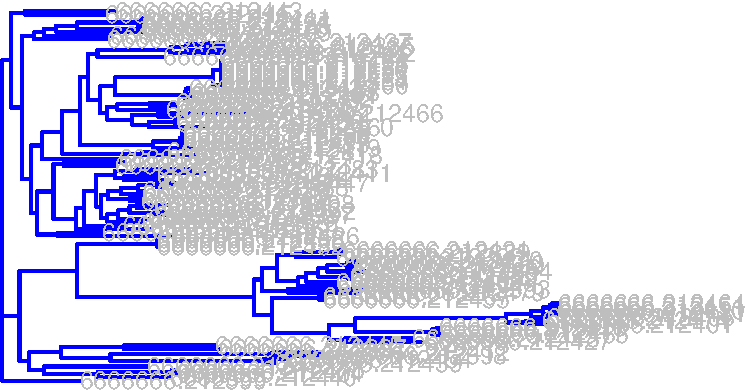
\includegraphics{tesis_files/figure-latex/testingPhylogeny-1} \end{center}
  
  To capture differences on genomes we sort them phylogenetically.
  Phylogenies can be constructed using different paradigms as Parsimony,
  Maximum Likelihood, and Bayesian inference. Short descriptions of the
  main phylogeny methods are included below.
  
  Why is a tree useful \{Book reference\} why trees are useful for?\\
  * Distance methods\\
  * Parsimony * Maximum Likelihood * Mr bayes
  
  General Trees\\
  Actinobacteria Tree, ArchaeaTree, CyanobacteriaTree.
  
  It's easy to create a list. It can be unordered like
  
  To create a sublist, just indent the values a bit (at least four spaces
  or a tab). (Here's one case where indentation is key!)
  
  \begin{enumerate}
  \def\labelenumi{\arabic{enumi}.}
  \tightlist
  \item
    Item 1
  \item
    Item 2
  \item
    Item 3
  
    \begin{itemize}
    \tightlist
    \item
      Item 3a
    \item
      Item 3b
    \end{itemize}
  \end{enumerate}
  
  \subsubsection{Central DB}\label{central-db}
  
  We chose central pathways from
  {[}\protect\hyperlink{ref-barona-gomezux5fwhatux5f2012}{137}{]}\\
  * BBH Best Bidirectional Hits with studied enzymes from Central
  Actinobacterial pathways were selected.
  
  \begin{itemize}
  \item
    By abundance
  \item
    By expansions on genomes
  \end{itemize}
  
  {[}largefiles,\url{https://help.github.com/articles/installing-git-large-file-storage/}{]}
  
  \section{Data Bases}\label{data-bases}
  
  \subsection{Central pathways}\label{central-pathways}
  
  Central database were chosen by BBH from -Actino\\
  Corynebacterium glutamicum\\
  242137 6666666.112876 Streptomyces coelicolor A3(2) NC\_003888.3 1
  8667507 2015-03-27\\
  288055 6666666.146923 Mycobacterium tuberculosis H37Rv NC\_000962.3 1
  4411532
  
  -Archaea closed\\
  390224 6666666.211599 Methanosarcina acetivorans C2A C2A AE010299.1 1
  5751492 SELECTED Euryarchaeota Methanomicrobia\\
  390346 6666666.211718 Nanoarchaeum equitans Kin4-M - AE017199.1 1 490885
  SELECTED DPANN group Nanoarchaeota\\
  390660 6666666.211909 Natronomonas pharaonis DSM 2160 Gabara CR936257.1
  1 2595221 SELECTED Euryarchaeota Halobacteria\\
  390189 6666666.211567 Sulfolobus solfataricus P2 P2 AE006641.1 1 2992245
  SELECTED TACK group Crenarchaeota\\
  -Cyanos\\
  391213 6666666.212444 Cyanothece sp. ATCC 51142 CP000806.1 1 4934271
  Cyanobacteria; Oscillatoriophycideae; Oscillatoriales
  
  391246 6666666.212477 Synechococcus sp. PCC 7002 CP000951.1 1 3008047
  Cyanobacteria; Synechococcales; Synechococcaceae
  
  351204 6666666.189647 Arthrospira platensis C1 1 6089210
  
  \subsection{Genome Dynamics}\label{genome-dynamics}
  
  Among BBH central databases, genomic dynamics was included.\\
  Whats change
  site:\href{http://pubseed.theseed.org/wc.cgi?request=show_otus\&base=/homes/nselem/Data/CS}{WC
  Data}
  
  groups were formed with 100Cyanos, 100Archaea , 118 Actinos Closed,
  43StreptosClosed\\
  Selected organims were
  
  \begin{Shaded}
  \begin{Highlighting}[]
  \NormalTok{table <-}\StringTok{ }\KeywordTok{read.csv}\NormalTok{(}\StringTok{"chapter1/WC_Central/WC_Organisms.txt"}\NormalTok{, }\DataTypeTok{row.names =} \DecValTok{1}\NormalTok{,}\DataTypeTok{sep=}\StringTok{"}\CharTok{\textbackslash{}t}\StringTok{"}\NormalTok{)}
  \CommentTok{#kable(table,  caption = "WC_Organisms \textbackslash{}\textbackslash{}label\{tab:WC_Organisms\}",caption.short = "WC_Organisms ")}
  \end{Highlighting}
  \end{Shaded}
  
  Those families present on at least as much as genomes on the group\\
  Cyanos 100 647\\
  Abundant.Families.100Cyanos\\
  Actinos 118 132\\
  Abundant.Families.43Strepto\\
  Archaea 100 35\\
  Abundant.Families.Actinos\\
  Streptomyces 43 1263\\
  Abundant.Families.Archaeas
  
  Those families expanded on at least two groups\\
  \texttt{cat\ *Abun*\ \textbar{}\ cut\ -f3\textbar{}\ sort\ \textbar{}\ uniq\ -c\ \textbar{}\ sort\ \textgreater{}Abundance.all}\\
  
  Those Families expanded on Archaea and not expanded on Actino\\
  \texttt{comm\ -23\ f3Archaeas\ f3Actinos\ \textgreater{}ArchaeasNoActinos}\\
  Those Families expanded on Actino and not on Archaea\\
  \texttt{comm\ -13\ f3Archaeas\ f3Actinos\ \textgreater{}ActinosNoArchaea}
  
  Those families expanded on Streptomyces but not in ActinoBacteria\\
  \texttt{comm\ -13\ f343Strepto\ f3Actinos\ \textgreater{}ActinosNoStrepto}\\
  Those Families expanded on Actinobacteria and not in Streptomyces\\
  \texttt{comm\ -23\ f343Strepto\ f3Actinos\ \textgreater{}StreptoNoActinos}
  
  Those Families expanded on Cyano and not in Actino\\
  \texttt{comm\ -23\ f3Cyanos\ f3Actinos\ \textgreater{}CyanosNoActinos}
  
  \subsubsection{Natural Products DB}\label{natural-products-db}
  
  Natural products was improved from previous version
  
  \subsection{AntisMASH optional DB}\label{antismash-optional-db}
  
  AntiSMASH is
  {[}\protect\hyperlink{ref-weberux5fantismashux5f2015}{138}{]}\\
  \#\#\# Archaeas Results Archaea is a kingdom of recent discovery were
  not many natural products has been known. On Actinobacteria, evoMining
  has proved its value to find new kinds of natural products. The clue to
  this discovery was that Actinobacteria has genomic expanssions. Now
  Archaea has genomic expansions, even more has central pathways genomic
  expansions. Are this expansions derived from a genomic duplication?\\
  Has Archaea natural products detected by antismash, and if not, where
  are this NP's or may Archaea doesn't have NP's.
  
  applying EvoMining to Archaea
  
  \subsection{Otras estrategias para los clusters Argon context
  Idea}\label{otras-estrategias-para-los-clusters-argon-context-idea}
  
  \section{Argonne}\label{argonne}
  
  ssh
  \href{mailto:nselem@login.mcs.anl.gov}{\nolinkurl{nselem@login.mcs.anl.gov}}\\
  phrase\\
  ssh \href{mailto:nselem@maple}{\nolinkurl{nselem@maple}}\\
  password
  
  cs close strain\\
  wc whats chain
  
  we source (edit bashrc)\\
  link ln (create a link to ross directory)\\
  run out of power:\\
  screen
  
  in Seqs (not mine)\\
  cat\\
  6666666.103569 6666666.112815 6666666.112823 6666666.112833
  6666666.112841 6666666.112849 6666666.112857 \textgreater{}
  /home/nse/Concat\_Full\\
  to find paralogous sets\\
   svr\_representative\_sequences -b -f Id\_Clust -s 0.5 \textless{}
  Concat\_Full \textgreater{} TempFull\&\\
   perl -p -i -e `s/\r//' readable.tree to clean the tree\\
  To find contexts o pegs of paralogous sets
  
  Context midle point 5000 bp (using text tables)\\
  scp 6666666.112839.txt
  \href{mailto:nselem@maple}{\nolinkurl{nselem@maple}}:/homes/nselem/Strepto\_01/.
  
  fig\textbar{}6666666.112839.peg.26
  
  copy families.all file\\
  on the file we have column1 family name column 5 peg id
  
  cluster\_objects \textless{} elements\_to\_cluster \textgreater{}
  ClusteFile
  
  write a file with pegs\\
  1 peg1 adjacent1, adjacent2 \ldots{}.\\
  1 peg2\\
  2\\
  2
  
  write a file similiar but with the family number
  
  1 peg1 fn1, fn2 \ldots{}.\\
  1 peg2\\
  2\\
  2
  
  compare each peg on this file from the same family
  
  Write the conextions file\\
  peg1 peg2\\
  peg1 peg3\\
  peg2 peg3
  
  cluster this file and score the cluster
  
  Define
  
  \begin{verbatim}
  1.  a "function set" is generated by the what's changed directory  
  \end{verbatim}
  
  as a ``family''
  
  \begin{verbatim}
  2.  a "paralog set" is a set of function sets in which paralogous  
  \end{verbatim}
  
  members span the sets
  
  \begin{verbatim}
  3.  a PEG is in a paralog set if it is in one ofthe function sets  
  \end{verbatim}
  
  that make up the
  
  \begin{verbatim}
  4.  a "context" of a PEG is the set of close pegs  
  4.1 First cluster operation would give us: context sets  (CS)  
  
  5.  a "context set" is a set of PEGs with "similar contexts"  
  5.1 second clustering operation would give us:cluster  (Cl)  
  
  6.  a "cluster" is a set of context sets (each context set is a different   
  \end{verbatim}
  
  compute:\\
   Compute the context sets that are made from PEGs that occur in PS.\\
   Compute the contexts of PEGs in PS.
  
  cluster these context using the ``similar contexts'' relation
  
  This gives a set of clusters, and the members of the clusters are
  context sets\\
  That is, a cluster is a set of context sets
  
  \begin{verbatim}
    a. the number of contexts sets i  
  \end{verbatim}
  
  score the clusters\\
   Take a paralog set PS.\\
   Be the context sets: CS\_1, CS\_2,\ldots{}, CS\_k members of the
  paralogous set\\
   k the number of contexts sets on the paralogous set\\
   n\_i the cardinality of CS\_i
  
  \begin{verbatim}
  PS={CS1,CS2,...,CS3}  
  Cl={[CS_1,n_1],[CS_2,n_2],...,[CS_k,n_k]}  
  
  let be M=max(n_i)   i=1,2,..k (Maximum cardinality of Context sets)  
      m=max(n_i)   i=1,2,..k, i!=M (second greatest cardinality of context sets)  
      (We are intersted that a second copy is distributed)  
  
  We are interested on k,M,n to form a scoring function for the cluster set  
  S=f(k,m,M)=c_1*k+c_2*m+c_3*M  
  \end{verbatim}
  
  history
  
  Para hacer un nuevo set de datos
  
  591 cd Data/CS\\
   592 mkdir Directorio\\
   593 vi Directorio/rep.genomes\\
   594 cd Directorio/\\
   600 nohup svr\_CS -d Directorio\&
  
  Contenido de rep.genomes\\
  rast\textbar{}390693 nselem35 q8Vf6ib\\
  rast\textbar{}390675 nselem35 q8Vf6ib\\
  rast\textbar{}388811 nselem35 q8Vf6ib
  
  When you click the \textbf{Knit} button above a document will be
  generated that includes both content as well as the output of any
  embedded \textbf{R} code chunks within the document. You can embed an
  \textbf{R} code chunk like this (\texttt{cars} is a built-in \textbf{R}
  dataset):
  
  \begin{Shaded}
  \begin{Highlighting}[]
  \KeywordTok{summary}\NormalTok{(cars)}
  \end{Highlighting}
  \end{Shaded}
  
  \begin{verbatim}
       speed           dist       
   Min.   : 4.0   Min.   :  2.00  
   1st Qu.:12.0   1st Qu.: 26.00  
   Median :15.0   Median : 36.00  
   Mean   :15.4   Mean   : 42.98  
   3rd Qu.:19.0   3rd Qu.: 56.00  
   Max.   :25.0   Max.   :120.00  
  \end{verbatim}
  
  \subsection{Inline code}\label{inline-code}
  
  If you'd like to put the results of your analysis directly into your
  discussion, add inline code like this:
  
  \begin{quote}
  The \texttt{cos} of \(2 \pi\) is 1.
  \end{quote}
  
  Another example would be the direct calculation of the standard
  deviation:
  
  \begin{quote}
  The standard deviation of \texttt{speed} in \texttt{cars} is 5.2876444.
  \end{quote}
  
  One last neat feature is the use of the \texttt{ifelse} conditional
  statement which can be used to output text depending on the result of an
  \textbf{R} calculation:
  
  \begin{quote}
  The standard deviation is less than 6.
  \end{quote}
  
  Note the use of \texttt{\textgreater{}} here, which signifies a
  quotation environment that will be indented.
  
  As you see with \texttt{\$2\ \textbackslash{}pi\$} above, mathematics
  can be added by surrounding the mathematical text with dollar signs.
  More examples of this are in {[}Mathematics and Science{]} if you
  uncomment the code in {[}Math{]}.
  
  \section{Recomendaciones de Luis}\label{recomendaciones-de-luis}
  
  Para evoMining\\
  Probar distintos métodos de filogenia y después hacer la coloración.\\
  maximum likelihood, Protest phyml\\
  Atracción de ramas largas.\\
  raxml\\
  trim all vs Gblocs (Tony Galvadon)
  
  Comparar dos árboles\\
  Para ver si la evolución de los genes concatenados ha sido simultánea\\
  Robinson and foulds\\
  Joe Felsestein\\
  Phylip
  
  \begin{enumerate}
  \def\labelenumi{\arabic{enumi}.}
  \setcounter{enumi}{1}
  \tightlist
  \item
    dist tree\\
    quarter descomposition\\
    peter gogarten fendou Mao
  \end{enumerate}
  
  Sets de experimentos.\\
  Para el experimento de los streptomyces con ruta centrales el core,
  analizar el problema de dominios múltiples.\\
  Dominios\\
  Nan Song, Dannie durand\\
  Después del blast
  
  Para obtener\\
  Pablo Vinuesa: Get Homologues
  
  Burkhordelias y su toxina (Preguntar a Beto)\\
  Cianobacterias y la ruta de fijación de nitrógeno.
  
  Servidor Viernes a las 12:00
  
  \section{CORASON: Other genome Mining tools
  context-based}\label{corason-other-genome-mining-tools-context-based}
  
  \section{CORe Analysis of Syntenic Orthologs to prioritize Natural
  Product-Biosynthetic Gene
  Cluster}\label{core-analysis-of-syntenic-orthologs-to-prioritize-natural-product-biosynthetic-gene-cluster}
  
  Genome fluidity on Bacteria is source of biosynthetic gene clusters
  (BGCs) abundance, in fact almost all bacterial genome sequenced
  contributes with new genes and gene clusters to the Bacterial Pangenome.
  As a consequence of gene diversity helped by sequence technology
  advances, researchers often have a large set of genomes that wish to
  analize in search of a particular gene cluster variation. Answering BGCs
  analysis needs CORASON allows users to find and visualice variations of
  a given gene cluster sorting them according to the conserved core
  phylogeny.
  
  To find cluster variations, given a query protein sequence that belongs
  to a reference cluster, CORASON will search on a Bacterial genome
  database all gene clusters that contains orthologues of the
  query-protein and at least another sequence from the reference cluster.
  Orthologues on variation clusters are coloured within a gradient
  according to its identity percentage with the reference cluster
  sequences.
  
  The cluster core attempts to identify a set of functions conserved on
  this particular biosynthetic BGC. The core genome on a taxonomical group
  is the set of coding sequences that are shared between all group
  members, this definition may be adapted to the cluster core by using a
  set of gene clusters instead of a set of genomes. A report about gene
  function will be provided whenever a cluster core exists also core
  sequences will be concatenated to construct a phylogenetic tree and sort
  variation clusters accordingly.
  
  Functional annotations are provided by RAST annotation service due to
  that CORASON genomic databases must be RAST files. Any archaeal or
  bacterial genome can be RAST annotated either on the website or by
  command line using myrast server.
  
  Finally, in order to provide an easy to install distribution CORASON was
  packaged on docker containerization platform. Software dependencies such
  as BLAST 2.2.30, muscle3.8.3, GBlocksLinux64\_0.91b, quicktree,
  newick-utils-1.6, and CORASON code were wrapped together on CORASON
  docker container.
  \href{https://github.com/nselem/EvoDivMet/wiki}{Tutorial} and software
  are available at nselem/github.
  
  CORASON inputs are a genomic database, a reference cluster and an enzyme
  inside this cluster, outputs are newick trees, core functional report
  and a cluster variation SVG file. SVG format among being high quality
  scalable graphics, also allow to display metadata such as gene function
  and genome coordinates just by mouse over figures on a browser
  facilitating genomic analysis.
  
  In conclusion CORASON is an easy to install comparative genomic visual
  tool on a customizable genome database that allows users to visualice
  variations of a reference gene cluster identifing its core functions and
  finally sorting variations according to their evolutionary history
  helping to prioritize clusters that may be involved on chemical novelty.
  
  You can also embed plots. For example, here is a way to use the base
  \textbf{R} graphics package to produce a plot using the built-in
  \texttt{pressure} dataset:
  
  \begin{center}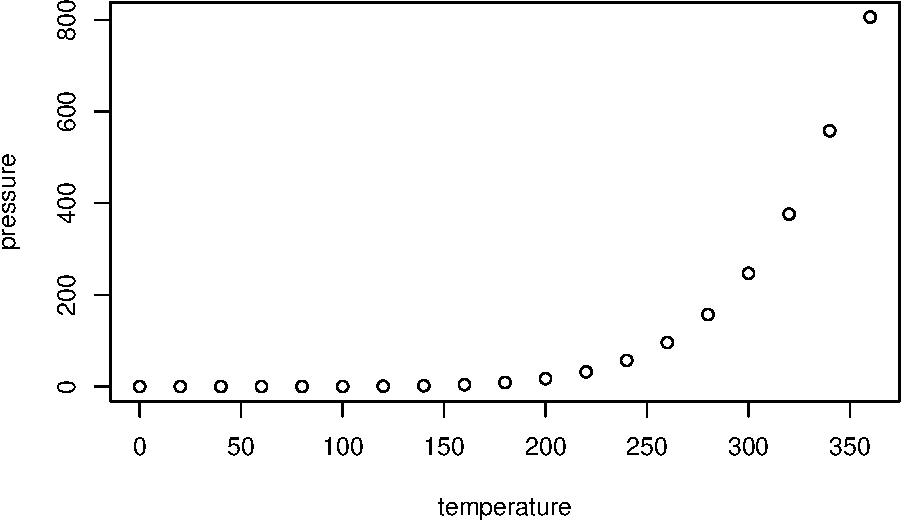
\includegraphics{tesis_files/figure-latex/pressure-1} \end{center}
  
  Note that the \texttt{echo\ =\ FALSE} parameter was added to the code
  chunk to prevent printing of the \textbf{R} code that generated the
  plot. There are plenty of other ways to add chunk options. More
  information is available at \url{http://yihui.name/knitr/options/}.
  
  Another useful chunk option is the setting of \texttt{cache\ =\ TRUE} as
  you see here. If document rendering becomes time consuming due to long
  computations or plots that are expensive to generate you can use knitr
  caching to improve performance. Later in this file, you'll see a way to
  reference plots created in \textbf{R} or external figures.
  
  \section{Loading and exploring data}\label{loading-and-exploring-data}
  
  Included in this template is a file called \texttt{flights.csv}. This
  file includes a subset of the larger dataset of information about all
  flights that departed from Seattle and Portland in 2014. More
  information about this dataset and its \textbf{R} package is available
  at \url{http://github.com/ismayc/pnwflights14}. This subset includes
  only Portland flights and only rows that were complete with no missing
  values. Merges were also done with the \texttt{airports} and
  \texttt{airlines} data sets in the \texttt{pnwflights14} package to get
  more descriptive airport and airline names.
  
  We can load in this data set using the following command:
  
  \begin{Shaded}
  \begin{Highlighting}[]
  \NormalTok{flights <-}\StringTok{ }\KeywordTok{read.csv}\NormalTok{(}\StringTok{"data/flights.csv"}\NormalTok{)}
  \end{Highlighting}
  \end{Shaded}
  
  The data is now stored in the data frame called \texttt{flights} in
  \textbf{R}. To get a better feel for the variables included in this
  dataset we can use a variety of functions. Here we can see the
  dimensions (rows by columns) and also the names of the columns.
  
  \begin{Shaded}
  \begin{Highlighting}[]
  \KeywordTok{dim}\NormalTok{(flights)}
  \end{Highlighting}
  \end{Shaded}
  
  \begin{verbatim}
  [1] 52808    16
  \end{verbatim}
  
  \begin{Shaded}
  \begin{Highlighting}[]
  \KeywordTok{names}\NormalTok{(flights)}
  \end{Highlighting}
  \end{Shaded}
  
  \begin{verbatim}
   [1] "month"        "day"          "dep_time"     "dep_delay"   
   [5] "arr_time"     "arr_delay"    "carrier"      "tailnum"     
   [9] "flight"       "dest"         "air_time"     "distance"    
  [13] "hour"         "minute"       "carrier_name" "dest_name"   
  \end{verbatim}
  
  Another good idea is to take a look at the dataset in table form. With
  this dataset having more than 50,000 rows, we won't explicitly show the
  results of the command here. I recommend you enter the command into the
  Console \textbf{\emph{after}} you have run the \textbf{R} chunks above
  to load the data into \textbf{R}.
  
  \begin{Shaded}
  \begin{Highlighting}[]
  \KeywordTok{View}\NormalTok{(flights)}
  \end{Highlighting}
  \end{Shaded}
  
  While not required, it is highly recommended you use the \texttt{dplyr}
  package to manipulate and summarize your data set as needed. It uses a
  syntax that is easy to understand using chaining operations. Below I've
  created a few examples of using \texttt{dplyr} to get information about
  the Portland flights in 2014. You will also see the use of the
  \texttt{ggplot2} package, which produces beautiful, high-quality
  academic visuals.
  
  We begin by checking to ensure that needed packages are installed and
  then we load them into our current working environment:
  
  \begin{Shaded}
  \begin{Highlighting}[]
  \CommentTok{# List of packages required for this analysis}
  \NormalTok{pkg <-}\StringTok{ }\KeywordTok{c}\NormalTok{(}\StringTok{"dplyr"}\NormalTok{, }\StringTok{"ggplot2"}\NormalTok{, }\StringTok{"knitr"}\NormalTok{, }\StringTok{"devtools"}\NormalTok{)}
  \CommentTok{# Check if packages are not installed and assign the}
  \CommentTok{# names of the packages not installed to the variable new.pkg}
  \NormalTok{new.pkg <-}\StringTok{ }\NormalTok{pkg[!(pkg %in%}\StringTok{ }\KeywordTok{installed.packages}\NormalTok{())]}
  \CommentTok{# If there are any packages in the list that aren't installed,}
  \CommentTok{# install them}
  \NormalTok{if (}\KeywordTok{length}\NormalTok{(new.pkg))}
    \KeywordTok{install.packages}\NormalTok{(new.pkg, }\DataTypeTok{repos =} \StringTok{"http://cran.rstudio.com"}\NormalTok{)}
  \CommentTok{# Load packages}
  \KeywordTok{library}\NormalTok{(dplyr)}
  \KeywordTok{library}\NormalTok{(ggplot2)}
  \KeywordTok{library}\NormalTok{(knitr)}
  \end{Highlighting}
  \end{Shaded}
  
  The example we show here does the following:
  
  \begin{itemize}
  \item
    Selects only the \texttt{carrier\_name} and \texttt{arr\_delay} from
    the \texttt{flights} dataset and then assigns this subset to a new
    variable called \texttt{flights2}.
  \item
    Using \texttt{flights2}, we determine the largest arrival delay for
    each of the carriers.
  \end{itemize}
  
  \begin{Shaded}
  \begin{Highlighting}[]
  \NormalTok{flights2 <-}\StringTok{ }\NormalTok{flights %>%}\StringTok{ }\NormalTok{dplyr::}\KeywordTok{select}\NormalTok{(carrier_name, arr_delay)}
  \NormalTok{max_delays <-}\StringTok{ }\NormalTok{flights2 %>%}\StringTok{ }\KeywordTok{group_by}\NormalTok{(carrier_name) %>%}
  \StringTok{  }\KeywordTok{summarize}\NormalTok{(}\DataTypeTok{max_arr_delay =} \KeywordTok{max}\NormalTok{(arr_delay, }\DataTypeTok{na.rm =} \OtherTok{TRUE}\NormalTok{))}
  \end{Highlighting}
  \end{Shaded}
  
  We next introduce a useful function in the \texttt{knitr} package for
  making nice tables in \emph{R Markdown} called \texttt{kable}. It
  produces the \LaTeX~code required to make the table and is much easier
  to use than manually entering values into a table by copying and pasting
  values into Excel or \LaTeX. This again goes to show how nice
  reproducible documents can be! There is no need to copy-and-paste values
  to create a table. (Note the use of \texttt{results\ =\ "asis"} here
  which will produce the table instead of the code to create the table.
  You'll learn more about the
  \texttt{\textbackslash{}\textbackslash{}label} later.) The
  \texttt{caption.short} argument is used to include a shorter version of
  the title to appear in the List of Tables at the beginning of the
  document.
  
  \begin{Shaded}
  \begin{Highlighting}[]
  \KeywordTok{kable}\NormalTok{(max_delays, }\DataTypeTok{col.names =} \KeywordTok{c}\NormalTok{(}\StringTok{"Airline"}\NormalTok{, }\StringTok{"Max Arrival Delay"}\NormalTok{),}
        \DataTypeTok{caption =} \StringTok{"Maximum Delays by Airline }\CharTok{\textbackslash{}\textbackslash{}}\StringTok{label\{tab:max_delay\}"}\NormalTok{,}
        \DataTypeTok{caption.short =} \StringTok{"Max Delays by Airline"}\NormalTok{)}
  \end{Highlighting}
  \end{Shaded}
  
  \begin{longtable}[c]{@{}lr@{}}
  \caption{Maximum Delays by Airline \label{tab:max_delay}}\tabularnewline
  \toprule
  Airline & Max Arrival Delay\tabularnewline
  \midrule
  \endfirsthead
  \toprule
  Airline & Max Arrival Delay\tabularnewline
  \midrule
  \endhead
  Alaska Airlines Inc. & 338\tabularnewline
  American Airlines Inc. & 1539\tabularnewline
  Delta Air Lines Inc. & 651\tabularnewline
  Frontier Airlines Inc. & 575\tabularnewline
  Hawaiian Airlines Inc. & 407\tabularnewline
  JetBlue Airways & 273\tabularnewline
  SkyWest Airlines Inc. & 421\tabularnewline
  Southwest Airlines Co. & 694\tabularnewline
  United Air Lines Inc. & 472\tabularnewline
  US Airways Inc. & 347\tabularnewline
  Virgin America & 366\tabularnewline
  \bottomrule
  \end{longtable}
  
  We can further look into the properties of the largest value here for
  American Airlines Inc. To do so, we can isolate the row corresponding to
  the arrival delay of 1539 minutes for American in our original
  \texttt{flights} dataset.
  
  \begin{Shaded}
  \begin{Highlighting}[]
  \NormalTok{flights %>%}\StringTok{ }\NormalTok{dplyr::}\KeywordTok{filter}\NormalTok{(arr_delay ==}\StringTok{ }\DecValTok{1539}\NormalTok{, }
                     \NormalTok{carrier_name ==}\StringTok{ "American Airlines Inc."}\NormalTok{) %>%}
  \StringTok{  }\NormalTok{dplyr::}\KeywordTok{select}\NormalTok{(-}\KeywordTok{c}\NormalTok{(month, day, carrier, dest_name, hour, }
              \NormalTok{minute, carrier_name, arr_delay))}
  \end{Highlighting}
  \end{Shaded}
  
  \begin{verbatim}
    dep_time dep_delay arr_time tailnum flight dest air_time distance
  1     1403      1553     1934  N595AA   1568  DFW      182     1616
  \end{verbatim}
  
  We see that the flight occurred on March 3rd and departed a little after
  2 PM on its way to Dallas/Fort Worth. Lastly, we show how we can
  visualize the arrival delay of all departing flights from Portland on
  March 3rd against time of departure.
  
  \begin{Shaded}
  \begin{Highlighting}[]
  \NormalTok{flights %>%}\StringTok{ }\NormalTok{dplyr::}\KeywordTok{filter}\NormalTok{(month ==}\StringTok{ }\DecValTok{3}\NormalTok{, day ==}\StringTok{ }\DecValTok{3}\NormalTok{) %>%}
  \StringTok{  }\KeywordTok{ggplot}\NormalTok{(}\KeywordTok{aes}\NormalTok{(}\DataTypeTok{x =} \NormalTok{dep_time, }\DataTypeTok{y =} \NormalTok{arr_delay)) +}
  \StringTok{  }\KeywordTok{geom_point}\NormalTok{()}
  \end{Highlighting}
  \end{Shaded}
  
  \begin{center}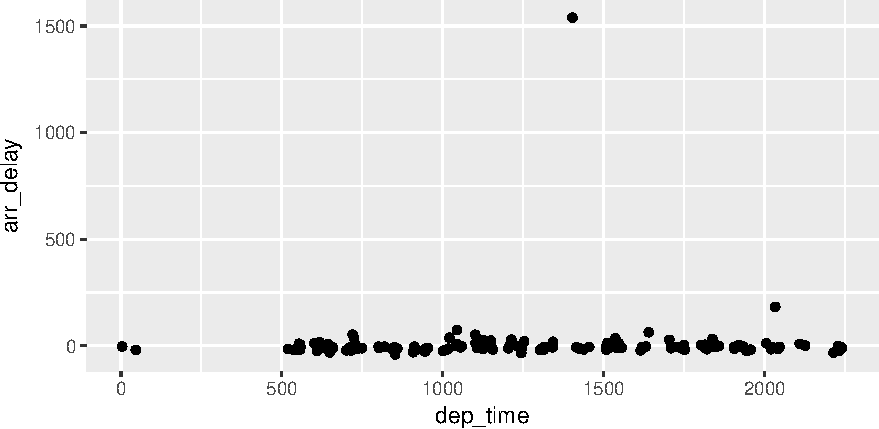
\includegraphics{tesis_files/figure-latex/march3plot-1} \end{center}
  
  \chapter{PriA Family}\label{math-sci}
  
  PriA isomerase is a promiscuous enzyme involved in histidine and
  Triptophan pathways. This enzyme family catalize convertions HisA and
  TrpF converting ProFAR on and PRA into products. PriA can be found at
  Actinobacteria phylum.
  
  \begin{Shaded}
  \begin{Highlighting}[]
  \CommentTok{# List of packages required for this analysis}
  \NormalTok{pkg <-}\StringTok{ }\KeywordTok{c}\NormalTok{(}\StringTok{"dplyr"}\NormalTok{, }\StringTok{"ggplot2"}\NormalTok{, }\StringTok{"knitr"}\NormalTok{, }\StringTok{"devtools"}\NormalTok{,}\StringTok{"RColorBrewer"}\NormalTok{)}
  \CommentTok{# Check if packages are not installed and assign the}
  \CommentTok{# names of the packages not installed to the variable new.pkg}
  \NormalTok{new.pkg <-}\StringTok{ }\NormalTok{pkg[!(pkg %in%}\StringTok{ }\KeywordTok{installed.packages}\NormalTok{())]}
  \CommentTok{# If there are any packages in the list that aren't installed,}
  \CommentTok{# install them}
  \NormalTok{if (}\KeywordTok{length}\NormalTok{(new.pkg))}
    \KeywordTok{install.packages}\NormalTok{(new.pkg, }\DataTypeTok{repos =} \StringTok{"http://cran.rstudio.com"}\NormalTok{)}
  \CommentTok{# Load packages}
  \KeywordTok{library}\NormalTok{(dplyr)}
  \KeywordTok{library}\NormalTok{(plyr)}
  \KeywordTok{library}\NormalTok{(reshape)}
  \KeywordTok{library}\NormalTok{(ggplot2)}
  \KeywordTok{library}\NormalTok{(knitr)}
  \KeywordTok{library}\NormalTok{(RColorBrewer)}
  \NormalTok{hm.palette <-}\StringTok{ }\KeywordTok{colorRampPalette}\NormalTok{(}\KeywordTok{rev}\NormalTok{(}\KeywordTok{brewer.pal}\NormalTok{(}\DecValTok{11}\NormalTok{, }\StringTok{'Spectral'}\NormalTok{)), }\DataTypeTok{space=}\StringTok{'Lab'}\NormalTok{)  }
  \KeywordTok{library}\NormalTok{(genstats) ## Next libraries are for coursera}
  \KeywordTok{library}\NormalTok{(devtools)}
  \KeywordTok{library}\NormalTok{(Biobase)}
  \KeywordTok{library}\NormalTok{(scales) }\CommentTok{# }
  \KeywordTok{library}\NormalTok{(xlsx) }\CommentTok{# For save data on excel}
  \end{Highlighting}
  \end{Shaded}
  
  \section{Methods}\label{methods}
  
  52 Streptomyces genera has differences on PriA funcion. PriA \#\# Math
  Docking simulation were calculated for Streptomyces enzymes. TrpF
  enzymes from Strptomyces Mg1, Jonesia denitrificans, were added as
  controls
  
  Procedures can be found at
  \href{https://github.com/tripplab/Docking/wiki}{Docking Protocols}
  
  1.Phylogenetic Tree 39 Streptomyces sequences, as outgroup E coli,
  Arthrobacter Aurescens, Salmonella enterica and Acidimicrobium
  ferrooxidans PriA's were included.
  
  CORASON PriA All streptomyces have a partially conserved PriA cluster.
  CT34 has a secondary copy whose Best hit on NCBI is Lentzea's PriA with
  50\% identity 98\% coverage
  
  TrpF1 TrpF1 queries gave hits with TrpC enzyme present on every
  Streptomyces, additionally S rimosus, S coelicolor, S venezuelae and S.
  NRRL S-1813 had an extra copy. S rimosus TrpC vicinity has PKS and
  siderophore genes.
  
  TrpF2 Conserved cluster with NRPS sequences flanking TrpF2
  
  TrpF3 Non conserved cluster
  
  TrpF4 purpeofuscus and S bikiniensis 2. Heatmap
  
  Additionally to the sequences selected by phylogeny, Jonesia
  denitrificans and Streptomyces sp Mg1 TrpF sequences were added as
  control .
  
  Substrate table
  
  \begin{Shaded}
  \begin{Highlighting}[]
  \NormalTok{table <-}\StringTok{ }\KeywordTok{read.csv}\NormalTok{(}\StringTok{"chapter2/Substrate.data"}\NormalTok{, }\DataTypeTok{row.names =} \DecValTok{1}\NormalTok{,}\DataTypeTok{sep=}\StringTok{"}\CharTok{\textbackslash{}t}\StringTok{"}\NormalTok{)}
  \KeywordTok{kable}\NormalTok{(table,  }\DataTypeTok{caption =} \StringTok{"Substrates }\CharTok{\textbackslash{}\textbackslash{}}\StringTok{label\{tab:substrates\}"}\NormalTok{,}\DataTypeTok{caption.short =} \StringTok{"Substrates "}\NormalTok{)}
  \end{Highlighting}
  \end{Shaded}
  
  \begin{longtable}[c]{@{}lllllll@{}}
  \caption{Substrates \label{tab:substrates}}\tabularnewline
  \toprule
  & id & Number & Kind & Reference & Names & Observations\tabularnewline
  \midrule
  \endfirsthead
  \toprule
  & id & Number & Kind & Reference & Names & Observations\tabularnewline
  \midrule
  \endhead
  S13 & dte6\_open & LUZ & & & & NA\tabularnewline
  S15 & dte13\_open & LUZ & & & & NA\tabularnewline
  S14 & dte6\_closed & LUZ & & & & NA\tabularnewline
  S16 & dte13\_closed & LUZ & & & & NA\tabularnewline
  S10 & C04376 & & James & & 5'-Phosphoribosyl-N-formylglycinamide &
  NA\tabularnewline
  S12 & C03838 & & James & & 5'-Phosphoribosylglycinamide &
  NA\tabularnewline
  S9 & C04640 & & James & &
  2-(Formamido)-N1-(5'-phosphoribosyl)acetamidine & NA\tabularnewline
  S18 & CompoundV & & Adams & CompundV & This compound is an intermediary
  between GTP and H2NMP & NA\tabularnewline
  S5 & C05923 & & James & & 2,5-Diaminopyrimidine nucleoside triphosphate
  & NA\tabularnewline
  S4 & C05922 & & James & & Formamidopyrimidine nucleoside triphosphate &
  NA\tabularnewline
  S8 & C01268 & & James & & 5-Amino-6-(5'-phosphoribosylamino)uracil &
  NA\tabularnewline
  S17 & PraP & & Verduzco & PraP & & NA\tabularnewline
  S7 & C04302 & & James & & PRA & NA\tabularnewline
  S6 & C00144 & & James & & GMP & NA\tabularnewline
  S11 & C00044 & & James & & GTP & NA\tabularnewline
  S1 & C01253 & & James & & ADP-D-ribosyl-{[}dinitrogen reductase{]} &
  NA\tabularnewline
  S2 & C01201 & & James & & N(omega)-(ADP-D-ribosyl)-L-arginine &
  NA\tabularnewline
  S3 & C04896 & & & & ProFAR & NA\tabularnewline
  S19 & S\_17146 & & Due et al & 17146 &
  2,5-dimethyl-N-(4-oxocyclohexa-2,5-dienylidene)benzenesulfonamide
  \#17146, 4456-2380, Chem-Div & NA\tabularnewline
  S20 & S\_16827 & & Due et al & 16827 &
  (E)-N-(3-chloro-5-methyl-4-oxocyclohexa-2,5-dienylidene)
  benzenesulfonamide, \#16827, 3993-4586, Chem-Div & NA\tabularnewline
  mrBaye & s PriAjulian.nx & s on mazo & rca goes to & PriAjulian.c &
  on.tre &\tabularnewline
  PriAju & lian.con.tre wa & s open wi & th figtree a & nd saved as & SVG
  &\tabularnewline
  To get & coordinates: ` & coordtree & .pl PriAjuli & an.SVG` &
  &\tabularnewline
  Heatpl & ot color are fr & om ggplot & R & & &\tabularnewline
  mydata & .xls lo guardoe & n mydata. & cvs & & &\tabularnewline
  perl r & ead\_mydata.pl m & ydata.cvs & \textgreater{}Heat.color & s &
  &\tabularnewline
  mnuall & y edit Heat.col & ors by ad & ding headers & enzymas y s &
  ubstrates &\tabularnewline
  perl h & eatFromRGB.pl H & eatColor & YPriAJulian & & &\tabularnewline
  Hice e & l heatplot en S & VG con el & script & & &\tabularnewline
  \bottomrule
  \end{longtable}
  
  Observaciones Mauricio\\
  - falta el pie de figura Substrate docking over enzymes from extended
  PriA families. Substrates 1-20
  
  \begin{itemize}
  \item
    falta el dendograma arriba de los sustratos (indicar cuál es pra y
    cuál profar)
  \item
    falta la escala de colores (con valores y unidades). Cuando agregues
    el dendograma de los sutratos va a quedar un cuadrante vacío en la
    parte superior izquierda, en ese espacio pon la escala de forma
    horizontal
  \item
    intenta aumentar el contraste de color entre el valor mínimo y máximo
    de la escala\\
    Intente varias Figuras
  \item
    repite las etiquetas de los sutratos abajo del heatmap\\
    Pendiende
  \item
    hay inconsistencias en los nombres de la enzimas (eg, Ssvi y Svi, SMgl
    y Smgl, etc)\\
    Árbol nuevo sin datos faltantes
  \item
    para el caso de las enzimas sin datos, usa negro en lugar de
    amarillo\\
    LISTO
  \item
    ``Controles TrpF/subTrpF'' (debe estar en inglés), puede ser confuso
    poner dos etiquetas para la misma función
  \end{itemize}
  
  \begin{Shaded}
  \begin{Highlighting}[]
  \NormalTok{docking <-}\StringTok{ }\KeywordTok{read.csv}\NormalTok{(}\StringTok{"chapter2/SmallHeat.data"}\NormalTok{, }\DataTypeTok{header=}\OtherTok{TRUE}\NormalTok{, }\DataTypeTok{sep=}\StringTok{"}\CharTok{\textbackslash{}t}\StringTok{"}\NormalTok{)}
  \NormalTok{EnzymeOrder=}\KeywordTok{factor}\NormalTok{(docking$Enzima,}\DataTypeTok{levels=}\KeywordTok{unique}\NormalTok{(docking$Enzima))}
  \NormalTok{docking.m <-}\StringTok{ }\KeywordTok{melt}\NormalTok{(docking,}\DataTypeTok{id =} \StringTok{"Enzima"}\NormalTok{)}
  \NormalTok{docking.m <-}\StringTok{ }\KeywordTok{ddply}\NormalTok{(docking.m, .(variable), transform,}\DataTypeTok{rescale =} \KeywordTok{rescale}\NormalTok{(value))}
  \NormalTok{docking.m$Enzima <-}\StringTok{ }\KeywordTok{factor}\NormalTok{(docking.m$Enzima, }\DataTypeTok{levels =} \KeywordTok{rev}\NormalTok{(docking.m$Enzima[}\KeywordTok{order}\NormalTok{(EnzymeOrder)]))}
  
  \NormalTok{################# on white and blue}
  \NormalTok{blueHeatPlot<-}\KeywordTok{ggplot}\NormalTok{(docking.m, }\KeywordTok{aes}\NormalTok{(}\DataTypeTok{x=}\NormalTok{variable, }\DataTypeTok{y=}\NormalTok{Enzima)) +}\StringTok{ }\KeywordTok{labs}\NormalTok{(}\DataTypeTok{x =} \StringTok{"Substrates"}\NormalTok{, }\DataTypeTok{y =} \StringTok{"Enzymes"}\NormalTok{,}\DataTypeTok{text =} \KeywordTok{element_text}\NormalTok{(}\DataTypeTok{size=}\DecValTok{12}\NormalTok{))+}\StringTok{ }\KeywordTok{geom_raster}\NormalTok{(}\KeywordTok{aes}\NormalTok{(}\DataTypeTok{fill=}\NormalTok{value))+}\KeywordTok{scale_fill_gradient}\NormalTok{(}\DataTypeTok{low =} \StringTok{"white"}\NormalTok{, }\DataTypeTok{high =} \StringTok{"steelblue"}\NormalTok{,}\DataTypeTok{na.value =} \StringTok{"black"}\NormalTok{)+}\KeywordTok{theme_bw}\NormalTok{()+}\KeywordTok{theme}\NormalTok{(}\DataTypeTok{plot.title =} \KeywordTok{element_text}\NormalTok{(}\DataTypeTok{size =} \DecValTok{14}\NormalTok{, }\DataTypeTok{face =} \StringTok{"bold"}\NormalTok{), }\DataTypeTok{text =} \KeywordTok{element_text}\NormalTok{(}\DataTypeTok{size =} \DecValTok{12}\NormalTok{), }\DataTypeTok{axis.title =} \KeywordTok{element_text}\NormalTok{(}\DataTypeTok{face=}\StringTok{"bold"}\NormalTok{), }\DataTypeTok{axis.text.x=}\KeywordTok{element_text}\NormalTok{(}\DataTypeTok{angle =} \DecValTok{90}\NormalTok{,}\DataTypeTok{size =} \DecValTok{6}\NormalTok{))}
  \KeywordTok{ggsave}\NormalTok{(}\StringTok{"chapter2/blueHeatPlot.pdf"}\NormalTok{, }\DataTypeTok{plot =} \NormalTok{blueHeatPlot,}\DataTypeTok{height =} \DecValTok{36}\NormalTok{, }\DataTypeTok{width =} \DecValTok{24}\NormalTok{)}
  
  
   \NormalTok{## black and white}
  \NormalTok{blackHeatPlot<-}\KeywordTok{ggplot}\NormalTok{(docking.m, }\KeywordTok{aes}\NormalTok{(}\DataTypeTok{x=}\NormalTok{variable, }\DataTypeTok{y=}\NormalTok{Enzima)) +}\StringTok{ }\KeywordTok{labs}\NormalTok{(}\DataTypeTok{x =} \StringTok{"Substrates"}\NormalTok{, }\DataTypeTok{y =} \StringTok{"Enzymes"}\NormalTok{,}\DataTypeTok{text =} \KeywordTok{element_text}\NormalTok{(}\DataTypeTok{size=}\DecValTok{12}\NormalTok{))+}\StringTok{ }\KeywordTok{geom_raster}\NormalTok{(}\KeywordTok{aes}\NormalTok{(}\DataTypeTok{fill=}\NormalTok{value))+}\KeywordTok{scale_fill_gradient}\NormalTok{(}\DataTypeTok{low =} \StringTok{"white"}\NormalTok{, }\DataTypeTok{high =} \StringTok{"black"}\NormalTok{,}\DataTypeTok{na.value =} \StringTok{"black"}\NormalTok{)+}\KeywordTok{theme_bw}\NormalTok{()+}\KeywordTok{theme}\NormalTok{(}\DataTypeTok{plot.title =} \KeywordTok{element_text}\NormalTok{(}\DataTypeTok{size =} \DecValTok{14}\NormalTok{, }\DataTypeTok{face =} \StringTok{"bold"}\NormalTok{), }\DataTypeTok{text =} \KeywordTok{element_text}\NormalTok{(}\DataTypeTok{size =} \DecValTok{12}\NormalTok{), }\DataTypeTok{axis.title =} \KeywordTok{element_text}\NormalTok{(}\DataTypeTok{face=}\StringTok{"bold"}\NormalTok{), }\DataTypeTok{axis.text.x=}\KeywordTok{element_text}\NormalTok{(}\DataTypeTok{angle =} \DecValTok{90}\NormalTok{,}\DataTypeTok{size =} \DecValTok{6}\NormalTok{))}
  \KeywordTok{ggsave}\NormalTok{(}\StringTok{"chapter2/blackHeatPlot.pdf"}\NormalTok{, }\DataTypeTok{plot =} \NormalTok{blackHeatPlot,}\DataTypeTok{height =} \DecValTok{36}\NormalTok{, }\DataTypeTok{width =} \DecValTok{24}\NormalTok{)}
  
  \NormalTok{g <-}\StringTok{ }\KeywordTok{ggplot_build}\NormalTok{(blackHeatPlot)}
  \NormalTok{g$data[[}\DecValTok{1}\NormalTok{]][}\StringTok{"fill"}\NormalTok{]}
  \end{Highlighting}
  \end{Shaded}
  
  \begin{verbatim}
          fill
  1    #636363
  2    #636363
  3    #676767
  4    #7C7C7C
  5      black
  6    #595959
  7    #A6A6A6
  8    #484848
  9    #5C5C5C
  10   #B6B6B6
  11   #484848
  12     black
  13     black
  14   #313131
  15   #3E3E3E
  16   #636363
  17   #525252
  18   #848484
  19   #606060
  20   #9A9A9A
  21   #373737
  22   #9E9E9E
  23   #484848
  24   #717171
  25   #636363
  26   #6A6A6A
  27   #676767
  28   #3E3E3E
  29   #606060
  30   #797979
  31   #676767
  32   #797979
  33   #717171
  34   #636363
  35   #676767
  36   #414141
  37   #444444
  38     black
  39   #3A3A3A
  40   #414141
  41   #6A6A6A
  42   #4E4E4E
  43   #525252
  44   #C6C6C6
  45   #939393
  46   #808080
  47   #C6C6C6
  48   #636363
  49   #A6A6A6
  50   #676767
  51     black
  52   #808080
  53   #DEDEDE
  54   #C2C2C2
  55   #2B2B2B
  56   #A2A2A2
  57   #BABABA
  58   #848484
  59   #808080
  60   #5C5C5C
  61   #8B8B8B
  62   #606060
  63   #5C5C5C
  64   #676767
  65   #636363
  66     black
  67   #6A6A6A
  68   #939393
  69   #606060
  70   #4B4B4B
  71   #EAEAEA
  72   #484848
  73     black
  74     black
  75   #808080
  76   #595959
  77   #4B4B4B
  78   #676767
  79   #6A6A6A
  80   #979797
  81   #484848
  82   #4E4E4E
  83   #525252
  84   #808080
  85   #5C5C5C
  86   #4E4E4E
  87   #595959
  88   #4B4B4B
  89   #4E4E4E
  90   #555555
  91   #606060
  92   #555555
  93   #595959
  94   #5C5C5C
  95   #525252
  96   #525252
  97   #555555
  98   #525252
  99     black
  100  #4E4E4E
  101  #6E6E6E
  102  #4B4B4B
  103  #606060
  104  #4E4E4E
  105  #717171
  106  #8F8F8F
  107  #757575
  108  #DADADA
  109  #797979
  110  #717171
  111  #525252
  112    black
  113  #8B8B8B
  114  #AAAAAA
  115  #A2A2A2
  116  #2E2E2E
  117  #222222
  118  #BABABA
  119  #979797
  120  #797979
  121  #979797
  122  #8F8F8F
  123  #676767
  124  #555555
  125  #757575
  126  #6A6A6A
  127    black
  128  #5C5C5C
  129  #4B4B4B
  130  #555555
  131  #4E4E4E
  132  #9A9A9A
  133  #606060
  134    black
  135    black
  136  #595959
  137  #636363
  138  #636363
  139  #757575
  140  #676767
  141  #676767
  142  #4B4B4B
  143  #525252
  144  #595959
  145  #595959
  146  #6A6A6A
  147  #595959
  148  #676767
  149  #4E4E4E
  150  #555555
  151  #4E4E4E
  152  #525252
  153  #525252
  154  #4B4B4B
  155  #6A6A6A
  156  #606060
  157  #4E4E4E
  158  #595959
  159  #5C5C5C
  160    black
  161  #636363
  162  #636363
  163  #595959
  164  #525252
  165  #676767
  166  #9A9A9A
  167  #B6B6B6
  168  #A6A6A6
  169  #FFFFFF
  170  #6A6A6A
  171  #EAEAEA
  172  #5C5C5C
  173    black
  174  #7C7C7C
  175  #AAAAAA
  176  #BEBEBE
  177  #343434
  178  #414141
  179  #A6A6A6
  180  #808080
  181  #636363
  182  #808080
  183  #979797
  184  #595959
  185  #444444
  186  #555555
  187  #525252
  188    black
  189  #606060
  190  #4B4B4B
  191  #595959
  192  #444444
  193  #595959
  194  #525252
  195    black
  196    black
  197  #484848
  198  #4E4E4E
  199  #606060
  200  #717171
  201  #4E4E4E
  202  #4B4B4B
  203  #4E4E4E
  204  #444444
  205  #4E4E4E
  206  #414141
  207  #606060
  208  #5C5C5C
  209  #636363
  210  #484848
  211  #3E3E3E
  212  #484848
  213  #484848
  214  #484848
  215  #525252
  216  #5C5C5C
  217  #4E4E4E
  218  #4E4E4E
  219  #4B4B4B
  220  #595959
  221    black
  222  #444444
  223  #5C5C5C
  224  #5C5C5C
  225  #4B4B4B
  226  #595959
  227  #222222
  228  #AEAEAE
  229  #636363
  230  #414141
  231  #414141
  232  #5C5C5C
  233  #444444
  234    black
  235  #757575
  236  #5C5C5C
  237  #7C7C7C
  238  #2B2B2B
  239  #1C1C1C
  240  #373737
  241  #4E4E4E
  242  #5C5C5C
  243  #606060
  244  #606060
  245  #444444
  246  #606060
  247  #555555
  248  #4B4B4B
  249    black
  250  #5C5C5C
  251  #636363
  252  #595959
  253  #3A3A3A
  254  #343434
  255  #444444
  256    black
  257    black
  258  #4E4E4E
  259  #6E6E6E
  260  #6E6E6E
  261  #676767
  262  #414141
  263  #555555
  264  #5C5C5C
  265  #4B4B4B
  266  #3E3E3E
  267  #595959
  268  #3A3A3A
  269  #5C5C5C
  270  #3A3A3A
  271  #4E4E4E
  272  #525252
  273  #444444
  274  #5C5C5C
  275  #484848
  276  #484848
  277  #636363
  278  #606060
  279  #444444
  280  #6E6E6E
  281  #444444
  282    black
  283  #717171
  284  #6A6A6A
  285  #595959
  286  #797979
  287  #717171
  288  #8F8F8F
  289  #414141
  290  #6A6A6A
  291  #808080
  292  #1C1C1C
  293  #676767
  294  #888888
  295    black
  296  #2B2B2B
  297  #5C5C5C
  298  #636363
  299  #4B4B4B
  300  #797979
  301  #5C5C5C
  302  #3A3A3A
  303  #373737
  304  #3A3A3A
  305  #595959
  306  #3A3A3A
  307  #414141
  308  #3A3A3A
  309  #4E4E4E
  310    black
  311  #4E4E4E
  312  #6E6E6E
  313  #595959
  314  #484848
  315  #3A3A3A
  316  #3E3E3E
  317    black
  318    black
  319  #555555
  320  #525252
  321  #444444
  322  #606060
  323  #555555
  324  #444444
  325  #5C5C5C
  326  #3E3E3E
  327  #5C5C5C
  328  #636363
  329  #444444
  330  #636363
  331  #444444
  332  #555555
  333  #525252
  334  #606060
  335  #4B4B4B
  336  #4B4B4B
  337  #4E4E4E
  338  #525252
  339  #484848
  340  #484848
  341  #3E3E3E
  342  #525252
  343    black
  344  #4E4E4E
  345  #676767
  346  #444444
  347  #757575
  348  #606060
  349  #606060
  350  #313131
  351  #676767
  352  #5C5C5C
  353  #222222
  354  #6A6A6A
  355  #797979
  356    black
  357  #252525
  358  #4E4E4E
  359  #595959
  360  #3A3A3A
  361  #606060
  362  #484848
  363  #373737
  364  #252525
  365  #2B2B2B
  366  #595959
  367  #444444
  368  #555555
  369  #444444
  370  #595959
  371    black
  372  #525252
  373  #5C5C5C
  374  #4E4E4E
  375  #313131
  376  #4B4B4B
  377  #444444
  378    black
  379    black
  380  #6A6A6A
  381  #484848
  382  #4E4E4E
  383  #6E6E6E
  384  #3A3A3A
  385  #444444
  386  #3A3A3A
  387  #4B4B4B
  388  #484848
  389  #595959
  390  #525252
  391  #717171
  392  #525252
  393  #4B4B4B
  394  #484848
  395  #484848
  396  #373737
  397  #525252
  398  #4B4B4B
  399  #636363
  400  #676767
  401  #444444
  402  #3A3A3A
  403  #414141
  404    black
  405  #4B4B4B
  406  #5C5C5C
  407  #484848
  408  #6E6E6E
  409  #5C5C5C
  410  #717171
  411  #282828
  412  #6A6A6A
  413  #555555
  414  #1C1C1C
  415  #6E6E6E
  416  #8B8B8B
  417    black
  418  #313131
  419  #606060
  420  #636363
  421  #2E2E2E
  422  #636363
  423  #4E4E4E
  424  #343434
  425  #222222
  426  #2B2B2B
  427  #595959
  428  #6E6E6E
  429  #676767
  430  #717171
  431  #757575
  432    black
  433  #7C7C7C
  434  #676767
  435  #797979
  436  #717171
  437  #7C7C7C
  438  #7C7C7C
  439    black
  440    black
  441  #757575
  442  #797979
  443  #8B8B8B
  444  #7C7C7C
  445  #808080
  446  #939393
  447  #6E6E6E
  448  #676767
  449  #7C7C7C
  450  #636363
  451  #797979
  452  #8F8F8F
  453  #797979
  454  #757575
  455  #717171
  456  #8F8F8F
  457  #6A6A6A
  458  #6E6E6E
  459  #808080
  460  #8B8B8B
  461  #797979
  462  #848484
  463  #7C7C7C
  464  #606060
  465    black
  466  #B2B2B2
  467  #8B8B8B
  468  #717171
  469  #8B8B8B
  470  #848484
  471  #B2B2B2
  472  #595959
  473  #888888
  474  #B6B6B6
  475  #373737
  476  #9A9A9A
  477  #939393
  478    black
  479  #555555
  480  #676767
  481  #717171
  482  #6A6A6A
  483  #979797
  484  #8F8F8F
  485  #4E4E4E
  486  #444444
  487  #525252
  488  #676767
  489  #AEAEAE
  490  #B6B6B6
  491  #979797
  492  #A2A2A2
  493    black
  494  #808080
  495  #BEBEBE
  496  #A6A6A6
  497  #8B8B8B
  498  #A2A2A2
  499  #8F8F8F
  500    black
  501    black
  502  #888888
  503  #B6B6B6
  504  #C2C2C2
  505  #C6C6C6
  506  #B6B6B6
  507  #C6C6C6
  508  #B6B6B6
  509  #B6B6B6
  510  #BEBEBE
  511  #AEAEAE
  512  #979797
  513  #BABABA
  514  #9A9A9A
  515  #C2C2C2
  516  #AAAAAA
  517  #A2A2A2
  518  #A6A6A6
  519  #888888
  520  #B2B2B2
  521  #AEAEAE
  522  #BEBEBE
  523  #797979
  524  #8B8B8B
  525  #717171
  526    black
  527  #B6B6B6
  528  #CACACA
  529  #8F8F8F
  530  #B2B2B2
  531  #A6A6A6
  532  #EAEAEA
  533  #555555
  534  #BABABA
  535  #CECECE
  536  #4E4E4E
  537  #9E9E9E
  538  #B2B2B2
  539    black
  540  #676767
  541  #B2B2B2
  542  #A6A6A6
  543  #A6A6A6
  544  #E2E2E2
  545  #B2B2B2
  546  #636363
  547  #595959
  548  #484848
  549  #BABABA
  550  #AAAAAA
  551  #8B8B8B
  552  #A6A6A6
  553  #9E9E9E
  554    black
  555  #5C5C5C
  556  #9A9A9A
  557  #939393
  558  #717171
  559  #979797
  560  #A2A2A2
  561    black
  562    black
  563  #848484
  564  #9A9A9A
  565  #BEBEBE
  566  #BABABA
  567  #9E9E9E
  568  #BABABA
  569  #B2B2B2
  570  #B6B6B6
  571  #AAAAAA
  572  #8B8B8B
  573  #8F8F8F
  574  #AAAAAA
  575  #939393
  576  #BABABA
  577  #636363
  578  #939393
  579  #A2A2A2
  580  #808080
  581  #A2A2A2
  582  #AEAEAE
  583  #AAAAAA
  584  #7C7C7C
  585  #A6A6A6
  586  #6E6E6E
  587    black
  588  #AEAEAE
  589  #C6C6C6
  590  #C6C6C6
  591  #BEBEBE
  592  #848484
  593  #D2D2D2
  594  #676767
  595  #B2B2B2
  596  #CECECE
  597  #414141
  598  #BEBEBE
  599  #B6B6B6
  600    black
  601  #5C5C5C
  602  #BEBEBE
  603  #BEBEBE
  604  #979797
  605  #CECECE
  606  #A2A2A2
  607  #6A6A6A
  608  #595959
  609  #4B4B4B
  610  #AEAEAE
  611  #757575
  612  #757575
  613  #717171
  614  #848484
  615    black
  616  #808080
  617  #808080
  618  #717171
  619  #717171
  620  #848484
  621  #797979
  622    black
  623    black
  624  #808080
  625  #8F8F8F
  626  #848484
  627  #939393
  628  #757575
  629  #979797
  630  #888888
  631  #8F8F8F
  632  #6E6E6E
  633  #8F8F8F
  634  #6E6E6E
  635  #979797
  636  #6E6E6E
  637  #848484
  638  #8B8B8B
  639  #9A9A9A
  640  #717171
  641  #808080
  642  #8F8F8F
  643  #8F8F8F
  644  #939393
  645  #6A6A6A
  646  #848484
  647  #848484
  648    black
  649  #939393
  650  #939393
  651  #8F8F8F
  652  #7C7C7C
  653  #9A9A9A
  654  #B2B2B2
  655  #606060
  656  #AAAAAA
  657  #C2C2C2
  658  #2B2B2B
  659  #9E9E9E
  660  #AEAEAE
  661    black
  662  #595959
  663  #797979
  664  #848484
  665  #717171
  666  #939393
  667  #8F8F8F
  668  #676767
  669  #555555
  670  #606060
  671  #717171
  672  #5C5C5C
  673  #6A6A6A
  674  #757575
  675  #8F8F8F
  676    black
  677  #5C5C5C
  678  #717171
  679  #6A6A6A
  680  #5C5C5C
  681  #757575
  682  #757575
  683    black
  684    black
  685  #7C7C7C
  686  #757575
  687  #717171
  688  #717171
  689  #636363
  690  #6E6E6E
  691  #636363
  692  #717171
  693  #797979
  694  #676767
  695  #595959
  696  #6E6E6E
  697  #636363
  698  #6E6E6E
  699  #606060
  700  #6E6E6E
  701  #636363
  702  #676767
  703  #797979
  704  #6A6A6A
  705  #6A6A6A
  706  #636363
  707  #6A6A6A
  708  #676767
  709    black
  710  #808080
  711  #757575
  712  #676767
  713  #717171
  714  #888888
  715  #9E9E9E
  716  #4E4E4E
  717  #717171
  718  #8B8B8B
  719  #414141
  720  #848484
  721  #979797
  722    black
  723  #4B4B4B
  724  #717171
  725  #717171
  726  #636363
  727  #939393
  728  #808080
  729  #525252
  730  #3A3A3A
  731  #4B4B4B
  732  #6A6A6A
  733  #848484
  734  #888888
  735  #797979
  736  #8B8B8B
  737    black
  738  #888888
  739  #979797
  740  #848484
  741  #808080
  742  #9A9A9A
  743  #797979
  744    black
  745    black
  746  #888888
  747  #8F8F8F
  748  #808080
  749  #979797
  750  #848484
  751  #808080
  752  #8B8B8B
  753  #939393
  754  #939393
  755  #979797
  756  #6E6E6E
  757  #9A9A9A
  758  #6E6E6E
  759  #8B8B8B
  760  #797979
  761  #9A9A9A
  762  #808080
  763  #7C7C7C
  764  #888888
  765  #888888
  766  #8B8B8B
  767  #939393
  768  #9E9E9E
  769  #757575
  770    black
  771  #8F8F8F
  772  #979797
  773  #848484
  774  #939393
  775  #9A9A9A
  776  #BEBEBE
  777  #636363
  778  #8F8F8F
  779  #AAAAAA
  780  #3E3E3E
  781  #979797
  782  #9E9E9E
  783    black
  784  #595959
  785  #AAAAAA
  786  #AAAAAA
  787  #848484
  788  #B6B6B6
  789  #9E9E9E
  790  #6A6A6A
  791  #4E4E4E
  792  #6A6A6A
  793  #B6B6B6
  794  #8F8F8F
  795  #939393
  796  #9A9A9A
  797  #9E9E9E
  798    black
  799  #848484
  800  #939393
  801  #888888
  802  #797979
  803  #AAAAAA
  804  #888888
  805    black
  806    black
  807  #939393
  808  #888888
  809  #888888
  810  #979797
  811  #8F8F8F
  812  #8F8F8F
  813  #808080
  814  #939393
  815  #979797
  816  #888888
  817  #757575
  818  #939393
  819  #717171
  820  #8F8F8F
  821  #939393
  822  #9E9E9E
  823  #8B8B8B
  824  #6E6E6E
  825  #939393
  826  #8F8F8F
  827  #888888
  828  #7C7C7C
  829  #8B8B8B
  830  #888888
  831    black
  832  #A2A2A2
  833  #A2A2A2
  834  #8B8B8B
  835  #BABABA
  836  #AAAAAA
  837  #BEBEBE
  838  #888888
  839  #8F8F8F
  840  #B6B6B6
  841  #3E3E3E
  842  #A6A6A6
  843  #B2B2B2
  844    black
  845  #636363
  846  #9A9A9A
  847  #9E9E9E
  848  #888888
  849  #C2C2C2
  850  #8F8F8F
  851  #676767
  852  #4E4E4E
  853  #525252
  854  #979797
  855  #9A9A9A
  856  #BEBEBE
  857  #D2D2D2
  858  #DEDEDE
  859    black
  860  #8B8B8B
  861  #CACACA
  862  #A2A2A2
  863  #B6B6B6
  864  #AEAEAE
  865  #8B8B8B
  866    black
  867    black
  868  #6E6E6E
  869  #A2A2A2
  870  #DADADA
  871  #DEDEDE
  872  #C6C6C6
  873  #DADADA
  874  #BABABA
  875  #C2C2C2
  876  #DADADA
  877  #B6B6B6
  878  #5C5C5C
  879  #CECECE
  880  #444444
  881  #C6C6C6
  882  #8B8B8B
  883  #939393
  884  #B6B6B6
  885  #808080
  886  #A2A2A2
  887  #A2A2A2
  888  #DEDEDE
  889  #7C7C7C
  890  #BABABA
  891  #B2B2B2
  892    black
  893  #C2C2C2
  894  #CECECE
  895  #979797
  896  #C6C6C6
  897  #AEAEAE
  898  #FBFBFB
  899  #676767
  900  #CECECE
  901  #EAEAEA
  902  #595959
  903  #CACACA
  904  #AAAAAA
  905    black
  906  #888888
  907  #D2D2D2
  908  #C2C2C2
  909  #AAAAAA
  910  #EAEAEA
  911  #CECECE
  912  #6E6E6E
  913  #525252
  914  #676767
  915  #CACACA
  916  #9E9E9E
  917  #848484
  918  #A6A6A6
  919  #C6C6C6
  920    black
  921  #757575
  922  #A2A2A2
  923  #2E2E2E
  924  #808080
  925  #BEBEBE
  926  #5C5C5C
  927    black
  928    black
  929  #808080
  930  #636363
  931  #595959
  932  #717171
  933  #808080
  934  #7C7C7C
  935  #8B8B8B
  936  #3A3A3A
  937  #6A6A6A
  938  #979797
  939  #595959
  940  #4E4E4E
  941  #555555
  942  #6A6A6A
  943  #636363
  944  #343434
  945  #A6A6A6
  946  #4B4B4B
  947  #B2B2B2
  948  #C6C6C6
  949  #A2A2A2
  950  #8B8B8B
  951  #B2B2B2
  952  #6A6A6A
  953    black
  954  #222222
  955  #525252
  956  #1F1F1F
  957  #1F1F1F
  958  #1F1F1F
  959  #CACACA
  960  #7C7C7C
  961  #BEBEBE
  962  #C6C6C6
  963  #636363
  964  #B2B2B2
  965  #7C7C7C
  966    black
  967  #5C5C5C
  968  #B6B6B6
  969  #9E9E9E
  970  #4B4B4B
  971  #717171
  972  #C2C2C2
  973  #676767
  974  #5C5C5C
  975  #595959
  976  #888888
  977  #595959
  978  #757575
  979  #AAAAAA
  980  #D2D2D2
  981    black
  982  #717171
  983  #9E9E9E
  984  #1F1F1F
  985  #797979
  986  #C6C6C6
  987  #888888
  988    black
  989    black
  990  #808080
  991  #5C5C5C
  992  #3E3E3E
  993  #939393
  994  #808080
  995  #A6A6A6
  996  #888888
  997  #191919
  998  #A2A2A2
  999  #979797
  1000 #4B4B4B
  1001 #808080
  1002 #3E3E3E
  1003 #676767
  1004 #3E3E3E
  1005 #3E3E3E
  1006 #A6A6A6
  1007 #595959
  1008 #AAAAAA
  1009 #CACACA
  1010 #9A9A9A
  1011 #797979
  1012 #C2C2C2
  1013 #1C1C1C
  1014   black
  1015 #252525
  1016 #7C7C7C
  1017 #1C1C1C
  1018 #3A3A3A
  1019 #1C1C1C
  1020 #CECECE
  1021 #8F8F8F
  1022 #C2C2C2
  1023 #E2E2E2
  1024 #595959
  1025 #C2C2C2
  1026 #AAAAAA
  1027   black
  1028 #606060
  1029 #AEAEAE
  1030 #8F8F8F
  1031 #000000
  1032 #A2A2A2
  1033 #CECECE
  1034 #6A6A6A
  1035 #636363
  1036 #595959
  1037 #9A9A9A
  1038 #9A9A9A
  1039 #8F8F8F
  1040 #888888
  1041 #CECECE
  1042   black
  1043 #343434
  1044 #B2B2B2
  1045 #8B8B8B
  1046 #AEAEAE
  1047 #9A9A9A
  1048 #808080
  1049   black
  1050   black
  1051 #4B4B4B
  1052 #979797
  1053 #848484
  1054 #A6A6A6
  1055 #7C7C7C
  1056 #9A9A9A
  1057 #AAAAAA
  1058 #A6A6A6
  1059 #DADADA
  1060 #939393
  1061 #595959
  1062 #9E9E9E
  1063 #6E6E6E
  1064 #8F8F8F
  1065 #343434
  1066 #757575
  1067 #8F8F8F
  1068 #6E6E6E
  1069 #7C7C7C
  1070 #9E9E9E
  1071 #8B8B8B
  1072 #6A6A6A
  1073 #A6A6A6
  1074 #676767
  1075   black
  1076 #A6A6A6
  1077 #8B8B8B
  1078 #2E2E2E
  1079 #808080
  1080 #595959
  1081 #FBFBFB
  1082 #676767
  1083 #CACACA
  1084 #C2C2C2
  1085 #414141
  1086 #A6A6A6
  1087 #8B8B8B
  1088   black
  1089 #636363
  1090 #AEAEAE
  1091 #A6A6A6
  1092 #A2A2A2
  1093 #D2D2D2
  1094 #C2C2C2
  1095 #5C5C5C
  1096 #444444
  1097 #525252
  1098 #AEAEAE
  1099 #717171
  1100 #6E6E6E
  1101 #7C7C7C
  1102 #7C7C7C
  1103   black
  1104 #676767
  1105 #797979
  1106 #606060
  1107 #6E6E6E
  1108 #808080
  1109 #757575
  1110   black
  1111   black
  1112 #797979
  1113 #7C7C7C
  1114 #7C7C7C
  1115 #757575
  1116 #6A6A6A
  1117 #6A6A6A
  1118 #636363
  1119 #717171
  1120 #595959
  1121 #6E6E6E
  1122 #6E6E6E
  1123 #676767
  1124 #6E6E6E
  1125 #606060
  1126 #757575
  1127 #808080
  1128 #6E6E6E
  1129 #6A6A6A
  1130 #7C7C7C
  1131 #717171
  1132 #7C7C7C
  1133 #6E6E6E
  1134 #636363
  1135 #6A6A6A
  1136   black
  1137 #797979
  1138 #6E6E6E
  1139 #6E6E6E
  1140 #6A6A6A
  1141 #8B8B8B
  1142 #B2B2B2
  1143 #6E6E6E
  1144 #606060
  1145 #979797
  1146 #595959
  1147 #797979
  1148 #757575
  1149   black
  1150 #555555
  1151 #7C7C7C
  1152 #8B8B8B
  1153 #848484
  1154 #9E9E9E
  1155 #808080
  1156 #606060
  1157 #4B4B4B
  1158 #4B4B4B
  1159 #797979
  1160 #6E6E6E
  1161 #6A6A6A
  1162 #808080
  1163 #757575
  1164   black
  1165 #606060
  1166 #676767
  1167 #636363
  1168 #676767
  1169 #797979
  1170 #6A6A6A
  1171   black
  1172   black
  1173 #676767
  1174 #717171
  1175 #757575
  1176 #717171
  1177 #636363
  1178 #6A6A6A
  1179 #6E6E6E
  1180 #6E6E6E
  1181 #636363
  1182 #676767
  1183 #6E6E6E
  1184 #717171
  1185 #6E6E6E
  1186 #676767
  1187 #676767
  1188 #717171
  1189 #676767
  1190 #636363
  1191 #6A6A6A
  1192 #808080
  1193 #797979
  1194 #636363
  1195 #676767
  1196 #6E6E6E
  1197   black
  1198 #676767
  1199 #6E6E6E
  1200 #636363
  1201 #636363
  1202 #8F8F8F
  1203 #979797
  1204 #606060
  1205 #636363
  1206 #9A9A9A
  1207 #484848
  1208 #757575
  1209 #6E6E6E
  1210   black
  1211 #4B4B4B
  1212 #797979
  1213 #808080
  1214 #7C7C7C
  1215 #888888
  1216 #757575
  1217 #5C5C5C
  1218 #484848
  1219 #444444
  1220 #7C7C7C
  \end{verbatim}
  
  \begin{Shaded}
  \begin{Highlighting}[]
  \NormalTok{g$data[[}\DecValTok{1}\NormalTok{]]}
  \end{Highlighting}
  \end{Shaded}
  
  \begin{verbatim}
          fill  x  y PANEL group xmin xmax ymin ymax alpha
  1    #636363  1 61     1    61  0.5  1.5 60.5 61.5    NA
  2    #636363  1 60     1    60  0.5  1.5 59.5 60.5    NA
  3    #676767  1 59     1    59  0.5  1.5 58.5 59.5    NA
  4    #7C7C7C  1 58     1    58  0.5  1.5 57.5 58.5    NA
  5      black  1 57     1    57  0.5  1.5 56.5 57.5    NA
  6    #595959  1 56     1    56  0.5  1.5 55.5 56.5    NA
  7    #A6A6A6  1 55     1    55  0.5  1.5 54.5 55.5    NA
  8    #484848  1 54     1    54  0.5  1.5 53.5 54.5    NA
  9    #5C5C5C  1 53     1    53  0.5  1.5 52.5 53.5    NA
  10   #B6B6B6  1 52     1    52  0.5  1.5 51.5 52.5    NA
  11   #484848  1 51     1    51  0.5  1.5 50.5 51.5    NA
  12     black  1 50     1    50  0.5  1.5 49.5 50.5    NA
  13     black  1 49     1    49  0.5  1.5 48.5 49.5    NA
  14   #313131  1 48     1    48  0.5  1.5 47.5 48.5    NA
  15   #3E3E3E  1 47     1    47  0.5  1.5 46.5 47.5    NA
  16   #636363  1 46     1    46  0.5  1.5 45.5 46.5    NA
  17   #525252  1 45     1    45  0.5  1.5 44.5 45.5    NA
  18   #848484  1 44     1    44  0.5  1.5 43.5 44.5    NA
  19   #606060  1 43     1    43  0.5  1.5 42.5 43.5    NA
  20   #9A9A9A  1 42     1    42  0.5  1.5 41.5 42.5    NA
  21   #373737  1 41     1    41  0.5  1.5 40.5 41.5    NA
  22   #9E9E9E  1 40     1    40  0.5  1.5 39.5 40.5    NA
  23   #484848  1 39     1    39  0.5  1.5 38.5 39.5    NA
  24   #717171  1 38     1    38  0.5  1.5 37.5 38.5    NA
  25   #636363  1 37     1    37  0.5  1.5 36.5 37.5    NA
  26   #6A6A6A  1 36     1    36  0.5  1.5 35.5 36.5    NA
  27   #676767  1 35     1    35  0.5  1.5 34.5 35.5    NA
  28   #3E3E3E  1 34     1    34  0.5  1.5 33.5 34.5    NA
  29   #606060  1 33     1    33  0.5  1.5 32.5 33.5    NA
  30   #797979  1 32     1    32  0.5  1.5 31.5 32.5    NA
  31   #676767  1 31     1    31  0.5  1.5 30.5 31.5    NA
  32   #797979  1 30     1    30  0.5  1.5 29.5 30.5    NA
  33   #717171  1 29     1    29  0.5  1.5 28.5 29.5    NA
  34   #636363  1 28     1    28  0.5  1.5 27.5 28.5    NA
  35   #676767  1 27     1    27  0.5  1.5 26.5 27.5    NA
  36   #414141  1 26     1    26  0.5  1.5 25.5 26.5    NA
  37   #444444  1 25     1    25  0.5  1.5 24.5 25.5    NA
  38     black  1 24     1    24  0.5  1.5 23.5 24.5    NA
  39   #3A3A3A  1 23     1    23  0.5  1.5 22.5 23.5    NA
  40   #414141  1 22     1    22  0.5  1.5 21.5 22.5    NA
  41   #6A6A6A  1 21     1    21  0.5  1.5 20.5 21.5    NA
  42   #4E4E4E  1 20     1    20  0.5  1.5 19.5 20.5    NA
  43   #525252  1 19     1    19  0.5  1.5 18.5 19.5    NA
  44   #C6C6C6  1 18     1    18  0.5  1.5 17.5 18.5    NA
  45   #939393  1 17     1    17  0.5  1.5 16.5 17.5    NA
  46   #808080  1 16     1    16  0.5  1.5 15.5 16.5    NA
  47   #C6C6C6  1 15     1    15  0.5  1.5 14.5 15.5    NA
  48   #636363  1 14     1    14  0.5  1.5 13.5 14.5    NA
  49   #A6A6A6  1 13     1    13  0.5  1.5 12.5 13.5    NA
  50   #676767  1 12     1    12  0.5  1.5 11.5 12.5    NA
  51     black  1 11     1    11  0.5  1.5 10.5 11.5    NA
  52   #808080  1 10     1    10  0.5  1.5  9.5 10.5    NA
  53   #DEDEDE  1  9     1     9  0.5  1.5  8.5  9.5    NA
  54   #C2C2C2  1  8     1     8  0.5  1.5  7.5  8.5    NA
  55   #2B2B2B  1  7     1     7  0.5  1.5  6.5  7.5    NA
  56   #A2A2A2  1  6     1     6  0.5  1.5  5.5  6.5    NA
  57   #BABABA  1  5     1     5  0.5  1.5  4.5  5.5    NA
  58   #848484  1  4     1     4  0.5  1.5  3.5  4.5    NA
  59   #808080  1  3     1     3  0.5  1.5  2.5  3.5    NA
  60   #5C5C5C  1  2     1     2  0.5  1.5  1.5  2.5    NA
  61   #8B8B8B  1  1     1     1  0.5  1.5  0.5  1.5    NA
  62   #606060  2 61     1   122  1.5  2.5 60.5 61.5    NA
  63   #5C5C5C  2 60     1   121  1.5  2.5 59.5 60.5    NA
  64   #676767  2 59     1   120  1.5  2.5 58.5 59.5    NA
  65   #636363  2 58     1   119  1.5  2.5 57.5 58.5    NA
  66     black  2 57     1   118  1.5  2.5 56.5 57.5    NA
  67   #6A6A6A  2 56     1   117  1.5  2.5 55.5 56.5    NA
  68   #939393  2 55     1   116  1.5  2.5 54.5 55.5    NA
  69   #606060  2 54     1   115  1.5  2.5 53.5 54.5    NA
  70   #4B4B4B  2 53     1   114  1.5  2.5 52.5 53.5    NA
  71   #EAEAEA  2 52     1   113  1.5  2.5 51.5 52.5    NA
  72   #484848  2 51     1   112  1.5  2.5 50.5 51.5    NA
  73     black  2 50     1   111  1.5  2.5 49.5 50.5    NA
  74     black  2 49     1   110  1.5  2.5 48.5 49.5    NA
  75   #808080  2 48     1   109  1.5  2.5 47.5 48.5    NA
  76   #595959  2 47     1   108  1.5  2.5 46.5 47.5    NA
  77   #4B4B4B  2 46     1   107  1.5  2.5 45.5 46.5    NA
  78   #676767  2 45     1   106  1.5  2.5 44.5 45.5    NA
  79   #6A6A6A  2 44     1   105  1.5  2.5 43.5 44.5    NA
  80   #979797  2 43     1   104  1.5  2.5 42.5 43.5    NA
  81   #484848  2 42     1   103  1.5  2.5 41.5 42.5    NA
  82   #4E4E4E  2 41     1   102  1.5  2.5 40.5 41.5    NA
  83   #525252  2 40     1   101  1.5  2.5 39.5 40.5    NA
  84   #808080  2 39     1   100  1.5  2.5 38.5 39.5    NA
  85   #5C5C5C  2 38     1    99  1.5  2.5 37.5 38.5    NA
  86   #4E4E4E  2 37     1    98  1.5  2.5 36.5 37.5    NA
  87   #595959  2 36     1    97  1.5  2.5 35.5 36.5    NA
  88   #4B4B4B  2 35     1    96  1.5  2.5 34.5 35.5    NA
  89   #4E4E4E  2 34     1    95  1.5  2.5 33.5 34.5    NA
  90   #555555  2 33     1    94  1.5  2.5 32.5 33.5    NA
  91   #606060  2 32     1    93  1.5  2.5 31.5 32.5    NA
  92   #555555  2 31     1    92  1.5  2.5 30.5 31.5    NA
  93   #595959  2 30     1    91  1.5  2.5 29.5 30.5    NA
  94   #5C5C5C  2 29     1    90  1.5  2.5 28.5 29.5    NA
  95   #525252  2 28     1    89  1.5  2.5 27.5 28.5    NA
  96   #525252  2 27     1    88  1.5  2.5 26.5 27.5    NA
  97   #555555  2 26     1    87  1.5  2.5 25.5 26.5    NA
  98   #525252  2 25     1    86  1.5  2.5 24.5 25.5    NA
  99     black  2 24     1    85  1.5  2.5 23.5 24.5    NA
  100  #4E4E4E  2 23     1    84  1.5  2.5 22.5 23.5    NA
  101  #6E6E6E  2 22     1    83  1.5  2.5 21.5 22.5    NA
  102  #4B4B4B  2 21     1    82  1.5  2.5 20.5 21.5    NA
  103  #606060  2 20     1    81  1.5  2.5 19.5 20.5    NA
  104  #4E4E4E  2 19     1    80  1.5  2.5 18.5 19.5    NA
  105  #717171  2 18     1    79  1.5  2.5 17.5 18.5    NA
  106  #8F8F8F  2 17     1    78  1.5  2.5 16.5 17.5    NA
  107  #757575  2 16     1    77  1.5  2.5 15.5 16.5    NA
  108  #DADADA  2 15     1    76  1.5  2.5 14.5 15.5    NA
  109  #797979  2 14     1    75  1.5  2.5 13.5 14.5    NA
  110  #717171  2 13     1    74  1.5  2.5 12.5 13.5    NA
  111  #525252  2 12     1    73  1.5  2.5 11.5 12.5    NA
  112    black  2 11     1    72  1.5  2.5 10.5 11.5    NA
  113  #8B8B8B  2 10     1    71  1.5  2.5  9.5 10.5    NA
  114  #AAAAAA  2  9     1    70  1.5  2.5  8.5  9.5    NA
  115  #A2A2A2  2  8     1    69  1.5  2.5  7.5  8.5    NA
  116  #2E2E2E  2  7     1    68  1.5  2.5  6.5  7.5    NA
  117  #222222  2  6     1    67  1.5  2.5  5.5  6.5    NA
  118  #BABABA  2  5     1    66  1.5  2.5  4.5  5.5    NA
  119  #979797  2  4     1    65  1.5  2.5  3.5  4.5    NA
  120  #797979  2  3     1    64  1.5  2.5  2.5  3.5    NA
  121  #979797  2  2     1    63  1.5  2.5  1.5  2.5    NA
  122  #8F8F8F  2  1     1    62  1.5  2.5  0.5  1.5    NA
  123  #676767  3 61     1   183  2.5  3.5 60.5 61.5    NA
  124  #555555  3 60     1   182  2.5  3.5 59.5 60.5    NA
  125  #757575  3 59     1   181  2.5  3.5 58.5 59.5    NA
  126  #6A6A6A  3 58     1   180  2.5  3.5 57.5 58.5    NA
  127    black  3 57     1   179  2.5  3.5 56.5 57.5    NA
  128  #5C5C5C  3 56     1   178  2.5  3.5 55.5 56.5    NA
  129  #4B4B4B  3 55     1   177  2.5  3.5 54.5 55.5    NA
  130  #555555  3 54     1   176  2.5  3.5 53.5 54.5    NA
  131  #4E4E4E  3 53     1   175  2.5  3.5 52.5 53.5    NA
  132  #9A9A9A  3 52     1   174  2.5  3.5 51.5 52.5    NA
  133  #606060  3 51     1   173  2.5  3.5 50.5 51.5    NA
  134    black  3 50     1   172  2.5  3.5 49.5 50.5    NA
  135    black  3 49     1   171  2.5  3.5 48.5 49.5    NA
  136  #595959  3 48     1   170  2.5  3.5 47.5 48.5    NA
  137  #636363  3 47     1   169  2.5  3.5 46.5 47.5    NA
  138  #636363  3 46     1   168  2.5  3.5 45.5 46.5    NA
  139  #757575  3 45     1   167  2.5  3.5 44.5 45.5    NA
  140  #676767  3 44     1   166  2.5  3.5 43.5 44.5    NA
  141  #676767  3 43     1   165  2.5  3.5 42.5 43.5    NA
  142  #4B4B4B  3 42     1   164  2.5  3.5 41.5 42.5    NA
  143  #525252  3 41     1   163  2.5  3.5 40.5 41.5    NA
  144  #595959  3 40     1   162  2.5  3.5 39.5 40.5    NA
  145  #595959  3 39     1   161  2.5  3.5 38.5 39.5    NA
  146  #6A6A6A  3 38     1   160  2.5  3.5 37.5 38.5    NA
  147  #595959  3 37     1   159  2.5  3.5 36.5 37.5    NA
  148  #676767  3 36     1   158  2.5  3.5 35.5 36.5    NA
  149  #4E4E4E  3 35     1   157  2.5  3.5 34.5 35.5    NA
  150  #555555  3 34     1   156  2.5  3.5 33.5 34.5    NA
  151  #4E4E4E  3 33     1   155  2.5  3.5 32.5 33.5    NA
  152  #525252  3 32     1   154  2.5  3.5 31.5 32.5    NA
  153  #525252  3 31     1   153  2.5  3.5 30.5 31.5    NA
  154  #4B4B4B  3 30     1   152  2.5  3.5 29.5 30.5    NA
  155  #6A6A6A  3 29     1   151  2.5  3.5 28.5 29.5    NA
  156  #606060  3 28     1   150  2.5  3.5 27.5 28.5    NA
  157  #4E4E4E  3 27     1   149  2.5  3.5 26.5 27.5    NA
  158  #595959  3 26     1   148  2.5  3.5 25.5 26.5    NA
  159  #5C5C5C  3 25     1   147  2.5  3.5 24.5 25.5    NA
  160    black  3 24     1   146  2.5  3.5 23.5 24.5    NA
  161  #636363  3 23     1   145  2.5  3.5 22.5 23.5    NA
  162  #636363  3 22     1   144  2.5  3.5 21.5 22.5    NA
  163  #595959  3 21     1   143  2.5  3.5 20.5 21.5    NA
  164  #525252  3 20     1   142  2.5  3.5 19.5 20.5    NA
  165  #676767  3 19     1   141  2.5  3.5 18.5 19.5    NA
  166  #9A9A9A  3 18     1   140  2.5  3.5 17.5 18.5    NA
  167  #B6B6B6  3 17     1   139  2.5  3.5 16.5 17.5    NA
  168  #A6A6A6  3 16     1   138  2.5  3.5 15.5 16.5    NA
  169  #FFFFFF  3 15     1   137  2.5  3.5 14.5 15.5    NA
  170  #6A6A6A  3 14     1   136  2.5  3.5 13.5 14.5    NA
  171  #EAEAEA  3 13     1   135  2.5  3.5 12.5 13.5    NA
  172  #5C5C5C  3 12     1   134  2.5  3.5 11.5 12.5    NA
  173    black  3 11     1   133  2.5  3.5 10.5 11.5    NA
  174  #7C7C7C  3 10     1   132  2.5  3.5  9.5 10.5    NA
  175  #AAAAAA  3  9     1   131  2.5  3.5  8.5  9.5    NA
  176  #BEBEBE  3  8     1   130  2.5  3.5  7.5  8.5    NA
  177  #343434  3  7     1   129  2.5  3.5  6.5  7.5    NA
  178  #414141  3  6     1   128  2.5  3.5  5.5  6.5    NA
  179  #A6A6A6  3  5     1   127  2.5  3.5  4.5  5.5    NA
  180  #808080  3  4     1   126  2.5  3.5  3.5  4.5    NA
  181  #636363  3  3     1   125  2.5  3.5  2.5  3.5    NA
  182  #808080  3  2     1   124  2.5  3.5  1.5  2.5    NA
  183  #979797  3  1     1   123  2.5  3.5  0.5  1.5    NA
  184  #595959  4 61     1   244  3.5  4.5 60.5 61.5    NA
  185  #444444  4 60     1   243  3.5  4.5 59.5 60.5    NA
  186  #555555  4 59     1   242  3.5  4.5 58.5 59.5    NA
  187  #525252  4 58     1   241  3.5  4.5 57.5 58.5    NA
  188    black  4 57     1   240  3.5  4.5 56.5 57.5    NA
  189  #606060  4 56     1   239  3.5  4.5 55.5 56.5    NA
  190  #4B4B4B  4 55     1   238  3.5  4.5 54.5 55.5    NA
  191  #595959  4 54     1   237  3.5  4.5 53.5 54.5    NA
  192  #444444  4 53     1   236  3.5  4.5 52.5 53.5    NA
  193  #595959  4 52     1   235  3.5  4.5 51.5 52.5    NA
  194  #525252  4 51     1   234  3.5  4.5 50.5 51.5    NA
  195    black  4 50     1   233  3.5  4.5 49.5 50.5    NA
  196    black  4 49     1   232  3.5  4.5 48.5 49.5    NA
  197  #484848  4 48     1   231  3.5  4.5 47.5 48.5    NA
  198  #4E4E4E  4 47     1   230  3.5  4.5 46.5 47.5    NA
  199  #606060  4 46     1   229  3.5  4.5 45.5 46.5    NA
  200  #717171  4 45     1   228  3.5  4.5 44.5 45.5    NA
  201  #4E4E4E  4 44     1   227  3.5  4.5 43.5 44.5    NA
  202  #4B4B4B  4 43     1   226  3.5  4.5 42.5 43.5    NA
  203  #4E4E4E  4 42     1   225  3.5  4.5 41.5 42.5    NA
  204  #444444  4 41     1   224  3.5  4.5 40.5 41.5    NA
  205  #4E4E4E  4 40     1   223  3.5  4.5 39.5 40.5    NA
  206  #414141  4 39     1   222  3.5  4.5 38.5 39.5    NA
  207  #606060  4 38     1   221  3.5  4.5 37.5 38.5    NA
  208  #5C5C5C  4 37     1   220  3.5  4.5 36.5 37.5    NA
  209  #636363  4 36     1   219  3.5  4.5 35.5 36.5    NA
  210  #484848  4 35     1   218  3.5  4.5 34.5 35.5    NA
  211  #3E3E3E  4 34     1   217  3.5  4.5 33.5 34.5    NA
  212  #484848  4 33     1   216  3.5  4.5 32.5 33.5    NA
  213  #484848  4 32     1   215  3.5  4.5 31.5 32.5    NA
  214  #484848  4 31     1   214  3.5  4.5 30.5 31.5    NA
  215  #525252  4 30     1   213  3.5  4.5 29.5 30.5    NA
  216  #5C5C5C  4 29     1   212  3.5  4.5 28.5 29.5    NA
  217  #4E4E4E  4 28     1   211  3.5  4.5 27.5 28.5    NA
  218  #4E4E4E  4 27     1   210  3.5  4.5 26.5 27.5    NA
  219  #4B4B4B  4 26     1   209  3.5  4.5 25.5 26.5    NA
  220  #595959  4 25     1   208  3.5  4.5 24.5 25.5    NA
  221    black  4 24     1   207  3.5  4.5 23.5 24.5    NA
  222  #444444  4 23     1   206  3.5  4.5 22.5 23.5    NA
  223  #5C5C5C  4 22     1   205  3.5  4.5 21.5 22.5    NA
  224  #5C5C5C  4 21     1   204  3.5  4.5 20.5 21.5    NA
  225  #4B4B4B  4 20     1   203  3.5  4.5 19.5 20.5    NA
  226  #595959  4 19     1   202  3.5  4.5 18.5 19.5    NA
  227  #222222  4 18     1   201  3.5  4.5 17.5 18.5    NA
  228  #AEAEAE  4 17     1   200  3.5  4.5 16.5 17.5    NA
  229  #636363  4 16     1   199  3.5  4.5 15.5 16.5    NA
  230  #414141  4 15     1   198  3.5  4.5 14.5 15.5    NA
  231  #414141  4 14     1   197  3.5  4.5 13.5 14.5    NA
  232  #5C5C5C  4 13     1   196  3.5  4.5 12.5 13.5    NA
  233  #444444  4 12     1   195  3.5  4.5 11.5 12.5    NA
  234    black  4 11     1   194  3.5  4.5 10.5 11.5    NA
  235  #757575  4 10     1   193  3.5  4.5  9.5 10.5    NA
  236  #5C5C5C  4  9     1   192  3.5  4.5  8.5  9.5    NA
  237  #7C7C7C  4  8     1   191  3.5  4.5  7.5  8.5    NA
  238  #2B2B2B  4  7     1   190  3.5  4.5  6.5  7.5    NA
  239  #1C1C1C  4  6     1   189  3.5  4.5  5.5  6.5    NA
  240  #373737  4  5     1   188  3.5  4.5  4.5  5.5    NA
  241  #4E4E4E  4  4     1   187  3.5  4.5  3.5  4.5    NA
  242  #5C5C5C  4  3     1   186  3.5  4.5  2.5  3.5    NA
  243  #606060  4  2     1   185  3.5  4.5  1.5  2.5    NA
  244  #606060  4  1     1   184  3.5  4.5  0.5  1.5    NA
  245  #444444  5 61     1   305  4.5  5.5 60.5 61.5    NA
  246  #606060  5 60     1   304  4.5  5.5 59.5 60.5    NA
  247  #555555  5 59     1   303  4.5  5.5 58.5 59.5    NA
  248  #4B4B4B  5 58     1   302  4.5  5.5 57.5 58.5    NA
  249    black  5 57     1   301  4.5  5.5 56.5 57.5    NA
  250  #5C5C5C  5 56     1   300  4.5  5.5 55.5 56.5    NA
  251  #636363  5 55     1   299  4.5  5.5 54.5 55.5    NA
  252  #595959  5 54     1   298  4.5  5.5 53.5 54.5    NA
  253  #3A3A3A  5 53     1   297  4.5  5.5 52.5 53.5    NA
  254  #343434  5 52     1   296  4.5  5.5 51.5 52.5    NA
  255  #444444  5 51     1   295  4.5  5.5 50.5 51.5    NA
  256    black  5 50     1   294  4.5  5.5 49.5 50.5    NA
  257    black  5 49     1   293  4.5  5.5 48.5 49.5    NA
  258  #4E4E4E  5 48     1   292  4.5  5.5 47.5 48.5    NA
  259  #6E6E6E  5 47     1   291  4.5  5.5 46.5 47.5    NA
  260  #6E6E6E  5 46     1   290  4.5  5.5 45.5 46.5    NA
  261  #676767  5 45     1   289  4.5  5.5 44.5 45.5    NA
  262  #414141  5 44     1   288  4.5  5.5 43.5 44.5    NA
  263  #555555  5 43     1   287  4.5  5.5 42.5 43.5    NA
  264  #5C5C5C  5 42     1   286  4.5  5.5 41.5 42.5    NA
  265  #4B4B4B  5 41     1   285  4.5  5.5 40.5 41.5    NA
  266  #3E3E3E  5 40     1   284  4.5  5.5 39.5 40.5    NA
  267  #595959  5 39     1   283  4.5  5.5 38.5 39.5    NA
  268  #3A3A3A  5 38     1   282  4.5  5.5 37.5 38.5    NA
  269  #5C5C5C  5 37     1   281  4.5  5.5 36.5 37.5    NA
  270  #3A3A3A  5 36     1   280  4.5  5.5 35.5 36.5    NA
  271  #4E4E4E  5 35     1   279  4.5  5.5 34.5 35.5    NA
  272  #525252  5 34     1   278  4.5  5.5 33.5 34.5    NA
  273  #444444  5 33     1   277  4.5  5.5 32.5 33.5    NA
  274  #5C5C5C  5 32     1   276  4.5  5.5 31.5 32.5    NA
  275  #484848  5 31     1   275  4.5  5.5 30.5 31.5    NA
  276  #484848  5 30     1   274  4.5  5.5 29.5 30.5    NA
  277  #636363  5 29     1   273  4.5  5.5 28.5 29.5    NA
  278  #606060  5 28     1   272  4.5  5.5 27.5 28.5    NA
  279  #444444  5 27     1   271  4.5  5.5 26.5 27.5    NA
  280  #6E6E6E  5 26     1   270  4.5  5.5 25.5 26.5    NA
  281  #444444  5 25     1   269  4.5  5.5 24.5 25.5    NA
  282    black  5 24     1   268  4.5  5.5 23.5 24.5    NA
  283  #717171  5 23     1   267  4.5  5.5 22.5 23.5    NA
  284  #6A6A6A  5 22     1   266  4.5  5.5 21.5 22.5    NA
  285  #595959  5 21     1   265  4.5  5.5 20.5 21.5    NA
  286  #797979  5 20     1   264  4.5  5.5 19.5 20.5    NA
  287  #717171  5 19     1   263  4.5  5.5 18.5 19.5    NA
  288  #8F8F8F  5 18     1   262  4.5  5.5 17.5 18.5    NA
  289  #414141  5 17     1   261  4.5  5.5 16.5 17.5    NA
  290  #6A6A6A  5 16     1   260  4.5  5.5 15.5 16.5    NA
  291  #808080  5 15     1   259  4.5  5.5 14.5 15.5    NA
  292  #1C1C1C  5 14     1   258  4.5  5.5 13.5 14.5    NA
  293  #676767  5 13     1   257  4.5  5.5 12.5 13.5    NA
  294  #888888  5 12     1   256  4.5  5.5 11.5 12.5    NA
  295    black  5 11     1   255  4.5  5.5 10.5 11.5    NA
  296  #2B2B2B  5 10     1   254  4.5  5.5  9.5 10.5    NA
  297  #5C5C5C  5  9     1   253  4.5  5.5  8.5  9.5    NA
  298  #636363  5  8     1   252  4.5  5.5  7.5  8.5    NA
  299  #4B4B4B  5  7     1   251  4.5  5.5  6.5  7.5    NA
  300  #797979  5  6     1   250  4.5  5.5  5.5  6.5    NA
  301  #5C5C5C  5  5     1   249  4.5  5.5  4.5  5.5    NA
  302  #3A3A3A  5  4     1   248  4.5  5.5  3.5  4.5    NA
  303  #373737  5  3     1   247  4.5  5.5  2.5  3.5    NA
  304  #3A3A3A  5  2     1   246  4.5  5.5  1.5  2.5    NA
  305  #595959  5  1     1   245  4.5  5.5  0.5  1.5    NA
  306  #3A3A3A  6 61     1   366  5.5  6.5 60.5 61.5    NA
  307  #414141  6 60     1   365  5.5  6.5 59.5 60.5    NA
  308  #3A3A3A  6 59     1   364  5.5  6.5 58.5 59.5    NA
  309  #4E4E4E  6 58     1   363  5.5  6.5 57.5 58.5    NA
  310    black  6 57     1   362  5.5  6.5 56.5 57.5    NA
  311  #4E4E4E  6 56     1   361  5.5  6.5 55.5 56.5    NA
  312  #6E6E6E  6 55     1   360  5.5  6.5 54.5 55.5    NA
  313  #595959  6 54     1   359  5.5  6.5 53.5 54.5    NA
  314  #484848  6 53     1   358  5.5  6.5 52.5 53.5    NA
  315  #3A3A3A  6 52     1   357  5.5  6.5 51.5 52.5    NA
  316  #3E3E3E  6 51     1   356  5.5  6.5 50.5 51.5    NA
  317    black  6 50     1   355  5.5  6.5 49.5 50.5    NA
  318    black  6 49     1   354  5.5  6.5 48.5 49.5    NA
  319  #555555  6 48     1   353  5.5  6.5 47.5 48.5    NA
  320  #525252  6 47     1   352  5.5  6.5 46.5 47.5    NA
  321  #444444  6 46     1   351  5.5  6.5 45.5 46.5    NA
  322  #606060  6 45     1   350  5.5  6.5 44.5 45.5    NA
  323  #555555  6 44     1   349  5.5  6.5 43.5 44.5    NA
  324  #444444  6 43     1   348  5.5  6.5 42.5 43.5    NA
  325  #5C5C5C  6 42     1   347  5.5  6.5 41.5 42.5    NA
  326  #3E3E3E  6 41     1   346  5.5  6.5 40.5 41.5    NA
  327  #5C5C5C  6 40     1   345  5.5  6.5 39.5 40.5    NA
  328  #636363  6 39     1   344  5.5  6.5 38.5 39.5    NA
  329  #444444  6 38     1   343  5.5  6.5 37.5 38.5    NA
  330  #636363  6 37     1   342  5.5  6.5 36.5 37.5    NA
  331  #444444  6 36     1   341  5.5  6.5 35.5 36.5    NA
  332  #555555  6 35     1   340  5.5  6.5 34.5 35.5    NA
  333  #525252  6 34     1   339  5.5  6.5 33.5 34.5    NA
  334  #606060  6 33     1   338  5.5  6.5 32.5 33.5    NA
  335  #4B4B4B  6 32     1   337  5.5  6.5 31.5 32.5    NA
  336  #4B4B4B  6 31     1   336  5.5  6.5 30.5 31.5    NA
  337  #4E4E4E  6 30     1   335  5.5  6.5 29.5 30.5    NA
  338  #525252  6 29     1   334  5.5  6.5 28.5 29.5    NA
  339  #484848  6 28     1   333  5.5  6.5 27.5 28.5    NA
  340  #484848  6 27     1   332  5.5  6.5 26.5 27.5    NA
  341  #3E3E3E  6 26     1   331  5.5  6.5 25.5 26.5    NA
  342  #525252  6 25     1   330  5.5  6.5 24.5 25.5    NA
  343    black  6 24     1   329  5.5  6.5 23.5 24.5    NA
  344  #4E4E4E  6 23     1   328  5.5  6.5 22.5 23.5    NA
  345  #676767  6 22     1   327  5.5  6.5 21.5 22.5    NA
  346  #444444  6 21     1   326  5.5  6.5 20.5 21.5    NA
  347  #757575  6 20     1   325  5.5  6.5 19.5 20.5    NA
  348  #606060  6 19     1   324  5.5  6.5 18.5 19.5    NA
  349  #606060  6 18     1   323  5.5  6.5 17.5 18.5    NA
  350  #313131  6 17     1   322  5.5  6.5 16.5 17.5    NA
  351  #676767  6 16     1   321  5.5  6.5 15.5 16.5    NA
  352  #5C5C5C  6 15     1   320  5.5  6.5 14.5 15.5    NA
  353  #222222  6 14     1   319  5.5  6.5 13.5 14.5    NA
  354  #6A6A6A  6 13     1   318  5.5  6.5 12.5 13.5    NA
  355  #797979  6 12     1   317  5.5  6.5 11.5 12.5    NA
  356    black  6 11     1   316  5.5  6.5 10.5 11.5    NA
  357  #252525  6 10     1   315  5.5  6.5  9.5 10.5    NA
  358  #4E4E4E  6  9     1   314  5.5  6.5  8.5  9.5    NA
  359  #595959  6  8     1   313  5.5  6.5  7.5  8.5    NA
  360  #3A3A3A  6  7     1   312  5.5  6.5  6.5  7.5    NA
  361  #606060  6  6     1   311  5.5  6.5  5.5  6.5    NA
  362  #484848  6  5     1   310  5.5  6.5  4.5  5.5    NA
  363  #373737  6  4     1   309  5.5  6.5  3.5  4.5    NA
  364  #252525  6  3     1   308  5.5  6.5  2.5  3.5    NA
  365  #2B2B2B  6  2     1   307  5.5  6.5  1.5  2.5    NA
  366  #595959  6  1     1   306  5.5  6.5  0.5  1.5    NA
  367  #444444  7 61     1   427  6.5  7.5 60.5 61.5    NA
  368  #555555  7 60     1   426  6.5  7.5 59.5 60.5    NA
  369  #444444  7 59     1   425  6.5  7.5 58.5 59.5    NA
  370  #595959  7 58     1   424  6.5  7.5 57.5 58.5    NA
  371    black  7 57     1   423  6.5  7.5 56.5 57.5    NA
  372  #525252  7 56     1   422  6.5  7.5 55.5 56.5    NA
  373  #5C5C5C  7 55     1   421  6.5  7.5 54.5 55.5    NA
  374  #4E4E4E  7 54     1   420  6.5  7.5 53.5 54.5    NA
  375  #313131  7 53     1   419  6.5  7.5 52.5 53.5    NA
  376  #4B4B4B  7 52     1   418  6.5  7.5 51.5 52.5    NA
  377  #444444  7 51     1   417  6.5  7.5 50.5 51.5    NA
  378    black  7 50     1   416  6.5  7.5 49.5 50.5    NA
  379    black  7 49     1   415  6.5  7.5 48.5 49.5    NA
  380  #6A6A6A  7 48     1   414  6.5  7.5 47.5 48.5    NA
  381  #484848  7 47     1   413  6.5  7.5 46.5 47.5    NA
  382  #4E4E4E  7 46     1   412  6.5  7.5 45.5 46.5    NA
  383  #6E6E6E  7 45     1   411  6.5  7.5 44.5 45.5    NA
  384  #3A3A3A  7 44     1   410  6.5  7.5 43.5 44.5    NA
  385  #444444  7 43     1   409  6.5  7.5 42.5 43.5    NA
  386  #3A3A3A  7 42     1   408  6.5  7.5 41.5 42.5    NA
  387  #4B4B4B  7 41     1   407  6.5  7.5 40.5 41.5    NA
  388  #484848  7 40     1   406  6.5  7.5 39.5 40.5    NA
  389  #595959  7 39     1   405  6.5  7.5 38.5 39.5    NA
  390  #525252  7 38     1   404  6.5  7.5 37.5 38.5    NA
  391  #717171  7 37     1   403  6.5  7.5 36.5 37.5    NA
  392  #525252  7 36     1   402  6.5  7.5 35.5 36.5    NA
  393  #4B4B4B  7 35     1   401  6.5  7.5 34.5 35.5    NA
  394  #484848  7 34     1   400  6.5  7.5 33.5 34.5    NA
  395  #484848  7 33     1   399  6.5  7.5 32.5 33.5    NA
  396  #373737  7 32     1   398  6.5  7.5 31.5 32.5    NA
  397  #525252  7 31     1   397  6.5  7.5 30.5 31.5    NA
  398  #4B4B4B  7 30     1   396  6.5  7.5 29.5 30.5    NA
  399  #636363  7 29     1   395  6.5  7.5 28.5 29.5    NA
  400  #676767  7 28     1   394  6.5  7.5 27.5 28.5    NA
  401  #444444  7 27     1   393  6.5  7.5 26.5 27.5    NA
  402  #3A3A3A  7 26     1   392  6.5  7.5 25.5 26.5    NA
  403  #414141  7 25     1   391  6.5  7.5 24.5 25.5    NA
  404    black  7 24     1   390  6.5  7.5 23.5 24.5    NA
  405  #4B4B4B  7 23     1   389  6.5  7.5 22.5 23.5    NA
  406  #5C5C5C  7 22     1   388  6.5  7.5 21.5 22.5    NA
  407  #484848  7 21     1   387  6.5  7.5 20.5 21.5    NA
  408  #6E6E6E  7 20     1   386  6.5  7.5 19.5 20.5    NA
  409  #5C5C5C  7 19     1   385  6.5  7.5 18.5 19.5    NA
  410  #717171  7 18     1   384  6.5  7.5 17.5 18.5    NA
  411  #282828  7 17     1   383  6.5  7.5 16.5 17.5    NA
  412  #6A6A6A  7 16     1   382  6.5  7.5 15.5 16.5    NA
  413  #555555  7 15     1   381  6.5  7.5 14.5 15.5    NA
  414  #1C1C1C  7 14     1   380  6.5  7.5 13.5 14.5    NA
  415  #6E6E6E  7 13     1   379  6.5  7.5 12.5 13.5    NA
  416  #8B8B8B  7 12     1   378  6.5  7.5 11.5 12.5    NA
  417    black  7 11     1   377  6.5  7.5 10.5 11.5    NA
  418  #313131  7 10     1   376  6.5  7.5  9.5 10.5    NA
  419  #606060  7  9     1   375  6.5  7.5  8.5  9.5    NA
  420  #636363  7  8     1   374  6.5  7.5  7.5  8.5    NA
  421  #2E2E2E  7  7     1   373  6.5  7.5  6.5  7.5    NA
  422  #636363  7  6     1   372  6.5  7.5  5.5  6.5    NA
  423  #4E4E4E  7  5     1   371  6.5  7.5  4.5  5.5    NA
  424  #343434  7  4     1   370  6.5  7.5  3.5  4.5    NA
  425  #222222  7  3     1   369  6.5  7.5  2.5  3.5    NA
  426  #2B2B2B  7  2     1   368  6.5  7.5  1.5  2.5    NA
  427  #595959  7  1     1   367  6.5  7.5  0.5  1.5    NA
  428  #6E6E6E  8 61     1   488  7.5  8.5 60.5 61.5    NA
  429  #676767  8 60     1   487  7.5  8.5 59.5 60.5    NA
  430  #717171  8 59     1   486  7.5  8.5 58.5 59.5    NA
  431  #757575  8 58     1   485  7.5  8.5 57.5 58.5    NA
  432    black  8 57     1   484  7.5  8.5 56.5 57.5    NA
  433  #7C7C7C  8 56     1   483  7.5  8.5 55.5 56.5    NA
  434  #676767  8 55     1   482  7.5  8.5 54.5 55.5    NA
  435  #797979  8 54     1   481  7.5  8.5 53.5 54.5    NA
  436  #717171  8 53     1   480  7.5  8.5 52.5 53.5    NA
  437  #7C7C7C  8 52     1   479  7.5  8.5 51.5 52.5    NA
  438  #7C7C7C  8 51     1   478  7.5  8.5 50.5 51.5    NA
  439    black  8 50     1   477  7.5  8.5 49.5 50.5    NA
  440    black  8 49     1   476  7.5  8.5 48.5 49.5    NA
  441  #757575  8 48     1   475  7.5  8.5 47.5 48.5    NA
  442  #797979  8 47     1   474  7.5  8.5 46.5 47.5    NA
  443  #8B8B8B  8 46     1   473  7.5  8.5 45.5 46.5    NA
  444  #7C7C7C  8 45     1   472  7.5  8.5 44.5 45.5    NA
  445  #808080  8 44     1   471  7.5  8.5 43.5 44.5    NA
  446  #939393  8 43     1   470  7.5  8.5 42.5 43.5    NA
  447  #6E6E6E  8 42     1   469  7.5  8.5 41.5 42.5    NA
  448  #676767  8 41     1   468  7.5  8.5 40.5 41.5    NA
  449  #7C7C7C  8 40     1   467  7.5  8.5 39.5 40.5    NA
  450  #636363  8 39     1   466  7.5  8.5 38.5 39.5    NA
  451  #797979  8 38     1   465  7.5  8.5 37.5 38.5    NA
  452  #8F8F8F  8 37     1   464  7.5  8.5 36.5 37.5    NA
  453  #797979  8 36     1   463  7.5  8.5 35.5 36.5    NA
  454  #757575  8 35     1   462  7.5  8.5 34.5 35.5    NA
  455  #717171  8 34     1   461  7.5  8.5 33.5 34.5    NA
  456  #8F8F8F  8 33     1   460  7.5  8.5 32.5 33.5    NA
  457  #6A6A6A  8 32     1   459  7.5  8.5 31.5 32.5    NA
  458  #6E6E6E  8 31     1   458  7.5  8.5 30.5 31.5    NA
  459  #808080  8 30     1   457  7.5  8.5 29.5 30.5    NA
  460  #8B8B8B  8 29     1   456  7.5  8.5 28.5 29.5    NA
  461  #797979  8 28     1   455  7.5  8.5 27.5 28.5    NA
  462  #848484  8 27     1   454  7.5  8.5 26.5 27.5    NA
  463  #7C7C7C  8 26     1   453  7.5  8.5 25.5 26.5    NA
  464  #606060  8 25     1   452  7.5  8.5 24.5 25.5    NA
  465    black  8 24     1   451  7.5  8.5 23.5 24.5    NA
  466  #B2B2B2  8 23     1   450  7.5  8.5 22.5 23.5    NA
  467  #8B8B8B  8 22     1   449  7.5  8.5 21.5 22.5    NA
  468  #717171  8 21     1   448  7.5  8.5 20.5 21.5    NA
  469  #8B8B8B  8 20     1   447  7.5  8.5 19.5 20.5    NA
  470  #848484  8 19     1   446  7.5  8.5 18.5 19.5    NA
  471  #B2B2B2  8 18     1   445  7.5  8.5 17.5 18.5    NA
  472  #595959  8 17     1   444  7.5  8.5 16.5 17.5    NA
  473  #888888  8 16     1   443  7.5  8.5 15.5 16.5    NA
  474  #B6B6B6  8 15     1   442  7.5  8.5 14.5 15.5    NA
  475  #373737  8 14     1   441  7.5  8.5 13.5 14.5    NA
  476  #9A9A9A  8 13     1   440  7.5  8.5 12.5 13.5    NA
  477  #939393  8 12     1   439  7.5  8.5 11.5 12.5    NA
  478    black  8 11     1   438  7.5  8.5 10.5 11.5    NA
  479  #555555  8 10     1   437  7.5  8.5  9.5 10.5    NA
  480  #676767  8  9     1   436  7.5  8.5  8.5  9.5    NA
  481  #717171  8  8     1   435  7.5  8.5  7.5  8.5    NA
  482  #6A6A6A  8  7     1   434  7.5  8.5  6.5  7.5    NA
  483  #979797  8  6     1   433  7.5  8.5  5.5  6.5    NA
  484  #8F8F8F  8  5     1   432  7.5  8.5  4.5  5.5    NA
  485  #4E4E4E  8  4     1   431  7.5  8.5  3.5  4.5    NA
  486  #444444  8  3     1   430  7.5  8.5  2.5  3.5    NA
  487  #525252  8  2     1   429  7.5  8.5  1.5  2.5    NA
  488  #676767  8  1     1   428  7.5  8.5  0.5  1.5    NA
  489  #AEAEAE  9 61     1   549  8.5  9.5 60.5 61.5    NA
  490  #B6B6B6  9 60     1   548  8.5  9.5 59.5 60.5    NA
  491  #979797  9 59     1   547  8.5  9.5 58.5 59.5    NA
  492  #A2A2A2  9 58     1   546  8.5  9.5 57.5 58.5    NA
  493    black  9 57     1   545  8.5  9.5 56.5 57.5    NA
  494  #808080  9 56     1   544  8.5  9.5 55.5 56.5    NA
  495  #BEBEBE  9 55     1   543  8.5  9.5 54.5 55.5    NA
  496  #A6A6A6  9 54     1   542  8.5  9.5 53.5 54.5    NA
  497  #8B8B8B  9 53     1   541  8.5  9.5 52.5 53.5    NA
  498  #A2A2A2  9 52     1   540  8.5  9.5 51.5 52.5    NA
  499  #8F8F8F  9 51     1   539  8.5  9.5 50.5 51.5    NA
  500    black  9 50     1   538  8.5  9.5 49.5 50.5    NA
  501    black  9 49     1   537  8.5  9.5 48.5 49.5    NA
  502  #888888  9 48     1   536  8.5  9.5 47.5 48.5    NA
  503  #B6B6B6  9 47     1   535  8.5  9.5 46.5 47.5    NA
  504  #C2C2C2  9 46     1   534  8.5  9.5 45.5 46.5    NA
  505  #C6C6C6  9 45     1   533  8.5  9.5 44.5 45.5    NA
  506  #B6B6B6  9 44     1   532  8.5  9.5 43.5 44.5    NA
  507  #C6C6C6  9 43     1   531  8.5  9.5 42.5 43.5    NA
  508  #B6B6B6  9 42     1   530  8.5  9.5 41.5 42.5    NA
  509  #B6B6B6  9 41     1   529  8.5  9.5 40.5 41.5    NA
  510  #BEBEBE  9 40     1   528  8.5  9.5 39.5 40.5    NA
  511  #AEAEAE  9 39     1   527  8.5  9.5 38.5 39.5    NA
  512  #979797  9 38     1   526  8.5  9.5 37.5 38.5    NA
  513  #BABABA  9 37     1   525  8.5  9.5 36.5 37.5    NA
  514  #9A9A9A  9 36     1   524  8.5  9.5 35.5 36.5    NA
  515  #C2C2C2  9 35     1   523  8.5  9.5 34.5 35.5    NA
  516  #AAAAAA  9 34     1   522  8.5  9.5 33.5 34.5    NA
  517  #A2A2A2  9 33     1   521  8.5  9.5 32.5 33.5    NA
  518  #A6A6A6  9 32     1   520  8.5  9.5 31.5 32.5    NA
  519  #888888  9 31     1   519  8.5  9.5 30.5 31.5    NA
  520  #B2B2B2  9 30     1   518  8.5  9.5 29.5 30.5    NA
  521  #AEAEAE  9 29     1   517  8.5  9.5 28.5 29.5    NA
  522  #BEBEBE  9 28     1   516  8.5  9.5 27.5 28.5    NA
  523  #797979  9 27     1   515  8.5  9.5 26.5 27.5    NA
  524  #8B8B8B  9 26     1   514  8.5  9.5 25.5 26.5    NA
  525  #717171  9 25     1   513  8.5  9.5 24.5 25.5    NA
  526    black  9 24     1   512  8.5  9.5 23.5 24.5    NA
  527  #B6B6B6  9 23     1   511  8.5  9.5 22.5 23.5    NA
  528  #CACACA  9 22     1   510  8.5  9.5 21.5 22.5    NA
  529  #8F8F8F  9 21     1   509  8.5  9.5 20.5 21.5    NA
  530  #B2B2B2  9 20     1   508  8.5  9.5 19.5 20.5    NA
  531  #A6A6A6  9 19     1   507  8.5  9.5 18.5 19.5    NA
  532  #EAEAEA  9 18     1   506  8.5  9.5 17.5 18.5    NA
  533  #555555  9 17     1   505  8.5  9.5 16.5 17.5    NA
  534  #BABABA  9 16     1   504  8.5  9.5 15.5 16.5    NA
  535  #CECECE  9 15     1   503  8.5  9.5 14.5 15.5    NA
  536  #4E4E4E  9 14     1   502  8.5  9.5 13.5 14.5    NA
  537  #9E9E9E  9 13     1   501  8.5  9.5 12.5 13.5    NA
  538  #B2B2B2  9 12     1   500  8.5  9.5 11.5 12.5    NA
  539    black  9 11     1   499  8.5  9.5 10.5 11.5    NA
  540  #676767  9 10     1   498  8.5  9.5  9.5 10.5    NA
  541  #B2B2B2  9  9     1   497  8.5  9.5  8.5  9.5    NA
  542  #A6A6A6  9  8     1   496  8.5  9.5  7.5  8.5    NA
  543  #A6A6A6  9  7     1   495  8.5  9.5  6.5  7.5    NA
  544  #E2E2E2  9  6     1   494  8.5  9.5  5.5  6.5    NA
  545  #B2B2B2  9  5     1   493  8.5  9.5  4.5  5.5    NA
  546  #636363  9  4     1   492  8.5  9.5  3.5  4.5    NA
  547  #595959  9  3     1   491  8.5  9.5  2.5  3.5    NA
  548  #484848  9  2     1   490  8.5  9.5  1.5  2.5    NA
  549  #BABABA  9  1     1   489  8.5  9.5  0.5  1.5    NA
  550  #AAAAAA 10 61     1   610  9.5 10.5 60.5 61.5    NA
  551  #8B8B8B 10 60     1   609  9.5 10.5 59.5 60.5    NA
  552  #A6A6A6 10 59     1   608  9.5 10.5 58.5 59.5    NA
  553  #9E9E9E 10 58     1   607  9.5 10.5 57.5 58.5    NA
  554    black 10 57     1   606  9.5 10.5 56.5 57.5    NA
  555  #5C5C5C 10 56     1   605  9.5 10.5 55.5 56.5    NA
  556  #9A9A9A 10 55     1   604  9.5 10.5 54.5 55.5    NA
  557  #939393 10 54     1   603  9.5 10.5 53.5 54.5    NA
  558  #717171 10 53     1   602  9.5 10.5 52.5 53.5    NA
  559  #979797 10 52     1   601  9.5 10.5 51.5 52.5    NA
  560  #A2A2A2 10 51     1   600  9.5 10.5 50.5 51.5    NA
  561    black 10 50     1   599  9.5 10.5 49.5 50.5    NA
  562    black 10 49     1   598  9.5 10.5 48.5 49.5    NA
  563  #848484 10 48     1   597  9.5 10.5 47.5 48.5    NA
  564  #9A9A9A 10 47     1   596  9.5 10.5 46.5 47.5    NA
  565  #BEBEBE 10 46     1   595  9.5 10.5 45.5 46.5    NA
  566  #BABABA 10 45     1   594  9.5 10.5 44.5 45.5    NA
  567  #9E9E9E 10 44     1   593  9.5 10.5 43.5 44.5    NA
  568  #BABABA 10 43     1   592  9.5 10.5 42.5 43.5    NA
  569  #B2B2B2 10 42     1   591  9.5 10.5 41.5 42.5    NA
  570  #B6B6B6 10 41     1   590  9.5 10.5 40.5 41.5    NA
  571  #AAAAAA 10 40     1   589  9.5 10.5 39.5 40.5    NA
  572  #8B8B8B 10 39     1   588  9.5 10.5 38.5 39.5    NA
  573  #8F8F8F 10 38     1   587  9.5 10.5 37.5 38.5    NA
  574  #AAAAAA 10 37     1   586  9.5 10.5 36.5 37.5    NA
  575  #939393 10 36     1   585  9.5 10.5 35.5 36.5    NA
  576  #BABABA 10 35     1   584  9.5 10.5 34.5 35.5    NA
  577  #636363 10 34     1   583  9.5 10.5 33.5 34.5    NA
  578  #939393 10 33     1   582  9.5 10.5 32.5 33.5    NA
  579  #A2A2A2 10 32     1   581  9.5 10.5 31.5 32.5    NA
  580  #808080 10 31     1   580  9.5 10.5 30.5 31.5    NA
  581  #A2A2A2 10 30     1   579  9.5 10.5 29.5 30.5    NA
  582  #AEAEAE 10 29     1   578  9.5 10.5 28.5 29.5    NA
  583  #AAAAAA 10 28     1   577  9.5 10.5 27.5 28.5    NA
  584  #7C7C7C 10 27     1   576  9.5 10.5 26.5 27.5    NA
  585  #A6A6A6 10 26     1   575  9.5 10.5 25.5 26.5    NA
  586  #6E6E6E 10 25     1   574  9.5 10.5 24.5 25.5    NA
  587    black 10 24     1   573  9.5 10.5 23.5 24.5    NA
  588  #AEAEAE 10 23     1   572  9.5 10.5 22.5 23.5    NA
  589  #C6C6C6 10 22     1   571  9.5 10.5 21.5 22.5    NA
  590  #C6C6C6 10 21     1   570  9.5 10.5 20.5 21.5    NA
  591  #BEBEBE 10 20     1   569  9.5 10.5 19.5 20.5    NA
  592  #848484 10 19     1   568  9.5 10.5 18.5 19.5    NA
  593  #D2D2D2 10 18     1   567  9.5 10.5 17.5 18.5    NA
  594  #676767 10 17     1   566  9.5 10.5 16.5 17.5    NA
  595  #B2B2B2 10 16     1   565  9.5 10.5 15.5 16.5    NA
  596  #CECECE 10 15     1   564  9.5 10.5 14.5 15.5    NA
  597  #414141 10 14     1   563  9.5 10.5 13.5 14.5    NA
  598  #BEBEBE 10 13     1   562  9.5 10.5 12.5 13.5    NA
  599  #B6B6B6 10 12     1   561  9.5 10.5 11.5 12.5    NA
  600    black 10 11     1   560  9.5 10.5 10.5 11.5    NA
  601  #5C5C5C 10 10     1   559  9.5 10.5  9.5 10.5    NA
  602  #BEBEBE 10  9     1   558  9.5 10.5  8.5  9.5    NA
  603  #BEBEBE 10  8     1   557  9.5 10.5  7.5  8.5    NA
  604  #979797 10  7     1   556  9.5 10.5  6.5  7.5    NA
  605  #CECECE 10  6     1   555  9.5 10.5  5.5  6.5    NA
  606  #A2A2A2 10  5     1   554  9.5 10.5  4.5  5.5    NA
  607  #6A6A6A 10  4     1   553  9.5 10.5  3.5  4.5    NA
  608  #595959 10  3     1   552  9.5 10.5  2.5  3.5    NA
  609  #4B4B4B 10  2     1   551  9.5 10.5  1.5  2.5    NA
  610  #AEAEAE 10  1     1   550  9.5 10.5  0.5  1.5    NA
  611  #757575 11 61     1   671 10.5 11.5 60.5 61.5    NA
  612  #757575 11 60     1   670 10.5 11.5 59.5 60.5    NA
  613  #717171 11 59     1   669 10.5 11.5 58.5 59.5    NA
  614  #848484 11 58     1   668 10.5 11.5 57.5 58.5    NA
  615    black 11 57     1   667 10.5 11.5 56.5 57.5    NA
  616  #808080 11 56     1   666 10.5 11.5 55.5 56.5    NA
  617  #808080 11 55     1   665 10.5 11.5 54.5 55.5    NA
  618  #717171 11 54     1   664 10.5 11.5 53.5 54.5    NA
  619  #717171 11 53     1   663 10.5 11.5 52.5 53.5    NA
  620  #848484 11 52     1   662 10.5 11.5 51.5 52.5    NA
  621  #797979 11 51     1   661 10.5 11.5 50.5 51.5    NA
  622    black 11 50     1   660 10.5 11.5 49.5 50.5    NA
  623    black 11 49     1   659 10.5 11.5 48.5 49.5    NA
  624  #808080 11 48     1   658 10.5 11.5 47.5 48.5    NA
  625  #8F8F8F 11 47     1   657 10.5 11.5 46.5 47.5    NA
  626  #848484 11 46     1   656 10.5 11.5 45.5 46.5    NA
  627  #939393 11 45     1   655 10.5 11.5 44.5 45.5    NA
  628  #757575 11 44     1   654 10.5 11.5 43.5 44.5    NA
  629  #979797 11 43     1   653 10.5 11.5 42.5 43.5    NA
  630  #888888 11 42     1   652 10.5 11.5 41.5 42.5    NA
  631  #8F8F8F 11 41     1   651 10.5 11.5 40.5 41.5    NA
  632  #6E6E6E 11 40     1   650 10.5 11.5 39.5 40.5    NA
  633  #8F8F8F 11 39     1   649 10.5 11.5 38.5 39.5    NA
  634  #6E6E6E 11 38     1   648 10.5 11.5 37.5 38.5    NA
  635  #979797 11 37     1   647 10.5 11.5 36.5 37.5    NA
  636  #6E6E6E 11 36     1   646 10.5 11.5 35.5 36.5    NA
  637  #848484 11 35     1   645 10.5 11.5 34.5 35.5    NA
  638  #8B8B8B 11 34     1   644 10.5 11.5 33.5 34.5    NA
  639  #9A9A9A 11 33     1   643 10.5 11.5 32.5 33.5    NA
  640  #717171 11 32     1   642 10.5 11.5 31.5 32.5    NA
  641  #808080 11 31     1   641 10.5 11.5 30.5 31.5    NA
  642  #8F8F8F 11 30     1   640 10.5 11.5 29.5 30.5    NA
  643  #8F8F8F 11 29     1   639 10.5 11.5 28.5 29.5    NA
  644  #939393 11 28     1   638 10.5 11.5 27.5 28.5    NA
  645  #6A6A6A 11 27     1   637 10.5 11.5 26.5 27.5    NA
  646  #848484 11 26     1   636 10.5 11.5 25.5 26.5    NA
  647  #848484 11 25     1   635 10.5 11.5 24.5 25.5    NA
  648    black 11 24     1   634 10.5 11.5 23.5 24.5    NA
  649  #939393 11 23     1   633 10.5 11.5 22.5 23.5    NA
  650  #939393 11 22     1   632 10.5 11.5 21.5 22.5    NA
  651  #8F8F8F 11 21     1   631 10.5 11.5 20.5 21.5    NA
  652  #7C7C7C 11 20     1   630 10.5 11.5 19.5 20.5    NA
  653  #9A9A9A 11 19     1   629 10.5 11.5 18.5 19.5    NA
  654  #B2B2B2 11 18     1   628 10.5 11.5 17.5 18.5    NA
  655  #606060 11 17     1   627 10.5 11.5 16.5 17.5    NA
  656  #AAAAAA 11 16     1   626 10.5 11.5 15.5 16.5    NA
  657  #C2C2C2 11 15     1   625 10.5 11.5 14.5 15.5    NA
  658  #2B2B2B 11 14     1   624 10.5 11.5 13.5 14.5    NA
  659  #9E9E9E 11 13     1   623 10.5 11.5 12.5 13.5    NA
  660  #AEAEAE 11 12     1   622 10.5 11.5 11.5 12.5    NA
  661    black 11 11     1   621 10.5 11.5 10.5 11.5    NA
  662  #595959 11 10     1   620 10.5 11.5  9.5 10.5    NA
  663  #797979 11  9     1   619 10.5 11.5  8.5  9.5    NA
  664  #848484 11  8     1   618 10.5 11.5  7.5  8.5    NA
  665  #717171 11  7     1   617 10.5 11.5  6.5  7.5    NA
  666  #939393 11  6     1   616 10.5 11.5  5.5  6.5    NA
  667  #8F8F8F 11  5     1   615 10.5 11.5  4.5  5.5    NA
  668  #676767 11  4     1   614 10.5 11.5  3.5  4.5    NA
  669  #555555 11  3     1   613 10.5 11.5  2.5  3.5    NA
  670  #606060 11  2     1   612 10.5 11.5  1.5  2.5    NA
  671  #717171 11  1     1   611 10.5 11.5  0.5  1.5    NA
  672  #5C5C5C 12 61     1   732 11.5 12.5 60.5 61.5    NA
  673  #6A6A6A 12 60     1   731 11.5 12.5 59.5 60.5    NA
  674  #757575 12 59     1   730 11.5 12.5 58.5 59.5    NA
  675  #8F8F8F 12 58     1   729 11.5 12.5 57.5 58.5    NA
  676    black 12 57     1   728 11.5 12.5 56.5 57.5    NA
  677  #5C5C5C 12 56     1   727 11.5 12.5 55.5 56.5    NA
  678  #717171 12 55     1   726 11.5 12.5 54.5 55.5    NA
  679  #6A6A6A 12 54     1   725 11.5 12.5 53.5 54.5    NA
  680  #5C5C5C 12 53     1   724 11.5 12.5 52.5 53.5    NA
  681  #757575 12 52     1   723 11.5 12.5 51.5 52.5    NA
  682  #757575 12 51     1   722 11.5 12.5 50.5 51.5    NA
  683    black 12 50     1   721 11.5 12.5 49.5 50.5    NA
  684    black 12 49     1   720 11.5 12.5 48.5 49.5    NA
  685  #7C7C7C 12 48     1   719 11.5 12.5 47.5 48.5    NA
  686  #757575 12 47     1   718 11.5 12.5 46.5 47.5    NA
  687  #717171 12 46     1   717 11.5 12.5 45.5 46.5    NA
  688  #717171 12 45     1   716 11.5 12.5 44.5 45.5    NA
  689  #636363 12 44     1   715 11.5 12.5 43.5 44.5    NA
  690  #6E6E6E 12 43     1   714 11.5 12.5 42.5 43.5    NA
  691  #636363 12 42     1   713 11.5 12.5 41.5 42.5    NA
  692  #717171 12 41     1   712 11.5 12.5 40.5 41.5    NA
  693  #797979 12 40     1   711 11.5 12.5 39.5 40.5    NA
  694  #676767 12 39     1   710 11.5 12.5 38.5 39.5    NA
  695  #595959 12 38     1   709 11.5 12.5 37.5 38.5    NA
  696  #6E6E6E 12 37     1   708 11.5 12.5 36.5 37.5    NA
  697  #636363 12 36     1   707 11.5 12.5 35.5 36.5    NA
  698  #6E6E6E 12 35     1   706 11.5 12.5 34.5 35.5    NA
  699  #606060 12 34     1   705 11.5 12.5 33.5 34.5    NA
  700  #6E6E6E 12 33     1   704 11.5 12.5 32.5 33.5    NA
  701  #636363 12 32     1   703 11.5 12.5 31.5 32.5    NA
  702  #676767 12 31     1   702 11.5 12.5 30.5 31.5    NA
  703  #797979 12 30     1   701 11.5 12.5 29.5 30.5    NA
  704  #6A6A6A 12 29     1   700 11.5 12.5 28.5 29.5    NA
  705  #6A6A6A 12 28     1   699 11.5 12.5 27.5 28.5    NA
  706  #636363 12 27     1   698 11.5 12.5 26.5 27.5    NA
  707  #6A6A6A 12 26     1   697 11.5 12.5 25.5 26.5    NA
  708  #676767 12 25     1   696 11.5 12.5 24.5 25.5    NA
  709    black 12 24     1   695 11.5 12.5 23.5 24.5    NA
  710  #808080 12 23     1   694 11.5 12.5 22.5 23.5    NA
  711  #757575 12 22     1   693 11.5 12.5 21.5 22.5    NA
  712  #676767 12 21     1   692 11.5 12.5 20.5 21.5    NA
  713  #717171 12 20     1   691 11.5 12.5 19.5 20.5    NA
  714  #888888 12 19     1   690 11.5 12.5 18.5 19.5    NA
  715  #9E9E9E 12 18     1   689 11.5 12.5 17.5 18.5    NA
  716  #4E4E4E 12 17     1   688 11.5 12.5 16.5 17.5    NA
  717  #717171 12 16     1   687 11.5 12.5 15.5 16.5    NA
  718  #8B8B8B 12 15     1   686 11.5 12.5 14.5 15.5    NA
  719  #414141 12 14     1   685 11.5 12.5 13.5 14.5    NA
  720  #848484 12 13     1   684 11.5 12.5 12.5 13.5    NA
  721  #979797 12 12     1   683 11.5 12.5 11.5 12.5    NA
  722    black 12 11     1   682 11.5 12.5 10.5 11.5    NA
  723  #4B4B4B 12 10     1   681 11.5 12.5  9.5 10.5    NA
  724  #717171 12  9     1   680 11.5 12.5  8.5  9.5    NA
  725  #717171 12  8     1   679 11.5 12.5  7.5  8.5    NA
  726  #636363 12  7     1   678 11.5 12.5  6.5  7.5    NA
  727  #939393 12  6     1   677 11.5 12.5  5.5  6.5    NA
  728  #808080 12  5     1   676 11.5 12.5  4.5  5.5    NA
  729  #525252 12  4     1   675 11.5 12.5  3.5  4.5    NA
  730  #3A3A3A 12  3     1   674 11.5 12.5  2.5  3.5    NA
  731  #4B4B4B 12  2     1   673 11.5 12.5  1.5  2.5    NA
  732  #6A6A6A 12  1     1   672 11.5 12.5  0.5  1.5    NA
  733  #848484 13 61     1   793 12.5 13.5 60.5 61.5    NA
  734  #888888 13 60     1   792 12.5 13.5 59.5 60.5    NA
  735  #797979 13 59     1   791 12.5 13.5 58.5 59.5    NA
  736  #8B8B8B 13 58     1   790 12.5 13.5 57.5 58.5    NA
  737    black 13 57     1   789 12.5 13.5 56.5 57.5    NA
  738  #888888 13 56     1   788 12.5 13.5 55.5 56.5    NA
  739  #979797 13 55     1   787 12.5 13.5 54.5 55.5    NA
  740  #848484 13 54     1   786 12.5 13.5 53.5 54.5    NA
  741  #808080 13 53     1   785 12.5 13.5 52.5 53.5    NA
  742  #9A9A9A 13 52     1   784 12.5 13.5 51.5 52.5    NA
  743  #797979 13 51     1   783 12.5 13.5 50.5 51.5    NA
  744    black 13 50     1   782 12.5 13.5 49.5 50.5    NA
  745    black 13 49     1   781 12.5 13.5 48.5 49.5    NA
  746  #888888 13 48     1   780 12.5 13.5 47.5 48.5    NA
  747  #8F8F8F 13 47     1   779 12.5 13.5 46.5 47.5    NA
  748  #808080 13 46     1   778 12.5 13.5 45.5 46.5    NA
  749  #979797 13 45     1   777 12.5 13.5 44.5 45.5    NA
  750  #848484 13 44     1   776 12.5 13.5 43.5 44.5    NA
  751  #808080 13 43     1   775 12.5 13.5 42.5 43.5    NA
  752  #8B8B8B 13 42     1   774 12.5 13.5 41.5 42.5    NA
  753  #939393 13 41     1   773 12.5 13.5 40.5 41.5    NA
  754  #939393 13 40     1   772 12.5 13.5 39.5 40.5    NA
  755  #979797 13 39     1   771 12.5 13.5 38.5 39.5    NA
  756  #6E6E6E 13 38     1   770 12.5 13.5 37.5 38.5    NA
  757  #9A9A9A 13 37     1   769 12.5 13.5 36.5 37.5    NA
  758  #6E6E6E 13 36     1   768 12.5 13.5 35.5 36.5    NA
  759  #8B8B8B 13 35     1   767 12.5 13.5 34.5 35.5    NA
  760  #797979 13 34     1   766 12.5 13.5 33.5 34.5    NA
  761  #9A9A9A 13 33     1   765 12.5 13.5 32.5 33.5    NA
  762  #808080 13 32     1   764 12.5 13.5 31.5 32.5    NA
  763  #7C7C7C 13 31     1   763 12.5 13.5 30.5 31.5    NA
  764  #888888 13 30     1   762 12.5 13.5 29.5 30.5    NA
  765  #888888 13 29     1   761 12.5 13.5 28.5 29.5    NA
  766  #8B8B8B 13 28     1   760 12.5 13.5 27.5 28.5    NA
  767  #939393 13 27     1   759 12.5 13.5 26.5 27.5    NA
  768  #9E9E9E 13 26     1   758 12.5 13.5 25.5 26.5    NA
  769  #757575 13 25     1   757 12.5 13.5 24.5 25.5    NA
  770    black 13 24     1   756 12.5 13.5 23.5 24.5    NA
  771  #8F8F8F 13 23     1   755 12.5 13.5 22.5 23.5    NA
  772  #979797 13 22     1   754 12.5 13.5 21.5 22.5    NA
  773  #848484 13 21     1   753 12.5 13.5 20.5 21.5    NA
  774  #939393 13 20     1   752 12.5 13.5 19.5 20.5    NA
  775  #9A9A9A 13 19     1   751 12.5 13.5 18.5 19.5    NA
  776  #BEBEBE 13 18     1   750 12.5 13.5 17.5 18.5    NA
  777  #636363 13 17     1   749 12.5 13.5 16.5 17.5    NA
  778  #8F8F8F 13 16     1   748 12.5 13.5 15.5 16.5    NA
  779  #AAAAAA 13 15     1   747 12.5 13.5 14.5 15.5    NA
  780  #3E3E3E 13 14     1   746 12.5 13.5 13.5 14.5    NA
  781  #979797 13 13     1   745 12.5 13.5 12.5 13.5    NA
  782  #9E9E9E 13 12     1   744 12.5 13.5 11.5 12.5    NA
  783    black 13 11     1   743 12.5 13.5 10.5 11.5    NA
  784  #595959 13 10     1   742 12.5 13.5  9.5 10.5    NA
  785  #AAAAAA 13  9     1   741 12.5 13.5  8.5  9.5    NA
  786  #AAAAAA 13  8     1   740 12.5 13.5  7.5  8.5    NA
  787  #848484 13  7     1   739 12.5 13.5  6.5  7.5    NA
  788  #B6B6B6 13  6     1   738 12.5 13.5  5.5  6.5    NA
  789  #9E9E9E 13  5     1   737 12.5 13.5  4.5  5.5    NA
  790  #6A6A6A 13  4     1   736 12.5 13.5  3.5  4.5    NA
  791  #4E4E4E 13  3     1   735 12.5 13.5  2.5  3.5    NA
  792  #6A6A6A 13  2     1   734 12.5 13.5  1.5  2.5    NA
  793  #B6B6B6 13  1     1   733 12.5 13.5  0.5  1.5    NA
  794  #8F8F8F 14 61     1   854 13.5 14.5 60.5 61.5    NA
  795  #939393 14 60     1   853 13.5 14.5 59.5 60.5    NA
  796  #9A9A9A 14 59     1   852 13.5 14.5 58.5 59.5    NA
  797  #9E9E9E 14 58     1   851 13.5 14.5 57.5 58.5    NA
  798    black 14 57     1   850 13.5 14.5 56.5 57.5    NA
  799  #848484 14 56     1   849 13.5 14.5 55.5 56.5    NA
  800  #939393 14 55     1   848 13.5 14.5 54.5 55.5    NA
  801  #888888 14 54     1   847 13.5 14.5 53.5 54.5    NA
  802  #797979 14 53     1   846 13.5 14.5 52.5 53.5    NA
  803  #AAAAAA 14 52     1   845 13.5 14.5 51.5 52.5    NA
  804  #888888 14 51     1   844 13.5 14.5 50.5 51.5    NA
  805    black 14 50     1   843 13.5 14.5 49.5 50.5    NA
  806    black 14 49     1   842 13.5 14.5 48.5 49.5    NA
  807  #939393 14 48     1   841 13.5 14.5 47.5 48.5    NA
  808  #888888 14 47     1   840 13.5 14.5 46.5 47.5    NA
  809  #888888 14 46     1   839 13.5 14.5 45.5 46.5    NA
  810  #979797 14 45     1   838 13.5 14.5 44.5 45.5    NA
  811  #8F8F8F 14 44     1   837 13.5 14.5 43.5 44.5    NA
  812  #8F8F8F 14 43     1   836 13.5 14.5 42.5 43.5    NA
  813  #808080 14 42     1   835 13.5 14.5 41.5 42.5    NA
  814  #939393 14 41     1   834 13.5 14.5 40.5 41.5    NA
  815  #979797 14 40     1   833 13.5 14.5 39.5 40.5    NA
  816  #888888 14 39     1   832 13.5 14.5 38.5 39.5    NA
  817  #757575 14 38     1   831 13.5 14.5 37.5 38.5    NA
  818  #939393 14 37     1   830 13.5 14.5 36.5 37.5    NA
  819  #717171 14 36     1   829 13.5 14.5 35.5 36.5    NA
  820  #8F8F8F 14 35     1   828 13.5 14.5 34.5 35.5    NA
  821  #939393 14 34     1   827 13.5 14.5 33.5 34.5    NA
  822  #9E9E9E 14 33     1   826 13.5 14.5 32.5 33.5    NA
  823  #8B8B8B 14 32     1   825 13.5 14.5 31.5 32.5    NA
  824  #6E6E6E 14 31     1   824 13.5 14.5 30.5 31.5    NA
  825  #939393 14 30     1   823 13.5 14.5 29.5 30.5    NA
  826  #8F8F8F 14 29     1   822 13.5 14.5 28.5 29.5    NA
  827  #888888 14 28     1   821 13.5 14.5 27.5 28.5    NA
  828  #7C7C7C 14 27     1   820 13.5 14.5 26.5 27.5    NA
  829  #8B8B8B 14 26     1   819 13.5 14.5 25.5 26.5    NA
  830  #888888 14 25     1   818 13.5 14.5 24.5 25.5    NA
  831    black 14 24     1   817 13.5 14.5 23.5 24.5    NA
  832  #A2A2A2 14 23     1   816 13.5 14.5 22.5 23.5    NA
  833  #A2A2A2 14 22     1   815 13.5 14.5 21.5 22.5    NA
  834  #8B8B8B 14 21     1   814 13.5 14.5 20.5 21.5    NA
  835  #BABABA 14 20     1   813 13.5 14.5 19.5 20.5    NA
  836  #AAAAAA 14 19     1   812 13.5 14.5 18.5 19.5    NA
  837  #BEBEBE 14 18     1   811 13.5 14.5 17.5 18.5    NA
  838  #888888 14 17     1   810 13.5 14.5 16.5 17.5    NA
  839  #8F8F8F 14 16     1   809 13.5 14.5 15.5 16.5    NA
  840  #B6B6B6 14 15     1   808 13.5 14.5 14.5 15.5    NA
  841  #3E3E3E 14 14     1   807 13.5 14.5 13.5 14.5    NA
  842  #A6A6A6 14 13     1   806 13.5 14.5 12.5 13.5    NA
  843  #B2B2B2 14 12     1   805 13.5 14.5 11.5 12.5    NA
  844    black 14 11     1   804 13.5 14.5 10.5 11.5    NA
  845  #636363 14 10     1   803 13.5 14.5  9.5 10.5    NA
  846  #9A9A9A 14  9     1   802 13.5 14.5  8.5  9.5    NA
  847  #9E9E9E 14  8     1   801 13.5 14.5  7.5  8.5    NA
  848  #888888 14  7     1   800 13.5 14.5  6.5  7.5    NA
  849  #C2C2C2 14  6     1   799 13.5 14.5  5.5  6.5    NA
  850  #8F8F8F 14  5     1   798 13.5 14.5  4.5  5.5    NA
  851  #676767 14  4     1   797 13.5 14.5  3.5  4.5    NA
  852  #4E4E4E 14  3     1   796 13.5 14.5  2.5  3.5    NA
  853  #525252 14  2     1   795 13.5 14.5  1.5  2.5    NA
  854  #979797 14  1     1   794 13.5 14.5  0.5  1.5    NA
  855  #9A9A9A 15 61     1   915 14.5 15.5 60.5 61.5    NA
  856  #BEBEBE 15 60     1   914 14.5 15.5 59.5 60.5    NA
  857  #D2D2D2 15 59     1   913 14.5 15.5 58.5 59.5    NA
  858  #DEDEDE 15 58     1   912 14.5 15.5 57.5 58.5    NA
  859    black 15 57     1   911 14.5 15.5 56.5 57.5    NA
  860  #8B8B8B 15 56     1   910 14.5 15.5 55.5 56.5    NA
  861  #CACACA 15 55     1   909 14.5 15.5 54.5 55.5    NA
  862  #A2A2A2 15 54     1   908 14.5 15.5 53.5 54.5    NA
  863  #B6B6B6 15 53     1   907 14.5 15.5 52.5 53.5    NA
  864  #AEAEAE 15 52     1   906 14.5 15.5 51.5 52.5    NA
  865  #8B8B8B 15 51     1   905 14.5 15.5 50.5 51.5    NA
  866    black 15 50     1   904 14.5 15.5 49.5 50.5    NA
  867    black 15 49     1   903 14.5 15.5 48.5 49.5    NA
  868  #6E6E6E 15 48     1   902 14.5 15.5 47.5 48.5    NA
  869  #A2A2A2 15 47     1   901 14.5 15.5 46.5 47.5    NA
  870  #DADADA 15 46     1   900 14.5 15.5 45.5 46.5    NA
  871  #DEDEDE 15 45     1   899 14.5 15.5 44.5 45.5    NA
  872  #C6C6C6 15 44     1   898 14.5 15.5 43.5 44.5    NA
  873  #DADADA 15 43     1   897 14.5 15.5 42.5 43.5    NA
  874  #BABABA 15 42     1   896 14.5 15.5 41.5 42.5    NA
  875  #C2C2C2 15 41     1   895 14.5 15.5 40.5 41.5    NA
  876  #DADADA 15 40     1   894 14.5 15.5 39.5 40.5    NA
  877  #B6B6B6 15 39     1   893 14.5 15.5 38.5 39.5    NA
  878  #5C5C5C 15 38     1   892 14.5 15.5 37.5 38.5    NA
  879  #CECECE 15 37     1   891 14.5 15.5 36.5 37.5    NA
  880  #444444 15 36     1   890 14.5 15.5 35.5 36.5    NA
  881  #C6C6C6 15 35     1   889 14.5 15.5 34.5 35.5    NA
  882  #8B8B8B 15 34     1   888 14.5 15.5 33.5 34.5    NA
  883  #939393 15 33     1   887 14.5 15.5 32.5 33.5    NA
  884  #B6B6B6 15 32     1   886 14.5 15.5 31.5 32.5    NA
  885  #808080 15 31     1   885 14.5 15.5 30.5 31.5    NA
  886  #A2A2A2 15 30     1   884 14.5 15.5 29.5 30.5    NA
  887  #A2A2A2 15 29     1   883 14.5 15.5 28.5 29.5    NA
  888  #DEDEDE 15 28     1   882 14.5 15.5 27.5 28.5    NA
  889  #7C7C7C 15 27     1   881 14.5 15.5 26.5 27.5    NA
  890  #BABABA 15 26     1   880 14.5 15.5 25.5 26.5    NA
  891  #B2B2B2 15 25     1   879 14.5 15.5 24.5 25.5    NA
  892    black 15 24     1   878 14.5 15.5 23.5 24.5    NA
  893  #C2C2C2 15 23     1   877 14.5 15.5 22.5 23.5    NA
  894  #CECECE 15 22     1   876 14.5 15.5 21.5 22.5    NA
  895  #979797 15 21     1   875 14.5 15.5 20.5 21.5    NA
  896  #C6C6C6 15 20     1   874 14.5 15.5 19.5 20.5    NA
  897  #AEAEAE 15 19     1   873 14.5 15.5 18.5 19.5    NA
  898  #FBFBFB 15 18     1   872 14.5 15.5 17.5 18.5    NA
  899  #676767 15 17     1   871 14.5 15.5 16.5 17.5    NA
  900  #CECECE 15 16     1   870 14.5 15.5 15.5 16.5    NA
  901  #EAEAEA 15 15     1   869 14.5 15.5 14.5 15.5    NA
  902  #595959 15 14     1   868 14.5 15.5 13.5 14.5    NA
  903  #CACACA 15 13     1   867 14.5 15.5 12.5 13.5    NA
  904  #AAAAAA 15 12     1   866 14.5 15.5 11.5 12.5    NA
  905    black 15 11     1   865 14.5 15.5 10.5 11.5    NA
  906  #888888 15 10     1   864 14.5 15.5  9.5 10.5    NA
  907  #D2D2D2 15  9     1   863 14.5 15.5  8.5  9.5    NA
  908  #C2C2C2 15  8     1   862 14.5 15.5  7.5  8.5    NA
  909  #AAAAAA 15  7     1   861 14.5 15.5  6.5  7.5    NA
  910  #EAEAEA 15  6     1   860 14.5 15.5  5.5  6.5    NA
  911  #CECECE 15  5     1   859 14.5 15.5  4.5  5.5    NA
  912  #6E6E6E 15  4     1   858 14.5 15.5  3.5  4.5    NA
  913  #525252 15  3     1   857 14.5 15.5  2.5  3.5    NA
  914  #676767 15  2     1   856 14.5 15.5  1.5  2.5    NA
  915  #CACACA 15  1     1   855 14.5 15.5  0.5  1.5    NA
  916  #9E9E9E 16 61     1   976 15.5 16.5 60.5 61.5    NA
  917  #848484 16 60     1   975 15.5 16.5 59.5 60.5    NA
  918  #A6A6A6 16 59     1   974 15.5 16.5 58.5 59.5    NA
  919  #C6C6C6 16 58     1   973 15.5 16.5 57.5 58.5    NA
  920    black 16 57     1   972 15.5 16.5 56.5 57.5    NA
  921  #757575 16 56     1   971 15.5 16.5 55.5 56.5    NA
  922  #A2A2A2 16 55     1   970 15.5 16.5 54.5 55.5    NA
  923  #2E2E2E 16 54     1   969 15.5 16.5 53.5 54.5    NA
  924  #808080 16 53     1   968 15.5 16.5 52.5 53.5    NA
  925  #BEBEBE 16 52     1   967 15.5 16.5 51.5 52.5    NA
  926  #5C5C5C 16 51     1   966 15.5 16.5 50.5 51.5    NA
  927    black 16 50     1   965 15.5 16.5 49.5 50.5    NA
  928    black 16 49     1   964 15.5 16.5 48.5 49.5    NA
  929  #808080 16 48     1   963 15.5 16.5 47.5 48.5    NA
  930  #636363 16 47     1   962 15.5 16.5 46.5 47.5    NA
  931  #595959 16 46     1   961 15.5 16.5 45.5 46.5    NA
  932  #717171 16 45     1   960 15.5 16.5 44.5 45.5    NA
  933  #808080 16 44     1   959 15.5 16.5 43.5 44.5    NA
  934  #7C7C7C 16 43     1   958 15.5 16.5 42.5 43.5    NA
  935  #8B8B8B 16 42     1   957 15.5 16.5 41.5 42.5    NA
  936  #3A3A3A 16 41     1   956 15.5 16.5 40.5 41.5    NA
  937  #6A6A6A 16 40     1   955 15.5 16.5 39.5 40.5    NA
  938  #979797 16 39     1   954 15.5 16.5 38.5 39.5    NA
  939  #595959 16 38     1   953 15.5 16.5 37.5 38.5    NA
  940  #4E4E4E 16 37     1   952 15.5 16.5 36.5 37.5    NA
  941  #555555 16 36     1   951 15.5 16.5 35.5 36.5    NA
  942  #6A6A6A 16 35     1   950 15.5 16.5 34.5 35.5    NA
  943  #636363 16 34     1   949 15.5 16.5 33.5 34.5    NA
  944  #343434 16 33     1   948 15.5 16.5 32.5 33.5    NA
  945  #A6A6A6 16 32     1   947 15.5 16.5 31.5 32.5    NA
  946  #4B4B4B 16 31     1   946 15.5 16.5 30.5 31.5    NA
  947  #B2B2B2 16 30     1   945 15.5 16.5 29.5 30.5    NA
  948  #C6C6C6 16 29     1   944 15.5 16.5 28.5 29.5    NA
  949  #A2A2A2 16 28     1   943 15.5 16.5 27.5 28.5    NA
  950  #8B8B8B 16 27     1   942 15.5 16.5 26.5 27.5    NA
  951  #B2B2B2 16 26     1   941 15.5 16.5 25.5 26.5    NA
  952  #6A6A6A 16 25     1   940 15.5 16.5 24.5 25.5    NA
  953    black 16 24     1   939 15.5 16.5 23.5 24.5    NA
  954  #222222 16 23     1   938 15.5 16.5 22.5 23.5    NA
  955  #525252 16 22     1   937 15.5 16.5 21.5 22.5    NA
  956  #1F1F1F 16 21     1   936 15.5 16.5 20.5 21.5    NA
  957  #1F1F1F 16 20     1   935 15.5 16.5 19.5 20.5    NA
  958  #1F1F1F 16 19     1   934 15.5 16.5 18.5 19.5    NA
  959  #CACACA 16 18     1   933 15.5 16.5 17.5 18.5    NA
  960  #7C7C7C 16 17     1   932 15.5 16.5 16.5 17.5    NA
  961  #BEBEBE 16 16     1   931 15.5 16.5 15.5 16.5    NA
  962  #C6C6C6 16 15     1   930 15.5 16.5 14.5 15.5    NA
  963  #636363 16 14     1   929 15.5 16.5 13.5 14.5    NA
  964  #B2B2B2 16 13     1   928 15.5 16.5 12.5 13.5    NA
  965  #7C7C7C 16 12     1   927 15.5 16.5 11.5 12.5    NA
  966    black 16 11     1   926 15.5 16.5 10.5 11.5    NA
  967  #5C5C5C 16 10     1   925 15.5 16.5  9.5 10.5    NA
  968  #B6B6B6 16  9     1   924 15.5 16.5  8.5  9.5    NA
  969  #9E9E9E 16  8     1   923 15.5 16.5  7.5  8.5    NA
  970  #4B4B4B 16  7     1   922 15.5 16.5  6.5  7.5    NA
  971  #717171 16  6     1   921 15.5 16.5  5.5  6.5    NA
  972  #C2C2C2 16  5     1   920 15.5 16.5  4.5  5.5    NA
  973  #676767 16  4     1   919 15.5 16.5  3.5  4.5    NA
  974  #5C5C5C 16  3     1   918 15.5 16.5  2.5  3.5    NA
  975  #595959 16  2     1   917 15.5 16.5  1.5  2.5    NA
  976  #888888 16  1     1   916 15.5 16.5  0.5  1.5    NA
  977  #595959 17 61     1  1037 16.5 17.5 60.5 61.5    NA
  978  #757575 17 60     1  1036 16.5 17.5 59.5 60.5    NA
  979  #AAAAAA 17 59     1  1035 16.5 17.5 58.5 59.5    NA
  980  #D2D2D2 17 58     1  1034 16.5 17.5 57.5 58.5    NA
  981    black 17 57     1  1033 16.5 17.5 56.5 57.5    NA
  982  #717171 17 56     1  1032 16.5 17.5 55.5 56.5    NA
  983  #9E9E9E 17 55     1  1031 16.5 17.5 54.5 55.5    NA
  984  #1F1F1F 17 54     1  1030 16.5 17.5 53.5 54.5    NA
  985  #797979 17 53     1  1029 16.5 17.5 52.5 53.5    NA
  986  #C6C6C6 17 52     1  1028 16.5 17.5 51.5 52.5    NA
  987  #888888 17 51     1  1027 16.5 17.5 50.5 51.5    NA
  988    black 17 50     1  1026 16.5 17.5 49.5 50.5    NA
  989    black 17 49     1  1025 16.5 17.5 48.5 49.5    NA
  990  #808080 17 48     1  1024 16.5 17.5 47.5 48.5    NA
  991  #5C5C5C 17 47     1  1023 16.5 17.5 46.5 47.5    NA
  992  #3E3E3E 17 46     1  1022 16.5 17.5 45.5 46.5    NA
  993  #939393 17 45     1  1021 16.5 17.5 44.5 45.5    NA
  994  #808080 17 44     1  1020 16.5 17.5 43.5 44.5    NA
  995  #A6A6A6 17 43     1  1019 16.5 17.5 42.5 43.5    NA
  996  #888888 17 42     1  1018 16.5 17.5 41.5 42.5    NA
  997  #191919 17 41     1  1017 16.5 17.5 40.5 41.5    NA
  998  #A2A2A2 17 40     1  1016 16.5 17.5 39.5 40.5    NA
  999  #979797 17 39     1  1015 16.5 17.5 38.5 39.5    NA
  1000 #4B4B4B 17 38     1  1014 16.5 17.5 37.5 38.5    NA
  1001 #808080 17 37     1  1013 16.5 17.5 36.5 37.5    NA
  1002 #3E3E3E 17 36     1  1012 16.5 17.5 35.5 36.5    NA
  1003 #676767 17 35     1  1011 16.5 17.5 34.5 35.5    NA
  1004 #3E3E3E 17 34     1  1010 16.5 17.5 33.5 34.5    NA
  1005 #3E3E3E 17 33     1  1009 16.5 17.5 32.5 33.5    NA
  1006 #A6A6A6 17 32     1  1008 16.5 17.5 31.5 32.5    NA
  1007 #595959 17 31     1  1007 16.5 17.5 30.5 31.5    NA
  1008 #AAAAAA 17 30     1  1006 16.5 17.5 29.5 30.5    NA
  1009 #CACACA 17 29     1  1005 16.5 17.5 28.5 29.5    NA
  1010 #9A9A9A 17 28     1  1004 16.5 17.5 27.5 28.5    NA
  1011 #797979 17 27     1  1003 16.5 17.5 26.5 27.5    NA
  1012 #C2C2C2 17 26     1  1002 16.5 17.5 25.5 26.5    NA
  1013 #1C1C1C 17 25     1  1001 16.5 17.5 24.5 25.5    NA
  1014   black 17 24     1  1000 16.5 17.5 23.5 24.5    NA
  1015 #252525 17 23     1   999 16.5 17.5 22.5 23.5    NA
  1016 #7C7C7C 17 22     1   998 16.5 17.5 21.5 22.5    NA
  1017 #1C1C1C 17 21     1   997 16.5 17.5 20.5 21.5    NA
  1018 #3A3A3A 17 20     1   996 16.5 17.5 19.5 20.5    NA
  1019 #1C1C1C 17 19     1   995 16.5 17.5 18.5 19.5    NA
  1020 #CECECE 17 18     1   994 16.5 17.5 17.5 18.5    NA
  1021 #8F8F8F 17 17     1   993 16.5 17.5 16.5 17.5    NA
  1022 #C2C2C2 17 16     1   992 16.5 17.5 15.5 16.5    NA
  1023 #E2E2E2 17 15     1   991 16.5 17.5 14.5 15.5    NA
  1024 #595959 17 14     1   990 16.5 17.5 13.5 14.5    NA
  1025 #C2C2C2 17 13     1   989 16.5 17.5 12.5 13.5    NA
  1026 #AAAAAA 17 12     1   988 16.5 17.5 11.5 12.5    NA
  1027   black 17 11     1   987 16.5 17.5 10.5 11.5    NA
  1028 #606060 17 10     1   986 16.5 17.5  9.5 10.5    NA
  1029 #AEAEAE 17  9     1   985 16.5 17.5  8.5  9.5    NA
  1030 #8F8F8F 17  8     1   984 16.5 17.5  7.5  8.5    NA
  1031 #000000 17  7     1   983 16.5 17.5  6.5  7.5    NA
  1032 #A2A2A2 17  6     1   982 16.5 17.5  5.5  6.5    NA
  1033 #CECECE 17  5     1   981 16.5 17.5  4.5  5.5    NA
  1034 #6A6A6A 17  4     1   980 16.5 17.5  3.5  4.5    NA
  1035 #636363 17  3     1   979 16.5 17.5  2.5  3.5    NA
  1036 #595959 17  2     1   978 16.5 17.5  1.5  2.5    NA
  1037 #9A9A9A 17  1     1   977 16.5 17.5  0.5  1.5    NA
  1038 #9A9A9A 18 61     1  1098 17.5 18.5 60.5 61.5    NA
  1039 #8F8F8F 18 60     1  1097 17.5 18.5 59.5 60.5    NA
  1040 #888888 18 59     1  1096 17.5 18.5 58.5 59.5    NA
  1041 #CECECE 18 58     1  1095 17.5 18.5 57.5 58.5    NA
  1042   black 18 57     1  1094 17.5 18.5 56.5 57.5    NA
  1043 #343434 18 56     1  1093 17.5 18.5 55.5 56.5    NA
  1044 #B2B2B2 18 55     1  1092 17.5 18.5 54.5 55.5    NA
  1045 #8B8B8B 18 54     1  1091 17.5 18.5 53.5 54.5    NA
  1046 #AEAEAE 18 53     1  1090 17.5 18.5 52.5 53.5    NA
  1047 #9A9A9A 18 52     1  1089 17.5 18.5 51.5 52.5    NA
  1048 #808080 18 51     1  1088 17.5 18.5 50.5 51.5    NA
  1049   black 18 50     1  1087 17.5 18.5 49.5 50.5    NA
  1050   black 18 49     1  1086 17.5 18.5 48.5 49.5    NA
  1051 #4B4B4B 18 48     1  1085 17.5 18.5 47.5 48.5    NA
  1052 #979797 18 47     1  1084 17.5 18.5 46.5 47.5    NA
  1053 #848484 18 46     1  1083 17.5 18.5 45.5 46.5    NA
  1054 #A6A6A6 18 45     1  1082 17.5 18.5 44.5 45.5    NA
  1055 #7C7C7C 18 44     1  1081 17.5 18.5 43.5 44.5    NA
  1056 #9A9A9A 18 43     1  1080 17.5 18.5 42.5 43.5    NA
  1057 #AAAAAA 18 42     1  1079 17.5 18.5 41.5 42.5    NA
  1058 #A6A6A6 18 41     1  1078 17.5 18.5 40.5 41.5    NA
  1059 #DADADA 18 40     1  1077 17.5 18.5 39.5 40.5    NA
  1060 #939393 18 39     1  1076 17.5 18.5 38.5 39.5    NA
  1061 #595959 18 38     1  1075 17.5 18.5 37.5 38.5    NA
  1062 #9E9E9E 18 37     1  1074 17.5 18.5 36.5 37.5    NA
  1063 #6E6E6E 18 36     1  1073 17.5 18.5 35.5 36.5    NA
  1064 #8F8F8F 18 35     1  1072 17.5 18.5 34.5 35.5    NA
  1065 #343434 18 34     1  1071 17.5 18.5 33.5 34.5    NA
  1066 #757575 18 33     1  1070 17.5 18.5 32.5 33.5    NA
  1067 #8F8F8F 18 32     1  1069 17.5 18.5 31.5 32.5    NA
  1068 #6E6E6E 18 31     1  1068 17.5 18.5 30.5 31.5    NA
  1069 #7C7C7C 18 30     1  1067 17.5 18.5 29.5 30.5    NA
  1070 #9E9E9E 18 29     1  1066 17.5 18.5 28.5 29.5    NA
  1071 #8B8B8B 18 28     1  1065 17.5 18.5 27.5 28.5    NA
  1072 #6A6A6A 18 27     1  1064 17.5 18.5 26.5 27.5    NA
  1073 #A6A6A6 18 26     1  1063 17.5 18.5 25.5 26.5    NA
  1074 #676767 18 25     1  1062 17.5 18.5 24.5 25.5    NA
  1075   black 18 24     1  1061 17.5 18.5 23.5 24.5    NA
  1076 #A6A6A6 18 23     1  1060 17.5 18.5 22.5 23.5    NA
  1077 #8B8B8B 18 22     1  1059 17.5 18.5 21.5 22.5    NA
  1078 #2E2E2E 18 21     1  1058 17.5 18.5 20.5 21.5    NA
  1079 #808080 18 20     1  1057 17.5 18.5 19.5 20.5    NA
  1080 #595959 18 19     1  1056 17.5 18.5 18.5 19.5    NA
  1081 #FBFBFB 18 18     1  1055 17.5 18.5 17.5 18.5    NA
  1082 #676767 18 17     1  1054 17.5 18.5 16.5 17.5    NA
  1083 #CACACA 18 16     1  1053 17.5 18.5 15.5 16.5    NA
  1084 #C2C2C2 18 15     1  1052 17.5 18.5 14.5 15.5    NA
  1085 #414141 18 14     1  1051 17.5 18.5 13.5 14.5    NA
  1086 #A6A6A6 18 13     1  1050 17.5 18.5 12.5 13.5    NA
  1087 #8B8B8B 18 12     1  1049 17.5 18.5 11.5 12.5    NA
  1088   black 18 11     1  1048 17.5 18.5 10.5 11.5    NA
  1089 #636363 18 10     1  1047 17.5 18.5  9.5 10.5    NA
  1090 #AEAEAE 18  9     1  1046 17.5 18.5  8.5  9.5    NA
  1091 #A6A6A6 18  8     1  1045 17.5 18.5  7.5  8.5    NA
  1092 #A2A2A2 18  7     1  1044 17.5 18.5  6.5  7.5    NA
  1093 #D2D2D2 18  6     1  1043 17.5 18.5  5.5  6.5    NA
  1094 #C2C2C2 18  5     1  1042 17.5 18.5  4.5  5.5    NA
  1095 #5C5C5C 18  4     1  1041 17.5 18.5  3.5  4.5    NA
  1096 #444444 18  3     1  1040 17.5 18.5  2.5  3.5    NA
  1097 #525252 18  2     1  1039 17.5 18.5  1.5  2.5    NA
  1098 #AEAEAE 18  1     1  1038 17.5 18.5  0.5  1.5    NA
  1099 #717171 19 61     1  1159 18.5 19.5 60.5 61.5    NA
  1100 #6E6E6E 19 60     1  1158 18.5 19.5 59.5 60.5    NA
  1101 #7C7C7C 19 59     1  1157 18.5 19.5 58.5 59.5    NA
  1102 #7C7C7C 19 58     1  1156 18.5 19.5 57.5 58.5    NA
  1103   black 19 57     1  1155 18.5 19.5 56.5 57.5    NA
  1104 #676767 19 56     1  1154 18.5 19.5 55.5 56.5    NA
  1105 #797979 19 55     1  1153 18.5 19.5 54.5 55.5    NA
  1106 #606060 19 54     1  1152 18.5 19.5 53.5 54.5    NA
  1107 #6E6E6E 19 53     1  1151 18.5 19.5 52.5 53.5    NA
  1108 #808080 19 52     1  1150 18.5 19.5 51.5 52.5    NA
  1109 #757575 19 51     1  1149 18.5 19.5 50.5 51.5    NA
  1110   black 19 50     1  1148 18.5 19.5 49.5 50.5    NA
  1111   black 19 49     1  1147 18.5 19.5 48.5 49.5    NA
  1112 #797979 19 48     1  1146 18.5 19.5 47.5 48.5    NA
  1113 #7C7C7C 19 47     1  1145 18.5 19.5 46.5 47.5    NA
  1114 #7C7C7C 19 46     1  1144 18.5 19.5 45.5 46.5    NA
  1115 #757575 19 45     1  1143 18.5 19.5 44.5 45.5    NA
  1116 #6A6A6A 19 44     1  1142 18.5 19.5 43.5 44.5    NA
  1117 #6A6A6A 19 43     1  1141 18.5 19.5 42.5 43.5    NA
  1118 #636363 19 42     1  1140 18.5 19.5 41.5 42.5    NA
  1119 #717171 19 41     1  1139 18.5 19.5 40.5 41.5    NA
  1120 #595959 19 40     1  1138 18.5 19.5 39.5 40.5    NA
  1121 #6E6E6E 19 39     1  1137 18.5 19.5 38.5 39.5    NA
  1122 #6E6E6E 19 38     1  1136 18.5 19.5 37.5 38.5    NA
  1123 #676767 19 37     1  1135 18.5 19.5 36.5 37.5    NA
  1124 #6E6E6E 19 36     1  1134 18.5 19.5 35.5 36.5    NA
  1125 #606060 19 35     1  1133 18.5 19.5 34.5 35.5    NA
  1126 #757575 19 34     1  1132 18.5 19.5 33.5 34.5    NA
  1127 #808080 19 33     1  1131 18.5 19.5 32.5 33.5    NA
  1128 #6E6E6E 19 32     1  1130 18.5 19.5 31.5 32.5    NA
  1129 #6A6A6A 19 31     1  1129 18.5 19.5 30.5 31.5    NA
  1130 #7C7C7C 19 30     1  1128 18.5 19.5 29.5 30.5    NA
  1131 #717171 19 29     1  1127 18.5 19.5 28.5 29.5    NA
  1132 #7C7C7C 19 28     1  1126 18.5 19.5 27.5 28.5    NA
  1133 #6E6E6E 19 27     1  1125 18.5 19.5 26.5 27.5    NA
  1134 #636363 19 26     1  1124 18.5 19.5 25.5 26.5    NA
  1135 #6A6A6A 19 25     1  1123 18.5 19.5 24.5 25.5    NA
  1136   black 19 24     1  1122 18.5 19.5 23.5 24.5    NA
  1137 #797979 19 23     1  1121 18.5 19.5 22.5 23.5    NA
  1138 #6E6E6E 19 22     1  1120 18.5 19.5 21.5 22.5    NA
  1139 #6E6E6E 19 21     1  1119 18.5 19.5 20.5 21.5    NA
  1140 #6A6A6A 19 20     1  1118 18.5 19.5 19.5 20.5    NA
  1141 #8B8B8B 19 19     1  1117 18.5 19.5 18.5 19.5    NA
  1142 #B2B2B2 19 18     1  1116 18.5 19.5 17.5 18.5    NA
  1143 #6E6E6E 19 17     1  1115 18.5 19.5 16.5 17.5    NA
  1144 #606060 19 16     1  1114 18.5 19.5 15.5 16.5    NA
  1145 #979797 19 15     1  1113 18.5 19.5 14.5 15.5    NA
  1146 #595959 19 14     1  1112 18.5 19.5 13.5 14.5    NA
  1147 #797979 19 13     1  1111 18.5 19.5 12.5 13.5    NA
  1148 #757575 19 12     1  1110 18.5 19.5 11.5 12.5    NA
  1149   black 19 11     1  1109 18.5 19.5 10.5 11.5    NA
  1150 #555555 19 10     1  1108 18.5 19.5  9.5 10.5    NA
  1151 #7C7C7C 19  9     1  1107 18.5 19.5  8.5  9.5    NA
  1152 #8B8B8B 19  8     1  1106 18.5 19.5  7.5  8.5    NA
  1153 #848484 19  7     1  1105 18.5 19.5  6.5  7.5    NA
  1154 #9E9E9E 19  6     1  1104 18.5 19.5  5.5  6.5    NA
  1155 #808080 19  5     1  1103 18.5 19.5  4.5  5.5    NA
  1156 #606060 19  4     1  1102 18.5 19.5  3.5  4.5    NA
  1157 #4B4B4B 19  3     1  1101 18.5 19.5  2.5  3.5    NA
  1158 #4B4B4B 19  2     1  1100 18.5 19.5  1.5  2.5    NA
  1159 #797979 19  1     1  1099 18.5 19.5  0.5  1.5    NA
  1160 #6E6E6E 20 61     1  1220 19.5 20.5 60.5 61.5    NA
  1161 #6A6A6A 20 60     1  1219 19.5 20.5 59.5 60.5    NA
  1162 #808080 20 59     1  1218 19.5 20.5 58.5 59.5    NA
  1163 #757575 20 58     1  1217 19.5 20.5 57.5 58.5    NA
  1164   black 20 57     1  1216 19.5 20.5 56.5 57.5    NA
  1165 #606060 20 56     1  1215 19.5 20.5 55.5 56.5    NA
  1166 #676767 20 55     1  1214 19.5 20.5 54.5 55.5    NA
  1167 #636363 20 54     1  1213 19.5 20.5 53.5 54.5    NA
  1168 #676767 20 53     1  1212 19.5 20.5 52.5 53.5    NA
  1169 #797979 20 52     1  1211 19.5 20.5 51.5 52.5    NA
  1170 #6A6A6A 20 51     1  1210 19.5 20.5 50.5 51.5    NA
  1171   black 20 50     1  1209 19.5 20.5 49.5 50.5    NA
  1172   black 20 49     1  1208 19.5 20.5 48.5 49.5    NA
  1173 #676767 20 48     1  1207 19.5 20.5 47.5 48.5    NA
  1174 #717171 20 47     1  1206 19.5 20.5 46.5 47.5    NA
  1175 #757575 20 46     1  1205 19.5 20.5 45.5 46.5    NA
  1176 #717171 20 45     1  1204 19.5 20.5 44.5 45.5    NA
  1177 #636363 20 44     1  1203 19.5 20.5 43.5 44.5    NA
  1178 #6A6A6A 20 43     1  1202 19.5 20.5 42.5 43.5    NA
  1179 #6E6E6E 20 42     1  1201 19.5 20.5 41.5 42.5    NA
  1180 #6E6E6E 20 41     1  1200 19.5 20.5 40.5 41.5    NA
  1181 #636363 20 40     1  1199 19.5 20.5 39.5 40.5    NA
  1182 #676767 20 39     1  1198 19.5 20.5 38.5 39.5    NA
  1183 #6E6E6E 20 38     1  1197 19.5 20.5 37.5 38.5    NA
  1184 #717171 20 37     1  1196 19.5 20.5 36.5 37.5    NA
  1185 #6E6E6E 20 36     1  1195 19.5 20.5 35.5 36.5    NA
  1186 #676767 20 35     1  1194 19.5 20.5 34.5 35.5    NA
  1187 #676767 20 34     1  1193 19.5 20.5 33.5 34.5    NA
  1188 #717171 20 33     1  1192 19.5 20.5 32.5 33.5    NA
  1189 #676767 20 32     1  1191 19.5 20.5 31.5 32.5    NA
  1190 #636363 20 31     1  1190 19.5 20.5 30.5 31.5    NA
  1191 #6A6A6A 20 30     1  1189 19.5 20.5 29.5 30.5    NA
  1192 #808080 20 29     1  1188 19.5 20.5 28.5 29.5    NA
  1193 #797979 20 28     1  1187 19.5 20.5 27.5 28.5    NA
  1194 #636363 20 27     1  1186 19.5 20.5 26.5 27.5    NA
  1195 #676767 20 26     1  1185 19.5 20.5 25.5 26.5    NA
  1196 #6E6E6E 20 25     1  1184 19.5 20.5 24.5 25.5    NA
  1197   black 20 24     1  1183 19.5 20.5 23.5 24.5    NA
  1198 #676767 20 23     1  1182 19.5 20.5 22.5 23.5    NA
  1199 #6E6E6E 20 22     1  1181 19.5 20.5 21.5 22.5    NA
  1200 #636363 20 21     1  1180 19.5 20.5 20.5 21.5    NA
  1201 #636363 20 20     1  1179 19.5 20.5 19.5 20.5    NA
  1202 #8F8F8F 20 19     1  1178 19.5 20.5 18.5 19.5    NA
  1203 #979797 20 18     1  1177 19.5 20.5 17.5 18.5    NA
  1204 #606060 20 17     1  1176 19.5 20.5 16.5 17.5    NA
  1205 #636363 20 16     1  1175 19.5 20.5 15.5 16.5    NA
  1206 #9A9A9A 20 15     1  1174 19.5 20.5 14.5 15.5    NA
  1207 #484848 20 14     1  1173 19.5 20.5 13.5 14.5    NA
  1208 #757575 20 13     1  1172 19.5 20.5 12.5 13.5    NA
  1209 #6E6E6E 20 12     1  1171 19.5 20.5 11.5 12.5    NA
  1210   black 20 11     1  1170 19.5 20.5 10.5 11.5    NA
  1211 #4B4B4B 20 10     1  1169 19.5 20.5  9.5 10.5    NA
  1212 #797979 20  9     1  1168 19.5 20.5  8.5  9.5    NA
  1213 #808080 20  8     1  1167 19.5 20.5  7.5  8.5    NA
  1214 #7C7C7C 20  7     1  1166 19.5 20.5  6.5  7.5    NA
  1215 #888888 20  6     1  1165 19.5 20.5  5.5  6.5    NA
  1216 #757575 20  5     1  1164 19.5 20.5  4.5  5.5    NA
  1217 #5C5C5C 20  4     1  1163 19.5 20.5  3.5  4.5    NA
  1218 #484848 20  3     1  1162 19.5 20.5  2.5  3.5    NA
  1219 #444444 20  2     1  1161 19.5 20.5  1.5  2.5    NA
  1220 #7C7C7C 20  1     1  1160 19.5 20.5  0.5  1.5    NA
  \end{verbatim}
  
  \begin{Shaded}
  \begin{Highlighting}[]
  \KeywordTok{write.xlsx}\NormalTok{(g$data[[}\DecValTok{1}\NormalTok{]], }\StringTok{"chapter2/mydatablack.xlsx"}\NormalTok{)}
  
  
  \NormalTok{##on colors}
  
  \NormalTok{colorHeatPlot<-}\KeywordTok{ggplot}\NormalTok{(docking.m, }\KeywordTok{aes}\NormalTok{(}\DataTypeTok{x=}\NormalTok{variable, }\DataTypeTok{y=}\NormalTok{Enzima)) +}\StringTok{ }\KeywordTok{labs}\NormalTok{(}\DataTypeTok{x =} \StringTok{"Substrates"}\NormalTok{, }\DataTypeTok{y =} \StringTok{"Enzymes"}\NormalTok{,}\DataTypeTok{text =} \KeywordTok{element_text}\NormalTok{(}\DataTypeTok{size=}\DecValTok{12}\NormalTok{))+}\StringTok{ }\KeywordTok{geom_raster}\NormalTok{(}\KeywordTok{aes}\NormalTok{(}\DataTypeTok{fill=}\NormalTok{value))+}\KeywordTok{theme_bw}\NormalTok{()+}\KeywordTok{theme}\NormalTok{(}\DataTypeTok{plot.title =} \KeywordTok{element_text}\NormalTok{(}\DataTypeTok{size =} \DecValTok{14}\NormalTok{, }\DataTypeTok{face =} \StringTok{"bold"}\NormalTok{), }\DataTypeTok{text =} \KeywordTok{element_text}\NormalTok{(}\DataTypeTok{size =} \DecValTok{12}\NormalTok{), }\DataTypeTok{axis.title =} \KeywordTok{element_text}\NormalTok{(}\DataTypeTok{face=}\StringTok{"bold"}\NormalTok{), }\DataTypeTok{axis.text.x=}\KeywordTok{element_text}\NormalTok{(}\DataTypeTok{angle =} \DecValTok{90}\NormalTok{,}\DataTypeTok{size =} \DecValTok{6}\NormalTok{))+}\StringTok{ }\KeywordTok{scale_fill_gradientn}\NormalTok{(}\DataTypeTok{colours =} \KeywordTok{hm.palette}\NormalTok{(}\DecValTok{100}\NormalTok{),}\DataTypeTok{na.value =} \StringTok{"gray"}\NormalTok{)}
  \KeywordTok{ggsave}\NormalTok{(}\StringTok{"chapter2/colorHeatPlot.pdf"}\NormalTok{, }\DataTypeTok{plot =} \NormalTok{colorHeatPlot,}\DataTypeTok{height =} \DecValTok{36}\NormalTok{, }\DataTypeTok{width =} \DecValTok{24}\NormalTok{)}
  
  \NormalTok{gcolor <-}\StringTok{ }\KeywordTok{ggplot_build}\NormalTok{(colorHeatPlot)}
  \NormalTok{gcolor$data[[}\DecValTok{1}\NormalTok{]][}\StringTok{"fill"}\NormalTok{]}
  \end{Highlighting}
  \end{Shaded}
  
  \begin{verbatim}
          fill
  1    #FEE695
  2    #FEE695
  3    #FEEA9C
  4    #F9FCB6
  5       gray
  6    #FED481
  7    #B6E1A1
  8    #FDB063
  9    #FEDB87
  10   #92D2A4
  11   #FDB063
  12      gray
  13      gray
  14   #F46F43
  15   #FA9554
  16   #FEE695
  17   #FEC575
  18   #F2F9AB
  19   #FEE28E
  20   #D0EC9C
  21   #F7834C
  22   #C8E89E
  23   #FDB063
  24   #FFF8B3
  25   #FEE695
  26   #FFEEA4
  27   #FEEA9C
  28   #FA9554
  29   #FEE28E
  30   #FDFEBC
  31   #FEEA9C
  32   #FDFEBC
  33   #FFF8B3
  34   #FEE695
  35   #FEEA9C
  36   #FB9F59
  37   #FCA75D
  38      gray
  39   #F88C50
  40   #FB9F59
  41   #FFEEA4
  42   #FEBE6E
  43   #FEC575
  44   #68C2A4
  45   #E0F299
  46   #F6FBB1
  47   #68C2A4
  48   #FEE695
  49   #B6E1A1
  50   #FEEA9C
  51      gray
  52   #F6FBB1
  53   #3E90B9
  54   #73C6A4
  55   #EC6147
  56   #BFE4A0
  57   #88CEA4
  58   #F2F9AB
  59   #F6FBB1
  60   #FEDB87
  61   #EBF79F
  62   #FEE28E
  63   #FEDB87
  64   #FEEA9C
  65   #FEE695
  66      gray
  67   #FFEEA4
  68   #E0F299
  69   #FEE28E
  70   #FDB768
  71   #4578B5
  72   #FDB063
  73      gray
  74      gray
  75   #F6FBB1
  76   #FED481
  77   #FDB768
  78   #FEEA9C
  79   #FFEEA4
  80   #D9EF9B
  81   #FDB063
  82   #FEBE6E
  83   #FEC575
  84   #F6FBB1
  85   #FEDB87
  86   #FEBE6E
  87   #FED481
  88   #FDB768
  89   #FEBE6E
  90   #FECC7A
  91   #FEE28E
  92   #FECC7A
  93   #FED481
  94   #FEDB87
  95   #FEC575
  96   #FEC575
  97   #FECC7A
  98   #FEC575
  99      gray
  100  #FEBE6E
  101  #FFF3AC
  102  #FDB768
  103  #FEE28E
  104  #FEBE6E
  105  #FFF8B3
  106  #E7F59A
  107  #FFFCBB
  108  #4898B6
  109  #FDFEBC
  110  #FFF8B3
  111  #FEC575
  112     gray
  113  #EBF79F
  114  #ADDDA3
  115  #BFE4A0
  116  #F06744
  117  #DE4D4B
  118  #88CEA4
  119  #D9EF9B
  120  #FDFEBC
  121  #D9EF9B
  122  #E7F59A
  123  #FEEA9C
  124  #FECC7A
  125  #FFFCBB
  126  #FFEEA4
  127     gray
  128  #FEDB87
  129  #FDB768
  130  #FECC7A
  131  #FEBE6E
  132  #D0EC9C
  133  #FEE28E
  134     gray
  135     gray
  136  #FED481
  137  #FEE695
  138  #FEE695
  139  #FFFCBB
  140  #FEEA9C
  141  #FEEA9C
  142  #FDB768
  143  #FEC575
  144  #FED481
  145  #FED481
  146  #FFEEA4
  147  #FED481
  148  #FEEA9C
  149  #FEBE6E
  150  #FECC7A
  151  #FEBE6E
  152  #FEC575
  153  #FEC575
  154  #FDB768
  155  #FFEEA4
  156  #FEE28E
  157  #FEBE6E
  158  #FED481
  159  #FEDB87
  160     gray
  161  #FEE695
  162  #FEE695
  163  #FED481
  164  #FEC575
  165  #FEEA9C
  166  #D0EC9C
  167  #92D2A4
  168  #B6E1A1
  169  #5E4EA1
  170  #FFEEA4
  171  #4578B5
  172  #FEDB87
  173     gray
  174  #F9FCB6
  175  #ADDDA3
  176  #7ECAA4
  177  #F67948
  178  #FB9F59
  179  #B6E1A1
  180  #F6FBB1
  181  #FEE695
  182  #F6FBB1
  183  #D9EF9B
  184  #FED481
  185  #FCA75D
  186  #FECC7A
  187  #FEC575
  188     gray
  189  #FEE28E
  190  #FDB768
  191  #FED481
  192  #FCA75D
  193  #FED481
  194  #FEC575
  195     gray
  196     gray
  197  #FDB063
  198  #FEBE6E
  199  #FEE28E
  200  #FFF8B3
  201  #FEBE6E
  202  #FDB768
  203  #FEBE6E
  204  #FCA75D
  205  #FEBE6E
  206  #FB9F59
  207  #FEE28E
  208  #FEDB87
  209  #FEE695
  210  #FDB063
  211  #FA9554
  212  #FDB063
  213  #FDB063
  214  #FDB063
  215  #FEC575
  216  #FEDB87
  217  #FEBE6E
  218  #FEBE6E
  219  #FDB768
  220  #FED481
  221     gray
  222  #FCA75D
  223  #FEDB87
  224  #FEDB87
  225  #FDB768
  226  #FED481
  227  #DE4D4B
  228  #A4DAA4
  229  #FEE695
  230  #FB9F59
  231  #FB9F59
  232  #FEDB87
  233  #FCA75D
  234     gray
  235  #FFFCBB
  236  #FEDB87
  237  #F9FCB6
  238  #EC6147
  239  #D53E4E
  240  #F7834C
  241  #FEBE6E
  242  #FEDB87
  243  #FEE28E
  244  #FEE28E
  245  #FCA75D
  246  #FEE28E
  247  #FECC7A
  248  #FDB768
  249     gray
  250  #FEDB87
  251  #FEE695
  252  #FED481
  253  #F88C50
  254  #F67948
  255  #FCA75D
  256     gray
  257     gray
  258  #FEBE6E
  259  #FFF3AC
  260  #FFF3AC
  261  #FEEA9C
  262  #FB9F59
  263  #FECC7A
  264  #FEDB87
  265  #FDB768
  266  #FA9554
  267  #FED481
  268  #F88C50
  269  #FEDB87
  270  #F88C50
  271  #FEBE6E
  272  #FEC575
  273  #FCA75D
  274  #FEDB87
  275  #FDB063
  276  #FDB063
  277  #FEE695
  278  #FEE28E
  279  #FCA75D
  280  #FFF3AC
  281  #FCA75D
  282     gray
  283  #FFF8B3
  284  #FFEEA4
  285  #FED481
  286  #FDFEBC
  287  #FFF8B3
  288  #E7F59A
  289  #FB9F59
  290  #FFEEA4
  291  #F6FBB1
  292  #D53E4E
  293  #FEEA9C
  294  #EEF8A5
  295     gray
  296  #EC6147
  297  #FEDB87
  298  #FEE695
  299  #FDB768
  300  #FDFEBC
  301  #FEDB87
  302  #F88C50
  303  #F7834C
  304  #F88C50
  305  #FED481
  306  #F88C50
  307  #FB9F59
  308  #F88C50
  309  #FEBE6E
  310     gray
  311  #FEBE6E
  312  #FFF3AC
  313  #FED481
  314  #FDB063
  315  #F88C50
  316  #FA9554
  317     gray
  318     gray
  319  #FECC7A
  320  #FEC575
  321  #FCA75D
  322  #FEE28E
  323  #FECC7A
  324  #FCA75D
  325  #FEDB87
  326  #FA9554
  327  #FEDB87
  328  #FEE695
  329  #FCA75D
  330  #FEE695
  331  #FCA75D
  332  #FECC7A
  333  #FEC575
  334  #FEE28E
  335  #FDB768
  336  #FDB768
  337  #FEBE6E
  338  #FEC575
  339  #FDB063
  340  #FDB063
  341  #FA9554
  342  #FEC575
  343     gray
  344  #FEBE6E
  345  #FEEA9C
  346  #FCA75D
  347  #FFFCBB
  348  #FEE28E
  349  #FEE28E
  350  #F46F43
  351  #FEEA9C
  352  #FEDB87
  353  #DE4D4B
  354  #FFEEA4
  355  #FDFEBC
  356     gray
  357  #E2544A
  358  #FEBE6E
  359  #FED481
  360  #F88C50
  361  #FEE28E
  362  #FDB063
  363  #F7834C
  364  #E2544A
  365  #EC6147
  366  #FED481
  367  #FCA75D
  368  #FECC7A
  369  #FCA75D
  370  #FED481
  371     gray
  372  #FEC575
  373  #FEDB87
  374  #FEBE6E
  375  #F46F43
  376  #FDB768
  377  #FCA75D
  378     gray
  379     gray
  380  #FFEEA4
  381  #FDB063
  382  #FEBE6E
  383  #FFF3AC
  384  #F88C50
  385  #FCA75D
  386  #F88C50
  387  #FDB768
  388  #FDB063
  389  #FED481
  390  #FEC575
  391  #FFF8B3
  392  #FEC575
  393  #FDB768
  394  #FDB063
  395  #FDB063
  396  #F7834C
  397  #FEC575
  398  #FDB768
  399  #FEE695
  400  #FEEA9C
  401  #FCA75D
  402  #F88C50
  403  #FB9F59
  404     gray
  405  #FDB768
  406  #FEDB87
  407  #FDB063
  408  #FFF3AC
  409  #FEDB87
  410  #FFF8B3
  411  #E75A48
  412  #FFEEA4
  413  #FECC7A
  414  #D53E4E
  415  #FFF3AC
  416  #EBF79F
  417     gray
  418  #F46F43
  419  #FEE28E
  420  #FEE695
  421  #F06744
  422  #FEE695
  423  #FEBE6E
  424  #F67948
  425  #DE4D4B
  426  #EC6147
  427  #FED481
  428  #FFF3AC
  429  #FEEA9C
  430  #FFF8B3
  431  #FFFCBB
  432     gray
  433  #F9FCB6
  434  #FEEA9C
  435  #FDFEBC
  436  #FFF8B3
  437  #F9FCB6
  438  #F9FCB6
  439     gray
  440     gray
  441  #FFFCBB
  442  #FDFEBC
  443  #EBF79F
  444  #F9FCB6
  445  #F6FBB1
  446  #E0F299
  447  #FFF3AC
  448  #FEEA9C
  449  #F9FCB6
  450  #FEE695
  451  #FDFEBC
  452  #E7F59A
  453  #FDFEBC
  454  #FFFCBB
  455  #FFF8B3
  456  #E7F59A
  457  #FFEEA4
  458  #FFF3AC
  459  #F6FBB1
  460  #EBF79F
  461  #FDFEBC
  462  #F2F9AB
  463  #F9FCB6
  464  #FEE28E
  465     gray
  466  #9BD6A4
  467  #EBF79F
  468  #FFF8B3
  469  #EBF79F
  470  #F2F9AB
  471  #9BD6A4
  472  #FED481
  473  #EEF8A5
  474  #92D2A4
  475  #F7834C
  476  #D0EC9C
  477  #E0F299
  478     gray
  479  #FECC7A
  480  #FEEA9C
  481  #FFF8B3
  482  #FFEEA4
  483  #D9EF9B
  484  #E7F59A
  485  #FEBE6E
  486  #FCA75D
  487  #FEC575
  488  #FEEA9C
  489  #A4DAA4
  490  #92D2A4
  491  #D9EF9B
  492  #BFE4A0
  493     gray
  494  #F6FBB1
  495  #7ECAA4
  496  #B6E1A1
  497  #EBF79F
  498  #BFE4A0
  499  #E7F59A
  500     gray
  501     gray
  502  #EEF8A5
  503  #92D2A4
  504  #73C6A4
  505  #68C2A4
  506  #92D2A4
  507  #68C2A4
  508  #92D2A4
  509  #92D2A4
  510  #7ECAA4
  511  #A4DAA4
  512  #D9EF9B
  513  #88CEA4
  514  #D0EC9C
  515  #73C6A4
  516  #ADDDA3
  517  #BFE4A0
  518  #B6E1A1
  519  #EEF8A5
  520  #9BD6A4
  521  #A4DAA4
  522  #7ECAA4
  523  #FDFEBC
  524  #EBF79F
  525  #FFF8B3
  526     gray
  527  #92D2A4
  528  #62BBA8
  529  #E7F59A
  530  #9BD6A4
  531  #B6E1A1
  532  #4578B5
  533  #FECC7A
  534  #88CEA4
  535  #5DB2AB
  536  #FEBE6E
  537  #C8E89E
  538  #9BD6A4
  539     gray
  540  #FEEA9C
  541  #9BD6A4
  542  #B6E1A1
  543  #B6E1A1
  544  #3288BC
  545  #9BD6A4
  546  #FEE695
  547  #FED481
  548  #FDB063
  549  #88CEA4
  550  #ADDDA3
  551  #EBF79F
  552  #B6E1A1
  553  #C8E89E
  554     gray
  555  #FEDB87
  556  #D0EC9C
  557  #E0F299
  558  #FFF8B3
  559  #D9EF9B
  560  #BFE4A0
  561     gray
  562     gray
  563  #F2F9AB
  564  #D0EC9C
  565  #7ECAA4
  566  #88CEA4
  567  #C8E89E
  568  #88CEA4
  569  #9BD6A4
  570  #92D2A4
  571  #ADDDA3
  572  #EBF79F
  573  #E7F59A
  574  #ADDDA3
  575  #E0F299
  576  #88CEA4
  577  #FEE695
  578  #E0F299
  579  #BFE4A0
  580  #F6FBB1
  581  #BFE4A0
  582  #A4DAA4
  583  #ADDDA3
  584  #F9FCB6
  585  #B6E1A1
  586  #FFF3AC
  587     gray
  588  #A4DAA4
  589  #68C2A4
  590  #68C2A4
  591  #7ECAA4
  592  #F2F9AB
  593  #57AAAF
  594  #FEEA9C
  595  #9BD6A4
  596  #5DB2AB
  597  #FB9F59
  598  #7ECAA4
  599  #92D2A4
  600     gray
  601  #FEDB87
  602  #7ECAA4
  603  #7ECAA4
  604  #D9EF9B
  605  #5DB2AB
  606  #BFE4A0
  607  #FFEEA4
  608  #FED481
  609  #FDB768
  610  #A4DAA4
  611  #FFFCBB
  612  #FFFCBB
  613  #FFF8B3
  614  #F2F9AB
  615     gray
  616  #F6FBB1
  617  #F6FBB1
  618  #FFF8B3
  619  #FFF8B3
  620  #F2F9AB
  621  #FDFEBC
  622     gray
  623     gray
  624  #F6FBB1
  625  #E7F59A
  626  #F2F9AB
  627  #E0F299
  628  #FFFCBB
  629  #D9EF9B
  630  #EEF8A5
  631  #E7F59A
  632  #FFF3AC
  633  #E7F59A
  634  #FFF3AC
  635  #D9EF9B
  636  #FFF3AC
  637  #F2F9AB
  638  #EBF79F
  639  #D0EC9C
  640  #FFF8B3
  641  #F6FBB1
  642  #E7F59A
  643  #E7F59A
  644  #E0F299
  645  #FFEEA4
  646  #F2F9AB
  647  #F2F9AB
  648     gray
  649  #E0F299
  650  #E0F299
  651  #E7F59A
  652  #F9FCB6
  653  #D0EC9C
  654  #9BD6A4
  655  #FEE28E
  656  #ADDDA3
  657  #73C6A4
  658  #EC6147
  659  #C8E89E
  660  #A4DAA4
  661     gray
  662  #FED481
  663  #FDFEBC
  664  #F2F9AB
  665  #FFF8B3
  666  #E0F299
  667  #E7F59A
  668  #FEEA9C
  669  #FECC7A
  670  #FEE28E
  671  #FFF8B3
  672  #FEDB87
  673  #FFEEA4
  674  #FFFCBB
  675  #E7F59A
  676     gray
  677  #FEDB87
  678  #FFF8B3
  679  #FFEEA4
  680  #FEDB87
  681  #FFFCBB
  682  #FFFCBB
  683     gray
  684     gray
  685  #F9FCB6
  686  #FFFCBB
  687  #FFF8B3
  688  #FFF8B3
  689  #FEE695
  690  #FFF3AC
  691  #FEE695
  692  #FFF8B3
  693  #FDFEBC
  694  #FEEA9C
  695  #FED481
  696  #FFF3AC
  697  #FEE695
  698  #FFF3AC
  699  #FEE28E
  700  #FFF3AC
  701  #FEE695
  702  #FEEA9C
  703  #FDFEBC
  704  #FFEEA4
  705  #FFEEA4
  706  #FEE695
  707  #FFEEA4
  708  #FEEA9C
  709     gray
  710  #F6FBB1
  711  #FFFCBB
  712  #FEEA9C
  713  #FFF8B3
  714  #EEF8A5
  715  #C8E89E
  716  #FEBE6E
  717  #FFF8B3
  718  #EBF79F
  719  #FB9F59
  720  #F2F9AB
  721  #D9EF9B
  722     gray
  723  #FDB768
  724  #FFF8B3
  725  #FFF8B3
  726  #FEE695
  727  #E0F299
  728  #F6FBB1
  729  #FEC575
  730  #F88C50
  731  #FDB768
  732  #FFEEA4
  733  #F2F9AB
  734  #EEF8A5
  735  #FDFEBC
  736  #EBF79F
  737     gray
  738  #EEF8A5
  739  #D9EF9B
  740  #F2F9AB
  741  #F6FBB1
  742  #D0EC9C
  743  #FDFEBC
  744     gray
  745     gray
  746  #EEF8A5
  747  #E7F59A
  748  #F6FBB1
  749  #D9EF9B
  750  #F2F9AB
  751  #F6FBB1
  752  #EBF79F
  753  #E0F299
  754  #E0F299
  755  #D9EF9B
  756  #FFF3AC
  757  #D0EC9C
  758  #FFF3AC
  759  #EBF79F
  760  #FDFEBC
  761  #D0EC9C
  762  #F6FBB1
  763  #F9FCB6
  764  #EEF8A5
  765  #EEF8A5
  766  #EBF79F
  767  #E0F299
  768  #C8E89E
  769  #FFFCBB
  770     gray
  771  #E7F59A
  772  #D9EF9B
  773  #F2F9AB
  774  #E0F299
  775  #D0EC9C
  776  #7ECAA4
  777  #FEE695
  778  #E7F59A
  779  #ADDDA3
  780  #FA9554
  781  #D9EF9B
  782  #C8E89E
  783     gray
  784  #FED481
  785  #ADDDA3
  786  #ADDDA3
  787  #F2F9AB
  788  #92D2A4
  789  #C8E89E
  790  #FFEEA4
  791  #FEBE6E
  792  #FFEEA4
  793  #92D2A4
  794  #E7F59A
  795  #E0F299
  796  #D0EC9C
  797  #C8E89E
  798     gray
  799  #F2F9AB
  800  #E0F299
  801  #EEF8A5
  802  #FDFEBC
  803  #ADDDA3
  804  #EEF8A5
  805     gray
  806     gray
  807  #E0F299
  808  #EEF8A5
  809  #EEF8A5
  810  #D9EF9B
  811  #E7F59A
  812  #E7F59A
  813  #F6FBB1
  814  #E0F299
  815  #D9EF9B
  816  #EEF8A5
  817  #FFFCBB
  818  #E0F299
  819  #FFF8B3
  820  #E7F59A
  821  #E0F299
  822  #C8E89E
  823  #EBF79F
  824  #FFF3AC
  825  #E0F299
  826  #E7F59A
  827  #EEF8A5
  828  #F9FCB6
  829  #EBF79F
  830  #EEF8A5
  831     gray
  832  #BFE4A0
  833  #BFE4A0
  834  #EBF79F
  835  #88CEA4
  836  #ADDDA3
  837  #7ECAA4
  838  #EEF8A5
  839  #E7F59A
  840  #92D2A4
  841  #FA9554
  842  #B6E1A1
  843  #9BD6A4
  844     gray
  845  #FEE695
  846  #D0EC9C
  847  #C8E89E
  848  #EEF8A5
  849  #73C6A4
  850  #E7F59A
  851  #FEEA9C
  852  #FEBE6E
  853  #FEC575
  854  #D9EF9B
  855  #D0EC9C
  856  #7ECAA4
  857  #57AAAF
  858  #3E90B9
  859     gray
  860  #EBF79F
  861  #62BBA8
  862  #BFE4A0
  863  #92D2A4
  864  #A4DAA4
  865  #EBF79F
  866     gray
  867     gray
  868  #FFF3AC
  869  #BFE4A0
  870  #4898B6
  871  #3E90B9
  872  #68C2A4
  873  #4898B6
  874  #88CEA4
  875  #73C6A4
  876  #4898B6
  877  #92D2A4
  878  #FEDB87
  879  #5DB2AB
  880  #FCA75D
  881  #68C2A4
  882  #EBF79F
  883  #E0F299
  884  #92D2A4
  885  #F6FBB1
  886  #BFE4A0
  887  #BFE4A0
  888  #3E90B9
  889  #F9FCB6
  890  #88CEA4
  891  #9BD6A4
  892     gray
  893  #73C6A4
  894  #5DB2AB
  895  #D9EF9B
  896  #68C2A4
  897  #A4DAA4
  898  #5A58A5
  899  #FEEA9C
  900  #5DB2AB
  901  #4578B5
  902  #FED481
  903  #62BBA8
  904  #ADDDA3
  905     gray
  906  #EEF8A5
  907  #57AAAF
  908  #73C6A4
  909  #ADDDA3
  910  #4578B5
  911  #5DB2AB
  912  #FFF3AC
  913  #FEC575
  914  #FEEA9C
  915  #62BBA8
  916  #C8E89E
  917  #F2F9AB
  918  #B6E1A1
  919  #68C2A4
  920     gray
  921  #FFFCBB
  922  #BFE4A0
  923  #F06744
  924  #F6FBB1
  925  #7ECAA4
  926  #FEDB87
  927     gray
  928     gray
  929  #F6FBB1
  930  #FEE695
  931  #FED481
  932  #FFF8B3
  933  #F6FBB1
  934  #F9FCB6
  935  #EBF79F
  936  #F88C50
  937  #FFEEA4
  938  #D9EF9B
  939  #FED481
  940  #FEBE6E
  941  #FECC7A
  942  #FFEEA4
  943  #FEE695
  944  #F67948
  945  #B6E1A1
  946  #FDB768
  947  #9BD6A4
  948  #68C2A4
  949  #BFE4A0
  950  #EBF79F
  951  #9BD6A4
  952  #FFEEA4
  953     gray
  954  #DE4D4B
  955  #FEC575
  956  #D9454D
  957  #D9454D
  958  #D9454D
  959  #62BBA8
  960  #F9FCB6
  961  #7ECAA4
  962  #68C2A4
  963  #FEE695
  964  #9BD6A4
  965  #F9FCB6
  966     gray
  967  #FEDB87
  968  #92D2A4
  969  #C8E89E
  970  #FDB768
  971  #FFF8B3
  972  #73C6A4
  973  #FEEA9C
  974  #FEDB87
  975  #FED481
  976  #EEF8A5
  977  #FED481
  978  #FFFCBB
  979  #ADDDA3
  980  #57AAAF
  981     gray
  982  #FFF8B3
  983  #C8E89E
  984  #D9454D
  985  #FDFEBC
  986  #68C2A4
  987  #EEF8A5
  988     gray
  989     gray
  990  #F6FBB1
  991  #FEDB87
  992  #FA9554
  993  #E0F299
  994  #F6FBB1
  995  #B6E1A1
  996  #EEF8A5
  997  #CD374D
  998  #BFE4A0
  999  #D9EF9B
  1000 #FDB768
  1001 #F6FBB1
  1002 #FA9554
  1003 #FEEA9C
  1004 #FA9554
  1005 #FA9554
  1006 #B6E1A1
  1007 #FED481
  1008 #ADDDA3
  1009 #62BBA8
  1010 #D0EC9C
  1011 #FDFEBC
  1012 #73C6A4
  1013 #D53E4E
  1014    gray
  1015 #E2544A
  1016 #F9FCB6
  1017 #D53E4E
  1018 #F88C50
  1019 #D53E4E
  1020 #5DB2AB
  1021 #E7F59A
  1022 #73C6A4
  1023 #3288BC
  1024 #FED481
  1025 #73C6A4
  1026 #ADDDA3
  1027    gray
  1028 #FEE28E
  1029 #A4DAA4
  1030 #E7F59A
  1031 #9E0041
  1032 #BFE4A0
  1033 #5DB2AB
  1034 #FFEEA4
  1035 #FEE695
  1036 #FED481
  1037 #D0EC9C
  1038 #D0EC9C
  1039 #E7F59A
  1040 #EEF8A5
  1041 #5DB2AB
  1042    gray
  1043 #F67948
  1044 #9BD6A4
  1045 #EBF79F
  1046 #A4DAA4
  1047 #D0EC9C
  1048 #F6FBB1
  1049    gray
  1050    gray
  1051 #FDB768
  1052 #D9EF9B
  1053 #F2F9AB
  1054 #B6E1A1
  1055 #F9FCB6
  1056 #D0EC9C
  1057 #ADDDA3
  1058 #B6E1A1
  1059 #4898B6
  1060 #E0F299
  1061 #FED481
  1062 #C8E89E
  1063 #FFF3AC
  1064 #E7F59A
  1065 #F67948
  1066 #FFFCBB
  1067 #E7F59A
  1068 #FFF3AC
  1069 #F9FCB6
  1070 #C8E89E
  1071 #EBF79F
  1072 #FFEEA4
  1073 #B6E1A1
  1074 #FEEA9C
  1075    gray
  1076 #B6E1A1
  1077 #EBF79F
  1078 #F06744
  1079 #F6FBB1
  1080 #FED481
  1081 #5A58A5
  1082 #FEEA9C
  1083 #62BBA8
  1084 #73C6A4
  1085 #FB9F59
  1086 #B6E1A1
  1087 #EBF79F
  1088    gray
  1089 #FEE695
  1090 #A4DAA4
  1091 #B6E1A1
  1092 #BFE4A0
  1093 #57AAAF
  1094 #73C6A4
  1095 #FEDB87
  1096 #FCA75D
  1097 #FEC575
  1098 #A4DAA4
  1099 #FFF8B3
  1100 #FFF3AC
  1101 #F9FCB6
  1102 #F9FCB6
  1103    gray
  1104 #FEEA9C
  1105 #FDFEBC
  1106 #FEE28E
  1107 #FFF3AC
  1108 #F6FBB1
  1109 #FFFCBB
  1110    gray
  1111    gray
  1112 #FDFEBC
  1113 #F9FCB6
  1114 #F9FCB6
  1115 #FFFCBB
  1116 #FFEEA4
  1117 #FFEEA4
  1118 #FEE695
  1119 #FFF8B3
  1120 #FED481
  1121 #FFF3AC
  1122 #FFF3AC
  1123 #FEEA9C
  1124 #FFF3AC
  1125 #FEE28E
  1126 #FFFCBB
  1127 #F6FBB1
  1128 #FFF3AC
  1129 #FFEEA4
  1130 #F9FCB6
  1131 #FFF8B3
  1132 #F9FCB6
  1133 #FFF3AC
  1134 #FEE695
  1135 #FFEEA4
  1136    gray
  1137 #FDFEBC
  1138 #FFF3AC
  1139 #FFF3AC
  1140 #FFEEA4
  1141 #EBF79F
  1142 #9BD6A4
  1143 #FFF3AC
  1144 #FEE28E
  1145 #D9EF9B
  1146 #FED481
  1147 #FDFEBC
  1148 #FFFCBB
  1149    gray
  1150 #FECC7A
  1151 #F9FCB6
  1152 #EBF79F
  1153 #F2F9AB
  1154 #C8E89E
  1155 #F6FBB1
  1156 #FEE28E
  1157 #FDB768
  1158 #FDB768
  1159 #FDFEBC
  1160 #FFF3AC
  1161 #FFEEA4
  1162 #F6FBB1
  1163 #FFFCBB
  1164    gray
  1165 #FEE28E
  1166 #FEEA9C
  1167 #FEE695
  1168 #FEEA9C
  1169 #FDFEBC
  1170 #FFEEA4
  1171    gray
  1172    gray
  1173 #FEEA9C
  1174 #FFF8B3
  1175 #FFFCBB
  1176 #FFF8B3
  1177 #FEE695
  1178 #FFEEA4
  1179 #FFF3AC
  1180 #FFF3AC
  1181 #FEE695
  1182 #FEEA9C
  1183 #FFF3AC
  1184 #FFF8B3
  1185 #FFF3AC
  1186 #FEEA9C
  1187 #FEEA9C
  1188 #FFF8B3
  1189 #FEEA9C
  1190 #FEE695
  1191 #FFEEA4
  1192 #F6FBB1
  1193 #FDFEBC
  1194 #FEE695
  1195 #FEEA9C
  1196 #FFF3AC
  1197    gray
  1198 #FEEA9C
  1199 #FFF3AC
  1200 #FEE695
  1201 #FEE695
  1202 #E7F59A
  1203 #D9EF9B
  1204 #FEE28E
  1205 #FEE695
  1206 #D0EC9C
  1207 #FDB063
  1208 #FFFCBB
  1209 #FFF3AC
  1210    gray
  1211 #FDB768
  1212 #FDFEBC
  1213 #F6FBB1
  1214 #F9FCB6
  1215 #EEF8A5
  1216 #FFFCBB
  1217 #FEDB87
  1218 #FDB063
  1219 #FCA75D
  1220 #F9FCB6
  \end{verbatim}
  
  \begin{Shaded}
  \begin{Highlighting}[]
  \NormalTok{gcolor$data[[}\DecValTok{1}\NormalTok{]]}
  \end{Highlighting}
  \end{Shaded}
  
  \begin{verbatim}
          fill  x  y PANEL group xmin xmax ymin ymax alpha
  1    #FEE695  1 61     1    61  0.5  1.5 60.5 61.5    NA
  2    #FEE695  1 60     1    60  0.5  1.5 59.5 60.5    NA
  3    #FEEA9C  1 59     1    59  0.5  1.5 58.5 59.5    NA
  4    #F9FCB6  1 58     1    58  0.5  1.5 57.5 58.5    NA
  5       gray  1 57     1    57  0.5  1.5 56.5 57.5    NA
  6    #FED481  1 56     1    56  0.5  1.5 55.5 56.5    NA
  7    #B6E1A1  1 55     1    55  0.5  1.5 54.5 55.5    NA
  8    #FDB063  1 54     1    54  0.5  1.5 53.5 54.5    NA
  9    #FEDB87  1 53     1    53  0.5  1.5 52.5 53.5    NA
  10   #92D2A4  1 52     1    52  0.5  1.5 51.5 52.5    NA
  11   #FDB063  1 51     1    51  0.5  1.5 50.5 51.5    NA
  12      gray  1 50     1    50  0.5  1.5 49.5 50.5    NA
  13      gray  1 49     1    49  0.5  1.5 48.5 49.5    NA
  14   #F46F43  1 48     1    48  0.5  1.5 47.5 48.5    NA
  15   #FA9554  1 47     1    47  0.5  1.5 46.5 47.5    NA
  16   #FEE695  1 46     1    46  0.5  1.5 45.5 46.5    NA
  17   #FEC575  1 45     1    45  0.5  1.5 44.5 45.5    NA
  18   #F2F9AB  1 44     1    44  0.5  1.5 43.5 44.5    NA
  19   #FEE28E  1 43     1    43  0.5  1.5 42.5 43.5    NA
  20   #D0EC9C  1 42     1    42  0.5  1.5 41.5 42.5    NA
  21   #F7834C  1 41     1    41  0.5  1.5 40.5 41.5    NA
  22   #C8E89E  1 40     1    40  0.5  1.5 39.5 40.5    NA
  23   #FDB063  1 39     1    39  0.5  1.5 38.5 39.5    NA
  24   #FFF8B3  1 38     1    38  0.5  1.5 37.5 38.5    NA
  25   #FEE695  1 37     1    37  0.5  1.5 36.5 37.5    NA
  26   #FFEEA4  1 36     1    36  0.5  1.5 35.5 36.5    NA
  27   #FEEA9C  1 35     1    35  0.5  1.5 34.5 35.5    NA
  28   #FA9554  1 34     1    34  0.5  1.5 33.5 34.5    NA
  29   #FEE28E  1 33     1    33  0.5  1.5 32.5 33.5    NA
  30   #FDFEBC  1 32     1    32  0.5  1.5 31.5 32.5    NA
  31   #FEEA9C  1 31     1    31  0.5  1.5 30.5 31.5    NA
  32   #FDFEBC  1 30     1    30  0.5  1.5 29.5 30.5    NA
  33   #FFF8B3  1 29     1    29  0.5  1.5 28.5 29.5    NA
  34   #FEE695  1 28     1    28  0.5  1.5 27.5 28.5    NA
  35   #FEEA9C  1 27     1    27  0.5  1.5 26.5 27.5    NA
  36   #FB9F59  1 26     1    26  0.5  1.5 25.5 26.5    NA
  37   #FCA75D  1 25     1    25  0.5  1.5 24.5 25.5    NA
  38      gray  1 24     1    24  0.5  1.5 23.5 24.5    NA
  39   #F88C50  1 23     1    23  0.5  1.5 22.5 23.5    NA
  40   #FB9F59  1 22     1    22  0.5  1.5 21.5 22.5    NA
  41   #FFEEA4  1 21     1    21  0.5  1.5 20.5 21.5    NA
  42   #FEBE6E  1 20     1    20  0.5  1.5 19.5 20.5    NA
  43   #FEC575  1 19     1    19  0.5  1.5 18.5 19.5    NA
  44   #68C2A4  1 18     1    18  0.5  1.5 17.5 18.5    NA
  45   #E0F299  1 17     1    17  0.5  1.5 16.5 17.5    NA
  46   #F6FBB1  1 16     1    16  0.5  1.5 15.5 16.5    NA
  47   #68C2A4  1 15     1    15  0.5  1.5 14.5 15.5    NA
  48   #FEE695  1 14     1    14  0.5  1.5 13.5 14.5    NA
  49   #B6E1A1  1 13     1    13  0.5  1.5 12.5 13.5    NA
  50   #FEEA9C  1 12     1    12  0.5  1.5 11.5 12.5    NA
  51      gray  1 11     1    11  0.5  1.5 10.5 11.5    NA
  52   #F6FBB1  1 10     1    10  0.5  1.5  9.5 10.5    NA
  53   #3E90B9  1  9     1     9  0.5  1.5  8.5  9.5    NA
  54   #73C6A4  1  8     1     8  0.5  1.5  7.5  8.5    NA
  55   #EC6147  1  7     1     7  0.5  1.5  6.5  7.5    NA
  56   #BFE4A0  1  6     1     6  0.5  1.5  5.5  6.5    NA
  57   #88CEA4  1  5     1     5  0.5  1.5  4.5  5.5    NA
  58   #F2F9AB  1  4     1     4  0.5  1.5  3.5  4.5    NA
  59   #F6FBB1  1  3     1     3  0.5  1.5  2.5  3.5    NA
  60   #FEDB87  1  2     1     2  0.5  1.5  1.5  2.5    NA
  61   #EBF79F  1  1     1     1  0.5  1.5  0.5  1.5    NA
  62   #FEE28E  2 61     1   122  1.5  2.5 60.5 61.5    NA
  63   #FEDB87  2 60     1   121  1.5  2.5 59.5 60.5    NA
  64   #FEEA9C  2 59     1   120  1.5  2.5 58.5 59.5    NA
  65   #FEE695  2 58     1   119  1.5  2.5 57.5 58.5    NA
  66      gray  2 57     1   118  1.5  2.5 56.5 57.5    NA
  67   #FFEEA4  2 56     1   117  1.5  2.5 55.5 56.5    NA
  68   #E0F299  2 55     1   116  1.5  2.5 54.5 55.5    NA
  69   #FEE28E  2 54     1   115  1.5  2.5 53.5 54.5    NA
  70   #FDB768  2 53     1   114  1.5  2.5 52.5 53.5    NA
  71   #4578B5  2 52     1   113  1.5  2.5 51.5 52.5    NA
  72   #FDB063  2 51     1   112  1.5  2.5 50.5 51.5    NA
  73      gray  2 50     1   111  1.5  2.5 49.5 50.5    NA
  74      gray  2 49     1   110  1.5  2.5 48.5 49.5    NA
  75   #F6FBB1  2 48     1   109  1.5  2.5 47.5 48.5    NA
  76   #FED481  2 47     1   108  1.5  2.5 46.5 47.5    NA
  77   #FDB768  2 46     1   107  1.5  2.5 45.5 46.5    NA
  78   #FEEA9C  2 45     1   106  1.5  2.5 44.5 45.5    NA
  79   #FFEEA4  2 44     1   105  1.5  2.5 43.5 44.5    NA
  80   #D9EF9B  2 43     1   104  1.5  2.5 42.5 43.5    NA
  81   #FDB063  2 42     1   103  1.5  2.5 41.5 42.5    NA
  82   #FEBE6E  2 41     1   102  1.5  2.5 40.5 41.5    NA
  83   #FEC575  2 40     1   101  1.5  2.5 39.5 40.5    NA
  84   #F6FBB1  2 39     1   100  1.5  2.5 38.5 39.5    NA
  85   #FEDB87  2 38     1    99  1.5  2.5 37.5 38.5    NA
  86   #FEBE6E  2 37     1    98  1.5  2.5 36.5 37.5    NA
  87   #FED481  2 36     1    97  1.5  2.5 35.5 36.5    NA
  88   #FDB768  2 35     1    96  1.5  2.5 34.5 35.5    NA
  89   #FEBE6E  2 34     1    95  1.5  2.5 33.5 34.5    NA
  90   #FECC7A  2 33     1    94  1.5  2.5 32.5 33.5    NA
  91   #FEE28E  2 32     1    93  1.5  2.5 31.5 32.5    NA
  92   #FECC7A  2 31     1    92  1.5  2.5 30.5 31.5    NA
  93   #FED481  2 30     1    91  1.5  2.5 29.5 30.5    NA
  94   #FEDB87  2 29     1    90  1.5  2.5 28.5 29.5    NA
  95   #FEC575  2 28     1    89  1.5  2.5 27.5 28.5    NA
  96   #FEC575  2 27     1    88  1.5  2.5 26.5 27.5    NA
  97   #FECC7A  2 26     1    87  1.5  2.5 25.5 26.5    NA
  98   #FEC575  2 25     1    86  1.5  2.5 24.5 25.5    NA
  99      gray  2 24     1    85  1.5  2.5 23.5 24.5    NA
  100  #FEBE6E  2 23     1    84  1.5  2.5 22.5 23.5    NA
  101  #FFF3AC  2 22     1    83  1.5  2.5 21.5 22.5    NA
  102  #FDB768  2 21     1    82  1.5  2.5 20.5 21.5    NA
  103  #FEE28E  2 20     1    81  1.5  2.5 19.5 20.5    NA
  104  #FEBE6E  2 19     1    80  1.5  2.5 18.5 19.5    NA
  105  #FFF8B3  2 18     1    79  1.5  2.5 17.5 18.5    NA
  106  #E7F59A  2 17     1    78  1.5  2.5 16.5 17.5    NA
  107  #FFFCBB  2 16     1    77  1.5  2.5 15.5 16.5    NA
  108  #4898B6  2 15     1    76  1.5  2.5 14.5 15.5    NA
  109  #FDFEBC  2 14     1    75  1.5  2.5 13.5 14.5    NA
  110  #FFF8B3  2 13     1    74  1.5  2.5 12.5 13.5    NA
  111  #FEC575  2 12     1    73  1.5  2.5 11.5 12.5    NA
  112     gray  2 11     1    72  1.5  2.5 10.5 11.5    NA
  113  #EBF79F  2 10     1    71  1.5  2.5  9.5 10.5    NA
  114  #ADDDA3  2  9     1    70  1.5  2.5  8.5  9.5    NA
  115  #BFE4A0  2  8     1    69  1.5  2.5  7.5  8.5    NA
  116  #F06744  2  7     1    68  1.5  2.5  6.5  7.5    NA
  117  #DE4D4B  2  6     1    67  1.5  2.5  5.5  6.5    NA
  118  #88CEA4  2  5     1    66  1.5  2.5  4.5  5.5    NA
  119  #D9EF9B  2  4     1    65  1.5  2.5  3.5  4.5    NA
  120  #FDFEBC  2  3     1    64  1.5  2.5  2.5  3.5    NA
  121  #D9EF9B  2  2     1    63  1.5  2.5  1.5  2.5    NA
  122  #E7F59A  2  1     1    62  1.5  2.5  0.5  1.5    NA
  123  #FEEA9C  3 61     1   183  2.5  3.5 60.5 61.5    NA
  124  #FECC7A  3 60     1   182  2.5  3.5 59.5 60.5    NA
  125  #FFFCBB  3 59     1   181  2.5  3.5 58.5 59.5    NA
  126  #FFEEA4  3 58     1   180  2.5  3.5 57.5 58.5    NA
  127     gray  3 57     1   179  2.5  3.5 56.5 57.5    NA
  128  #FEDB87  3 56     1   178  2.5  3.5 55.5 56.5    NA
  129  #FDB768  3 55     1   177  2.5  3.5 54.5 55.5    NA
  130  #FECC7A  3 54     1   176  2.5  3.5 53.5 54.5    NA
  131  #FEBE6E  3 53     1   175  2.5  3.5 52.5 53.5    NA
  132  #D0EC9C  3 52     1   174  2.5  3.5 51.5 52.5    NA
  133  #FEE28E  3 51     1   173  2.5  3.5 50.5 51.5    NA
  134     gray  3 50     1   172  2.5  3.5 49.5 50.5    NA
  135     gray  3 49     1   171  2.5  3.5 48.5 49.5    NA
  136  #FED481  3 48     1   170  2.5  3.5 47.5 48.5    NA
  137  #FEE695  3 47     1   169  2.5  3.5 46.5 47.5    NA
  138  #FEE695  3 46     1   168  2.5  3.5 45.5 46.5    NA
  139  #FFFCBB  3 45     1   167  2.5  3.5 44.5 45.5    NA
  140  #FEEA9C  3 44     1   166  2.5  3.5 43.5 44.5    NA
  141  #FEEA9C  3 43     1   165  2.5  3.5 42.5 43.5    NA
  142  #FDB768  3 42     1   164  2.5  3.5 41.5 42.5    NA
  143  #FEC575  3 41     1   163  2.5  3.5 40.5 41.5    NA
  144  #FED481  3 40     1   162  2.5  3.5 39.5 40.5    NA
  145  #FED481  3 39     1   161  2.5  3.5 38.5 39.5    NA
  146  #FFEEA4  3 38     1   160  2.5  3.5 37.5 38.5    NA
  147  #FED481  3 37     1   159  2.5  3.5 36.5 37.5    NA
  148  #FEEA9C  3 36     1   158  2.5  3.5 35.5 36.5    NA
  149  #FEBE6E  3 35     1   157  2.5  3.5 34.5 35.5    NA
  150  #FECC7A  3 34     1   156  2.5  3.5 33.5 34.5    NA
  151  #FEBE6E  3 33     1   155  2.5  3.5 32.5 33.5    NA
  152  #FEC575  3 32     1   154  2.5  3.5 31.5 32.5    NA
  153  #FEC575  3 31     1   153  2.5  3.5 30.5 31.5    NA
  154  #FDB768  3 30     1   152  2.5  3.5 29.5 30.5    NA
  155  #FFEEA4  3 29     1   151  2.5  3.5 28.5 29.5    NA
  156  #FEE28E  3 28     1   150  2.5  3.5 27.5 28.5    NA
  157  #FEBE6E  3 27     1   149  2.5  3.5 26.5 27.5    NA
  158  #FED481  3 26     1   148  2.5  3.5 25.5 26.5    NA
  159  #FEDB87  3 25     1   147  2.5  3.5 24.5 25.5    NA
  160     gray  3 24     1   146  2.5  3.5 23.5 24.5    NA
  161  #FEE695  3 23     1   145  2.5  3.5 22.5 23.5    NA
  162  #FEE695  3 22     1   144  2.5  3.5 21.5 22.5    NA
  163  #FED481  3 21     1   143  2.5  3.5 20.5 21.5    NA
  164  #FEC575  3 20     1   142  2.5  3.5 19.5 20.5    NA
  165  #FEEA9C  3 19     1   141  2.5  3.5 18.5 19.5    NA
  166  #D0EC9C  3 18     1   140  2.5  3.5 17.5 18.5    NA
  167  #92D2A4  3 17     1   139  2.5  3.5 16.5 17.5    NA
  168  #B6E1A1  3 16     1   138  2.5  3.5 15.5 16.5    NA
  169  #5E4EA1  3 15     1   137  2.5  3.5 14.5 15.5    NA
  170  #FFEEA4  3 14     1   136  2.5  3.5 13.5 14.5    NA
  171  #4578B5  3 13     1   135  2.5  3.5 12.5 13.5    NA
  172  #FEDB87  3 12     1   134  2.5  3.5 11.5 12.5    NA
  173     gray  3 11     1   133  2.5  3.5 10.5 11.5    NA
  174  #F9FCB6  3 10     1   132  2.5  3.5  9.5 10.5    NA
  175  #ADDDA3  3  9     1   131  2.5  3.5  8.5  9.5    NA
  176  #7ECAA4  3  8     1   130  2.5  3.5  7.5  8.5    NA
  177  #F67948  3  7     1   129  2.5  3.5  6.5  7.5    NA
  178  #FB9F59  3  6     1   128  2.5  3.5  5.5  6.5    NA
  179  #B6E1A1  3  5     1   127  2.5  3.5  4.5  5.5    NA
  180  #F6FBB1  3  4     1   126  2.5  3.5  3.5  4.5    NA
  181  #FEE695  3  3     1   125  2.5  3.5  2.5  3.5    NA
  182  #F6FBB1  3  2     1   124  2.5  3.5  1.5  2.5    NA
  183  #D9EF9B  3  1     1   123  2.5  3.5  0.5  1.5    NA
  184  #FED481  4 61     1   244  3.5  4.5 60.5 61.5    NA
  185  #FCA75D  4 60     1   243  3.5  4.5 59.5 60.5    NA
  186  #FECC7A  4 59     1   242  3.5  4.5 58.5 59.5    NA
  187  #FEC575  4 58     1   241  3.5  4.5 57.5 58.5    NA
  188     gray  4 57     1   240  3.5  4.5 56.5 57.5    NA
  189  #FEE28E  4 56     1   239  3.5  4.5 55.5 56.5    NA
  190  #FDB768  4 55     1   238  3.5  4.5 54.5 55.5    NA
  191  #FED481  4 54     1   237  3.5  4.5 53.5 54.5    NA
  192  #FCA75D  4 53     1   236  3.5  4.5 52.5 53.5    NA
  193  #FED481  4 52     1   235  3.5  4.5 51.5 52.5    NA
  194  #FEC575  4 51     1   234  3.5  4.5 50.5 51.5    NA
  195     gray  4 50     1   233  3.5  4.5 49.5 50.5    NA
  196     gray  4 49     1   232  3.5  4.5 48.5 49.5    NA
  197  #FDB063  4 48     1   231  3.5  4.5 47.5 48.5    NA
  198  #FEBE6E  4 47     1   230  3.5  4.5 46.5 47.5    NA
  199  #FEE28E  4 46     1   229  3.5  4.5 45.5 46.5    NA
  200  #FFF8B3  4 45     1   228  3.5  4.5 44.5 45.5    NA
  201  #FEBE6E  4 44     1   227  3.5  4.5 43.5 44.5    NA
  202  #FDB768  4 43     1   226  3.5  4.5 42.5 43.5    NA
  203  #FEBE6E  4 42     1   225  3.5  4.5 41.5 42.5    NA
  204  #FCA75D  4 41     1   224  3.5  4.5 40.5 41.5    NA
  205  #FEBE6E  4 40     1   223  3.5  4.5 39.5 40.5    NA
  206  #FB9F59  4 39     1   222  3.5  4.5 38.5 39.5    NA
  207  #FEE28E  4 38     1   221  3.5  4.5 37.5 38.5    NA
  208  #FEDB87  4 37     1   220  3.5  4.5 36.5 37.5    NA
  209  #FEE695  4 36     1   219  3.5  4.5 35.5 36.5    NA
  210  #FDB063  4 35     1   218  3.5  4.5 34.5 35.5    NA
  211  #FA9554  4 34     1   217  3.5  4.5 33.5 34.5    NA
  212  #FDB063  4 33     1   216  3.5  4.5 32.5 33.5    NA
  213  #FDB063  4 32     1   215  3.5  4.5 31.5 32.5    NA
  214  #FDB063  4 31     1   214  3.5  4.5 30.5 31.5    NA
  215  #FEC575  4 30     1   213  3.5  4.5 29.5 30.5    NA
  216  #FEDB87  4 29     1   212  3.5  4.5 28.5 29.5    NA
  217  #FEBE6E  4 28     1   211  3.5  4.5 27.5 28.5    NA
  218  #FEBE6E  4 27     1   210  3.5  4.5 26.5 27.5    NA
  219  #FDB768  4 26     1   209  3.5  4.5 25.5 26.5    NA
  220  #FED481  4 25     1   208  3.5  4.5 24.5 25.5    NA
  221     gray  4 24     1   207  3.5  4.5 23.5 24.5    NA
  222  #FCA75D  4 23     1   206  3.5  4.5 22.5 23.5    NA
  223  #FEDB87  4 22     1   205  3.5  4.5 21.5 22.5    NA
  224  #FEDB87  4 21     1   204  3.5  4.5 20.5 21.5    NA
  225  #FDB768  4 20     1   203  3.5  4.5 19.5 20.5    NA
  226  #FED481  4 19     1   202  3.5  4.5 18.5 19.5    NA
  227  #DE4D4B  4 18     1   201  3.5  4.5 17.5 18.5    NA
  228  #A4DAA4  4 17     1   200  3.5  4.5 16.5 17.5    NA
  229  #FEE695  4 16     1   199  3.5  4.5 15.5 16.5    NA
  230  #FB9F59  4 15     1   198  3.5  4.5 14.5 15.5    NA
  231  #FB9F59  4 14     1   197  3.5  4.5 13.5 14.5    NA
  232  #FEDB87  4 13     1   196  3.5  4.5 12.5 13.5    NA
  233  #FCA75D  4 12     1   195  3.5  4.5 11.5 12.5    NA
  234     gray  4 11     1   194  3.5  4.5 10.5 11.5    NA
  235  #FFFCBB  4 10     1   193  3.5  4.5  9.5 10.5    NA
  236  #FEDB87  4  9     1   192  3.5  4.5  8.5  9.5    NA
  237  #F9FCB6  4  8     1   191  3.5  4.5  7.5  8.5    NA
  238  #EC6147  4  7     1   190  3.5  4.5  6.5  7.5    NA
  239  #D53E4E  4  6     1   189  3.5  4.5  5.5  6.5    NA
  240  #F7834C  4  5     1   188  3.5  4.5  4.5  5.5    NA
  241  #FEBE6E  4  4     1   187  3.5  4.5  3.5  4.5    NA
  242  #FEDB87  4  3     1   186  3.5  4.5  2.5  3.5    NA
  243  #FEE28E  4  2     1   185  3.5  4.5  1.5  2.5    NA
  244  #FEE28E  4  1     1   184  3.5  4.5  0.5  1.5    NA
  245  #FCA75D  5 61     1   305  4.5  5.5 60.5 61.5    NA
  246  #FEE28E  5 60     1   304  4.5  5.5 59.5 60.5    NA
  247  #FECC7A  5 59     1   303  4.5  5.5 58.5 59.5    NA
  248  #FDB768  5 58     1   302  4.5  5.5 57.5 58.5    NA
  249     gray  5 57     1   301  4.5  5.5 56.5 57.5    NA
  250  #FEDB87  5 56     1   300  4.5  5.5 55.5 56.5    NA
  251  #FEE695  5 55     1   299  4.5  5.5 54.5 55.5    NA
  252  #FED481  5 54     1   298  4.5  5.5 53.5 54.5    NA
  253  #F88C50  5 53     1   297  4.5  5.5 52.5 53.5    NA
  254  #F67948  5 52     1   296  4.5  5.5 51.5 52.5    NA
  255  #FCA75D  5 51     1   295  4.5  5.5 50.5 51.5    NA
  256     gray  5 50     1   294  4.5  5.5 49.5 50.5    NA
  257     gray  5 49     1   293  4.5  5.5 48.5 49.5    NA
  258  #FEBE6E  5 48     1   292  4.5  5.5 47.5 48.5    NA
  259  #FFF3AC  5 47     1   291  4.5  5.5 46.5 47.5    NA
  260  #FFF3AC  5 46     1   290  4.5  5.5 45.5 46.5    NA
  261  #FEEA9C  5 45     1   289  4.5  5.5 44.5 45.5    NA
  262  #FB9F59  5 44     1   288  4.5  5.5 43.5 44.5    NA
  263  #FECC7A  5 43     1   287  4.5  5.5 42.5 43.5    NA
  264  #FEDB87  5 42     1   286  4.5  5.5 41.5 42.5    NA
  265  #FDB768  5 41     1   285  4.5  5.5 40.5 41.5    NA
  266  #FA9554  5 40     1   284  4.5  5.5 39.5 40.5    NA
  267  #FED481  5 39     1   283  4.5  5.5 38.5 39.5    NA
  268  #F88C50  5 38     1   282  4.5  5.5 37.5 38.5    NA
  269  #FEDB87  5 37     1   281  4.5  5.5 36.5 37.5    NA
  270  #F88C50  5 36     1   280  4.5  5.5 35.5 36.5    NA
  271  #FEBE6E  5 35     1   279  4.5  5.5 34.5 35.5    NA
  272  #FEC575  5 34     1   278  4.5  5.5 33.5 34.5    NA
  273  #FCA75D  5 33     1   277  4.5  5.5 32.5 33.5    NA
  274  #FEDB87  5 32     1   276  4.5  5.5 31.5 32.5    NA
  275  #FDB063  5 31     1   275  4.5  5.5 30.5 31.5    NA
  276  #FDB063  5 30     1   274  4.5  5.5 29.5 30.5    NA
  277  #FEE695  5 29     1   273  4.5  5.5 28.5 29.5    NA
  278  #FEE28E  5 28     1   272  4.5  5.5 27.5 28.5    NA
  279  #FCA75D  5 27     1   271  4.5  5.5 26.5 27.5    NA
  280  #FFF3AC  5 26     1   270  4.5  5.5 25.5 26.5    NA
  281  #FCA75D  5 25     1   269  4.5  5.5 24.5 25.5    NA
  282     gray  5 24     1   268  4.5  5.5 23.5 24.5    NA
  283  #FFF8B3  5 23     1   267  4.5  5.5 22.5 23.5    NA
  284  #FFEEA4  5 22     1   266  4.5  5.5 21.5 22.5    NA
  285  #FED481  5 21     1   265  4.5  5.5 20.5 21.5    NA
  286  #FDFEBC  5 20     1   264  4.5  5.5 19.5 20.5    NA
  287  #FFF8B3  5 19     1   263  4.5  5.5 18.5 19.5    NA
  288  #E7F59A  5 18     1   262  4.5  5.5 17.5 18.5    NA
  289  #FB9F59  5 17     1   261  4.5  5.5 16.5 17.5    NA
  290  #FFEEA4  5 16     1   260  4.5  5.5 15.5 16.5    NA
  291  #F6FBB1  5 15     1   259  4.5  5.5 14.5 15.5    NA
  292  #D53E4E  5 14     1   258  4.5  5.5 13.5 14.5    NA
  293  #FEEA9C  5 13     1   257  4.5  5.5 12.5 13.5    NA
  294  #EEF8A5  5 12     1   256  4.5  5.5 11.5 12.5    NA
  295     gray  5 11     1   255  4.5  5.5 10.5 11.5    NA
  296  #EC6147  5 10     1   254  4.5  5.5  9.5 10.5    NA
  297  #FEDB87  5  9     1   253  4.5  5.5  8.5  9.5    NA
  298  #FEE695  5  8     1   252  4.5  5.5  7.5  8.5    NA
  299  #FDB768  5  7     1   251  4.5  5.5  6.5  7.5    NA
  300  #FDFEBC  5  6     1   250  4.5  5.5  5.5  6.5    NA
  301  #FEDB87  5  5     1   249  4.5  5.5  4.5  5.5    NA
  302  #F88C50  5  4     1   248  4.5  5.5  3.5  4.5    NA
  303  #F7834C  5  3     1   247  4.5  5.5  2.5  3.5    NA
  304  #F88C50  5  2     1   246  4.5  5.5  1.5  2.5    NA
  305  #FED481  5  1     1   245  4.5  5.5  0.5  1.5    NA
  306  #F88C50  6 61     1   366  5.5  6.5 60.5 61.5    NA
  307  #FB9F59  6 60     1   365  5.5  6.5 59.5 60.5    NA
  308  #F88C50  6 59     1   364  5.5  6.5 58.5 59.5    NA
  309  #FEBE6E  6 58     1   363  5.5  6.5 57.5 58.5    NA
  310     gray  6 57     1   362  5.5  6.5 56.5 57.5    NA
  311  #FEBE6E  6 56     1   361  5.5  6.5 55.5 56.5    NA
  312  #FFF3AC  6 55     1   360  5.5  6.5 54.5 55.5    NA
  313  #FED481  6 54     1   359  5.5  6.5 53.5 54.5    NA
  314  #FDB063  6 53     1   358  5.5  6.5 52.5 53.5    NA
  315  #F88C50  6 52     1   357  5.5  6.5 51.5 52.5    NA
  316  #FA9554  6 51     1   356  5.5  6.5 50.5 51.5    NA
  317     gray  6 50     1   355  5.5  6.5 49.5 50.5    NA
  318     gray  6 49     1   354  5.5  6.5 48.5 49.5    NA
  319  #FECC7A  6 48     1   353  5.5  6.5 47.5 48.5    NA
  320  #FEC575  6 47     1   352  5.5  6.5 46.5 47.5    NA
  321  #FCA75D  6 46     1   351  5.5  6.5 45.5 46.5    NA
  322  #FEE28E  6 45     1   350  5.5  6.5 44.5 45.5    NA
  323  #FECC7A  6 44     1   349  5.5  6.5 43.5 44.5    NA
  324  #FCA75D  6 43     1   348  5.5  6.5 42.5 43.5    NA
  325  #FEDB87  6 42     1   347  5.5  6.5 41.5 42.5    NA
  326  #FA9554  6 41     1   346  5.5  6.5 40.5 41.5    NA
  327  #FEDB87  6 40     1   345  5.5  6.5 39.5 40.5    NA
  328  #FEE695  6 39     1   344  5.5  6.5 38.5 39.5    NA
  329  #FCA75D  6 38     1   343  5.5  6.5 37.5 38.5    NA
  330  #FEE695  6 37     1   342  5.5  6.5 36.5 37.5    NA
  331  #FCA75D  6 36     1   341  5.5  6.5 35.5 36.5    NA
  332  #FECC7A  6 35     1   340  5.5  6.5 34.5 35.5    NA
  333  #FEC575  6 34     1   339  5.5  6.5 33.5 34.5    NA
  334  #FEE28E  6 33     1   338  5.5  6.5 32.5 33.5    NA
  335  #FDB768  6 32     1   337  5.5  6.5 31.5 32.5    NA
  336  #FDB768  6 31     1   336  5.5  6.5 30.5 31.5    NA
  337  #FEBE6E  6 30     1   335  5.5  6.5 29.5 30.5    NA
  338  #FEC575  6 29     1   334  5.5  6.5 28.5 29.5    NA
  339  #FDB063  6 28     1   333  5.5  6.5 27.5 28.5    NA
  340  #FDB063  6 27     1   332  5.5  6.5 26.5 27.5    NA
  341  #FA9554  6 26     1   331  5.5  6.5 25.5 26.5    NA
  342  #FEC575  6 25     1   330  5.5  6.5 24.5 25.5    NA
  343     gray  6 24     1   329  5.5  6.5 23.5 24.5    NA
  344  #FEBE6E  6 23     1   328  5.5  6.5 22.5 23.5    NA
  345  #FEEA9C  6 22     1   327  5.5  6.5 21.5 22.5    NA
  346  #FCA75D  6 21     1   326  5.5  6.5 20.5 21.5    NA
  347  #FFFCBB  6 20     1   325  5.5  6.5 19.5 20.5    NA
  348  #FEE28E  6 19     1   324  5.5  6.5 18.5 19.5    NA
  349  #FEE28E  6 18     1   323  5.5  6.5 17.5 18.5    NA
  350  #F46F43  6 17     1   322  5.5  6.5 16.5 17.5    NA
  351  #FEEA9C  6 16     1   321  5.5  6.5 15.5 16.5    NA
  352  #FEDB87  6 15     1   320  5.5  6.5 14.5 15.5    NA
  353  #DE4D4B  6 14     1   319  5.5  6.5 13.5 14.5    NA
  354  #FFEEA4  6 13     1   318  5.5  6.5 12.5 13.5    NA
  355  #FDFEBC  6 12     1   317  5.5  6.5 11.5 12.5    NA
  356     gray  6 11     1   316  5.5  6.5 10.5 11.5    NA
  357  #E2544A  6 10     1   315  5.5  6.5  9.5 10.5    NA
  358  #FEBE6E  6  9     1   314  5.5  6.5  8.5  9.5    NA
  359  #FED481  6  8     1   313  5.5  6.5  7.5  8.5    NA
  360  #F88C50  6  7     1   312  5.5  6.5  6.5  7.5    NA
  361  #FEE28E  6  6     1   311  5.5  6.5  5.5  6.5    NA
  362  #FDB063  6  5     1   310  5.5  6.5  4.5  5.5    NA
  363  #F7834C  6  4     1   309  5.5  6.5  3.5  4.5    NA
  364  #E2544A  6  3     1   308  5.5  6.5  2.5  3.5    NA
  365  #EC6147  6  2     1   307  5.5  6.5  1.5  2.5    NA
  366  #FED481  6  1     1   306  5.5  6.5  0.5  1.5    NA
  367  #FCA75D  7 61     1   427  6.5  7.5 60.5 61.5    NA
  368  #FECC7A  7 60     1   426  6.5  7.5 59.5 60.5    NA
  369  #FCA75D  7 59     1   425  6.5  7.5 58.5 59.5    NA
  370  #FED481  7 58     1   424  6.5  7.5 57.5 58.5    NA
  371     gray  7 57     1   423  6.5  7.5 56.5 57.5    NA
  372  #FEC575  7 56     1   422  6.5  7.5 55.5 56.5    NA
  373  #FEDB87  7 55     1   421  6.5  7.5 54.5 55.5    NA
  374  #FEBE6E  7 54     1   420  6.5  7.5 53.5 54.5    NA
  375  #F46F43  7 53     1   419  6.5  7.5 52.5 53.5    NA
  376  #FDB768  7 52     1   418  6.5  7.5 51.5 52.5    NA
  377  #FCA75D  7 51     1   417  6.5  7.5 50.5 51.5    NA
  378     gray  7 50     1   416  6.5  7.5 49.5 50.5    NA
  379     gray  7 49     1   415  6.5  7.5 48.5 49.5    NA
  380  #FFEEA4  7 48     1   414  6.5  7.5 47.5 48.5    NA
  381  #FDB063  7 47     1   413  6.5  7.5 46.5 47.5    NA
  382  #FEBE6E  7 46     1   412  6.5  7.5 45.5 46.5    NA
  383  #FFF3AC  7 45     1   411  6.5  7.5 44.5 45.5    NA
  384  #F88C50  7 44     1   410  6.5  7.5 43.5 44.5    NA
  385  #FCA75D  7 43     1   409  6.5  7.5 42.5 43.5    NA
  386  #F88C50  7 42     1   408  6.5  7.5 41.5 42.5    NA
  387  #FDB768  7 41     1   407  6.5  7.5 40.5 41.5    NA
  388  #FDB063  7 40     1   406  6.5  7.5 39.5 40.5    NA
  389  #FED481  7 39     1   405  6.5  7.5 38.5 39.5    NA
  390  #FEC575  7 38     1   404  6.5  7.5 37.5 38.5    NA
  391  #FFF8B3  7 37     1   403  6.5  7.5 36.5 37.5    NA
  392  #FEC575  7 36     1   402  6.5  7.5 35.5 36.5    NA
  393  #FDB768  7 35     1   401  6.5  7.5 34.5 35.5    NA
  394  #FDB063  7 34     1   400  6.5  7.5 33.5 34.5    NA
  395  #FDB063  7 33     1   399  6.5  7.5 32.5 33.5    NA
  396  #F7834C  7 32     1   398  6.5  7.5 31.5 32.5    NA
  397  #FEC575  7 31     1   397  6.5  7.5 30.5 31.5    NA
  398  #FDB768  7 30     1   396  6.5  7.5 29.5 30.5    NA
  399  #FEE695  7 29     1   395  6.5  7.5 28.5 29.5    NA
  400  #FEEA9C  7 28     1   394  6.5  7.5 27.5 28.5    NA
  401  #FCA75D  7 27     1   393  6.5  7.5 26.5 27.5    NA
  402  #F88C50  7 26     1   392  6.5  7.5 25.5 26.5    NA
  403  #FB9F59  7 25     1   391  6.5  7.5 24.5 25.5    NA
  404     gray  7 24     1   390  6.5  7.5 23.5 24.5    NA
  405  #FDB768  7 23     1   389  6.5  7.5 22.5 23.5    NA
  406  #FEDB87  7 22     1   388  6.5  7.5 21.5 22.5    NA
  407  #FDB063  7 21     1   387  6.5  7.5 20.5 21.5    NA
  408  #FFF3AC  7 20     1   386  6.5  7.5 19.5 20.5    NA
  409  #FEDB87  7 19     1   385  6.5  7.5 18.5 19.5    NA
  410  #FFF8B3  7 18     1   384  6.5  7.5 17.5 18.5    NA
  411  #E75A48  7 17     1   383  6.5  7.5 16.5 17.5    NA
  412  #FFEEA4  7 16     1   382  6.5  7.5 15.5 16.5    NA
  413  #FECC7A  7 15     1   381  6.5  7.5 14.5 15.5    NA
  414  #D53E4E  7 14     1   380  6.5  7.5 13.5 14.5    NA
  415  #FFF3AC  7 13     1   379  6.5  7.5 12.5 13.5    NA
  416  #EBF79F  7 12     1   378  6.5  7.5 11.5 12.5    NA
  417     gray  7 11     1   377  6.5  7.5 10.5 11.5    NA
  418  #F46F43  7 10     1   376  6.5  7.5  9.5 10.5    NA
  419  #FEE28E  7  9     1   375  6.5  7.5  8.5  9.5    NA
  420  #FEE695  7  8     1   374  6.5  7.5  7.5  8.5    NA
  421  #F06744  7  7     1   373  6.5  7.5  6.5  7.5    NA
  422  #FEE695  7  6     1   372  6.5  7.5  5.5  6.5    NA
  423  #FEBE6E  7  5     1   371  6.5  7.5  4.5  5.5    NA
  424  #F67948  7  4     1   370  6.5  7.5  3.5  4.5    NA
  425  #DE4D4B  7  3     1   369  6.5  7.5  2.5  3.5    NA
  426  #EC6147  7  2     1   368  6.5  7.5  1.5  2.5    NA
  427  #FED481  7  1     1   367  6.5  7.5  0.5  1.5    NA
  428  #FFF3AC  8 61     1   488  7.5  8.5 60.5 61.5    NA
  429  #FEEA9C  8 60     1   487  7.5  8.5 59.5 60.5    NA
  430  #FFF8B3  8 59     1   486  7.5  8.5 58.5 59.5    NA
  431  #FFFCBB  8 58     1   485  7.5  8.5 57.5 58.5    NA
  432     gray  8 57     1   484  7.5  8.5 56.5 57.5    NA
  433  #F9FCB6  8 56     1   483  7.5  8.5 55.5 56.5    NA
  434  #FEEA9C  8 55     1   482  7.5  8.5 54.5 55.5    NA
  435  #FDFEBC  8 54     1   481  7.5  8.5 53.5 54.5    NA
  436  #FFF8B3  8 53     1   480  7.5  8.5 52.5 53.5    NA
  437  #F9FCB6  8 52     1   479  7.5  8.5 51.5 52.5    NA
  438  #F9FCB6  8 51     1   478  7.5  8.5 50.5 51.5    NA
  439     gray  8 50     1   477  7.5  8.5 49.5 50.5    NA
  440     gray  8 49     1   476  7.5  8.5 48.5 49.5    NA
  441  #FFFCBB  8 48     1   475  7.5  8.5 47.5 48.5    NA
  442  #FDFEBC  8 47     1   474  7.5  8.5 46.5 47.5    NA
  443  #EBF79F  8 46     1   473  7.5  8.5 45.5 46.5    NA
  444  #F9FCB6  8 45     1   472  7.5  8.5 44.5 45.5    NA
  445  #F6FBB1  8 44     1   471  7.5  8.5 43.5 44.5    NA
  446  #E0F299  8 43     1   470  7.5  8.5 42.5 43.5    NA
  447  #FFF3AC  8 42     1   469  7.5  8.5 41.5 42.5    NA
  448  #FEEA9C  8 41     1   468  7.5  8.5 40.5 41.5    NA
  449  #F9FCB6  8 40     1   467  7.5  8.5 39.5 40.5    NA
  450  #FEE695  8 39     1   466  7.5  8.5 38.5 39.5    NA
  451  #FDFEBC  8 38     1   465  7.5  8.5 37.5 38.5    NA
  452  #E7F59A  8 37     1   464  7.5  8.5 36.5 37.5    NA
  453  #FDFEBC  8 36     1   463  7.5  8.5 35.5 36.5    NA
  454  #FFFCBB  8 35     1   462  7.5  8.5 34.5 35.5    NA
  455  #FFF8B3  8 34     1   461  7.5  8.5 33.5 34.5    NA
  456  #E7F59A  8 33     1   460  7.5  8.5 32.5 33.5    NA
  457  #FFEEA4  8 32     1   459  7.5  8.5 31.5 32.5    NA
  458  #FFF3AC  8 31     1   458  7.5  8.5 30.5 31.5    NA
  459  #F6FBB1  8 30     1   457  7.5  8.5 29.5 30.5    NA
  460  #EBF79F  8 29     1   456  7.5  8.5 28.5 29.5    NA
  461  #FDFEBC  8 28     1   455  7.5  8.5 27.5 28.5    NA
  462  #F2F9AB  8 27     1   454  7.5  8.5 26.5 27.5    NA
  463  #F9FCB6  8 26     1   453  7.5  8.5 25.5 26.5    NA
  464  #FEE28E  8 25     1   452  7.5  8.5 24.5 25.5    NA
  465     gray  8 24     1   451  7.5  8.5 23.5 24.5    NA
  466  #9BD6A4  8 23     1   450  7.5  8.5 22.5 23.5    NA
  467  #EBF79F  8 22     1   449  7.5  8.5 21.5 22.5    NA
  468  #FFF8B3  8 21     1   448  7.5  8.5 20.5 21.5    NA
  469  #EBF79F  8 20     1   447  7.5  8.5 19.5 20.5    NA
  470  #F2F9AB  8 19     1   446  7.5  8.5 18.5 19.5    NA
  471  #9BD6A4  8 18     1   445  7.5  8.5 17.5 18.5    NA
  472  #FED481  8 17     1   444  7.5  8.5 16.5 17.5    NA
  473  #EEF8A5  8 16     1   443  7.5  8.5 15.5 16.5    NA
  474  #92D2A4  8 15     1   442  7.5  8.5 14.5 15.5    NA
  475  #F7834C  8 14     1   441  7.5  8.5 13.5 14.5    NA
  476  #D0EC9C  8 13     1   440  7.5  8.5 12.5 13.5    NA
  477  #E0F299  8 12     1   439  7.5  8.5 11.5 12.5    NA
  478     gray  8 11     1   438  7.5  8.5 10.5 11.5    NA
  479  #FECC7A  8 10     1   437  7.5  8.5  9.5 10.5    NA
  480  #FEEA9C  8  9     1   436  7.5  8.5  8.5  9.5    NA
  481  #FFF8B3  8  8     1   435  7.5  8.5  7.5  8.5    NA
  482  #FFEEA4  8  7     1   434  7.5  8.5  6.5  7.5    NA
  483  #D9EF9B  8  6     1   433  7.5  8.5  5.5  6.5    NA
  484  #E7F59A  8  5     1   432  7.5  8.5  4.5  5.5    NA
  485  #FEBE6E  8  4     1   431  7.5  8.5  3.5  4.5    NA
  486  #FCA75D  8  3     1   430  7.5  8.5  2.5  3.5    NA
  487  #FEC575  8  2     1   429  7.5  8.5  1.5  2.5    NA
  488  #FEEA9C  8  1     1   428  7.5  8.5  0.5  1.5    NA
  489  #A4DAA4  9 61     1   549  8.5  9.5 60.5 61.5    NA
  490  #92D2A4  9 60     1   548  8.5  9.5 59.5 60.5    NA
  491  #D9EF9B  9 59     1   547  8.5  9.5 58.5 59.5    NA
  492  #BFE4A0  9 58     1   546  8.5  9.5 57.5 58.5    NA
  493     gray  9 57     1   545  8.5  9.5 56.5 57.5    NA
  494  #F6FBB1  9 56     1   544  8.5  9.5 55.5 56.5    NA
  495  #7ECAA4  9 55     1   543  8.5  9.5 54.5 55.5    NA
  496  #B6E1A1  9 54     1   542  8.5  9.5 53.5 54.5    NA
  497  #EBF79F  9 53     1   541  8.5  9.5 52.5 53.5    NA
  498  #BFE4A0  9 52     1   540  8.5  9.5 51.5 52.5    NA
  499  #E7F59A  9 51     1   539  8.5  9.5 50.5 51.5    NA
  500     gray  9 50     1   538  8.5  9.5 49.5 50.5    NA
  501     gray  9 49     1   537  8.5  9.5 48.5 49.5    NA
  502  #EEF8A5  9 48     1   536  8.5  9.5 47.5 48.5    NA
  503  #92D2A4  9 47     1   535  8.5  9.5 46.5 47.5    NA
  504  #73C6A4  9 46     1   534  8.5  9.5 45.5 46.5    NA
  505  #68C2A4  9 45     1   533  8.5  9.5 44.5 45.5    NA
  506  #92D2A4  9 44     1   532  8.5  9.5 43.5 44.5    NA
  507  #68C2A4  9 43     1   531  8.5  9.5 42.5 43.5    NA
  508  #92D2A4  9 42     1   530  8.5  9.5 41.5 42.5    NA
  509  #92D2A4  9 41     1   529  8.5  9.5 40.5 41.5    NA
  510  #7ECAA4  9 40     1   528  8.5  9.5 39.5 40.5    NA
  511  #A4DAA4  9 39     1   527  8.5  9.5 38.5 39.5    NA
  512  #D9EF9B  9 38     1   526  8.5  9.5 37.5 38.5    NA
  513  #88CEA4  9 37     1   525  8.5  9.5 36.5 37.5    NA
  514  #D0EC9C  9 36     1   524  8.5  9.5 35.5 36.5    NA
  515  #73C6A4  9 35     1   523  8.5  9.5 34.5 35.5    NA
  516  #ADDDA3  9 34     1   522  8.5  9.5 33.5 34.5    NA
  517  #BFE4A0  9 33     1   521  8.5  9.5 32.5 33.5    NA
  518  #B6E1A1  9 32     1   520  8.5  9.5 31.5 32.5    NA
  519  #EEF8A5  9 31     1   519  8.5  9.5 30.5 31.5    NA
  520  #9BD6A4  9 30     1   518  8.5  9.5 29.5 30.5    NA
  521  #A4DAA4  9 29     1   517  8.5  9.5 28.5 29.5    NA
  522  #7ECAA4  9 28     1   516  8.5  9.5 27.5 28.5    NA
  523  #FDFEBC  9 27     1   515  8.5  9.5 26.5 27.5    NA
  524  #EBF79F  9 26     1   514  8.5  9.5 25.5 26.5    NA
  525  #FFF8B3  9 25     1   513  8.5  9.5 24.5 25.5    NA
  526     gray  9 24     1   512  8.5  9.5 23.5 24.5    NA
  527  #92D2A4  9 23     1   511  8.5  9.5 22.5 23.5    NA
  528  #62BBA8  9 22     1   510  8.5  9.5 21.5 22.5    NA
  529  #E7F59A  9 21     1   509  8.5  9.5 20.5 21.5    NA
  530  #9BD6A4  9 20     1   508  8.5  9.5 19.5 20.5    NA
  531  #B6E1A1  9 19     1   507  8.5  9.5 18.5 19.5    NA
  532  #4578B5  9 18     1   506  8.5  9.5 17.5 18.5    NA
  533  #FECC7A  9 17     1   505  8.5  9.5 16.5 17.5    NA
  534  #88CEA4  9 16     1   504  8.5  9.5 15.5 16.5    NA
  535  #5DB2AB  9 15     1   503  8.5  9.5 14.5 15.5    NA
  536  #FEBE6E  9 14     1   502  8.5  9.5 13.5 14.5    NA
  537  #C8E89E  9 13     1   501  8.5  9.5 12.5 13.5    NA
  538  #9BD6A4  9 12     1   500  8.5  9.5 11.5 12.5    NA
  539     gray  9 11     1   499  8.5  9.5 10.5 11.5    NA
  540  #FEEA9C  9 10     1   498  8.5  9.5  9.5 10.5    NA
  541  #9BD6A4  9  9     1   497  8.5  9.5  8.5  9.5    NA
  542  #B6E1A1  9  8     1   496  8.5  9.5  7.5  8.5    NA
  543  #B6E1A1  9  7     1   495  8.5  9.5  6.5  7.5    NA
  544  #3288BC  9  6     1   494  8.5  9.5  5.5  6.5    NA
  545  #9BD6A4  9  5     1   493  8.5  9.5  4.5  5.5    NA
  546  #FEE695  9  4     1   492  8.5  9.5  3.5  4.5    NA
  547  #FED481  9  3     1   491  8.5  9.5  2.5  3.5    NA
  548  #FDB063  9  2     1   490  8.5  9.5  1.5  2.5    NA
  549  #88CEA4  9  1     1   489  8.5  9.5  0.5  1.5    NA
  550  #ADDDA3 10 61     1   610  9.5 10.5 60.5 61.5    NA
  551  #EBF79F 10 60     1   609  9.5 10.5 59.5 60.5    NA
  552  #B6E1A1 10 59     1   608  9.5 10.5 58.5 59.5    NA
  553  #C8E89E 10 58     1   607  9.5 10.5 57.5 58.5    NA
  554     gray 10 57     1   606  9.5 10.5 56.5 57.5    NA
  555  #FEDB87 10 56     1   605  9.5 10.5 55.5 56.5    NA
  556  #D0EC9C 10 55     1   604  9.5 10.5 54.5 55.5    NA
  557  #E0F299 10 54     1   603  9.5 10.5 53.5 54.5    NA
  558  #FFF8B3 10 53     1   602  9.5 10.5 52.5 53.5    NA
  559  #D9EF9B 10 52     1   601  9.5 10.5 51.5 52.5    NA
  560  #BFE4A0 10 51     1   600  9.5 10.5 50.5 51.5    NA
  561     gray 10 50     1   599  9.5 10.5 49.5 50.5    NA
  562     gray 10 49     1   598  9.5 10.5 48.5 49.5    NA
  563  #F2F9AB 10 48     1   597  9.5 10.5 47.5 48.5    NA
  564  #D0EC9C 10 47     1   596  9.5 10.5 46.5 47.5    NA
  565  #7ECAA4 10 46     1   595  9.5 10.5 45.5 46.5    NA
  566  #88CEA4 10 45     1   594  9.5 10.5 44.5 45.5    NA
  567  #C8E89E 10 44     1   593  9.5 10.5 43.5 44.5    NA
  568  #88CEA4 10 43     1   592  9.5 10.5 42.5 43.5    NA
  569  #9BD6A4 10 42     1   591  9.5 10.5 41.5 42.5    NA
  570  #92D2A4 10 41     1   590  9.5 10.5 40.5 41.5    NA
  571  #ADDDA3 10 40     1   589  9.5 10.5 39.5 40.5    NA
  572  #EBF79F 10 39     1   588  9.5 10.5 38.5 39.5    NA
  573  #E7F59A 10 38     1   587  9.5 10.5 37.5 38.5    NA
  574  #ADDDA3 10 37     1   586  9.5 10.5 36.5 37.5    NA
  575  #E0F299 10 36     1   585  9.5 10.5 35.5 36.5    NA
  576  #88CEA4 10 35     1   584  9.5 10.5 34.5 35.5    NA
  577  #FEE695 10 34     1   583  9.5 10.5 33.5 34.5    NA
  578  #E0F299 10 33     1   582  9.5 10.5 32.5 33.5    NA
  579  #BFE4A0 10 32     1   581  9.5 10.5 31.5 32.5    NA
  580  #F6FBB1 10 31     1   580  9.5 10.5 30.5 31.5    NA
  581  #BFE4A0 10 30     1   579  9.5 10.5 29.5 30.5    NA
  582  #A4DAA4 10 29     1   578  9.5 10.5 28.5 29.5    NA
  583  #ADDDA3 10 28     1   577  9.5 10.5 27.5 28.5    NA
  584  #F9FCB6 10 27     1   576  9.5 10.5 26.5 27.5    NA
  585  #B6E1A1 10 26     1   575  9.5 10.5 25.5 26.5    NA
  586  #FFF3AC 10 25     1   574  9.5 10.5 24.5 25.5    NA
  587     gray 10 24     1   573  9.5 10.5 23.5 24.5    NA
  588  #A4DAA4 10 23     1   572  9.5 10.5 22.5 23.5    NA
  589  #68C2A4 10 22     1   571  9.5 10.5 21.5 22.5    NA
  590  #68C2A4 10 21     1   570  9.5 10.5 20.5 21.5    NA
  591  #7ECAA4 10 20     1   569  9.5 10.5 19.5 20.5    NA
  592  #F2F9AB 10 19     1   568  9.5 10.5 18.5 19.5    NA
  593  #57AAAF 10 18     1   567  9.5 10.5 17.5 18.5    NA
  594  #FEEA9C 10 17     1   566  9.5 10.5 16.5 17.5    NA
  595  #9BD6A4 10 16     1   565  9.5 10.5 15.5 16.5    NA
  596  #5DB2AB 10 15     1   564  9.5 10.5 14.5 15.5    NA
  597  #FB9F59 10 14     1   563  9.5 10.5 13.5 14.5    NA
  598  #7ECAA4 10 13     1   562  9.5 10.5 12.5 13.5    NA
  599  #92D2A4 10 12     1   561  9.5 10.5 11.5 12.5    NA
  600     gray 10 11     1   560  9.5 10.5 10.5 11.5    NA
  601  #FEDB87 10 10     1   559  9.5 10.5  9.5 10.5    NA
  602  #7ECAA4 10  9     1   558  9.5 10.5  8.5  9.5    NA
  603  #7ECAA4 10  8     1   557  9.5 10.5  7.5  8.5    NA
  604  #D9EF9B 10  7     1   556  9.5 10.5  6.5  7.5    NA
  605  #5DB2AB 10  6     1   555  9.5 10.5  5.5  6.5    NA
  606  #BFE4A0 10  5     1   554  9.5 10.5  4.5  5.5    NA
  607  #FFEEA4 10  4     1   553  9.5 10.5  3.5  4.5    NA
  608  #FED481 10  3     1   552  9.5 10.5  2.5  3.5    NA
  609  #FDB768 10  2     1   551  9.5 10.5  1.5  2.5    NA
  610  #A4DAA4 10  1     1   550  9.5 10.5  0.5  1.5    NA
  611  #FFFCBB 11 61     1   671 10.5 11.5 60.5 61.5    NA
  612  #FFFCBB 11 60     1   670 10.5 11.5 59.5 60.5    NA
  613  #FFF8B3 11 59     1   669 10.5 11.5 58.5 59.5    NA
  614  #F2F9AB 11 58     1   668 10.5 11.5 57.5 58.5    NA
  615     gray 11 57     1   667 10.5 11.5 56.5 57.5    NA
  616  #F6FBB1 11 56     1   666 10.5 11.5 55.5 56.5    NA
  617  #F6FBB1 11 55     1   665 10.5 11.5 54.5 55.5    NA
  618  #FFF8B3 11 54     1   664 10.5 11.5 53.5 54.5    NA
  619  #FFF8B3 11 53     1   663 10.5 11.5 52.5 53.5    NA
  620  #F2F9AB 11 52     1   662 10.5 11.5 51.5 52.5    NA
  621  #FDFEBC 11 51     1   661 10.5 11.5 50.5 51.5    NA
  622     gray 11 50     1   660 10.5 11.5 49.5 50.5    NA
  623     gray 11 49     1   659 10.5 11.5 48.5 49.5    NA
  624  #F6FBB1 11 48     1   658 10.5 11.5 47.5 48.5    NA
  625  #E7F59A 11 47     1   657 10.5 11.5 46.5 47.5    NA
  626  #F2F9AB 11 46     1   656 10.5 11.5 45.5 46.5    NA
  627  #E0F299 11 45     1   655 10.5 11.5 44.5 45.5    NA
  628  #FFFCBB 11 44     1   654 10.5 11.5 43.5 44.5    NA
  629  #D9EF9B 11 43     1   653 10.5 11.5 42.5 43.5    NA
  630  #EEF8A5 11 42     1   652 10.5 11.5 41.5 42.5    NA
  631  #E7F59A 11 41     1   651 10.5 11.5 40.5 41.5    NA
  632  #FFF3AC 11 40     1   650 10.5 11.5 39.5 40.5    NA
  633  #E7F59A 11 39     1   649 10.5 11.5 38.5 39.5    NA
  634  #FFF3AC 11 38     1   648 10.5 11.5 37.5 38.5    NA
  635  #D9EF9B 11 37     1   647 10.5 11.5 36.5 37.5    NA
  636  #FFF3AC 11 36     1   646 10.5 11.5 35.5 36.5    NA
  637  #F2F9AB 11 35     1   645 10.5 11.5 34.5 35.5    NA
  638  #EBF79F 11 34     1   644 10.5 11.5 33.5 34.5    NA
  639  #D0EC9C 11 33     1   643 10.5 11.5 32.5 33.5    NA
  640  #FFF8B3 11 32     1   642 10.5 11.5 31.5 32.5    NA
  641  #F6FBB1 11 31     1   641 10.5 11.5 30.5 31.5    NA
  642  #E7F59A 11 30     1   640 10.5 11.5 29.5 30.5    NA
  643  #E7F59A 11 29     1   639 10.5 11.5 28.5 29.5    NA
  644  #E0F299 11 28     1   638 10.5 11.5 27.5 28.5    NA
  645  #FFEEA4 11 27     1   637 10.5 11.5 26.5 27.5    NA
  646  #F2F9AB 11 26     1   636 10.5 11.5 25.5 26.5    NA
  647  #F2F9AB 11 25     1   635 10.5 11.5 24.5 25.5    NA
  648     gray 11 24     1   634 10.5 11.5 23.5 24.5    NA
  649  #E0F299 11 23     1   633 10.5 11.5 22.5 23.5    NA
  650  #E0F299 11 22     1   632 10.5 11.5 21.5 22.5    NA
  651  #E7F59A 11 21     1   631 10.5 11.5 20.5 21.5    NA
  652  #F9FCB6 11 20     1   630 10.5 11.5 19.5 20.5    NA
  653  #D0EC9C 11 19     1   629 10.5 11.5 18.5 19.5    NA
  654  #9BD6A4 11 18     1   628 10.5 11.5 17.5 18.5    NA
  655  #FEE28E 11 17     1   627 10.5 11.5 16.5 17.5    NA
  656  #ADDDA3 11 16     1   626 10.5 11.5 15.5 16.5    NA
  657  #73C6A4 11 15     1   625 10.5 11.5 14.5 15.5    NA
  658  #EC6147 11 14     1   624 10.5 11.5 13.5 14.5    NA
  659  #C8E89E 11 13     1   623 10.5 11.5 12.5 13.5    NA
  660  #A4DAA4 11 12     1   622 10.5 11.5 11.5 12.5    NA
  661     gray 11 11     1   621 10.5 11.5 10.5 11.5    NA
  662  #FED481 11 10     1   620 10.5 11.5  9.5 10.5    NA
  663  #FDFEBC 11  9     1   619 10.5 11.5  8.5  9.5    NA
  664  #F2F9AB 11  8     1   618 10.5 11.5  7.5  8.5    NA
  665  #FFF8B3 11  7     1   617 10.5 11.5  6.5  7.5    NA
  666  #E0F299 11  6     1   616 10.5 11.5  5.5  6.5    NA
  667  #E7F59A 11  5     1   615 10.5 11.5  4.5  5.5    NA
  668  #FEEA9C 11  4     1   614 10.5 11.5  3.5  4.5    NA
  669  #FECC7A 11  3     1   613 10.5 11.5  2.5  3.5    NA
  670  #FEE28E 11  2     1   612 10.5 11.5  1.5  2.5    NA
  671  #FFF8B3 11  1     1   611 10.5 11.5  0.5  1.5    NA
  672  #FEDB87 12 61     1   732 11.5 12.5 60.5 61.5    NA
  673  #FFEEA4 12 60     1   731 11.5 12.5 59.5 60.5    NA
  674  #FFFCBB 12 59     1   730 11.5 12.5 58.5 59.5    NA
  675  #E7F59A 12 58     1   729 11.5 12.5 57.5 58.5    NA
  676     gray 12 57     1   728 11.5 12.5 56.5 57.5    NA
  677  #FEDB87 12 56     1   727 11.5 12.5 55.5 56.5    NA
  678  #FFF8B3 12 55     1   726 11.5 12.5 54.5 55.5    NA
  679  #FFEEA4 12 54     1   725 11.5 12.5 53.5 54.5    NA
  680  #FEDB87 12 53     1   724 11.5 12.5 52.5 53.5    NA
  681  #FFFCBB 12 52     1   723 11.5 12.5 51.5 52.5    NA
  682  #FFFCBB 12 51     1   722 11.5 12.5 50.5 51.5    NA
  683     gray 12 50     1   721 11.5 12.5 49.5 50.5    NA
  684     gray 12 49     1   720 11.5 12.5 48.5 49.5    NA
  685  #F9FCB6 12 48     1   719 11.5 12.5 47.5 48.5    NA
  686  #FFFCBB 12 47     1   718 11.5 12.5 46.5 47.5    NA
  687  #FFF8B3 12 46     1   717 11.5 12.5 45.5 46.5    NA
  688  #FFF8B3 12 45     1   716 11.5 12.5 44.5 45.5    NA
  689  #FEE695 12 44     1   715 11.5 12.5 43.5 44.5    NA
  690  #FFF3AC 12 43     1   714 11.5 12.5 42.5 43.5    NA
  691  #FEE695 12 42     1   713 11.5 12.5 41.5 42.5    NA
  692  #FFF8B3 12 41     1   712 11.5 12.5 40.5 41.5    NA
  693  #FDFEBC 12 40     1   711 11.5 12.5 39.5 40.5    NA
  694  #FEEA9C 12 39     1   710 11.5 12.5 38.5 39.5    NA
  695  #FED481 12 38     1   709 11.5 12.5 37.5 38.5    NA
  696  #FFF3AC 12 37     1   708 11.5 12.5 36.5 37.5    NA
  697  #FEE695 12 36     1   707 11.5 12.5 35.5 36.5    NA
  698  #FFF3AC 12 35     1   706 11.5 12.5 34.5 35.5    NA
  699  #FEE28E 12 34     1   705 11.5 12.5 33.5 34.5    NA
  700  #FFF3AC 12 33     1   704 11.5 12.5 32.5 33.5    NA
  701  #FEE695 12 32     1   703 11.5 12.5 31.5 32.5    NA
  702  #FEEA9C 12 31     1   702 11.5 12.5 30.5 31.5    NA
  703  #FDFEBC 12 30     1   701 11.5 12.5 29.5 30.5    NA
  704  #FFEEA4 12 29     1   700 11.5 12.5 28.5 29.5    NA
  705  #FFEEA4 12 28     1   699 11.5 12.5 27.5 28.5    NA
  706  #FEE695 12 27     1   698 11.5 12.5 26.5 27.5    NA
  707  #FFEEA4 12 26     1   697 11.5 12.5 25.5 26.5    NA
  708  #FEEA9C 12 25     1   696 11.5 12.5 24.5 25.5    NA
  709     gray 12 24     1   695 11.5 12.5 23.5 24.5    NA
  710  #F6FBB1 12 23     1   694 11.5 12.5 22.5 23.5    NA
  711  #FFFCBB 12 22     1   693 11.5 12.5 21.5 22.5    NA
  712  #FEEA9C 12 21     1   692 11.5 12.5 20.5 21.5    NA
  713  #FFF8B3 12 20     1   691 11.5 12.5 19.5 20.5    NA
  714  #EEF8A5 12 19     1   690 11.5 12.5 18.5 19.5    NA
  715  #C8E89E 12 18     1   689 11.5 12.5 17.5 18.5    NA
  716  #FEBE6E 12 17     1   688 11.5 12.5 16.5 17.5    NA
  717  #FFF8B3 12 16     1   687 11.5 12.5 15.5 16.5    NA
  718  #EBF79F 12 15     1   686 11.5 12.5 14.5 15.5    NA
  719  #FB9F59 12 14     1   685 11.5 12.5 13.5 14.5    NA
  720  #F2F9AB 12 13     1   684 11.5 12.5 12.5 13.5    NA
  721  #D9EF9B 12 12     1   683 11.5 12.5 11.5 12.5    NA
  722     gray 12 11     1   682 11.5 12.5 10.5 11.5    NA
  723  #FDB768 12 10     1   681 11.5 12.5  9.5 10.5    NA
  724  #FFF8B3 12  9     1   680 11.5 12.5  8.5  9.5    NA
  725  #FFF8B3 12  8     1   679 11.5 12.5  7.5  8.5    NA
  726  #FEE695 12  7     1   678 11.5 12.5  6.5  7.5    NA
  727  #E0F299 12  6     1   677 11.5 12.5  5.5  6.5    NA
  728  #F6FBB1 12  5     1   676 11.5 12.5  4.5  5.5    NA
  729  #FEC575 12  4     1   675 11.5 12.5  3.5  4.5    NA
  730  #F88C50 12  3     1   674 11.5 12.5  2.5  3.5    NA
  731  #FDB768 12  2     1   673 11.5 12.5  1.5  2.5    NA
  732  #FFEEA4 12  1     1   672 11.5 12.5  0.5  1.5    NA
  733  #F2F9AB 13 61     1   793 12.5 13.5 60.5 61.5    NA
  734  #EEF8A5 13 60     1   792 12.5 13.5 59.5 60.5    NA
  735  #FDFEBC 13 59     1   791 12.5 13.5 58.5 59.5    NA
  736  #EBF79F 13 58     1   790 12.5 13.5 57.5 58.5    NA
  737     gray 13 57     1   789 12.5 13.5 56.5 57.5    NA
  738  #EEF8A5 13 56     1   788 12.5 13.5 55.5 56.5    NA
  739  #D9EF9B 13 55     1   787 12.5 13.5 54.5 55.5    NA
  740  #F2F9AB 13 54     1   786 12.5 13.5 53.5 54.5    NA
  741  #F6FBB1 13 53     1   785 12.5 13.5 52.5 53.5    NA
  742  #D0EC9C 13 52     1   784 12.5 13.5 51.5 52.5    NA
  743  #FDFEBC 13 51     1   783 12.5 13.5 50.5 51.5    NA
  744     gray 13 50     1   782 12.5 13.5 49.5 50.5    NA
  745     gray 13 49     1   781 12.5 13.5 48.5 49.5    NA
  746  #EEF8A5 13 48     1   780 12.5 13.5 47.5 48.5    NA
  747  #E7F59A 13 47     1   779 12.5 13.5 46.5 47.5    NA
  748  #F6FBB1 13 46     1   778 12.5 13.5 45.5 46.5    NA
  749  #D9EF9B 13 45     1   777 12.5 13.5 44.5 45.5    NA
  750  #F2F9AB 13 44     1   776 12.5 13.5 43.5 44.5    NA
  751  #F6FBB1 13 43     1   775 12.5 13.5 42.5 43.5    NA
  752  #EBF79F 13 42     1   774 12.5 13.5 41.5 42.5    NA
  753  #E0F299 13 41     1   773 12.5 13.5 40.5 41.5    NA
  754  #E0F299 13 40     1   772 12.5 13.5 39.5 40.5    NA
  755  #D9EF9B 13 39     1   771 12.5 13.5 38.5 39.5    NA
  756  #FFF3AC 13 38     1   770 12.5 13.5 37.5 38.5    NA
  757  #D0EC9C 13 37     1   769 12.5 13.5 36.5 37.5    NA
  758  #FFF3AC 13 36     1   768 12.5 13.5 35.5 36.5    NA
  759  #EBF79F 13 35     1   767 12.5 13.5 34.5 35.5    NA
  760  #FDFEBC 13 34     1   766 12.5 13.5 33.5 34.5    NA
  761  #D0EC9C 13 33     1   765 12.5 13.5 32.5 33.5    NA
  762  #F6FBB1 13 32     1   764 12.5 13.5 31.5 32.5    NA
  763  #F9FCB6 13 31     1   763 12.5 13.5 30.5 31.5    NA
  764  #EEF8A5 13 30     1   762 12.5 13.5 29.5 30.5    NA
  765  #EEF8A5 13 29     1   761 12.5 13.5 28.5 29.5    NA
  766  #EBF79F 13 28     1   760 12.5 13.5 27.5 28.5    NA
  767  #E0F299 13 27     1   759 12.5 13.5 26.5 27.5    NA
  768  #C8E89E 13 26     1   758 12.5 13.5 25.5 26.5    NA
  769  #FFFCBB 13 25     1   757 12.5 13.5 24.5 25.5    NA
  770     gray 13 24     1   756 12.5 13.5 23.5 24.5    NA
  771  #E7F59A 13 23     1   755 12.5 13.5 22.5 23.5    NA
  772  #D9EF9B 13 22     1   754 12.5 13.5 21.5 22.5    NA
  773  #F2F9AB 13 21     1   753 12.5 13.5 20.5 21.5    NA
  774  #E0F299 13 20     1   752 12.5 13.5 19.5 20.5    NA
  775  #D0EC9C 13 19     1   751 12.5 13.5 18.5 19.5    NA
  776  #7ECAA4 13 18     1   750 12.5 13.5 17.5 18.5    NA
  777  #FEE695 13 17     1   749 12.5 13.5 16.5 17.5    NA
  778  #E7F59A 13 16     1   748 12.5 13.5 15.5 16.5    NA
  779  #ADDDA3 13 15     1   747 12.5 13.5 14.5 15.5    NA
  780  #FA9554 13 14     1   746 12.5 13.5 13.5 14.5    NA
  781  #D9EF9B 13 13     1   745 12.5 13.5 12.5 13.5    NA
  782  #C8E89E 13 12     1   744 12.5 13.5 11.5 12.5    NA
  783     gray 13 11     1   743 12.5 13.5 10.5 11.5    NA
  784  #FED481 13 10     1   742 12.5 13.5  9.5 10.5    NA
  785  #ADDDA3 13  9     1   741 12.5 13.5  8.5  9.5    NA
  786  #ADDDA3 13  8     1   740 12.5 13.5  7.5  8.5    NA
  787  #F2F9AB 13  7     1   739 12.5 13.5  6.5  7.5    NA
  788  #92D2A4 13  6     1   738 12.5 13.5  5.5  6.5    NA
  789  #C8E89E 13  5     1   737 12.5 13.5  4.5  5.5    NA
  790  #FFEEA4 13  4     1   736 12.5 13.5  3.5  4.5    NA
  791  #FEBE6E 13  3     1   735 12.5 13.5  2.5  3.5    NA
  792  #FFEEA4 13  2     1   734 12.5 13.5  1.5  2.5    NA
  793  #92D2A4 13  1     1   733 12.5 13.5  0.5  1.5    NA
  794  #E7F59A 14 61     1   854 13.5 14.5 60.5 61.5    NA
  795  #E0F299 14 60     1   853 13.5 14.5 59.5 60.5    NA
  796  #D0EC9C 14 59     1   852 13.5 14.5 58.5 59.5    NA
  797  #C8E89E 14 58     1   851 13.5 14.5 57.5 58.5    NA
  798     gray 14 57     1   850 13.5 14.5 56.5 57.5    NA
  799  #F2F9AB 14 56     1   849 13.5 14.5 55.5 56.5    NA
  800  #E0F299 14 55     1   848 13.5 14.5 54.5 55.5    NA
  801  #EEF8A5 14 54     1   847 13.5 14.5 53.5 54.5    NA
  802  #FDFEBC 14 53     1   846 13.5 14.5 52.5 53.5    NA
  803  #ADDDA3 14 52     1   845 13.5 14.5 51.5 52.5    NA
  804  #EEF8A5 14 51     1   844 13.5 14.5 50.5 51.5    NA
  805     gray 14 50     1   843 13.5 14.5 49.5 50.5    NA
  806     gray 14 49     1   842 13.5 14.5 48.5 49.5    NA
  807  #E0F299 14 48     1   841 13.5 14.5 47.5 48.5    NA
  808  #EEF8A5 14 47     1   840 13.5 14.5 46.5 47.5    NA
  809  #EEF8A5 14 46     1   839 13.5 14.5 45.5 46.5    NA
  810  #D9EF9B 14 45     1   838 13.5 14.5 44.5 45.5    NA
  811  #E7F59A 14 44     1   837 13.5 14.5 43.5 44.5    NA
  812  #E7F59A 14 43     1   836 13.5 14.5 42.5 43.5    NA
  813  #F6FBB1 14 42     1   835 13.5 14.5 41.5 42.5    NA
  814  #E0F299 14 41     1   834 13.5 14.5 40.5 41.5    NA
  815  #D9EF9B 14 40     1   833 13.5 14.5 39.5 40.5    NA
  816  #EEF8A5 14 39     1   832 13.5 14.5 38.5 39.5    NA
  817  #FFFCBB 14 38     1   831 13.5 14.5 37.5 38.5    NA
  818  #E0F299 14 37     1   830 13.5 14.5 36.5 37.5    NA
  819  #FFF8B3 14 36     1   829 13.5 14.5 35.5 36.5    NA
  820  #E7F59A 14 35     1   828 13.5 14.5 34.5 35.5    NA
  821  #E0F299 14 34     1   827 13.5 14.5 33.5 34.5    NA
  822  #C8E89E 14 33     1   826 13.5 14.5 32.5 33.5    NA
  823  #EBF79F 14 32     1   825 13.5 14.5 31.5 32.5    NA
  824  #FFF3AC 14 31     1   824 13.5 14.5 30.5 31.5    NA
  825  #E0F299 14 30     1   823 13.5 14.5 29.5 30.5    NA
  826  #E7F59A 14 29     1   822 13.5 14.5 28.5 29.5    NA
  827  #EEF8A5 14 28     1   821 13.5 14.5 27.5 28.5    NA
  828  #F9FCB6 14 27     1   820 13.5 14.5 26.5 27.5    NA
  829  #EBF79F 14 26     1   819 13.5 14.5 25.5 26.5    NA
  830  #EEF8A5 14 25     1   818 13.5 14.5 24.5 25.5    NA
  831     gray 14 24     1   817 13.5 14.5 23.5 24.5    NA
  832  #BFE4A0 14 23     1   816 13.5 14.5 22.5 23.5    NA
  833  #BFE4A0 14 22     1   815 13.5 14.5 21.5 22.5    NA
  834  #EBF79F 14 21     1   814 13.5 14.5 20.5 21.5    NA
  835  #88CEA4 14 20     1   813 13.5 14.5 19.5 20.5    NA
  836  #ADDDA3 14 19     1   812 13.5 14.5 18.5 19.5    NA
  837  #7ECAA4 14 18     1   811 13.5 14.5 17.5 18.5    NA
  838  #EEF8A5 14 17     1   810 13.5 14.5 16.5 17.5    NA
  839  #E7F59A 14 16     1   809 13.5 14.5 15.5 16.5    NA
  840  #92D2A4 14 15     1   808 13.5 14.5 14.5 15.5    NA
  841  #FA9554 14 14     1   807 13.5 14.5 13.5 14.5    NA
  842  #B6E1A1 14 13     1   806 13.5 14.5 12.5 13.5    NA
  843  #9BD6A4 14 12     1   805 13.5 14.5 11.5 12.5    NA
  844     gray 14 11     1   804 13.5 14.5 10.5 11.5    NA
  845  #FEE695 14 10     1   803 13.5 14.5  9.5 10.5    NA
  846  #D0EC9C 14  9     1   802 13.5 14.5  8.5  9.5    NA
  847  #C8E89E 14  8     1   801 13.5 14.5  7.5  8.5    NA
  848  #EEF8A5 14  7     1   800 13.5 14.5  6.5  7.5    NA
  849  #73C6A4 14  6     1   799 13.5 14.5  5.5  6.5    NA
  850  #E7F59A 14  5     1   798 13.5 14.5  4.5  5.5    NA
  851  #FEEA9C 14  4     1   797 13.5 14.5  3.5  4.5    NA
  852  #FEBE6E 14  3     1   796 13.5 14.5  2.5  3.5    NA
  853  #FEC575 14  2     1   795 13.5 14.5  1.5  2.5    NA
  854  #D9EF9B 14  1     1   794 13.5 14.5  0.5  1.5    NA
  855  #D0EC9C 15 61     1   915 14.5 15.5 60.5 61.5    NA
  856  #7ECAA4 15 60     1   914 14.5 15.5 59.5 60.5    NA
  857  #57AAAF 15 59     1   913 14.5 15.5 58.5 59.5    NA
  858  #3E90B9 15 58     1   912 14.5 15.5 57.5 58.5    NA
  859     gray 15 57     1   911 14.5 15.5 56.5 57.5    NA
  860  #EBF79F 15 56     1   910 14.5 15.5 55.5 56.5    NA
  861  #62BBA8 15 55     1   909 14.5 15.5 54.5 55.5    NA
  862  #BFE4A0 15 54     1   908 14.5 15.5 53.5 54.5    NA
  863  #92D2A4 15 53     1   907 14.5 15.5 52.5 53.5    NA
  864  #A4DAA4 15 52     1   906 14.5 15.5 51.5 52.5    NA
  865  #EBF79F 15 51     1   905 14.5 15.5 50.5 51.5    NA
  866     gray 15 50     1   904 14.5 15.5 49.5 50.5    NA
  867     gray 15 49     1   903 14.5 15.5 48.5 49.5    NA
  868  #FFF3AC 15 48     1   902 14.5 15.5 47.5 48.5    NA
  869  #BFE4A0 15 47     1   901 14.5 15.5 46.5 47.5    NA
  870  #4898B6 15 46     1   900 14.5 15.5 45.5 46.5    NA
  871  #3E90B9 15 45     1   899 14.5 15.5 44.5 45.5    NA
  872  #68C2A4 15 44     1   898 14.5 15.5 43.5 44.5    NA
  873  #4898B6 15 43     1   897 14.5 15.5 42.5 43.5    NA
  874  #88CEA4 15 42     1   896 14.5 15.5 41.5 42.5    NA
  875  #73C6A4 15 41     1   895 14.5 15.5 40.5 41.5    NA
  876  #4898B6 15 40     1   894 14.5 15.5 39.5 40.5    NA
  877  #92D2A4 15 39     1   893 14.5 15.5 38.5 39.5    NA
  878  #FEDB87 15 38     1   892 14.5 15.5 37.5 38.5    NA
  879  #5DB2AB 15 37     1   891 14.5 15.5 36.5 37.5    NA
  880  #FCA75D 15 36     1   890 14.5 15.5 35.5 36.5    NA
  881  #68C2A4 15 35     1   889 14.5 15.5 34.5 35.5    NA
  882  #EBF79F 15 34     1   888 14.5 15.5 33.5 34.5    NA
  883  #E0F299 15 33     1   887 14.5 15.5 32.5 33.5    NA
  884  #92D2A4 15 32     1   886 14.5 15.5 31.5 32.5    NA
  885  #F6FBB1 15 31     1   885 14.5 15.5 30.5 31.5    NA
  886  #BFE4A0 15 30     1   884 14.5 15.5 29.5 30.5    NA
  887  #BFE4A0 15 29     1   883 14.5 15.5 28.5 29.5    NA
  888  #3E90B9 15 28     1   882 14.5 15.5 27.5 28.5    NA
  889  #F9FCB6 15 27     1   881 14.5 15.5 26.5 27.5    NA
  890  #88CEA4 15 26     1   880 14.5 15.5 25.5 26.5    NA
  891  #9BD6A4 15 25     1   879 14.5 15.5 24.5 25.5    NA
  892     gray 15 24     1   878 14.5 15.5 23.5 24.5    NA
  893  #73C6A4 15 23     1   877 14.5 15.5 22.5 23.5    NA
  894  #5DB2AB 15 22     1   876 14.5 15.5 21.5 22.5    NA
  895  #D9EF9B 15 21     1   875 14.5 15.5 20.5 21.5    NA
  896  #68C2A4 15 20     1   874 14.5 15.5 19.5 20.5    NA
  897  #A4DAA4 15 19     1   873 14.5 15.5 18.5 19.5    NA
  898  #5A58A5 15 18     1   872 14.5 15.5 17.5 18.5    NA
  899  #FEEA9C 15 17     1   871 14.5 15.5 16.5 17.5    NA
  900  #5DB2AB 15 16     1   870 14.5 15.5 15.5 16.5    NA
  901  #4578B5 15 15     1   869 14.5 15.5 14.5 15.5    NA
  902  #FED481 15 14     1   868 14.5 15.5 13.5 14.5    NA
  903  #62BBA8 15 13     1   867 14.5 15.5 12.5 13.5    NA
  904  #ADDDA3 15 12     1   866 14.5 15.5 11.5 12.5    NA
  905     gray 15 11     1   865 14.5 15.5 10.5 11.5    NA
  906  #EEF8A5 15 10     1   864 14.5 15.5  9.5 10.5    NA
  907  #57AAAF 15  9     1   863 14.5 15.5  8.5  9.5    NA
  908  #73C6A4 15  8     1   862 14.5 15.5  7.5  8.5    NA
  909  #ADDDA3 15  7     1   861 14.5 15.5  6.5  7.5    NA
  910  #4578B5 15  6     1   860 14.5 15.5  5.5  6.5    NA
  911  #5DB2AB 15  5     1   859 14.5 15.5  4.5  5.5    NA
  912  #FFF3AC 15  4     1   858 14.5 15.5  3.5  4.5    NA
  913  #FEC575 15  3     1   857 14.5 15.5  2.5  3.5    NA
  914  #FEEA9C 15  2     1   856 14.5 15.5  1.5  2.5    NA
  915  #62BBA8 15  1     1   855 14.5 15.5  0.5  1.5    NA
  916  #C8E89E 16 61     1   976 15.5 16.5 60.5 61.5    NA
  917  #F2F9AB 16 60     1   975 15.5 16.5 59.5 60.5    NA
  918  #B6E1A1 16 59     1   974 15.5 16.5 58.5 59.5    NA
  919  #68C2A4 16 58     1   973 15.5 16.5 57.5 58.5    NA
  920     gray 16 57     1   972 15.5 16.5 56.5 57.5    NA
  921  #FFFCBB 16 56     1   971 15.5 16.5 55.5 56.5    NA
  922  #BFE4A0 16 55     1   970 15.5 16.5 54.5 55.5    NA
  923  #F06744 16 54     1   969 15.5 16.5 53.5 54.5    NA
  924  #F6FBB1 16 53     1   968 15.5 16.5 52.5 53.5    NA
  925  #7ECAA4 16 52     1   967 15.5 16.5 51.5 52.5    NA
  926  #FEDB87 16 51     1   966 15.5 16.5 50.5 51.5    NA
  927     gray 16 50     1   965 15.5 16.5 49.5 50.5    NA
  928     gray 16 49     1   964 15.5 16.5 48.5 49.5    NA
  929  #F6FBB1 16 48     1   963 15.5 16.5 47.5 48.5    NA
  930  #FEE695 16 47     1   962 15.5 16.5 46.5 47.5    NA
  931  #FED481 16 46     1   961 15.5 16.5 45.5 46.5    NA
  932  #FFF8B3 16 45     1   960 15.5 16.5 44.5 45.5    NA
  933  #F6FBB1 16 44     1   959 15.5 16.5 43.5 44.5    NA
  934  #F9FCB6 16 43     1   958 15.5 16.5 42.5 43.5    NA
  935  #EBF79F 16 42     1   957 15.5 16.5 41.5 42.5    NA
  936  #F88C50 16 41     1   956 15.5 16.5 40.5 41.5    NA
  937  #FFEEA4 16 40     1   955 15.5 16.5 39.5 40.5    NA
  938  #D9EF9B 16 39     1   954 15.5 16.5 38.5 39.5    NA
  939  #FED481 16 38     1   953 15.5 16.5 37.5 38.5    NA
  940  #FEBE6E 16 37     1   952 15.5 16.5 36.5 37.5    NA
  941  #FECC7A 16 36     1   951 15.5 16.5 35.5 36.5    NA
  942  #FFEEA4 16 35     1   950 15.5 16.5 34.5 35.5    NA
  943  #FEE695 16 34     1   949 15.5 16.5 33.5 34.5    NA
  944  #F67948 16 33     1   948 15.5 16.5 32.5 33.5    NA
  945  #B6E1A1 16 32     1   947 15.5 16.5 31.5 32.5    NA
  946  #FDB768 16 31     1   946 15.5 16.5 30.5 31.5    NA
  947  #9BD6A4 16 30     1   945 15.5 16.5 29.5 30.5    NA
  948  #68C2A4 16 29     1   944 15.5 16.5 28.5 29.5    NA
  949  #BFE4A0 16 28     1   943 15.5 16.5 27.5 28.5    NA
  950  #EBF79F 16 27     1   942 15.5 16.5 26.5 27.5    NA
  951  #9BD6A4 16 26     1   941 15.5 16.5 25.5 26.5    NA
  952  #FFEEA4 16 25     1   940 15.5 16.5 24.5 25.5    NA
  953     gray 16 24     1   939 15.5 16.5 23.5 24.5    NA
  954  #DE4D4B 16 23     1   938 15.5 16.5 22.5 23.5    NA
  955  #FEC575 16 22     1   937 15.5 16.5 21.5 22.5    NA
  956  #D9454D 16 21     1   936 15.5 16.5 20.5 21.5    NA
  957  #D9454D 16 20     1   935 15.5 16.5 19.5 20.5    NA
  958  #D9454D 16 19     1   934 15.5 16.5 18.5 19.5    NA
  959  #62BBA8 16 18     1   933 15.5 16.5 17.5 18.5    NA
  960  #F9FCB6 16 17     1   932 15.5 16.5 16.5 17.5    NA
  961  #7ECAA4 16 16     1   931 15.5 16.5 15.5 16.5    NA
  962  #68C2A4 16 15     1   930 15.5 16.5 14.5 15.5    NA
  963  #FEE695 16 14     1   929 15.5 16.5 13.5 14.5    NA
  964  #9BD6A4 16 13     1   928 15.5 16.5 12.5 13.5    NA
  965  #F9FCB6 16 12     1   927 15.5 16.5 11.5 12.5    NA
  966     gray 16 11     1   926 15.5 16.5 10.5 11.5    NA
  967  #FEDB87 16 10     1   925 15.5 16.5  9.5 10.5    NA
  968  #92D2A4 16  9     1   924 15.5 16.5  8.5  9.5    NA
  969  #C8E89E 16  8     1   923 15.5 16.5  7.5  8.5    NA
  970  #FDB768 16  7     1   922 15.5 16.5  6.5  7.5    NA
  971  #FFF8B3 16  6     1   921 15.5 16.5  5.5  6.5    NA
  972  #73C6A4 16  5     1   920 15.5 16.5  4.5  5.5    NA
  973  #FEEA9C 16  4     1   919 15.5 16.5  3.5  4.5    NA
  974  #FEDB87 16  3     1   918 15.5 16.5  2.5  3.5    NA
  975  #FED481 16  2     1   917 15.5 16.5  1.5  2.5    NA
  976  #EEF8A5 16  1     1   916 15.5 16.5  0.5  1.5    NA
  977  #FED481 17 61     1  1037 16.5 17.5 60.5 61.5    NA
  978  #FFFCBB 17 60     1  1036 16.5 17.5 59.5 60.5    NA
  979  #ADDDA3 17 59     1  1035 16.5 17.5 58.5 59.5    NA
  980  #57AAAF 17 58     1  1034 16.5 17.5 57.5 58.5    NA
  981     gray 17 57     1  1033 16.5 17.5 56.5 57.5    NA
  982  #FFF8B3 17 56     1  1032 16.5 17.5 55.5 56.5    NA
  983  #C8E89E 17 55     1  1031 16.5 17.5 54.5 55.5    NA
  984  #D9454D 17 54     1  1030 16.5 17.5 53.5 54.5    NA
  985  #FDFEBC 17 53     1  1029 16.5 17.5 52.5 53.5    NA
  986  #68C2A4 17 52     1  1028 16.5 17.5 51.5 52.5    NA
  987  #EEF8A5 17 51     1  1027 16.5 17.5 50.5 51.5    NA
  988     gray 17 50     1  1026 16.5 17.5 49.5 50.5    NA
  989     gray 17 49     1  1025 16.5 17.5 48.5 49.5    NA
  990  #F6FBB1 17 48     1  1024 16.5 17.5 47.5 48.5    NA
  991  #FEDB87 17 47     1  1023 16.5 17.5 46.5 47.5    NA
  992  #FA9554 17 46     1  1022 16.5 17.5 45.5 46.5    NA
  993  #E0F299 17 45     1  1021 16.5 17.5 44.5 45.5    NA
  994  #F6FBB1 17 44     1  1020 16.5 17.5 43.5 44.5    NA
  995  #B6E1A1 17 43     1  1019 16.5 17.5 42.5 43.5    NA
  996  #EEF8A5 17 42     1  1018 16.5 17.5 41.5 42.5    NA
  997  #CD374D 17 41     1  1017 16.5 17.5 40.5 41.5    NA
  998  #BFE4A0 17 40     1  1016 16.5 17.5 39.5 40.5    NA
  999  #D9EF9B 17 39     1  1015 16.5 17.5 38.5 39.5    NA
  1000 #FDB768 17 38     1  1014 16.5 17.5 37.5 38.5    NA
  1001 #F6FBB1 17 37     1  1013 16.5 17.5 36.5 37.5    NA
  1002 #FA9554 17 36     1  1012 16.5 17.5 35.5 36.5    NA
  1003 #FEEA9C 17 35     1  1011 16.5 17.5 34.5 35.5    NA
  1004 #FA9554 17 34     1  1010 16.5 17.5 33.5 34.5    NA
  1005 #FA9554 17 33     1  1009 16.5 17.5 32.5 33.5    NA
  1006 #B6E1A1 17 32     1  1008 16.5 17.5 31.5 32.5    NA
  1007 #FED481 17 31     1  1007 16.5 17.5 30.5 31.5    NA
  1008 #ADDDA3 17 30     1  1006 16.5 17.5 29.5 30.5    NA
  1009 #62BBA8 17 29     1  1005 16.5 17.5 28.5 29.5    NA
  1010 #D0EC9C 17 28     1  1004 16.5 17.5 27.5 28.5    NA
  1011 #FDFEBC 17 27     1  1003 16.5 17.5 26.5 27.5    NA
  1012 #73C6A4 17 26     1  1002 16.5 17.5 25.5 26.5    NA
  1013 #D53E4E 17 25     1  1001 16.5 17.5 24.5 25.5    NA
  1014    gray 17 24     1  1000 16.5 17.5 23.5 24.5    NA
  1015 #E2544A 17 23     1   999 16.5 17.5 22.5 23.5    NA
  1016 #F9FCB6 17 22     1   998 16.5 17.5 21.5 22.5    NA
  1017 #D53E4E 17 21     1   997 16.5 17.5 20.5 21.5    NA
  1018 #F88C50 17 20     1   996 16.5 17.5 19.5 20.5    NA
  1019 #D53E4E 17 19     1   995 16.5 17.5 18.5 19.5    NA
  1020 #5DB2AB 17 18     1   994 16.5 17.5 17.5 18.5    NA
  1021 #E7F59A 17 17     1   993 16.5 17.5 16.5 17.5    NA
  1022 #73C6A4 17 16     1   992 16.5 17.5 15.5 16.5    NA
  1023 #3288BC 17 15     1   991 16.5 17.5 14.5 15.5    NA
  1024 #FED481 17 14     1   990 16.5 17.5 13.5 14.5    NA
  1025 #73C6A4 17 13     1   989 16.5 17.5 12.5 13.5    NA
  1026 #ADDDA3 17 12     1   988 16.5 17.5 11.5 12.5    NA
  1027    gray 17 11     1   987 16.5 17.5 10.5 11.5    NA
  1028 #FEE28E 17 10     1   986 16.5 17.5  9.5 10.5    NA
  1029 #A4DAA4 17  9     1   985 16.5 17.5  8.5  9.5    NA
  1030 #E7F59A 17  8     1   984 16.5 17.5  7.5  8.5    NA
  1031 #9E0041 17  7     1   983 16.5 17.5  6.5  7.5    NA
  1032 #BFE4A0 17  6     1   982 16.5 17.5  5.5  6.5    NA
  1033 #5DB2AB 17  5     1   981 16.5 17.5  4.5  5.5    NA
  1034 #FFEEA4 17  4     1   980 16.5 17.5  3.5  4.5    NA
  1035 #FEE695 17  3     1   979 16.5 17.5  2.5  3.5    NA
  1036 #FED481 17  2     1   978 16.5 17.5  1.5  2.5    NA
  1037 #D0EC9C 17  1     1   977 16.5 17.5  0.5  1.5    NA
  1038 #D0EC9C 18 61     1  1098 17.5 18.5 60.5 61.5    NA
  1039 #E7F59A 18 60     1  1097 17.5 18.5 59.5 60.5    NA
  1040 #EEF8A5 18 59     1  1096 17.5 18.5 58.5 59.5    NA
  1041 #5DB2AB 18 58     1  1095 17.5 18.5 57.5 58.5    NA
  1042    gray 18 57     1  1094 17.5 18.5 56.5 57.5    NA
  1043 #F67948 18 56     1  1093 17.5 18.5 55.5 56.5    NA
  1044 #9BD6A4 18 55     1  1092 17.5 18.5 54.5 55.5    NA
  1045 #EBF79F 18 54     1  1091 17.5 18.5 53.5 54.5    NA
  1046 #A4DAA4 18 53     1  1090 17.5 18.5 52.5 53.5    NA
  1047 #D0EC9C 18 52     1  1089 17.5 18.5 51.5 52.5    NA
  1048 #F6FBB1 18 51     1  1088 17.5 18.5 50.5 51.5    NA
  1049    gray 18 50     1  1087 17.5 18.5 49.5 50.5    NA
  1050    gray 18 49     1  1086 17.5 18.5 48.5 49.5    NA
  1051 #FDB768 18 48     1  1085 17.5 18.5 47.5 48.5    NA
  1052 #D9EF9B 18 47     1  1084 17.5 18.5 46.5 47.5    NA
  1053 #F2F9AB 18 46     1  1083 17.5 18.5 45.5 46.5    NA
  1054 #B6E1A1 18 45     1  1082 17.5 18.5 44.5 45.5    NA
  1055 #F9FCB6 18 44     1  1081 17.5 18.5 43.5 44.5    NA
  1056 #D0EC9C 18 43     1  1080 17.5 18.5 42.5 43.5    NA
  1057 #ADDDA3 18 42     1  1079 17.5 18.5 41.5 42.5    NA
  1058 #B6E1A1 18 41     1  1078 17.5 18.5 40.5 41.5    NA
  1059 #4898B6 18 40     1  1077 17.5 18.5 39.5 40.5    NA
  1060 #E0F299 18 39     1  1076 17.5 18.5 38.5 39.5    NA
  1061 #FED481 18 38     1  1075 17.5 18.5 37.5 38.5    NA
  1062 #C8E89E 18 37     1  1074 17.5 18.5 36.5 37.5    NA
  1063 #FFF3AC 18 36     1  1073 17.5 18.5 35.5 36.5    NA
  1064 #E7F59A 18 35     1  1072 17.5 18.5 34.5 35.5    NA
  1065 #F67948 18 34     1  1071 17.5 18.5 33.5 34.5    NA
  1066 #FFFCBB 18 33     1  1070 17.5 18.5 32.5 33.5    NA
  1067 #E7F59A 18 32     1  1069 17.5 18.5 31.5 32.5    NA
  1068 #FFF3AC 18 31     1  1068 17.5 18.5 30.5 31.5    NA
  1069 #F9FCB6 18 30     1  1067 17.5 18.5 29.5 30.5    NA
  1070 #C8E89E 18 29     1  1066 17.5 18.5 28.5 29.5    NA
  1071 #EBF79F 18 28     1  1065 17.5 18.5 27.5 28.5    NA
  1072 #FFEEA4 18 27     1  1064 17.5 18.5 26.5 27.5    NA
  1073 #B6E1A1 18 26     1  1063 17.5 18.5 25.5 26.5    NA
  1074 #FEEA9C 18 25     1  1062 17.5 18.5 24.5 25.5    NA
  1075    gray 18 24     1  1061 17.5 18.5 23.5 24.5    NA
  1076 #B6E1A1 18 23     1  1060 17.5 18.5 22.5 23.5    NA
  1077 #EBF79F 18 22     1  1059 17.5 18.5 21.5 22.5    NA
  1078 #F06744 18 21     1  1058 17.5 18.5 20.5 21.5    NA
  1079 #F6FBB1 18 20     1  1057 17.5 18.5 19.5 20.5    NA
  1080 #FED481 18 19     1  1056 17.5 18.5 18.5 19.5    NA
  1081 #5A58A5 18 18     1  1055 17.5 18.5 17.5 18.5    NA
  1082 #FEEA9C 18 17     1  1054 17.5 18.5 16.5 17.5    NA
  1083 #62BBA8 18 16     1  1053 17.5 18.5 15.5 16.5    NA
  1084 #73C6A4 18 15     1  1052 17.5 18.5 14.5 15.5    NA
  1085 #FB9F59 18 14     1  1051 17.5 18.5 13.5 14.5    NA
  1086 #B6E1A1 18 13     1  1050 17.5 18.5 12.5 13.5    NA
  1087 #EBF79F 18 12     1  1049 17.5 18.5 11.5 12.5    NA
  1088    gray 18 11     1  1048 17.5 18.5 10.5 11.5    NA
  1089 #FEE695 18 10     1  1047 17.5 18.5  9.5 10.5    NA
  1090 #A4DAA4 18  9     1  1046 17.5 18.5  8.5  9.5    NA
  1091 #B6E1A1 18  8     1  1045 17.5 18.5  7.5  8.5    NA
  1092 #BFE4A0 18  7     1  1044 17.5 18.5  6.5  7.5    NA
  1093 #57AAAF 18  6     1  1043 17.5 18.5  5.5  6.5    NA
  1094 #73C6A4 18  5     1  1042 17.5 18.5  4.5  5.5    NA
  1095 #FEDB87 18  4     1  1041 17.5 18.5  3.5  4.5    NA
  1096 #FCA75D 18  3     1  1040 17.5 18.5  2.5  3.5    NA
  1097 #FEC575 18  2     1  1039 17.5 18.5  1.5  2.5    NA
  1098 #A4DAA4 18  1     1  1038 17.5 18.5  0.5  1.5    NA
  1099 #FFF8B3 19 61     1  1159 18.5 19.5 60.5 61.5    NA
  1100 #FFF3AC 19 60     1  1158 18.5 19.5 59.5 60.5    NA
  1101 #F9FCB6 19 59     1  1157 18.5 19.5 58.5 59.5    NA
  1102 #F9FCB6 19 58     1  1156 18.5 19.5 57.5 58.5    NA
  1103    gray 19 57     1  1155 18.5 19.5 56.5 57.5    NA
  1104 #FEEA9C 19 56     1  1154 18.5 19.5 55.5 56.5    NA
  1105 #FDFEBC 19 55     1  1153 18.5 19.5 54.5 55.5    NA
  1106 #FEE28E 19 54     1  1152 18.5 19.5 53.5 54.5    NA
  1107 #FFF3AC 19 53     1  1151 18.5 19.5 52.5 53.5    NA
  1108 #F6FBB1 19 52     1  1150 18.5 19.5 51.5 52.5    NA
  1109 #FFFCBB 19 51     1  1149 18.5 19.5 50.5 51.5    NA
  1110    gray 19 50     1  1148 18.5 19.5 49.5 50.5    NA
  1111    gray 19 49     1  1147 18.5 19.5 48.5 49.5    NA
  1112 #FDFEBC 19 48     1  1146 18.5 19.5 47.5 48.5    NA
  1113 #F9FCB6 19 47     1  1145 18.5 19.5 46.5 47.5    NA
  1114 #F9FCB6 19 46     1  1144 18.5 19.5 45.5 46.5    NA
  1115 #FFFCBB 19 45     1  1143 18.5 19.5 44.5 45.5    NA
  1116 #FFEEA4 19 44     1  1142 18.5 19.5 43.5 44.5    NA
  1117 #FFEEA4 19 43     1  1141 18.5 19.5 42.5 43.5    NA
  1118 #FEE695 19 42     1  1140 18.5 19.5 41.5 42.5    NA
  1119 #FFF8B3 19 41     1  1139 18.5 19.5 40.5 41.5    NA
  1120 #FED481 19 40     1  1138 18.5 19.5 39.5 40.5    NA
  1121 #FFF3AC 19 39     1  1137 18.5 19.5 38.5 39.5    NA
  1122 #FFF3AC 19 38     1  1136 18.5 19.5 37.5 38.5    NA
  1123 #FEEA9C 19 37     1  1135 18.5 19.5 36.5 37.5    NA
  1124 #FFF3AC 19 36     1  1134 18.5 19.5 35.5 36.5    NA
  1125 #FEE28E 19 35     1  1133 18.5 19.5 34.5 35.5    NA
  1126 #FFFCBB 19 34     1  1132 18.5 19.5 33.5 34.5    NA
  1127 #F6FBB1 19 33     1  1131 18.5 19.5 32.5 33.5    NA
  1128 #FFF3AC 19 32     1  1130 18.5 19.5 31.5 32.5    NA
  1129 #FFEEA4 19 31     1  1129 18.5 19.5 30.5 31.5    NA
  1130 #F9FCB6 19 30     1  1128 18.5 19.5 29.5 30.5    NA
  1131 #FFF8B3 19 29     1  1127 18.5 19.5 28.5 29.5    NA
  1132 #F9FCB6 19 28     1  1126 18.5 19.5 27.5 28.5    NA
  1133 #FFF3AC 19 27     1  1125 18.5 19.5 26.5 27.5    NA
  1134 #FEE695 19 26     1  1124 18.5 19.5 25.5 26.5    NA
  1135 #FFEEA4 19 25     1  1123 18.5 19.5 24.5 25.5    NA
  1136    gray 19 24     1  1122 18.5 19.5 23.5 24.5    NA
  1137 #FDFEBC 19 23     1  1121 18.5 19.5 22.5 23.5    NA
  1138 #FFF3AC 19 22     1  1120 18.5 19.5 21.5 22.5    NA
  1139 #FFF3AC 19 21     1  1119 18.5 19.5 20.5 21.5    NA
  1140 #FFEEA4 19 20     1  1118 18.5 19.5 19.5 20.5    NA
  1141 #EBF79F 19 19     1  1117 18.5 19.5 18.5 19.5    NA
  1142 #9BD6A4 19 18     1  1116 18.5 19.5 17.5 18.5    NA
  1143 #FFF3AC 19 17     1  1115 18.5 19.5 16.5 17.5    NA
  1144 #FEE28E 19 16     1  1114 18.5 19.5 15.5 16.5    NA
  1145 #D9EF9B 19 15     1  1113 18.5 19.5 14.5 15.5    NA
  1146 #FED481 19 14     1  1112 18.5 19.5 13.5 14.5    NA
  1147 #FDFEBC 19 13     1  1111 18.5 19.5 12.5 13.5    NA
  1148 #FFFCBB 19 12     1  1110 18.5 19.5 11.5 12.5    NA
  1149    gray 19 11     1  1109 18.5 19.5 10.5 11.5    NA
  1150 #FECC7A 19 10     1  1108 18.5 19.5  9.5 10.5    NA
  1151 #F9FCB6 19  9     1  1107 18.5 19.5  8.5  9.5    NA
  1152 #EBF79F 19  8     1  1106 18.5 19.5  7.5  8.5    NA
  1153 #F2F9AB 19  7     1  1105 18.5 19.5  6.5  7.5    NA
  1154 #C8E89E 19  6     1  1104 18.5 19.5  5.5  6.5    NA
  1155 #F6FBB1 19  5     1  1103 18.5 19.5  4.5  5.5    NA
  1156 #FEE28E 19  4     1  1102 18.5 19.5  3.5  4.5    NA
  1157 #FDB768 19  3     1  1101 18.5 19.5  2.5  3.5    NA
  1158 #FDB768 19  2     1  1100 18.5 19.5  1.5  2.5    NA
  1159 #FDFEBC 19  1     1  1099 18.5 19.5  0.5  1.5    NA
  1160 #FFF3AC 20 61     1  1220 19.5 20.5 60.5 61.5    NA
  1161 #FFEEA4 20 60     1  1219 19.5 20.5 59.5 60.5    NA
  1162 #F6FBB1 20 59     1  1218 19.5 20.5 58.5 59.5    NA
  1163 #FFFCBB 20 58     1  1217 19.5 20.5 57.5 58.5    NA
  1164    gray 20 57     1  1216 19.5 20.5 56.5 57.5    NA
  1165 #FEE28E 20 56     1  1215 19.5 20.5 55.5 56.5    NA
  1166 #FEEA9C 20 55     1  1214 19.5 20.5 54.5 55.5    NA
  1167 #FEE695 20 54     1  1213 19.5 20.5 53.5 54.5    NA
  1168 #FEEA9C 20 53     1  1212 19.5 20.5 52.5 53.5    NA
  1169 #FDFEBC 20 52     1  1211 19.5 20.5 51.5 52.5    NA
  1170 #FFEEA4 20 51     1  1210 19.5 20.5 50.5 51.5    NA
  1171    gray 20 50     1  1209 19.5 20.5 49.5 50.5    NA
  1172    gray 20 49     1  1208 19.5 20.5 48.5 49.5    NA
  1173 #FEEA9C 20 48     1  1207 19.5 20.5 47.5 48.5    NA
  1174 #FFF8B3 20 47     1  1206 19.5 20.5 46.5 47.5    NA
  1175 #FFFCBB 20 46     1  1205 19.5 20.5 45.5 46.5    NA
  1176 #FFF8B3 20 45     1  1204 19.5 20.5 44.5 45.5    NA
  1177 #FEE695 20 44     1  1203 19.5 20.5 43.5 44.5    NA
  1178 #FFEEA4 20 43     1  1202 19.5 20.5 42.5 43.5    NA
  1179 #FFF3AC 20 42     1  1201 19.5 20.5 41.5 42.5    NA
  1180 #FFF3AC 20 41     1  1200 19.5 20.5 40.5 41.5    NA
  1181 #FEE695 20 40     1  1199 19.5 20.5 39.5 40.5    NA
  1182 #FEEA9C 20 39     1  1198 19.5 20.5 38.5 39.5    NA
  1183 #FFF3AC 20 38     1  1197 19.5 20.5 37.5 38.5    NA
  1184 #FFF8B3 20 37     1  1196 19.5 20.5 36.5 37.5    NA
  1185 #FFF3AC 20 36     1  1195 19.5 20.5 35.5 36.5    NA
  1186 #FEEA9C 20 35     1  1194 19.5 20.5 34.5 35.5    NA
  1187 #FEEA9C 20 34     1  1193 19.5 20.5 33.5 34.5    NA
  1188 #FFF8B3 20 33     1  1192 19.5 20.5 32.5 33.5    NA
  1189 #FEEA9C 20 32     1  1191 19.5 20.5 31.5 32.5    NA
  1190 #FEE695 20 31     1  1190 19.5 20.5 30.5 31.5    NA
  1191 #FFEEA4 20 30     1  1189 19.5 20.5 29.5 30.5    NA
  1192 #F6FBB1 20 29     1  1188 19.5 20.5 28.5 29.5    NA
  1193 #FDFEBC 20 28     1  1187 19.5 20.5 27.5 28.5    NA
  1194 #FEE695 20 27     1  1186 19.5 20.5 26.5 27.5    NA
  1195 #FEEA9C 20 26     1  1185 19.5 20.5 25.5 26.5    NA
  1196 #FFF3AC 20 25     1  1184 19.5 20.5 24.5 25.5    NA
  1197    gray 20 24     1  1183 19.5 20.5 23.5 24.5    NA
  1198 #FEEA9C 20 23     1  1182 19.5 20.5 22.5 23.5    NA
  1199 #FFF3AC 20 22     1  1181 19.5 20.5 21.5 22.5    NA
  1200 #FEE695 20 21     1  1180 19.5 20.5 20.5 21.5    NA
  1201 #FEE695 20 20     1  1179 19.5 20.5 19.5 20.5    NA
  1202 #E7F59A 20 19     1  1178 19.5 20.5 18.5 19.5    NA
  1203 #D9EF9B 20 18     1  1177 19.5 20.5 17.5 18.5    NA
  1204 #FEE28E 20 17     1  1176 19.5 20.5 16.5 17.5    NA
  1205 #FEE695 20 16     1  1175 19.5 20.5 15.5 16.5    NA
  1206 #D0EC9C 20 15     1  1174 19.5 20.5 14.5 15.5    NA
  1207 #FDB063 20 14     1  1173 19.5 20.5 13.5 14.5    NA
  1208 #FFFCBB 20 13     1  1172 19.5 20.5 12.5 13.5    NA
  1209 #FFF3AC 20 12     1  1171 19.5 20.5 11.5 12.5    NA
  1210    gray 20 11     1  1170 19.5 20.5 10.5 11.5    NA
  1211 #FDB768 20 10     1  1169 19.5 20.5  9.5 10.5    NA
  1212 #FDFEBC 20  9     1  1168 19.5 20.5  8.5  9.5    NA
  1213 #F6FBB1 20  8     1  1167 19.5 20.5  7.5  8.5    NA
  1214 #F9FCB6 20  7     1  1166 19.5 20.5  6.5  7.5    NA
  1215 #EEF8A5 20  6     1  1165 19.5 20.5  5.5  6.5    NA
  1216 #FFFCBB 20  5     1  1164 19.5 20.5  4.5  5.5    NA
  1217 #FEDB87 20  4     1  1163 19.5 20.5  3.5  4.5    NA
  1218 #FDB063 20  3     1  1162 19.5 20.5  2.5  3.5    NA
  1219 #FCA75D 20  2     1  1161 19.5 20.5  1.5  2.5    NA
  1220 #F9FCB6 20  1     1  1160 19.5 20.5  0.5  1.5    NA
  \end{verbatim}
  
  \begin{Shaded}
  \begin{Highlighting}[]
  \KeywordTok{write.xlsx}\NormalTok{(gcolor$data[[}\DecValTok{1}\NormalTok{]], }\StringTok{"chapter2/mydataColor.xlsx"}\NormalTok{)}
  
  \KeywordTok{ggplot}\NormalTok{(docking.m, }\KeywordTok{aes}\NormalTok{(}\DataTypeTok{x=}\NormalTok{variable, }\DataTypeTok{y=}\NormalTok{Enzima)) +}\StringTok{ }\KeywordTok{labs}\NormalTok{(}\DataTypeTok{x =} \StringTok{"Substrates"}\NormalTok{, }\DataTypeTok{y =} \StringTok{"Enzymes"}\NormalTok{,}\DataTypeTok{text =} \KeywordTok{element_text}\NormalTok{(}\DataTypeTok{size=}\DecValTok{12}\NormalTok{))+}\StringTok{ }\KeywordTok{geom_raster}\NormalTok{(}\KeywordTok{aes}\NormalTok{(}\DataTypeTok{fill=}\NormalTok{value))+}\KeywordTok{theme_bw}\NormalTok{()+}\KeywordTok{theme}\NormalTok{(}\DataTypeTok{plot.title =} \KeywordTok{element_text}\NormalTok{(}\DataTypeTok{size =} \DecValTok{14}\NormalTok{, }\DataTypeTok{face =} \StringTok{"bold"}\NormalTok{), }\DataTypeTok{text =} \KeywordTok{element_text}\NormalTok{(}\DataTypeTok{size =} \DecValTok{12}\NormalTok{), }\DataTypeTok{axis.title =} \KeywordTok{element_text}\NormalTok{(}\DataTypeTok{face=}\StringTok{"bold"}\NormalTok{), }\DataTypeTok{axis.text.x=}\KeywordTok{element_text}\NormalTok{(}\DataTypeTok{angle =} \DecValTok{90}\NormalTok{,}\DataTypeTok{size =} \DecValTok{6}\NormalTok{))+}\StringTok{ }\KeywordTok{scale_fill_gradientn}\NormalTok{(}\DataTypeTok{colours =} \KeywordTok{hm.palette}\NormalTok{(}\DecValTok{100}\NormalTok{),}\DataTypeTok{na.value =} \StringTok{"gray"}\NormalTok{)}
  \end{Highlighting}
  \end{Shaded}
  
  \begin{center}\includegraphics{tesis_files/figure-latex/load_data_docking-1} \end{center}
  
  \begin{Shaded}
  \begin{Highlighting}[]
  \NormalTok{## boxplot de los sustratos}
  \KeywordTok{ggplot}\NormalTok{(docking.m, }\KeywordTok{aes}\NormalTok{(}\DataTypeTok{x=}\NormalTok{variable, }\DataTypeTok{y=}\NormalTok{Enzima)) +}\StringTok{ }\KeywordTok{labs}\NormalTok{(}\DataTypeTok{x =} \StringTok{"Substrates"}\NormalTok{, }\DataTypeTok{y =} \StringTok{"Enzymes"}\NormalTok{,}\DataTypeTok{text =} \KeywordTok{element_text}\NormalTok{(}\DataTypeTok{size=}\DecValTok{12}\NormalTok{))+}\StringTok{ }\KeywordTok{geom_raster}\NormalTok{(}\KeywordTok{aes}\NormalTok{(}\DataTypeTok{fill=}\NormalTok{value))+}\StringTok{ }\KeywordTok{scale_fill_gradientn}\NormalTok{(}\DataTypeTok{colours =} \KeywordTok{hm.palette}\NormalTok{(}\DecValTok{100}\NormalTok{),}\DataTypeTok{na.value =} \StringTok{"gray"}\NormalTok{)+}\KeywordTok{theme_bw}\NormalTok{()+}\KeywordTok{theme}\NormalTok{(}\DataTypeTok{plot.title =} \KeywordTok{element_text}\NormalTok{(}\DataTypeTok{size =} \DecValTok{14}\NormalTok{, }\DataTypeTok{face =} \StringTok{"bold"}\NormalTok{), }\DataTypeTok{text =} \KeywordTok{element_text}\NormalTok{(}\DataTypeTok{size =} \DecValTok{12}\NormalTok{), }\DataTypeTok{axis.title =} \KeywordTok{element_text}\NormalTok{(}\DataTypeTok{face=}\StringTok{"bold"}\NormalTok{), }\DataTypeTok{axis.text.x=}\KeywordTok{element_text}\NormalTok{(}\DataTypeTok{angle =} \DecValTok{90}\NormalTok{,}\DataTypeTok{size =} \DecValTok{6}\NormalTok{))}
  \end{Highlighting}
  \end{Shaded}
  
  \begin{center}\includegraphics{tesis_files/figure-latex/load_data_docking-2} \end{center}
  
  \begin{Shaded}
  \begin{Highlighting}[]
  \KeywordTok{ggplot}\NormalTok{(docking.m, }\KeywordTok{aes}\NormalTok{(}\DataTypeTok{x=}\NormalTok{variable, }\DataTypeTok{y=}\NormalTok{value)) +}\StringTok{ }\KeywordTok{labs}\NormalTok{(}\DataTypeTok{x =} \StringTok{"Metabolic Families"}\NormalTok{, }\DataTypeTok{y =} \StringTok{"Copies on Actinobacteria Genomes"}\NormalTok{,}\DataTypeTok{text =} \KeywordTok{element_text}\NormalTok{(}\DataTypeTok{size=}\DecValTok{12}\NormalTok{)) +}\StringTok{ }\KeywordTok{geom_boxplot}\NormalTok{()+}\KeywordTok{theme_bw}\NormalTok{()+}\KeywordTok{theme}\NormalTok{(}\DataTypeTok{plot.title =} \KeywordTok{element_text}\NormalTok{(}\DataTypeTok{size =} \DecValTok{14}\NormalTok{, }\DataTypeTok{face =} \StringTok{"bold"}\NormalTok{), }\DataTypeTok{text =} \KeywordTok{element_text}\NormalTok{(}\DataTypeTok{size =} \DecValTok{12}\NormalTok{), }\DataTypeTok{axis.title =} \KeywordTok{element_text}\NormalTok{(}\DataTypeTok{face=}\StringTok{"bold"}\NormalTok{), }\DataTypeTok{axis.text.x=}\KeywordTok{element_text}\NormalTok{(}\DataTypeTok{angle =} \DecValTok{90}\NormalTok{,}\DataTypeTok{size =} \DecValTok{6}\NormalTok{), }\DataTypeTok{legend.position =} \StringTok{"bottom"}\NormalTok{)}
  \end{Highlighting}
  \end{Shaded}
  
  \begin{verbatim}
  Warning: Removed 100 rows containing non-finite values (stat_boxplot).
  \end{verbatim}
  
  \begin{center}\includegraphics{tesis_files/figure-latex/load_data_docking-3} \end{center}
  
  We next introduce a useful function in the \texttt{knitr} package for
  making nice tables in \emph{R Markdown} called \texttt{kable}. It
  produces the \LaTeX~code required to make the table and is much easier
  to use than manually entering values into a table by copying and pasting
  values into Excel or \LaTeX. This again goes to show how nice
  reproducible documents can be! There is no need to copy-and-paste values
  to create a table. (Note the use of \texttt{results\ =\ "asis"} here
  which will produce the table instead of the code to create the table.
  You'll learn more about the
  \texttt{\textbackslash{}\textbackslash{}label} later.) The
  \texttt{caption.short} argument is used to include a shorter version of
  the title to appear in the List of Tables at the beginning of the
  document.
  
  \begin{Shaded}
  \begin{Highlighting}[]
  \KeywordTok{kable}\NormalTok{(docking,  }\DataTypeTok{caption =} \StringTok{"Enzymes docking }\CharTok{\textbackslash{}\textbackslash{}}\StringTok{label\{tab:docking\}"}\NormalTok{,}\DataTypeTok{caption.short =} \StringTok{"Enzymes docking "}\NormalTok{)}
  \end{Highlighting}
  \end{Shaded}
  
  \begin{longtable}[c]{@{}lrrrrrrrrrrrrrrrrrrrr@{}}
  \caption{Enzymes docking \label{tab:docking}}\tabularnewline
  \toprule
  Enzima & S13 & S15 & S14 & S16 & S10 & S12 & S9 & S18 & S5 & S4 & S8 &
  S17 & S7 & S6 & S11 & S1 & S2 & S3 & S19 & S20\tabularnewline
  \midrule
  \endfirsthead
  \toprule
  Enzima & S13 & S15 & S14 & S16 & S10 & S12 & S9 & S18 & S5 & S4 & S8 &
  S17 & S7 & S6 & S11 & S1 & S2 & S3 & S19 & S20\tabularnewline
  \midrule
  \endhead
  Srub\_2VEP & -7.4 & -7.3 & -7.5 & -7.1 & -6.5 & -6.2 & -6.5 & -7.7 &
  -9.4 & -9.3 & -7.9 & -7.2 & -8.3 & -8.6 & -8.9 & -9.0 & -7.1 & -8.9 &
  -7.8 & -7.7\tabularnewline
  Saver\_2VEP & -7.4 & -7.2 & -7.0 & -6.5 & -7.3 & -6.4 & -7.0 & -7.5 &
  -9.6 & -8.5 & -7.9 & -7.6 & -8.4 & -8.7 & -9.8 & -8.3 & -7.9 & -8.6 &
  -7.7 & -7.6\tabularnewline
  Scoe\_2VEP & -7.5 & -7.5 & -7.9 & -7.0 & -7.0 & -6.2 & -6.5 & -7.8 &
  -8.8 & -9.2 & -7.8 & -7.9 & -8.0 & -8.9 & -10.3 & -9.2 & -9.3 & -8.4 &
  -8.1 & -8.2\tabularnewline
  Scoe\_2X30 & -8.1 & -7.4 & -7.6 & -6.9 & -6.7 & -6.8 & -7.1 & -7.9 &
  -9.1 & -9.0 & -8.3 & -8.6 & -8.5 & -9.0 & -10.6 & -10.0 & -10.3 & -10.2
  & -8.1 & -7.9\tabularnewline
  Scoe\_1VZW & NA & NA & NA & NA & NA & NA & NA & NA & NA & NA & NA & NA &
  NA & NA & NA & NA & NA & NA & NA & NA\tabularnewline
  Sfla\_2VEP & -7.1 & -7.6 & -7.2 & -7.3 & -7.2 & -6.8 & -6.9 & -8.1 &
  -8.2 & -7.2 & -8.2 & -7.2 & -8.4 & -8.3 & -8.5 & -7.9 & -7.8 & -6.0 &
  -7.5 & -7.3\tabularnewline
  Sgha\_2VEP & -9.2 & -8.7 & -6.7 & -6.7 & -7.4 & -7.7 & -7.2 & -7.5 &
  -9.8 & -8.9 & -8.2 & -7.8 & -8.8 & -8.7 & -10.1 & -9.1 & -9.0 & -9.5 &
  -8.0 & -7.5\tabularnewline
  Siak\_2VEP & -6.6 & -7.3 & -7.0 & -7.1 & -7.1 & -7.1 & -6.8 & -8.0 &
  -9.2 & -8.7 & -7.8 & -7.6 & -8.3 & -8.4 & -9.1 & -5.8 & -5.3 & -8.5 &
  -7.3 & -7.4\tabularnewline
  Sbic\_2VEP & -7.2 & -6.7 & -6.8 & -6.5 & -6.2 & -6.6 & -5.9 & -7.8 &
  -8.5 & -7.8 & -7.8 & -7.2 & -8.2 & -8.0 & -9.6 & -8.2 & -8.0 & -9.4 &
  -7.7 & -7.5\tabularnewline
  Sbot\_2VEP & -9.6 & -10.9 & -8.9 & -7.1 & -6.0 & -6.2 & -6.7 & -8.1 &
  -9.1 & -8.8 & -8.3 & -7.9 & -8.9 & -9.3 & -9.4 & -9.8 & -10.0 & -8.9 &
  -8.2 & -8.0\tabularnewline
  Sipo\_2VEP & -6.6 & -6.6 & -7.3 & -6.9 & -6.5 & -6.3 & -6.5 & -8.1 &
  -8.6 & -9.1 & -8.0 & -7.9 & -8.0 & -8.4 & -8.5 & -7.2 & -8.4 & -8.2 &
  -7.9 & -7.6\tabularnewline
  Ssvi & NA & NA & NA & NA & NA & NA & NA & NA & NA & NA & NA & NA & NA &
  NA & NA & NA & NA & NA & NA & NA\tabularnewline
  Ssvi\_4U28 & NA & NA & NA & NA & NA & NA & NA & NA & NA & NA & NA & NA &
  NA & NA & NA & NA & NA & NA & NA & NA\tabularnewline
  Ssvi\_4TX9 & -5.9 & -8.2 & -7.1 & -6.6 & -6.8 & -7.0 & -7.6 & -7.9 &
  -8.4 & -8.3 & -8.2 & -8.1 & -8.4 & -8.7 & -7.7 & -8.2 & -8.2 & -6.7 &
  -8.0 & -7.5\tabularnewline
  Salb\_2VEP & -6.3 & -7.1 & -7.4 & -6.8 & -7.7 & -6.9 & -6.6 & -8.0 &
  -9.6 & -8.9 & -8.6 & -7.9 & -8.6 & -8.4 & -9.1 & -7.4 & -7.2 & -8.8 &
  -8.1 & -7.8\tabularnewline
  Sbik\_2VEP & -7.4 & -6.7 & -7.4 & -7.3 & -7.7 & -6.5 & -6.8 & -8.5 &
  -9.9 & -9.8 & -8.3 & -7.8 & -8.2 & -8.4 & -10.5 & -7.1 & -6.3 & -8.3 &
  -8.1 & -7.9\tabularnewline
  Stsu\_2VEP & -6.9 & -7.5 & -7.9 & -7.8 & -7.5 & -7.3 & -7.7 & -8.1 &
  -10.0 & -9.7 & -8.7 & -7.8 & -8.8 & -8.8 & -10.6 & -7.8 & -8.7 & -9.2 &
  -7.9 & -7.8\tabularnewline
  Sven\_2VEP & -8.3 & -7.6 & -7.5 & -6.8 & -6.4 & -7.0 & -6.2 & -8.2 &
  -9.6 & -9.0 & -7.9 & -7.4 & -8.3 & -8.6 & -10.0 & -8.2 & -8.2 & -8.1 &
  -7.6 & -7.4\tabularnewline
  Scal\_2VEP & -7.3 & -8.8 & -7.5 & -6.7 & -7.0 & -6.5 & -6.5 & -8.7 &
  -10.0 & -9.7 & -8.8 & -7.7 & -8.2 & -8.6 & -10.5 & -8.1 & -9.2 & -8.9 &
  -7.6 & -7.6\tabularnewline
  Sbaa\_2VEP & -8.9 & -6.6 & -6.7 & -6.8 & -7.2 & -7.2 & -6.2 & -7.7 &
  -9.6 & -9.5 & -8.4 & -7.4 & -8.5 & -8.2 & -9.7 & -8.5 & -8.4 & -9.3 &
  -7.4 & -7.7\tabularnewline
  Sglo\_2VEP & -6.1 & -6.8 & -6.9 & -6.5 & -6.7 & -6.3 & -6.7 & -7.5 &
  -9.6 & -9.6 & -8.6 & -7.8 & -8.7 & -8.7 & -9.9 & -6.2 & -5.1 & -9.2 &
  -7.8 & -7.7\tabularnewline
  Sful\_2VEP & -9.0 & -6.9 & -7.1 & -6.8 & -6.3 & -7.2 & -6.6 & -8.1 &
  -9.8 & -9.3 & -7.7 & -8.0 & -8.7 & -8.8 & -10.5 & -7.6 & -9.1 & -10.5 &
  -7.1 & -7.4\tabularnewline
  Sgri\_2VEP & -6.6 & -8.2 & -7.1 & -6.4 & -7.1 & -7.4 & -7.1 & -7.4 &
  -9.4 & -8.5 & -8.6 & -7.5 & -8.8 & -8.4 & -9.6 & -8.8 & -8.8 & -8.7 &
  -7.7 & -7.5\tabularnewline
  S34\_2VEP & -7.8 & -7.2 & -7.6 & -7.3 & -6.2 & -6.5 & -6.9 & -8.0 & -8.8
  & -8.6 & -7.7 & -7.1 & -7.7 & -7.9 & -7.2 & -7.1 & -6.7 & -7.1 & -7.7 &
  -7.7\tabularnewline
  Srim\_2VEP & -7.4 & -6.8 & -7.1 & -7.2 & -7.2 & -7.4 & -7.8 & -8.6 &
  -9.7 & -9.3 & -8.8 & -7.7 & -8.9 & -8.7 & -10.2 & -6.8 & -8.2 & -9.0 &
  -7.5 & -7.8\tabularnewline
  Satr\_2VEP & -7.6 & -7.1 & -7.5 & -7.4 & -6.2 & -6.5 & -6.9 & -8.0 &
  -8.9 & -8.7 & -7.7 & -7.4 & -7.7 & -7.8 & -6.5 & -7.0 & -6.3 & -7.7 &
  -7.7 & -7.7\tabularnewline
  S1813\_2VEP & -7.5 & -6.7 & -6.8 & -6.6 & -6.8 & -7.0 & -6.7 & -7.9 &
  -9.9 & -9.7 & -8.3 & -7.7 & -8.5 & -8.6 & -10.0 & -7.6 & -7.5 & -8.6 &
  -7.3 & -7.5\tabularnewline
  Svar\_2VEP & -6.3 & -6.8 & -7.0 & -6.3 & -6.9 & -6.9 & -6.6 & -7.8 &
  -9.3 & -7.4 & -8.5 & -7.3 & -8.0 & -8.7 & -8.5 & -7.4 & -6.3 & -6.0 &
  -7.9 & -7.5\tabularnewline
  Sfra\_2VEP & -7.3 & -7.0 & -6.8 & -6.6 & -6.5 & -7.3 & -6.6 & -8.6 &
  -9.1 & -8.7 & -8.9 & -7.7 & -8.9 & -9.0 & -8.7 & -6.0 & -6.3 & -7.9 &
  -8.2 & -7.8\tabularnewline
  Smeg\_2VEP & -8.0 & -7.3 & -6.9 & -6.6 & -7.2 & -6.7 & -6.1 & -7.6 &
  -9.2 & -9.1 & -7.8 & -7.4 & -8.2 & -8.5 & -9.6 & -9.2 & -9.2 & -8.6 &
  -7.7 & -7.5\tabularnewline
  Ssul\_2VEP & -7.5 & -7.0 & -6.9 & -6.6 & -6.6 & -6.7 & -6.9 & -7.7 &
  -8.4 & -8.2 & -8.2 & -7.5 & -8.1 & -7.7 & -8.2 & -6.7 & -7.1 & -7.7 &
  -7.6 & -7.4\tabularnewline
  Slav\_4X9S & -8.0 & -7.1 & -6.7 & -6.9 & -6.6 & -6.8 & -6.7 & -8.2 &
  -9.5 & -9.1 & -8.6 & -8.0 & -8.4 & -8.7 & -9.1 & -9.5 & -9.3 & -8.1 &
  -8.1 & -7.6\tabularnewline
  Sery\_4X9S & -7.8 & -7.2 & -7.6 & -7.2 & -7.4 & -6.9 & -7.4 & -8.5 &
  -9.4 & -9.4 & -8.6 & -7.6 & -8.4 & -8.6 & -9.1 & -10.0 & -10.1 & -9.0 &
  -7.8 & -8.2\tabularnewline
  SspC\_4X9S & -7.4 & -6.9 & -7.3 & -6.8 & -7.3 & -6.6 & -7.5 & -8.0 &
  -9.8 & -9.3 & -8.7 & -7.6 & -8.5 & -8.4 & -10.6 & -9.1 & -8.9 & -8.5 &
  -8.1 & -8.0\tabularnewline
  Sxan\_4X9S & -7.5 & -6.9 & -6.8 & -6.8 & -6.5 & -6.6 & -6.5 & -8.3 &
  -8.0 & -8.1 & -7.6 & -7.4 & -8.7 & -8.1 & -8.1 & -8.5 & -8.0 & -7.6 &
  -7.7 & -7.4\tabularnewline
  Skat\_4X9S & -6.4 & -7.0 & -7.1 & -6.7 & -7.7 & -6.3 & -6.2 & -8.1 &
  -8.5 & -9.2 & -8.3 & -7.6 & -9.0 & -8.5 & -9.7 & -9.5 & -9.9 & -9.2 &
  -7.4 & -7.5\tabularnewline
  SMg1\_4X9S & -6.5 & -6.9 & -7.2 & -7.1 & -6.5 & -6.9 & -6.4 & -7.3 &
  -7.8 & -7.7 & -8.3 & -7.5 & -7.9 & -8.4 & -9.5 & -7.6 & -5.2 & -7.5 &
  -7.6 & -7.7\tabularnewline
  SMg1\_W9T & NA & NA & NA & NA & NA & NA & NA & NA & NA & NA & NA & NA &
  NA & NA & NA & NA & NA & NA & NA & NA\tabularnewline
  Sniv\_2VEP & -6.2 & -6.8 & -7.4 & -6.5 & -7.8 & -6.8 & -6.7 & -9.5 &
  -9.6 & -9.4 & -8.7 & -8.2 & -8.6 & -9.1 & -9.9 & -5.4 & -5.5 & -9.2 &
  -8.0 & -7.5\tabularnewline
  Scla\_2VEP & -6.4 & -7.7 & -7.4 & -7.2 & -7.6 & -7.5 & -7.2 & -8.5 &
  -10.1 & -10.0 & -8.7 & -7.9 & -8.8 & -9.1 & -10.2 & -6.9 & -8.1 & -8.5 &
  -7.7 & -7.7\tabularnewline
  Save\_2VEP & -7.6 & -6.7 & -7.1 & -7.2 & -7.1 & -6.5 & -6.6 & -7.8 &
  -8.6 & -10.0 & -8.6 & -7.5 & -8.3 & -8.5 & -8.8 & -5.3 & -5.2 & -5.8 &
  -7.7 & -7.4\tabularnewline
  Spur\_2vEP & -6.8 & -7.3 & -6.9 & -6.7 & -8.0 & -7.9 & -7.7 & -8.5 &
  -9.5 & -9.8 & -8.1 & -7.8 & -8.7 & -9.7 & -10.0 & -5.3 & -6.2 & -8.2 &
  -7.6 & -7.4\tabularnewline
  Scar\_2Y89 & -6.9 & -6.8 & -7.5 & -7.1 & -7.8 & -7.3 & -7.2 & -8.3 &
  -9.2 & -8.3 & -8.9 & -8.4 & -8.9 & -9.3 & -9.4 & -5.3 & -5.2 & -7.1 &
  -8.5 & -8.6\tabularnewline
  Mtub\_2Y88 & -10.0 & -7.8 & -8.9 & -5.4 & -8.6 & -7.3 & -7.8 & -9.5 &
  -10.9 & -10.3 & -9.5 & -9.0 & -9.8 & -9.8 & -11.3 & -10.1 & -10.2 &
  -11.3 & -9.5 & -8.8\tabularnewline
  Mtub\_2Y89 & -8.7 & -8.6 & -9.6 & -9.4 & -6.4 & -5.9 & -5.6 & -7.1 &
  -7.0 & -7.5 & -7.3 & -6.8 & -7.4 & -8.4 & -7.5 & -8.1 & -8.6 & -7.5 &
  -7.7 & -7.3\tabularnewline
  Mtub\_2Y85 & -8.2 & -7.9 & -9.2 & -7.4 & -7.6 & -7.5 & -7.6 & -8.4 &
  -9.7 & -9.5 & -9.3 & -7.8 & -8.6 & -8.6 & -10.2 & -9.8 & -9.9 & -10.1 &
  -7.3 & -7.4\tabularnewline
  Mtub\_3ZS4 & -10.0 & -10.5 & -11.4 & -6.4 & -8.2 & -7.2 & -7.0 & -9.6 &
  -10.2 & -10.2 & -9.9 & -8.5 & -9.3 & -9.6 & -10.9 & -10.0 & -10.7 & -9.9
  & -8.8 & -8.9\tabularnewline
  S34\_3ZS4 & -7.4 & -8.0 & -7.6 & -6.4 & -5.2 & -5.4 & -5.2 & -6.1 & -6.8
  & -6.4 & -5.7 & -6.4 & -6.3 & -6.3 & -7.1 & -7.4 & -7.1 & -6.4 & -7.1 &
  -6.6\tabularnewline
  Cdip\_4AXK & -9.2 & -7.8 & -10.9 & -7.2 & -7.5 & -7.6 & -7.7 & -8.9 &
  -9.0 & -9.8 & -9.0 & -8.3 & -8.8 & -9.2 & -10.1 & -9.5 & -9.9 & -9.2 &
  -8.0 & -7.9\tabularnewline
  Cjei\_4AXK & -7.5 & -6.9 & -7.2 & -6.5 & -8.4 & -8.0 & -8.5 & -8.7 &
  -9.5 & -9.6 & -9.4 & -8.8 & -9.0 & -9.5 & -9.3 & -8.1 & -9.3 & -8.5 &
  -7.9 & -7.7\tabularnewline
  Aaur & NA & NA & NA & NA & NA & NA & NA & NA & NA & NA & NA & NA & NA &
  NA & NA & NA & NA & NA & NA & NA\tabularnewline
  Aaur\_4WD0 & -8.2 & -8.5 & -8.1 & -7.9 & -5.7 & -5.5 & -5.9 & -7.0 &
  -7.5 & -7.2 & -7.1 & -6.7 & -7.1 & -7.4 & -8.4 & -7.2 & -7.3 & -7.4 &
  -7.0 & -6.7\tabularnewline
  Acar\_4X2R & -10.6 & -9.3 & -9.3 & -7.2 & -7.2 & -6.8 & -7.3 & -7.5 &
  -9.5 & -9.8 & -8.0 & -7.8 & -9.3 & -8.9 & -10.3 & -9.6 & -9.4 & -9.4 &
  -8.1 & -8.0\tabularnewline
  Auro\_4X2R & -9.9 & -9.1 & -9.8 & -8.1 & -7.4 & -7.1 & -7.4 & -7.8 &
  -9.2 & -9.8 & -8.3 & -7.8 & -9.3 & -9.0 & -9.9 & -9.0 & -8.6 & -9.2 &
  -8.5 & -8.2\tabularnewline
  Afer\_4WD0 & -5.7 & -5.8 & -6.0 & -5.7 & -6.7 & -6.2 & -5.8 & -7.6 &
  -9.2 & -8.8 & -7.8 & -7.4 & -8.3 & -8.4 & -9.3 & -6.7 & -4.5 & -9.1 &
  -8.3 & -8.1\tabularnewline
  Sent\_5AHE & -9.1 & -5.4 & -6.4 & -5.2 & -8.0 & -7.3 & -7.4 & -8.8 &
  -10.7 & -10.2 & -8.7 & -8.7 & -9.6 & -9.9 & -10.9 & -7.8 & -9.1 & -10.3
  & -9.0 & -8.4\tabularnewline
  Ecoli\_K12 & -9.7 & -9.7 & -9.2 & -6.1 & -7.2 & -6.6 & -6.8 & -8.6 &
  -9.5 & -9.1 & -8.6 & -8.2 & -9.0 & -8.6 & -10.2 & -9.9 & -10.2 & -9.9 &
  -8.2 & -7.9\tabularnewline
  Jden\_4WUI & -8.3 & -8.8 & -8.2 & -6.8 & -6.2 & -6.1 & -6.0 & -6.8 &
  -7.4 & -7.6 & -7.5 & -6.9 & -7.6 & -7.5 & -7.7 & -7.5 & -7.6 & -7.2 &
  -7.3 & -7.2\tabularnewline
  Ctra & -8.2 & -8.0 & -7.4 & -7.2 & -6.1 & -5.5 & -5.4 & -6.5 & -7.1 &
  -7.1 & -7.0 & -6.2 & -6.8 & -6.8 & -6.9 & -7.2 & -7.4 & -6.5 & -6.7 &
  -6.6\tabularnewline
  SMg1\_trpF & -7.2 & -8.8 & -8.2 & -7.3 & -6.2 & -5.7 & -5.7 & -6.9 &
  -6.6 & -6.7 & -7.3 & -6.7 & -7.6 & -6.9 & -7.5 & -7.1 & -7.1 & -6.9 &
  -6.7 & -6.5\tabularnewline
  Aodo\_4X2R & -8.5 & -8.6 & -8.8 & -7.3 & -7.1 & -7.1 & -7.1 & -7.5 &
  -9.7 & -9.4 & -7.8 & -7.6 & -9.6 & -8.8 & -10.1 & -8.4 & -8.9 & -9.4 &
  -8.0 & -8.1\tabularnewline
  \bottomrule
  \end{longtable}
  
  We can further look into the properties of the largest value here for
  American Airlines Inc. To do so, we can isolate the row corresponding to
  the arrival delay of 1539 minutes for American in our original
  \texttt{flights} dataset.
  
  \begin{Shaded}
  \begin{Highlighting}[]
  \CommentTok{#flights %>% dplyr::filter(arr_delay == 1539, carrier_name == "American Airlines Inc.") %>%}
    \CommentTok{#dplyr::select(-c(month, day, carrier, dest_name, hour, minute, carrier_name, arr_delay))}
  \end{Highlighting}
  \end{Shaded}
  
  We see that the flight occurred on March 3rd and departed a little after
  2 PM on its way to Dallas/Fort Worth. Lastly, we show how we can
  visualize the arrival delay of all departing flights from Portland on
  March 3rd against time of departure.
  
  \begin{Shaded}
  \begin{Highlighting}[]
  \CommentTok{#flights %>% dplyr::filter(month == 3, day == 3) %>%}
  \CommentTok{#  ggplot(aes(x = dep_time, y = arr_delay)) +geom_point()}
  \end{Highlighting}
  \end{Shaded}
  
  Genome size vs Total antismash cluster coloured by order
  
  \begin{figure}[h!tbp]
  \centering
  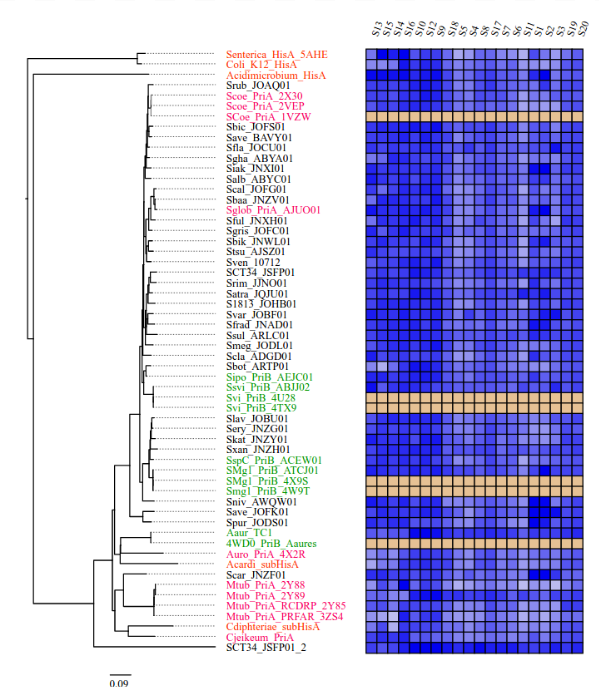
\includegraphics[angle = 0,scale = 0.6]{chapter2/PriAHeatPot.png}
  \caption[Heat Plot PriA Streptomyces vs other subtrates]{\normalsize{Heat Plot PriA Streptomyces vs other subtrates}}
  \label{fig:PriADocking}
  \end{figure}
  
  Docker simulation were calculated for Streptomyces enzymes\\
  Genome size vs Total antismash cluster coloured by order
  
  \begin{figure}[h!tbp]
  \centering
  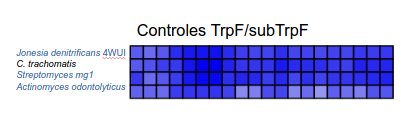
\includegraphics[angle = 0,scale = 0.6]{chapter2/TrpFHeatPlot.png}
  \caption[Heat Plot TrpF Streptomyces vs other subtrates]{\normalsize{Heat Plot TrpF Streptomyces vs other subtrates}}
  \label{fig:TrpFDocking}
  \end{figure}
  
  \TeX~is the best way to typeset mathematics. Donald Knuth designed
  \TeX~when he got frustrated at how long it was taking the typesetters to
  finish his book, which contained a lot of mathematics. One nice feature
  of \emph{R Markdown} is its ability to read \LaTeX~code directly.
  
  If you are doing a thesis that will involve lots of math, you will want
  to read the following section which has been commented out. If you're
  not going to use math, skip over or delete this next commented section.
  
  \section{Chemistry 101: Symbols}\label{chemistry-101-symbols}
  
  Chemical formulas will look best if they are not italicized. Get around
  math mode's automatic italicizing in \LaTeX~by using the argument
  \texttt{\$\textbackslash{}mathrm\{formula\ here\}\$}, with your formula
  inside the curly brackets. (Notice the use of the backticks here which
  enclose text that acts as code.)
  
  So, \(\mathrm{Fe_2^{2+}Cr_2O_4}\) is written
  \texttt{\$\textbackslash{}mathrm\{Fe\_2\^{}\{2+\}Cr\_2O\_4\}\$}.
  
  \noindent Exponent or Superscript: \(\mathrm{O^-}\)
  
  \noindent Subscript: \(\mathrm{CH_4}\)
  
  To stack numbers or letters as in \(\mathrm{Fe_2^{2+}}\), the subscript
  is defined first, and then the superscript is defined.
  
  \noindent Angstrom: \({\AA}\)
  
  \noindent Bullet: CuCl \(\bullet\) \(\mathrm{7H_{2}O}\)
  
  \noindent Double Dagger: \(\ddag\)
  
  \noindent Delta: \(\Delta\)
  
  \noindent Reaction Arrows: \(\longrightarrow\) or
  \(\xrightarrow{solution}\)
  
  \noindent Resonance Arrows: \(\leftrightarrow\)
  
  \noindent Reversible Reaction Arrows: \(\rightleftharpoons\) or
  \(\xrightleftharpoons[ ]{solution}\) (the latter requires the
  \texttt{chemarr} \LaTeX~package which is automatically loaded in this
  template)
  
  \subsection{Typesetting reactions}\label{typesetting-reactions}
  
  You may wish to put your reaction in a figure environment, which means
  that \LaTeX~will place the reaction where it fits and you can have a
  figure caption. You'll see further description of this \textbf{R}
  \texttt{label} function in \protect\hyperlink{refux5flabels}{}. (Note
  the use of the double backslash here as well as the
  \texttt{echo\ =\ FALSE} which hides the code from the output.)
  
  \begin{figure}[h!tbp]
  \begin{center}
  $\mathrm{C_6H_{12}O_6  + 6O_2} \longrightarrow \mathrm{6CO_2 + 6H_2O}$
  \caption{Combustion of glucose}
  \label{fig:comb-gluc}
  \end{center}
  \end{figure}
  
  \subsection{Other examples of
  reactions}\label{other-examples-of-reactions}
  
  \(\mathrm{NH_4Cl_{(s)}}\) \(\rightleftharpoons\)
  \(\mathrm{NH_{3(g)}+HCl_{(g)}}\)
  
  \noindent \(\mathrm{MeCH_2Br + Mg}\) \(\xrightarrow[below]{above}\)
  \(\mathrm{MeCH_2\bullet Mg \bullet Br}\)
  
  \section{Physics}\label{physics}
  
  Many of the symbols you will need can be found on the math page
  \url{http://web.reed.edu/cis/help/latex/math.html} and the Comprehensive
  \LaTeX~Symbol Guide
  (\url{http://mirror.utexas.edu/ctan/info/symbols/comprehensive/symbols-letter.pdf}).
  
  \section{Biology}\label{biology}
  
  You will probably find the resources at
  \url{http://www.lecb.ncifcrf.gov/~toms/latex.html} helpful, particularly
  the links to bsts for various journals. You may also be interested in
  TeXShade for nucleotide typesetting
  (\url{http://homepages.uni-tuebingen.de/beitz/txe.html}). Be sure to
  read the proceeding chapter on graphics and tables.
  
  \begin{Shaded}
  \begin{Highlighting}[]
  \KeywordTok{sessionInfo}\NormalTok{()}
  \end{Highlighting}
  \end{Shaded}
  
  \begin{verbatim}
  R version 3.3.2 (2016-10-31)
  Platform: x86_64-pc-linux-gnu (64-bit)
  Running under: Ubuntu 14.04.5 LTS
  
  locale:
   [1] LC_CTYPE=en_US.UTF-8          LC_NUMERIC=C                 
   [3] LC_TIME=es_MX.UTF-8           LC_COLLATE=en_US.UTF-8       
   [5] LC_MONETARY=es_MX.UTF-8       LC_MESSAGES=en_US.UTF-8      
   [7] LC_PAPER=es_MX.UTF-8          LC_NAME=es_MX.UTF-8          
   [9] LC_ADDRESS=es_MX.UTF-8        LC_TELEPHONE=es_MX.UTF-8     
  [11] LC_MEASUREMENT=es_MX.UTF-8    LC_IDENTIFICATION=es_MX.UTF-8
  
  attached base packages:
  [1] parallel  stats     graphics  grDevices utils     datasets  methods  
  [8] base     
  
  other attached packages:
   [1] xlsx_0.5.7          xlsxjars_0.6.1      rJava_0.9-8        
   [4] scales_0.4.1        Biobase_2.34.0      BiocGenerics_0.20.0
   [7] genstats_0.1.02     RColorBrewer_1.1-2  reshape_0.8.6      
  [10] plyr_1.8.4          knitr_1.15.1        ggplot2_2.2.1      
  [13] dplyr_0.5.0         ape_4.0             reedtemplates_0.1  
  [16] devtools_1.12.0    
  
  loaded via a namespace (and not attached):
   [1] Rcpp_0.12.9      highr_0.6        tools_3.3.2      digest_0.6.12   
   [5] evaluate_0.10    memoise_1.0.0    tibble_1.2       gtable_0.2.0    
   [9] nlme_3.1-131     lattice_0.20-34  DBI_0.5-1        yaml_2.1.14     
  [13] withr_1.0.2      stringr_1.1.0    rprojroot_1.2    grid_3.3.2      
  [17] R6_2.2.0         rmarkdown_1.3    magrittr_1.5     backports_1.0.5 
  [21] htmltools_0.3.5  assertthat_0.1   colorspace_1.3-2 labeling_0.3    
  [25] stringi_1.1.2    lazyeval_0.2.0   munsell_0.4.3   
  \end{verbatim}
  
  \hypertarget{refux5flabels}{\chapter{Archaea EvoMining
  Results}\label{refux5flabels}}
  
  During the decade between 1970 and 1980, Archaea was recognized as new
  life domain, a kingdom different from Bacteria and Eucarya in an
  exciting first great application of 16S
  phylogeny{[}\protect\hyperlink{ref-woeseux5fphylogeneticux5f1977}{115}{]}
  . Main differences between this kingdoms are that Archaeal DNA is not
  arranged in a nucleus as in Eucarya and Archaeal celular walls are not
  composed from peptidoglycans as in Bacteria. Archaeal proteins may be
  higlhy valuable to biotechnology industry for their great stability due
  to extreme temperature, PH and salt content conditions on Archeal
  habitats. Despite no Archaeal Natural products biosynthetic gene
  clusters (BGC's) has been reported on MiBIG, Archaea do have BGC's, some
  of them seems to be acquired by horizontal gene transfer (HGT) like
  methano nrps \{search reference\}. Other Archeal natural products known
  are archaeosins, Diketopiperazines, Acyl Homoserine Lactones,
  Exopolysaccharides, Carotenoids, Biosurfactants, Phenazines and Organic
  Solutes but this knowledge is not comparable to Bacterial BGC's
  knowledge{[}\protect\hyperlink{ref-charlesworthux5funtappedux5f2015}{99}{]}.
  
  Natural products biosynthetic gene clusters search is actually performed
  using either \emph{high-confidence/low-novelty or
  low-confidence/high-novelty} bioinformatic approaches
  {[}\protect\hyperlink{ref-medemaux5fcomputationalux5f2015}{50}{]}. High
  confidence methods compares query sequences with previously known BGC's
  such as nrps or PKS, examples of this algorithms are antiSMASH and
  clusterfinder {[}\textbf{???}?{]}. EvoMining searches on expansions from
  central metabolic pathways enzyme families, it has been classified as
  low confidence/high novelty method. EvoMining has proved useful on
  Actinobacteria phylum where its use lead to Arseno-compounds discovery
  {[}\protect\hyperlink{ref-cruz-moralesux5fphylogenomicux5f2016}{65}{]}.
  Also on Actinobacteria antiSMASH analysis on 1245 genomes found 774
  different classes of natural products, the same analysis on 876 Archaeal
  genomes, a full kingdom, identifies only 35 BGC's classes. So either
  Archaea does not have natural products BGC's or this are not yet known.
  Next paragraph deals with a possible approach about how natural products
  BGC's can be find.
  
  Archaea resembled Bacteria in that Archaea uses horizontal gene transfer
  as a genic interchange mecanism, Archaeal genomes contains operons
  {[}\protect\hyperlink{ref-howlandux5fsurprisingux5f2000}{118}{]} and in
  general there is introns absence\{Reference to Computational Methods for
  Understanding Bacterial and Archaeal Genomes\}. Archaeas do have
  introns, but they are mainly located on genes that encodes ribosomal and
  transfer RNA
  {[}\protect\hyperlink{ref-howlandux5fsurprisingux5f2000}{118}{]}.
  General lack of introns allows automatic genome annotation, operons gene
  organization permits functional inference to a certain degree and HGT
  contribute to expansions on Archaeal genomes. Some phylum on Archaea has
  an open pangenome, and as we will show on this chapter some Archaea has
  central pathway expansions. Enzyme families from central pathways
  expansions, open pangenome and operon organization made EvoMining
  succesful on Actinobacteria, this lead us to think that evoMining is
  suitable to analize Archaeal genomes, even more since EvoMining is a
  method oriented to use evolution and its not entirelyy based on previous
  knowledge of BGC's sequences if evolutionary logic behave on Archaea as
  on bacteria, new BGC's classes may be be found on Archaea.
  
  EvoMining is a trade off between conserved known central metabolic
  function and enough expansions divergence on sequence and on clusters to
  divergence
  
  \section{Tables}\label{tables}
  
  \begin{longtable}[c]{@{}cc@{}}
  \caption{Families on Archaeabacteria \label{tab:inher}}\tabularnewline
  \toprule
  Factors & Correlation between Parents \& Child\tabularnewline
  \midrule
  \endfirsthead
  \toprule
  Factors & Correlation between Parents \& Child\tabularnewline
  \midrule
  \endhead
  GenomeDB & 876\tabularnewline
  Phylum & 12\tabularnewline
  Order & 23\tabularnewline
  \bottomrule
  \end{longtable}
  
  \clearpage
  
  First lets investigate if Archaea has expansions on families within
  central metabolic routes. Since main metabolic pathways are shared
  between Bacteria and Archaea makes sense to assemble Archeal EvoMining
  central database by using orthologous from Actinobacteria evoMining
  central pathways.
  
  \subsection{Expansions BoxPlot by metabolic
  family}\label{expansions-boxplot-by-metabolic-family}
  
  \begin{Shaded}
  \begin{Highlighting}[]
  \KeywordTok{label}\NormalTok{(}\DataTypeTok{path =} \StringTok{"chapter3/expansion_plotArchaeas.pdf"}\NormalTok{, }\DataTypeTok{caption =} \StringTok{"Expansions Boxplot"}\NormalTok{,}\DataTypeTok{label =} \StringTok{"Archaea_expansion_boxplot"}\NormalTok{, }\DataTypeTok{type =} \StringTok{"figure"}\NormalTok{,}\DataTypeTok{scale=}\StringTok{".7"}\NormalTok{)}
  \end{Highlighting}
  \end{Shaded}
  
  \begin{figure}[h!tbp]
  \centering
  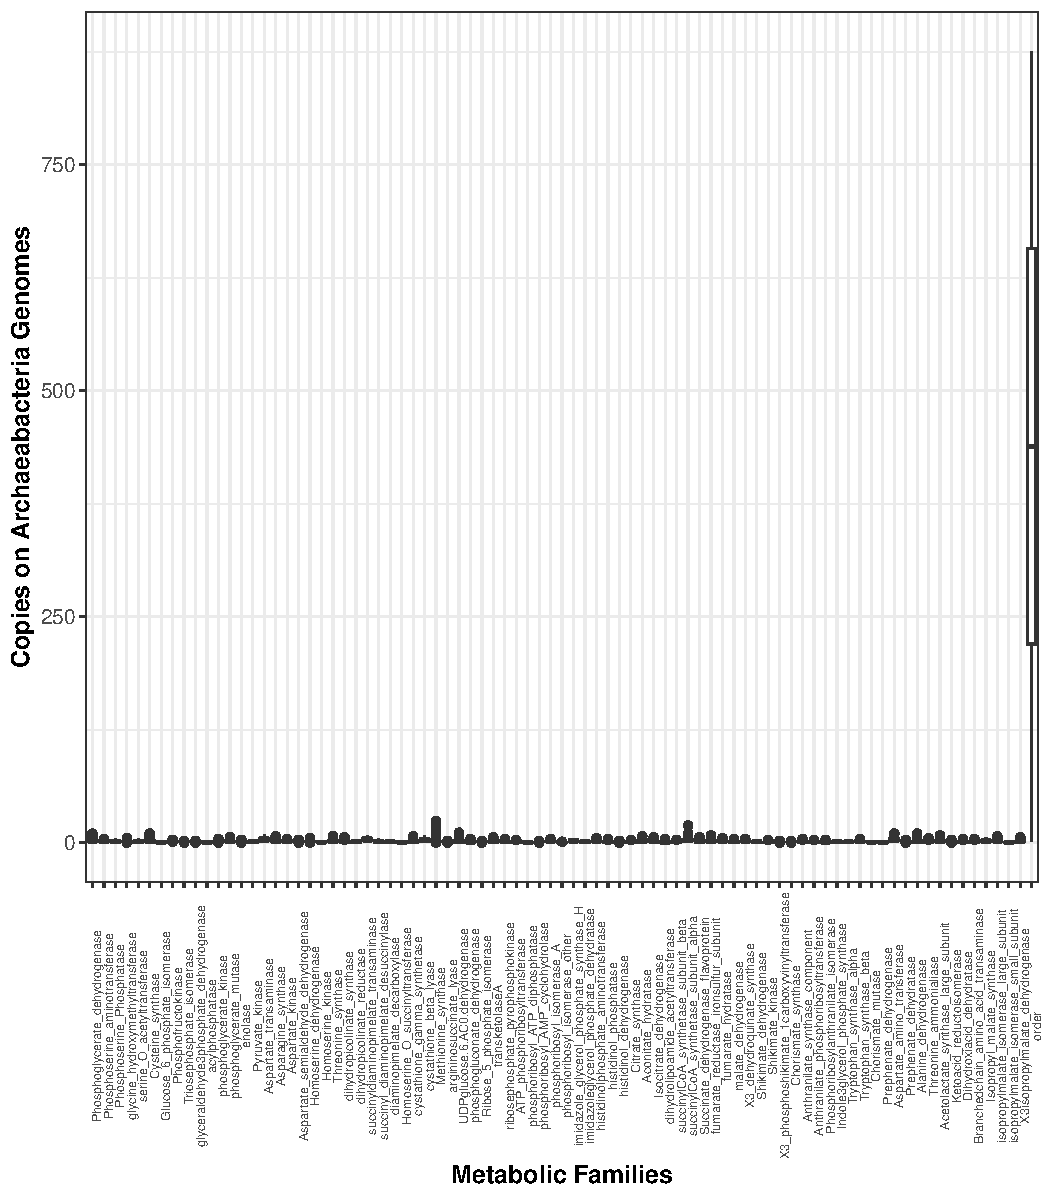
\includegraphics[angle = 0,scale = .7]{chapter3/expansion_plotArchaeas.pdf}
  \caption[Expansions Boxplot]{\normalsize{Expansions Boxplot}}
  \label{fig:Archaea_expansion_boxplot}
  \end{figure}
  
  Here is a reference to the expansion boxplot:
  \autoref{fig:Archaea_expansion_boxplot}.\\
  \clearpage 
  
  \subsection{Expansions BoxPlot by metabolic family by
  phylum}\label{expansions-boxplot-by-metabolic-family-by-phylum}
  
  \begin{Shaded}
  \begin{Highlighting}[]
  \CommentTok{#+ geom_jitter()}
  \CommentTok{#aes(fill = factor(vs))}
  
  \NormalTok{ArchaeasTotalBP.m<-}\KeywordTok{merge}\NormalTok{(ArchaeasHeatPlot,ArchaeasTaxa,}\DataTypeTok{by.x=}\StringTok{"RastId"}\NormalTok{,}\DataTypeTok{by.y=}\StringTok{"RastId"}\NormalTok{) ## works as expected}
  \NormalTok{ArchaeasHeatPlotBP.m <-}\StringTok{ }\KeywordTok{melt}\NormalTok{(ArchaeasTotalBP.m,}\DataTypeTok{id =}\KeywordTok{c}\NormalTok{(}\StringTok{"RastId"}\NormalTok{,}\StringTok{"Name"}\NormalTok{,}\StringTok{"SuperPhylum"}\NormalTok{,}\StringTok{"Phylum"}\NormalTok{,}\StringTok{"Class"}\NormalTok{,}\StringTok{"Order"}\NormalTok{,}\StringTok{"Family"}\NormalTok{,}\StringTok{"RastNo"}\NormalTok{,}\StringTok{"Size"}\NormalTok{,}\StringTok{"Contigs"}\NormalTok{))}
  \NormalTok{ArchaeasHeatPlotBP.m<-}\KeywordTok{subset}\NormalTok{(ArchaeasHeatPlotBP.m,variable!=}\StringTok{"TOTAL"}\NormalTok{) ## works as expected}
  \NormalTok{ArchaeasHeatPlotBP.m<-}\KeywordTok{subset}\NormalTok{(ArchaeasHeatPlotBP.m,variable!=}\StringTok{"TOTAL"}\NormalTok{) ## works as expected}
  
  \NormalTok{## Each metabolic pathway se parte por phylum coloreado por order}
  
  \CommentTok{#3PGA_AMINOACIDS}
  \CommentTok{#Glycolysis}
  \CommentTok{#OXALACETATE_AMINOACIDS}
  \CommentTok{#R5P_AMINOACIDS}
  \CommentTok{#TCA}
  \CommentTok{#E4P_AMINO_ACIDS}
  \CommentTok{#PYR_THR_AA}
  
  \NormalTok{## Genome size}
  \KeywordTok{ggplot}\NormalTok{(ArchaeasHeatPlotBP.m, }\KeywordTok{aes}\NormalTok{(}\DataTypeTok{x=}\NormalTok{ArchaeasHeatPlotBP.m$Phylum, }\DataTypeTok{y=}\NormalTok{ArchaeasHeatPlotBP.m$Size))+}\StringTok{ }\KeywordTok{geom_boxplot}\NormalTok{() +}\KeywordTok{theme}\NormalTok{(}\DataTypeTok{plot.title =} \KeywordTok{element_text}\NormalTok{(}\DataTypeTok{size =} \DecValTok{14}\NormalTok{, }\DataTypeTok{face =} \StringTok{"bold"}\NormalTok{), }\DataTypeTok{text =} \KeywordTok{element_text}\NormalTok{(}\DataTypeTok{size =} \DecValTok{12}\NormalTok{), }\DataTypeTok{axis.title =} \KeywordTok{element_text}\NormalTok{(}\DataTypeTok{face=}\StringTok{"bold"}\NormalTok{), }\DataTypeTok{axis.text.x=}\KeywordTok{element_text}\NormalTok{(}\DataTypeTok{angle =} \DecValTok{90}\NormalTok{,}\DataTypeTok{size =} \DecValTok{6}\NormalTok{), }\DataTypeTok{legend.position =} \StringTok{"bottom"}\NormalTok{)+}\StringTok{ }\KeywordTok{labs}\NormalTok{(}\DataTypeTok{x =} \StringTok{"Copies on Archaeabacteria taxonomic groups"}\NormalTok{, }\DataTypeTok{y =} \StringTok{"Genome size"}\NormalTok{,}\DataTypeTok{text =} \KeywordTok{element_text}\NormalTok{(}\DataTypeTok{size=}\DecValTok{12}\NormalTok{))+}\KeywordTok{theme_bw}\NormalTok{()}
  \end{Highlighting}
  \end{Shaded}
  
  \begin{center}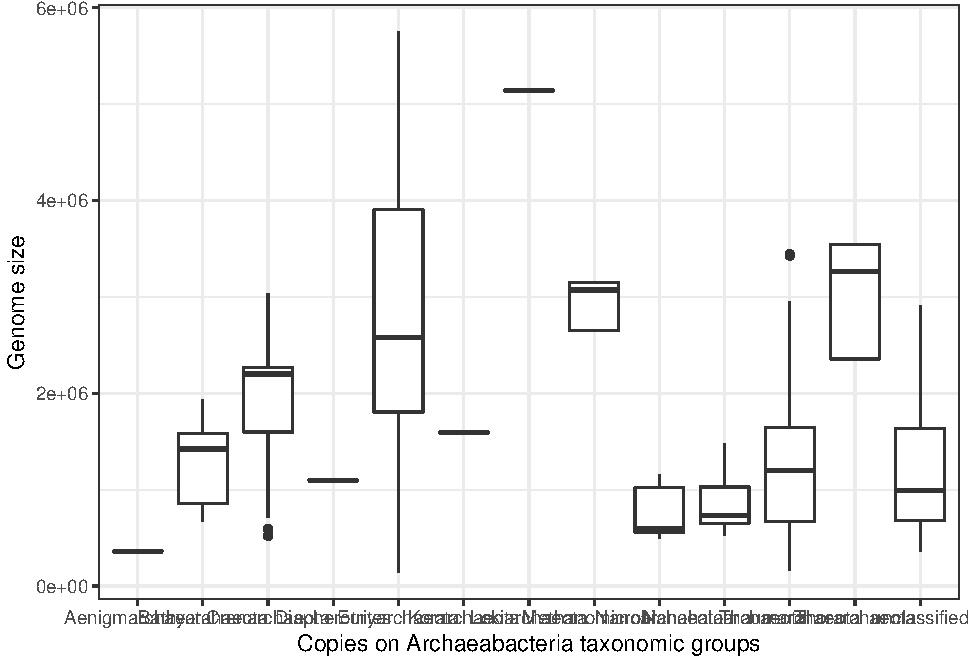
\includegraphics{tesis_files/figure-latex/ArcheaeBoxPlotByPhylum-1} \end{center}
  
  \begin{Shaded}
  \begin{Highlighting}[]
  \CommentTok{#+ geom_jitter(aes(color=ArchaeasHeatPlotBP.m$Phylum))}
  
  
  \NormalTok{## Halobacteria}
  \NormalTok{MetFam_BP.m=}\KeywordTok{subset}\NormalTok{(ArchaeasHeatPlotBP.m,Phylum==}\StringTok{"Euryarchaeota"}\NormalTok{)}
  \KeywordTok{ggplot}\NormalTok{(MetFam_BP.m, }\KeywordTok{aes}\NormalTok{(}\DataTypeTok{x=}\NormalTok{MetFam_BP.m$Order, }\DataTypeTok{y=}\NormalTok{MetFam_BP.m$Size))+}\StringTok{ }\KeywordTok{geom_boxplot}\NormalTok{() +}\KeywordTok{theme}\NormalTok{(}\DataTypeTok{plot.title =} \KeywordTok{element_text}\NormalTok{(}\DataTypeTok{size =} \DecValTok{14}\NormalTok{, }\DataTypeTok{face =} \StringTok{"bold"}\NormalTok{), }\DataTypeTok{text =} \KeywordTok{element_text}\NormalTok{(}\DataTypeTok{size =} \DecValTok{12}\NormalTok{), }\DataTypeTok{axis.title =} \KeywordTok{element_text}\NormalTok{(}\DataTypeTok{face=}\StringTok{"bold"}\NormalTok{), }\DataTypeTok{axis.text.x=}\KeywordTok{element_text}\NormalTok{(}\DataTypeTok{angle =} \DecValTok{90}\NormalTok{,}\DataTypeTok{size =} \DecValTok{10}\NormalTok{), }\DataTypeTok{legend.position =} \StringTok{"bottom"}\NormalTok{)+}\StringTok{ }\KeywordTok{labs}\NormalTok{(}\DataTypeTok{x =} \StringTok{"Halobacteria orders size taxonomic groups"}\NormalTok{, }\DataTypeTok{y =} \StringTok{"Genome size"}\NormalTok{,}\DataTypeTok{text =} \KeywordTok{element_text}\NormalTok{(}\DataTypeTok{size=}\DecValTok{12}\NormalTok{)) +}\StringTok{ }\KeywordTok{geom_jitter}\NormalTok{(}\KeywordTok{aes}\NormalTok{(}\DataTypeTok{color=}\NormalTok{Family))}
  \end{Highlighting}
  \end{Shaded}
  
  \begin{center}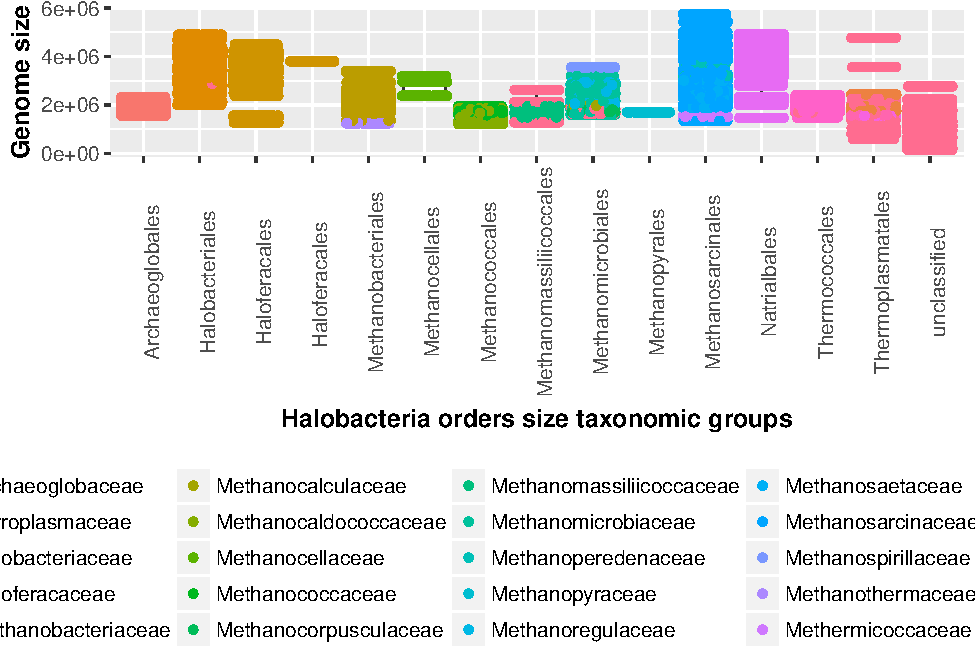
\includegraphics{tesis_files/figure-latex/ArcheaeBoxPlotByPhylum-2} \end{center}
  
  \begin{Shaded}
  \begin{Highlighting}[]
  \CommentTok{#MetFam_BP.m=subset(ArchaeasHeatPlotBP.m,Family=="Methanosarcinaceae")}
  \CommentTok{#ggplot(MetFam_BP.m, aes(x=MetFam_BP.m$Size, y=MetFam_BP.m$value))}
  \CommentTok{#+theme(plot.title = element_text(size = 14, face = "bold"), text = element_text(size = 12), axis.title = element_text(face="bold"), axis.text.x=element_text(angle = 90,size = 10), legend.position = "bottom")+ labs(x = "Copies on Archaeabacteria taxonomic groups", y = "Genome size",text = element_text(size=12)) }
  
  
    \CommentTok{#geom_jitter(aes(color=ArchaeasHeatPlotBP.m$Phylum))# + facet_grid(. ~ Phylum)+theme_bw()}
  
  
  \NormalTok{## Metabolic Pathways}
  \NormalTok{MetFam=}\KeywordTok{subset}\NormalTok{(ArchaeasCentral,Pathway==}\StringTok{"PPP"}\NormalTok{)}
  \NormalTok{MetFam_BP.m=ArchaeasHeatPlotBP.m[ArchaeasHeatPlotBP.m$variable %in%}\StringTok{ }\NormalTok{MetFam$Enzyme,]}
  \KeywordTok{ggplot}\NormalTok{(MetFam_BP.m, }\KeywordTok{aes}\NormalTok{(}\DataTypeTok{x=}\NormalTok{MetFam_BP.m$variable, }\DataTypeTok{y=}\NormalTok{MetFam_BP.m$value, }\DataTypeTok{fill=}\NormalTok{Order))+}\StringTok{ }\KeywordTok{labs}\NormalTok{(}\DataTypeTok{x =} \StringTok{"Metabolic PPP Families"}\NormalTok{, }\DataTypeTok{y =} \StringTok{"Copies on Archaeabacteria Genomes"}\NormalTok{,}\DataTypeTok{text =} \KeywordTok{element_text}\NormalTok{(}\DataTypeTok{size=}\DecValTok{12}\NormalTok{)) +}\StringTok{ }\KeywordTok{geom_boxplot}\NormalTok{() +}\StringTok{ }\KeywordTok{facet_grid}\NormalTok{(. ~}\StringTok{ }\NormalTok{Phylum)+}\KeywordTok{theme_bw}\NormalTok{() +}\KeywordTok{theme}\NormalTok{(}\DataTypeTok{plot.title =} \KeywordTok{element_text}\NormalTok{(}\DataTypeTok{size =} \DecValTok{14}\NormalTok{, }\DataTypeTok{face =} \StringTok{"bold"}\NormalTok{), }\DataTypeTok{text =} \KeywordTok{element_text}\NormalTok{(}\DataTypeTok{size =} \DecValTok{12}\NormalTok{), }\DataTypeTok{axis.title =} \KeywordTok{element_text}\NormalTok{(}\DataTypeTok{face=}\StringTok{"bold"}\NormalTok{), }\DataTypeTok{axis.text.x=}\KeywordTok{element_text}\NormalTok{(}\DataTypeTok{angle =} \DecValTok{90}\NormalTok{,}\DataTypeTok{size =} \DecValTok{6}\NormalTok{), }\DataTypeTok{legend.position =} \StringTok{"bottom"}\NormalTok{)}
  \end{Highlighting}
  \end{Shaded}
  
  \begin{center}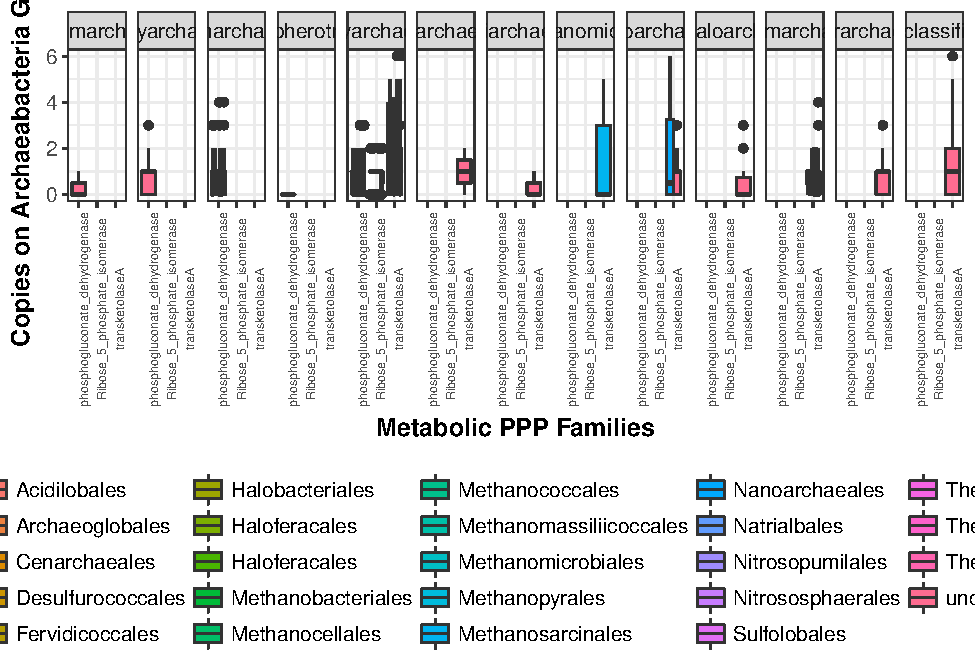
\includegraphics{tesis_files/figure-latex/ArcheaeBoxPlotByPhylum-3} \end{center}
  
  \begin{Shaded}
  \begin{Highlighting}[]
  \CommentTok{#+ geom_jitter(aes(color=MetFam_BP.m$Phylum))       }
  
  \NormalTok{MetFam=}\KeywordTok{subset}\NormalTok{(ArchaeasCentral,Pathway==}\StringTok{"3PGA_AMINOACIDS"}\NormalTok{)}
  \NormalTok{MetFam_BP.m=ArchaeasHeatPlotBP.m[ArchaeasHeatPlotBP.m$variable %in%}\StringTok{ }\NormalTok{MetFam$Enzyme,]}
  \KeywordTok{ggplot}\NormalTok{(MetFam_BP.m, }\KeywordTok{aes}\NormalTok{(}\DataTypeTok{x=}\NormalTok{MetFam_BP.m$variable, }\DataTypeTok{y=}\NormalTok{MetFam_BP.m$value, }\DataTypeTok{fill=}\NormalTok{Order))+}\StringTok{ }\KeywordTok{labs}\NormalTok{(}\DataTypeTok{x =} \StringTok{"Metabolic PGA_AMINOACIDS Families"}\NormalTok{, }\DataTypeTok{y =} \StringTok{"Copies on Archaeabacteria Genomes"}\NormalTok{,}\DataTypeTok{text =} \KeywordTok{element_text}\NormalTok{(}\DataTypeTok{size=}\DecValTok{12}\NormalTok{)) +}\StringTok{ }\KeywordTok{geom_boxplot}\NormalTok{() +}\StringTok{ }\KeywordTok{facet_grid}\NormalTok{(. ~}\StringTok{ }\NormalTok{Phylum)+}\KeywordTok{theme_bw}\NormalTok{()+}\KeywordTok{theme}\NormalTok{(}\DataTypeTok{plot.title =} \KeywordTok{element_text}\NormalTok{(}\DataTypeTok{size =} \DecValTok{14}\NormalTok{, }\DataTypeTok{face =} \StringTok{"bold"}\NormalTok{), }\DataTypeTok{text =} \KeywordTok{element_text}\NormalTok{(}\DataTypeTok{size =} \DecValTok{12}\NormalTok{), }\DataTypeTok{axis.title =} \KeywordTok{element_text}\NormalTok{(}\DataTypeTok{face=}\StringTok{"bold"}\NormalTok{), }\DataTypeTok{axis.text.x=}\KeywordTok{element_text}\NormalTok{(}\DataTypeTok{angle =} \DecValTok{90}\NormalTok{,}\DataTypeTok{size =} \DecValTok{6}\NormalTok{), }\DataTypeTok{legend.position =} \StringTok{"bottom"}\NormalTok{)}
  \end{Highlighting}
  \end{Shaded}
  
  \begin{center}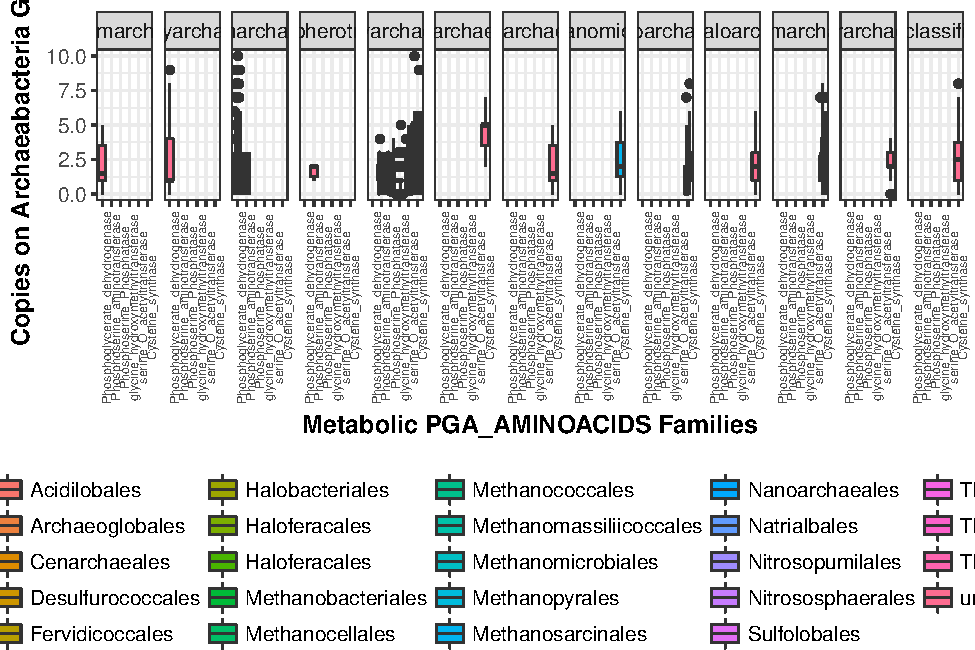
\includegraphics{tesis_files/figure-latex/ArcheaeBoxPlotByPhylum-4} \end{center}
  
  \begin{Shaded}
  \begin{Highlighting}[]
  \CommentTok{#+ geom_jitter(aes(color=MetFam_BP.m$Phylum))}
  
  \NormalTok{MetFam=}\KeywordTok{subset}\NormalTok{(ArchaeasCentral,Pathway==}\StringTok{"Glycolysis"}\NormalTok{)}
  \NormalTok{MetFam_BP.m=ArchaeasHeatPlotBP.m[ArchaeasHeatPlotBP.m$variable %in%}\StringTok{ }\NormalTok{MetFam$Enzyme,]}
  \KeywordTok{ggplot}\NormalTok{(MetFam_BP.m, }\KeywordTok{aes}\NormalTok{(}\DataTypeTok{x=}\NormalTok{MetFam_BP.m$variable, }\DataTypeTok{y=}\NormalTok{MetFam_BP.m$value, }\DataTypeTok{fill=}\NormalTok{Order))+}\StringTok{ }\KeywordTok{labs}\NormalTok{(}\DataTypeTok{x =} \StringTok{"Metabolic Glycolysis Families"}\NormalTok{, }\DataTypeTok{y =} \StringTok{"Copies on Archaeabacteria Genomes"}\NormalTok{,}\DataTypeTok{text =} \KeywordTok{element_text}\NormalTok{(}\DataTypeTok{size=}\DecValTok{12}\NormalTok{)) +}\StringTok{ }\KeywordTok{geom_boxplot}\NormalTok{() +}\StringTok{ }\KeywordTok{facet_grid}\NormalTok{(. ~}\StringTok{ }\NormalTok{Phylum)+}\KeywordTok{theme_bw}\NormalTok{()+}\KeywordTok{theme}\NormalTok{(}\DataTypeTok{plot.title =} \KeywordTok{element_text}\NormalTok{(}\DataTypeTok{size =} \DecValTok{14}\NormalTok{, }\DataTypeTok{face =} \StringTok{"bold"}\NormalTok{), }\DataTypeTok{text =} \KeywordTok{element_text}\NormalTok{(}\DataTypeTok{size =} \DecValTok{12}\NormalTok{), }\DataTypeTok{axis.title =} \KeywordTok{element_text}\NormalTok{(}\DataTypeTok{face=}\StringTok{"bold"}\NormalTok{), }\DataTypeTok{axis.text.x=}\KeywordTok{element_text}\NormalTok{(}\DataTypeTok{angle =} \DecValTok{90}\NormalTok{,}\DataTypeTok{size =} \DecValTok{6}\NormalTok{), }\DataTypeTok{legend.position =} \StringTok{"bottom"}\NormalTok{)}
  \end{Highlighting}
  \end{Shaded}
  
  \begin{center}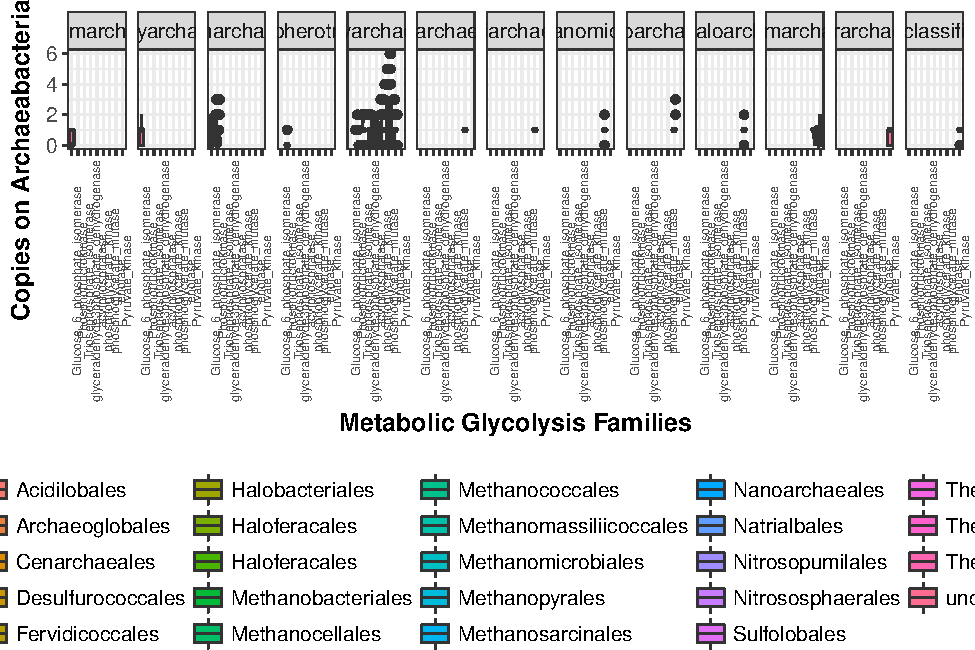
\includegraphics{tesis_files/figure-latex/ArcheaeBoxPlotByPhylum-5} \end{center}
  
  \begin{Shaded}
  \begin{Highlighting}[]
  \CommentTok{#+ geom_jitter(aes(color=MetFam_BP.m$Phylum))}
  
  \NormalTok{MetFam=}\KeywordTok{subset}\NormalTok{(ArchaeasCentral,Pathway==}\StringTok{"OXALACETATE_AMINOACIDS"}\NormalTok{)}
  \NormalTok{MetFam_BP.m=ArchaeasHeatPlotBP.m[ArchaeasHeatPlotBP.m$variable %in%}\StringTok{ }\NormalTok{MetFam$Enzyme,]}
  \KeywordTok{ggplot}\NormalTok{(MetFam_BP.m, }\KeywordTok{aes}\NormalTok{(}\DataTypeTok{x=}\NormalTok{MetFam_BP.m$variable, }\DataTypeTok{y=}\NormalTok{MetFam_BP.m$value, }\DataTypeTok{fill=}\NormalTok{Order))+}\StringTok{ }\KeywordTok{labs}\NormalTok{(}\DataTypeTok{x =} \StringTok{"Metabolic OXALACETATE_AMINOACIDS Families"}\NormalTok{, }\DataTypeTok{y =} \StringTok{"Copies on Archaeabacteria Genomes"}\NormalTok{,}\DataTypeTok{text =} \KeywordTok{element_text}\NormalTok{(}\DataTypeTok{size=}\DecValTok{12}\NormalTok{)) +}\StringTok{ }\KeywordTok{geom_boxplot}\NormalTok{() +}\StringTok{ }\KeywordTok{facet_grid}\NormalTok{(. ~}\StringTok{ }\NormalTok{Phylum)+}\KeywordTok{theme_bw}\NormalTok{()+}\KeywordTok{theme}\NormalTok{(}\DataTypeTok{plot.title =} \KeywordTok{element_text}\NormalTok{(}\DataTypeTok{size =} \DecValTok{14}\NormalTok{, }\DataTypeTok{face =} \StringTok{"bold"}\NormalTok{), }\DataTypeTok{text =} \KeywordTok{element_text}\NormalTok{(}\DataTypeTok{size =} \DecValTok{12}\NormalTok{), }\DataTypeTok{axis.title =} \KeywordTok{element_text}\NormalTok{(}\DataTypeTok{face=}\StringTok{"bold"}\NormalTok{), }\DataTypeTok{axis.text.x=}\KeywordTok{element_text}\NormalTok{(}\DataTypeTok{angle =} \DecValTok{90}\NormalTok{,}\DataTypeTok{size =} \DecValTok{6}\NormalTok{), }\DataTypeTok{legend.position =} \StringTok{"bottom"}\NormalTok{)}
  \end{Highlighting}
  \end{Shaded}
  
  \begin{center}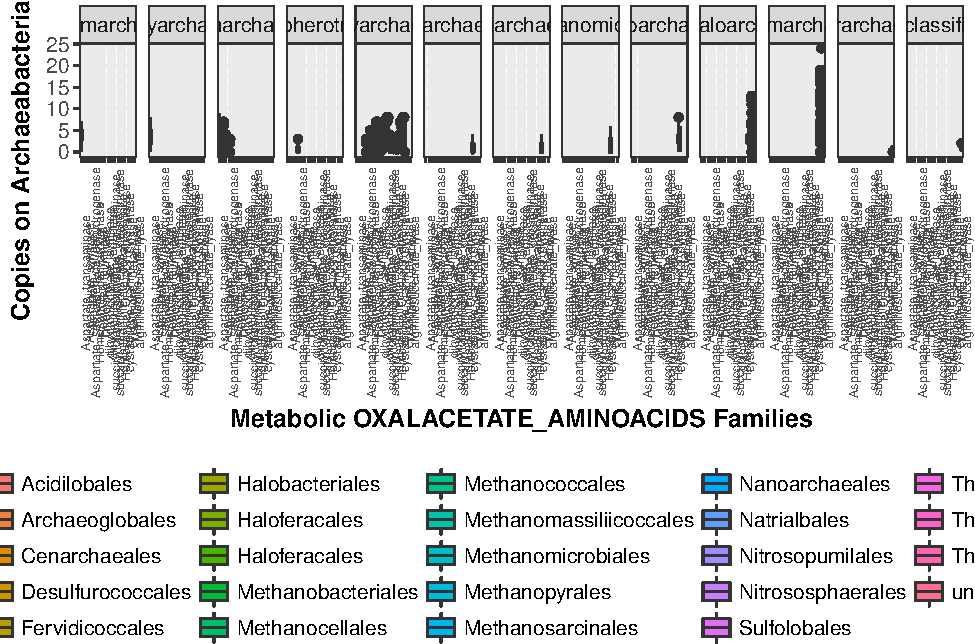
\includegraphics{tesis_files/figure-latex/ArcheaeBoxPlotByPhylum-6} \end{center}
  
  \begin{Shaded}
  \begin{Highlighting}[]
  \CommentTok{#+ geom_jitter(aes(color=MetFam_BP.m$Phylum))}
  
  \NormalTok{MetFam=}\KeywordTok{subset}\NormalTok{(ArchaeasCentral,Pathway==}\StringTok{"R5P_AMINOACIDS"}\NormalTok{)}
  \NormalTok{MetFam_BP.m=ArchaeasHeatPlotBP.m[ArchaeasHeatPlotBP.m$variable %in%}\StringTok{ }\NormalTok{MetFam$Enzyme,]}
  \KeywordTok{ggplot}\NormalTok{(MetFam_BP.m, }\KeywordTok{aes}\NormalTok{(}\DataTypeTok{x=}\NormalTok{MetFam_BP.m$variable, }\DataTypeTok{y=}\NormalTok{MetFam_BP.m$value, }\DataTypeTok{fill=}\NormalTok{Order))+}\StringTok{ }\KeywordTok{labs}\NormalTok{(}\DataTypeTok{x =} \StringTok{"Metabolic R5P_AMINOACIDS Families"}\NormalTok{, }\DataTypeTok{y =} \StringTok{"Copies on Archaeabacteria Genomes"}\NormalTok{,}\DataTypeTok{text =} \KeywordTok{element_text}\NormalTok{(}\DataTypeTok{size=}\DecValTok{12}\NormalTok{)) +}\StringTok{ }\KeywordTok{geom_boxplot}\NormalTok{() +}\StringTok{ }\KeywordTok{facet_grid}\NormalTok{(. ~}\StringTok{ }\NormalTok{Phylum)+}\KeywordTok{theme_bw}\NormalTok{()+}\KeywordTok{theme}\NormalTok{(}\DataTypeTok{plot.title =} \KeywordTok{element_text}\NormalTok{(}\DataTypeTok{size =} \DecValTok{14}\NormalTok{, }\DataTypeTok{face =} \StringTok{"bold"}\NormalTok{), }\DataTypeTok{text =} \KeywordTok{element_text}\NormalTok{(}\DataTypeTok{size =} \DecValTok{12}\NormalTok{), }\DataTypeTok{axis.title =} \KeywordTok{element_text}\NormalTok{(}\DataTypeTok{face=}\StringTok{"bold"}\NormalTok{), }\DataTypeTok{axis.text.x=}\KeywordTok{element_text}\NormalTok{(}\DataTypeTok{angle =} \DecValTok{90}\NormalTok{,}\DataTypeTok{size =} \DecValTok{6}\NormalTok{), }\DataTypeTok{legend.position =} \StringTok{"bottom"}\NormalTok{)}
  \end{Highlighting}
  \end{Shaded}
  
  \begin{center}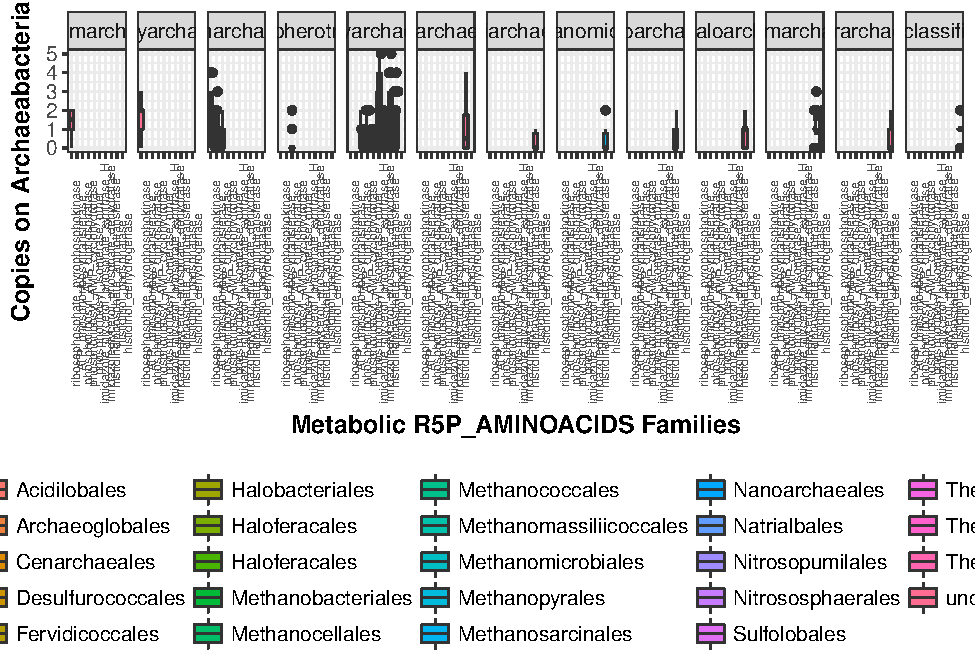
\includegraphics{tesis_files/figure-latex/ArcheaeBoxPlotByPhylum-7} \end{center}
  
  \begin{Shaded}
  \begin{Highlighting}[]
   \CommentTok{#+ geom_jitter(aes(color=MetFam_BP.m$Phylum))}
  
  \CommentTok{#}
  \NormalTok{MetFam=}\KeywordTok{subset}\NormalTok{(ArchaeasCentral,Pathway==}\StringTok{"TCA"}\NormalTok{)}
  \NormalTok{MetFam_BP.m=ArchaeasHeatPlotBP.m[ArchaeasHeatPlotBP.m$variable %in%}\StringTok{ }\NormalTok{MetFam$Enzyme,]}
  \KeywordTok{ggplot}\NormalTok{(MetFam_BP.m, }\KeywordTok{aes}\NormalTok{(}\DataTypeTok{x=}\NormalTok{MetFam_BP.m$variable, }\DataTypeTok{y=}\NormalTok{MetFam_BP.m$value, }\DataTypeTok{fill=}\NormalTok{Order))+}\StringTok{ }\KeywordTok{labs}\NormalTok{(}\DataTypeTok{x =} \StringTok{"Metabolic TCA Families"}\NormalTok{, }\DataTypeTok{y =} \StringTok{"Copies on Archaeabacteria Genomes"}\NormalTok{,}\DataTypeTok{text =} \KeywordTok{element_text}\NormalTok{(}\DataTypeTok{size=}\DecValTok{12}\NormalTok{)) +}\StringTok{ }\KeywordTok{geom_boxplot}\NormalTok{() +}\StringTok{ }\KeywordTok{facet_grid}\NormalTok{(. ~}\StringTok{ }\NormalTok{Phylum)+}\KeywordTok{theme_bw}\NormalTok{() +}\KeywordTok{theme}\NormalTok{(}\DataTypeTok{plot.title =} \KeywordTok{element_text}\NormalTok{(}\DataTypeTok{size =} \DecValTok{14}\NormalTok{, }\DataTypeTok{face =} \StringTok{"bold"}\NormalTok{), }\DataTypeTok{text =} \KeywordTok{element_text}\NormalTok{(}\DataTypeTok{size =} \DecValTok{12}\NormalTok{), }\DataTypeTok{axis.title =} \KeywordTok{element_text}\NormalTok{(}\DataTypeTok{face=}\StringTok{"bold"}\NormalTok{), }\DataTypeTok{axis.text.x=}\KeywordTok{element_text}\NormalTok{(}\DataTypeTok{angle =} \DecValTok{90}\NormalTok{,}\DataTypeTok{size =} \DecValTok{6}\NormalTok{), }\DataTypeTok{legend.position =} \StringTok{"bottom"}\NormalTok{)}
  \end{Highlighting}
  \end{Shaded}
  
  \begin{center}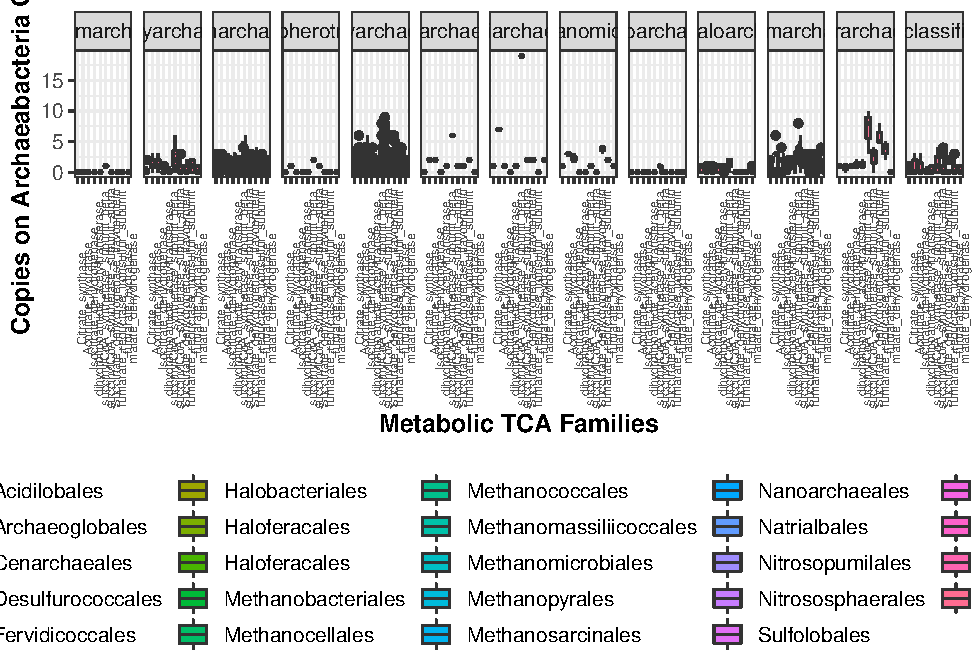
\includegraphics{tesis_files/figure-latex/ArcheaeBoxPlotByPhylum-8} \end{center}
  
  \begin{Shaded}
  \begin{Highlighting}[]
  \CommentTok{#+ geom_jitter(aes(color=MetFam_BP.m$Phylum))}
  
  \NormalTok{MetFam=}\KeywordTok{subset}\NormalTok{(ArchaeasCentral,Pathway==}\StringTok{"E4P_AMINO_ACIDS"}\NormalTok{)}
  \NormalTok{MetFam_BP.m=ArchaeasHeatPlotBP.m[ArchaeasHeatPlotBP.m$variable %in%}\StringTok{ }\NormalTok{MetFam$Enzyme,]}
  \KeywordTok{ggplot}\NormalTok{(MetFam_BP.m, }\KeywordTok{aes}\NormalTok{(}\DataTypeTok{x=}\NormalTok{MetFam_BP.m$variable, }\DataTypeTok{y=}\NormalTok{MetFam_BP.m$value, }\DataTypeTok{fill=}\NormalTok{Order))+}\StringTok{ }\KeywordTok{labs}\NormalTok{(}\DataTypeTok{x =} \StringTok{"Metabolic E4P_AMINO_ACIDS Families"}\NormalTok{, }\DataTypeTok{y =} \StringTok{"Copies on Archaeabacteria Genomes"}\NormalTok{,}\DataTypeTok{text =} \KeywordTok{element_text}\NormalTok{(}\DataTypeTok{size=}\DecValTok{12}\NormalTok{)) +}\StringTok{ }\KeywordTok{geom_boxplot}\NormalTok{() +}\StringTok{ }\KeywordTok{facet_grid}\NormalTok{(. ~}\StringTok{ }\NormalTok{Phylum)+}\KeywordTok{theme_bw}\NormalTok{() +}\KeywordTok{theme}\NormalTok{(}\DataTypeTok{plot.title =} \KeywordTok{element_text}\NormalTok{(}\DataTypeTok{size =} \DecValTok{14}\NormalTok{, }\DataTypeTok{face =} \StringTok{"bold"}\NormalTok{), }\DataTypeTok{text =} \KeywordTok{element_text}\NormalTok{(}\DataTypeTok{size =} \DecValTok{12}\NormalTok{), }\DataTypeTok{axis.title =} \KeywordTok{element_text}\NormalTok{(}\DataTypeTok{face=}\StringTok{"bold"}\NormalTok{), }\DataTypeTok{axis.text.x=}\KeywordTok{element_text}\NormalTok{(}\DataTypeTok{angle =} \DecValTok{90}\NormalTok{,}\DataTypeTok{size =} \DecValTok{6}\NormalTok{), }\DataTypeTok{legend.position =} \StringTok{"bottom"}\NormalTok{)}
  \end{Highlighting}
  \end{Shaded}
  
  \begin{center}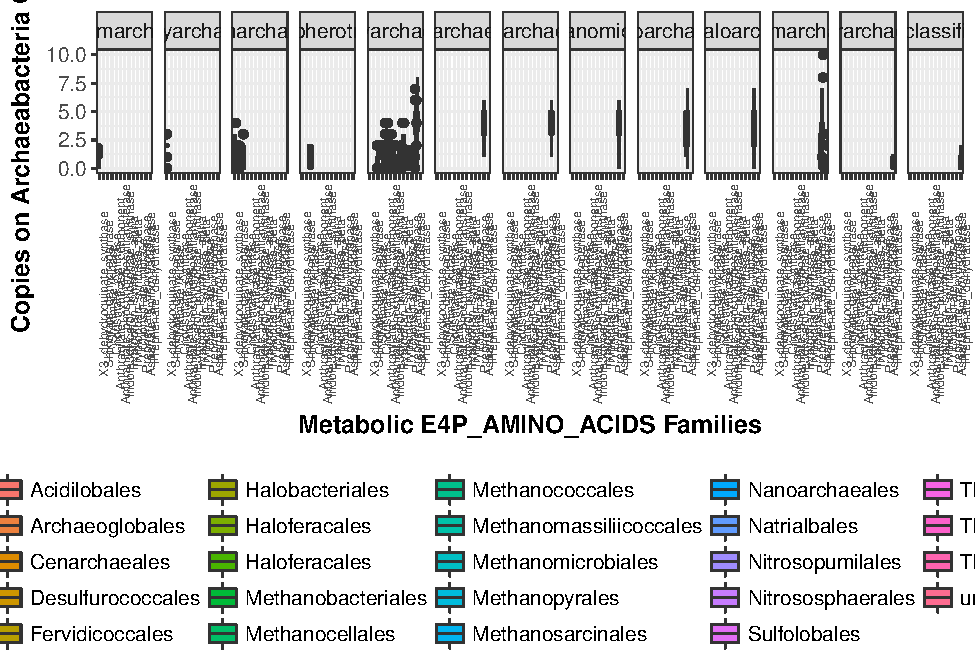
\includegraphics{tesis_files/figure-latex/ArcheaeBoxPlotByPhylum-9} \end{center}
  
  \begin{Shaded}
  \begin{Highlighting}[]
  \CommentTok{#+ geom_jitter(aes(color=MetFam_BP.m$Phylum))}
  
  
  \NormalTok{MetFam=}\KeywordTok{subset}\NormalTok{(ArchaeasCentral,Pathway==}\StringTok{"PYR_THR_AA"}\NormalTok{)}
  \NormalTok{MetFam_BP.m=ArchaeasHeatPlotBP.m[ArchaeasHeatPlotBP.m$variable %in%}\StringTok{ }\NormalTok{MetFam$Enzyme,]}
  \KeywordTok{ggplot}\NormalTok{(MetFam_BP.m, }\KeywordTok{aes}\NormalTok{(}\DataTypeTok{x=}\NormalTok{MetFam_BP.m$variable, }\DataTypeTok{y=}\NormalTok{MetFam_BP.m$value, }\DataTypeTok{fill=}\NormalTok{Order))+}\StringTok{ }\KeywordTok{labs}\NormalTok{(}\DataTypeTok{x =} \StringTok{"Metabolic Families on PYR_THR_AA pathway "}\NormalTok{, }\DataTypeTok{y =} \StringTok{"Copies on Archaeabacteria Genomes"}\NormalTok{,}\DataTypeTok{text =} \KeywordTok{element_text}\NormalTok{(}\DataTypeTok{size=}\DecValTok{12}\NormalTok{)) +}\StringTok{ }\KeywordTok{geom_boxplot}\NormalTok{() +}\StringTok{ }\KeywordTok{facet_grid}\NormalTok{(. ~}\StringTok{ }\NormalTok{Phylum)+}\KeywordTok{theme_bw}\NormalTok{() +}\KeywordTok{theme}\NormalTok{(}\DataTypeTok{plot.title =} \KeywordTok{element_text}\NormalTok{(}\DataTypeTok{size =} \DecValTok{14}\NormalTok{, }\DataTypeTok{face =} \StringTok{"bold"}\NormalTok{), }\DataTypeTok{text =} \KeywordTok{element_text}\NormalTok{(}\DataTypeTok{size =} \DecValTok{12}\NormalTok{), }\DataTypeTok{axis.title =} \KeywordTok{element_text}\NormalTok{(}\DataTypeTok{face=}\StringTok{"bold"}\NormalTok{), }\DataTypeTok{axis.text.x=}\KeywordTok{element_text}\NormalTok{(}\DataTypeTok{angle =} \DecValTok{90}\NormalTok{,}\DataTypeTok{size =} \DecValTok{6}\NormalTok{), }\DataTypeTok{legend.position =} \StringTok{"bottom"}\NormalTok{)}
  \end{Highlighting}
  \end{Shaded}
  
  \begin{center}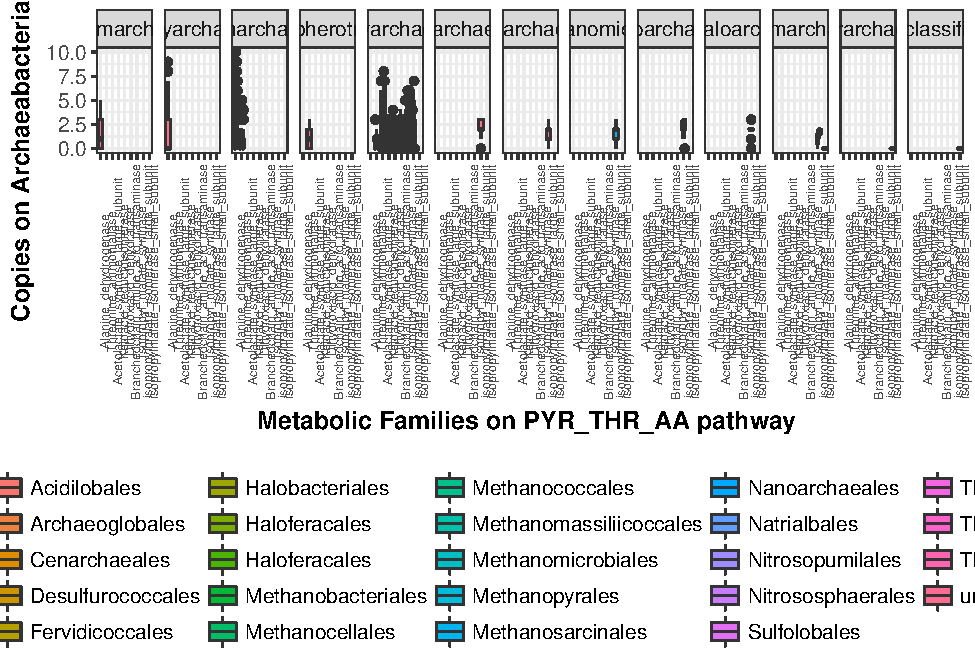
\includegraphics{tesis_files/figure-latex/ArcheaeBoxPlotByPhylum-10} \end{center}
  
  \begin{Shaded}
  \begin{Highlighting}[]
  \CommentTok{#+ geom_jitter(aes(color=MetFam_BP.m$Phylum))}
  
  \CommentTok{#ggsave("chapter3/expansion_plotArchaeas.pdf", plot = expansion_plotArchaea,height = 8, width = 7)}
  \end{Highlighting}
  \end{Shaded}
  
  \clearpage 
  
  \section{Central pathway expansions}\label{central-pathway-expansions}
  
  Heat plot of central pathways expansions, Needs to be phylogenetically
  sorted.
  
  \begin{figure}[h!tbp]
  \centering
  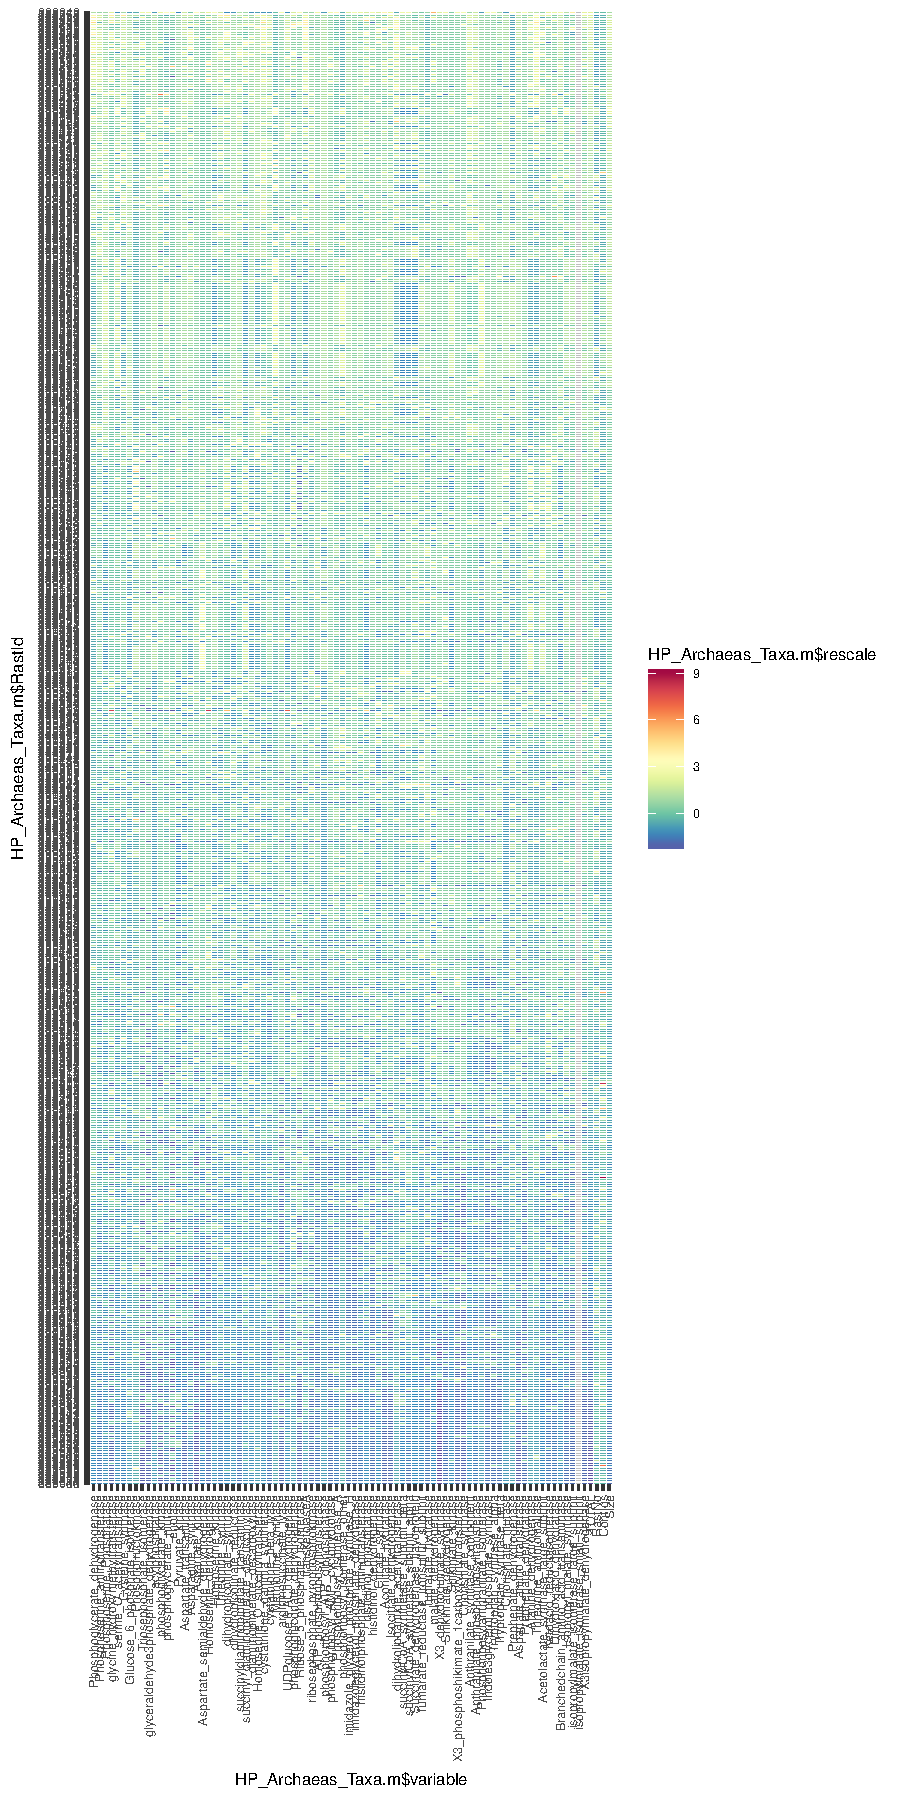
\includegraphics[angle = 0,scale = 0.6]{chapter3/ArchaeasHeatPlot.pdf}
  \caption[Archaeas Heatplot]{\normalsize{Archaeas Heatplot}}
  \label{fig:ArchaeaPlot}
  \end{figure}
  
  Here is a reference to the HeatPlot: \autoref{fig:ArchaeaPlot}.
  \clearpage 
  
  \section{Genome Size correlations}\label{genome-size-correlations}
  
  \subsection{Correlation between genome size and AntiSMASH
  products}\label{correlation-between-genome-size-and-antismash-products}
  
  Genome size vs Total antismash cluster coloured by order
  
  \begin{figure}[h!tbp]
  \centering
  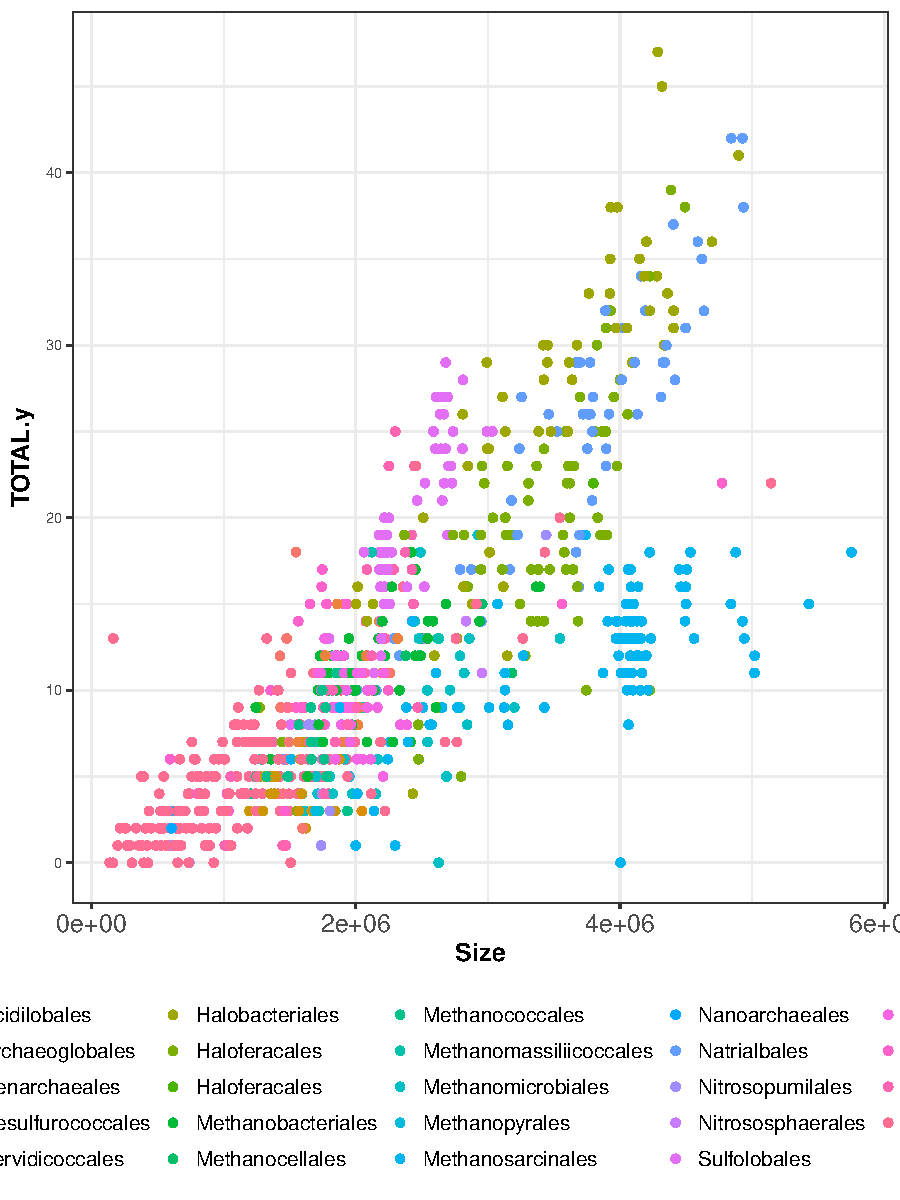
\includegraphics[angle = 0,scale = 0.6]{chapter3/ArchaeasSMASHvsSizebyOrder.pdf}
  \caption[Correlation between Archaeas genome size and antismash Natural products detection colored by Order]{\normalsize{Correlation between Archaeas genome size and antismash Natural products detection colored by Order}}
  \label{fig:ArchaeasSMASHvsSizebyOrder}
  \end{figure}
  
  Here is a reference to Genome size vs Total antismash cluster:
  \autoref{fig:ArchaeasSMASHvsSizebyOrder}. \clearpage
  
  Genome size vs Total antismash cluster detected splitted by order
  
  \begin{figure}[h!tbp]
  \centering
  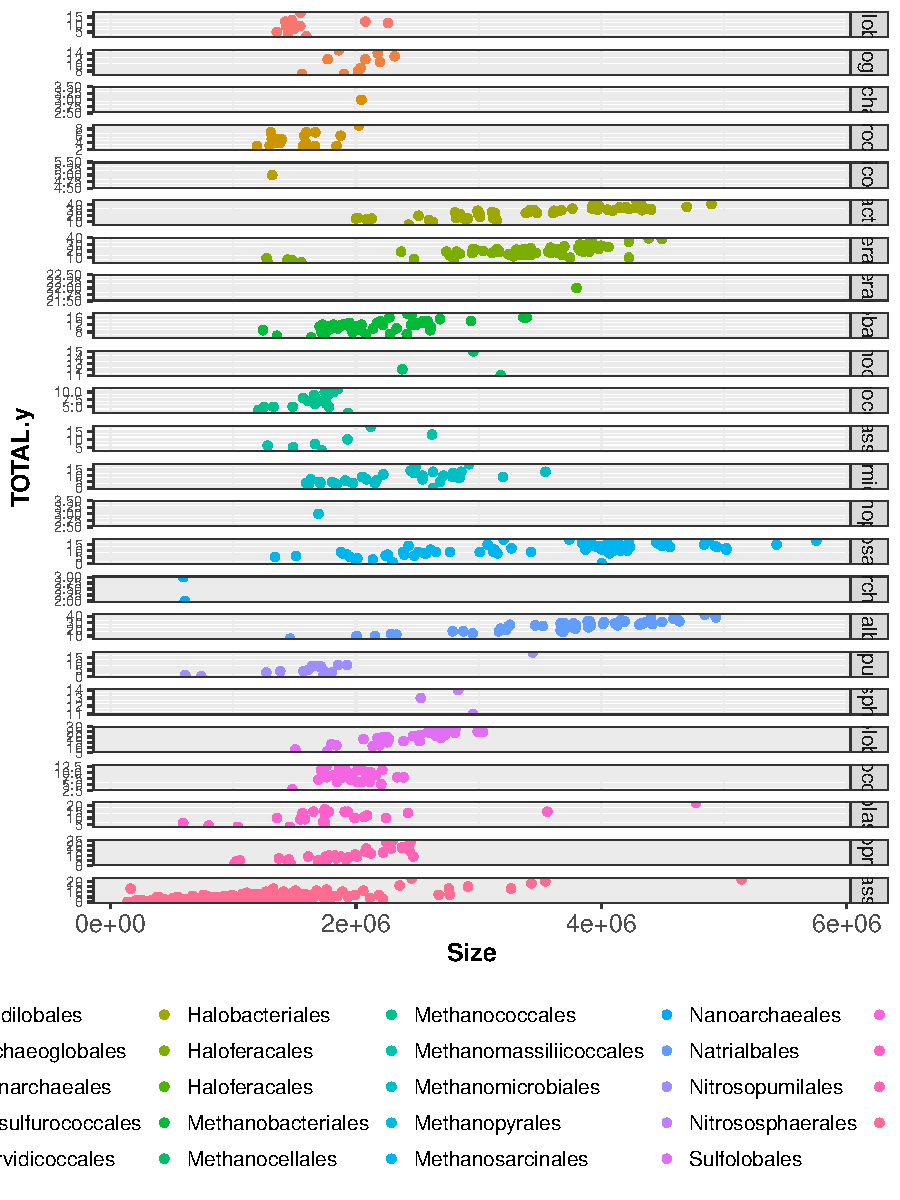
\includegraphics[angle = 0,scale = 0.6]{chapter3/ArchaeasSMASHvsSizeGridOrder.pdf}
  \caption[Correlation between Archaeas genome size and antismash Natural products detection grided by Order]{\normalsize{Correlation between Archaeas genome size and antismash Natural products detection grided by Order}}
  \label{fig:ArchaeasSMASHvsSizeGridOrder}
  \end{figure}
  
  Here is a reference to Correlation between genome size and antismash
  Natural products detection grided by Order plot:
  \autoref{fig:ArchaeasSMASHvsSizeGridOrder}. \clearpage 
  
  \subsection{Correlation between genome size and Central pathway
  expansions}\label{correlation-between-genome-size-and-central-pathway-expansions}
  
  Genome size vs Total central pathway expansion coloured by order
  
  \begin{figure}[h!tbp]
  \centering
  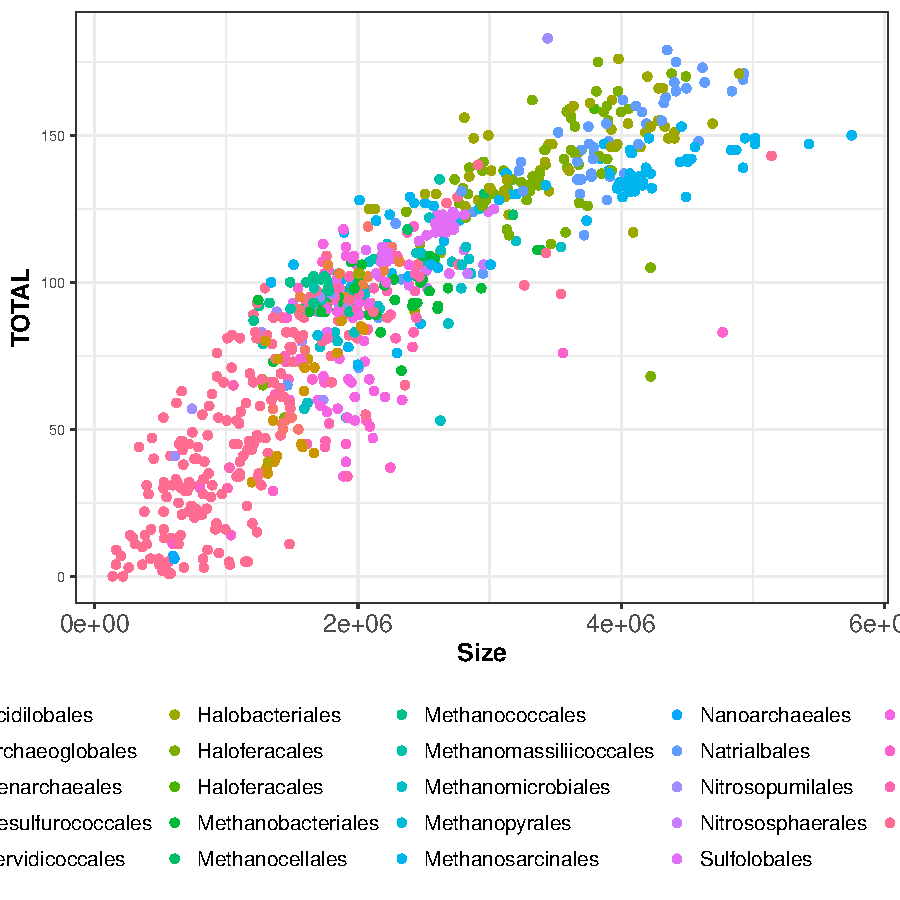
\includegraphics[angle = 0,scale = 1]{chapter3/ArchaeasSizevsExpansionsbyOrder.pdf}
  \caption[Correlation between Archaeas genome size and central pathway expansions ]{\normalsize{Correlation between Archaeas genome size and central pathway expansions }}
  \label{fig:ArchaeasSizevsExpansionsbyOrder}
  \end{figure}
  
  Here is a reference to the size vs Total central pathway expansion plot:
  \autoref{fig:ArchaeasSizevsExpansionsbyOrder}. \clearpage 
  
  Genome size vs Total central pathway expansion grided by order
  
  \begin{figure}[h!tbp]
  \centering
  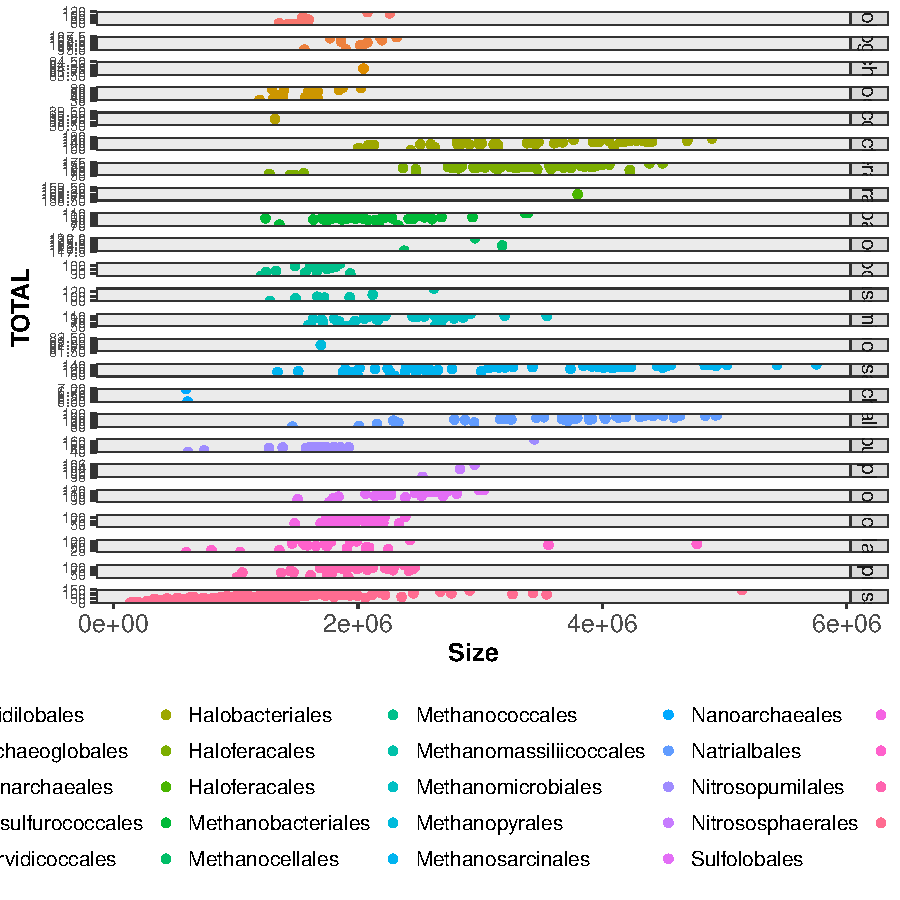
\includegraphics[angle = 0,scale = 1]{chapter3/ArchaeasSizevsExpansionsGridbyOrder.pdf}
  \caption[Correlation between Archaeas genome size and central pathway expansions grided by order]{\normalsize{Correlation between Archaeas genome size and central pathway expansions grided by order}}
  \label{fig:ArchaeasSizevsExpansionsGridbyOrder}
  \end{figure}
  
  Here is a reference to the Genome size vs Total central pathway
  expansion grided by order plot:
  \autoref{fig:ArchaeasSizevsExpansionsGridbyOrder}. \clearpage 
  
  Correlation between genome size and each of the central pathway
  families. Data are coloured by metabolic family instead of coloured by
  taxonomical order. This treatment allows to answer how differente
  metabolic families grows when genome size grow.\\
  Also I want to add form given by taxonomical order.
  
  \begin{verbatim}
  Warning: The shape palette can deal with a maximum of 6 discrete values
  because more than 6 becomes difficult to discriminate; you have
  24. Consider specifying shapes manually if you must have them.
  \end{verbatim}
  
  \begin{verbatim}
  Warning: Removed 64823 rows containing missing values (geom_point).
  \end{verbatim}
  
  Genome size vs Total central pathway expansion coloured by metabolic
  Family
  
  \begin{figure}[h!tbp]
  \centering
  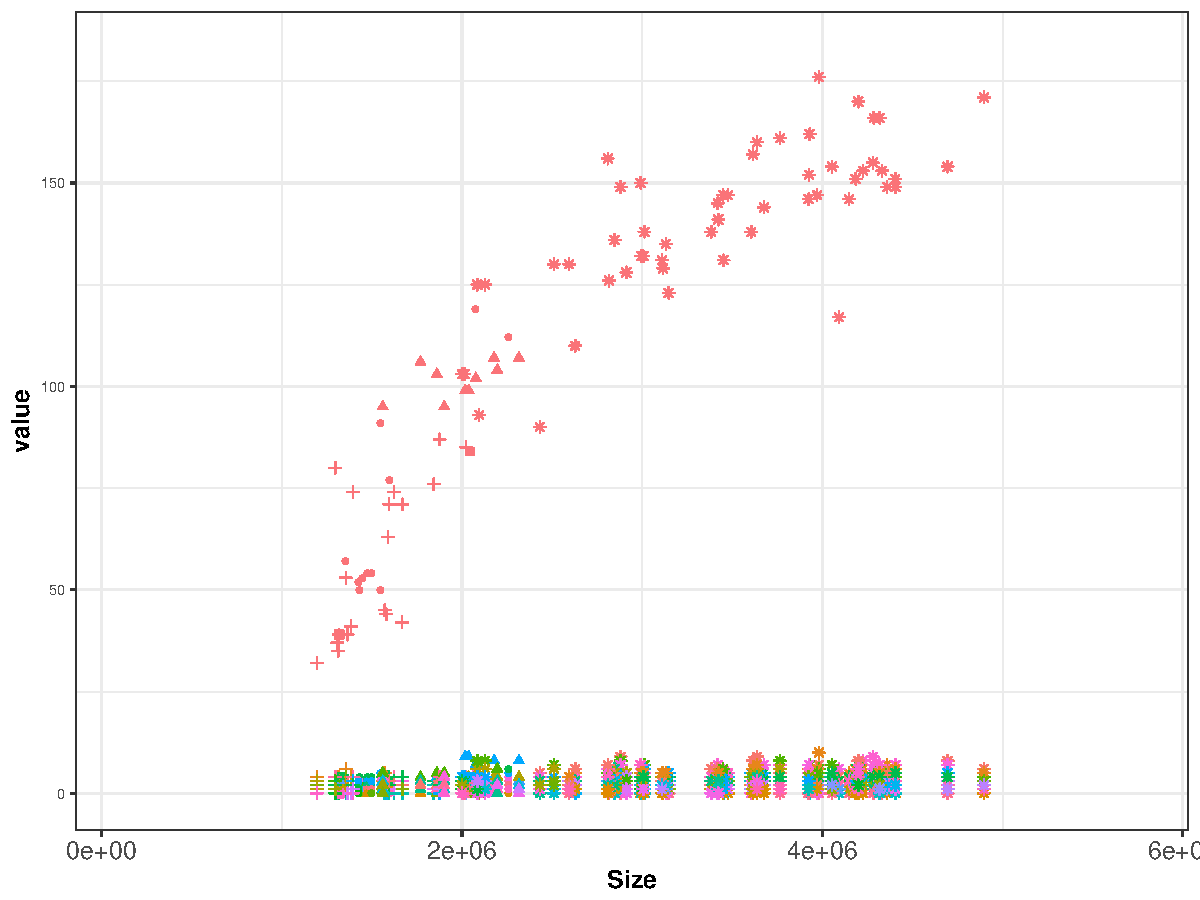
\includegraphics[angle = 0,scale = 0.6]{chapter3/ArchaeasSizevsExpansionsbyMetabolicFamily.pdf}
  \caption[Correlation between Archaeas Genome size vs Total central pathway expansion coloured by metabolic Family]{\normalsize{Correlation between Archaeas Genome size vs Total central pathway expansion coloured by metabolic Family}}
  \label{fig:ArchaeasSizevsExpansionsbyMetabolicFamily}
  \end{figure}
  
  Here is a reference to the Genome size vs Total central pathway
  expansion coloured by metabolic Family plot:
  \autoref{fig:ArchaeasSizevsExpansionsbyMetabolicFamily}. \clearpage 
  
  Future Work: Genome size vs Total central pathway expansion grided by
  metabolic Family For clarity I need to also grid and group by Metabolic
  Pathway
  
  Here is a reference to Genome size vs Total central pathway expansion
  grided by metabolic Family plot:
  \autoref{fig:ArchaeasExpansionsbyMetabolicFamilyGrid}. \clearpage 
  
  \section{Natural products}\label{natural-products}
  
  \subsection{Natural products recruitments from EvoMining
  heatplot}\label{natural-products-recruitments-from-evomining-heatplot}
  
  We can see natural products recruitment after central pathways
  expansions colored by their kingdom.\\
  Natural products recruited by metabolic family, colored by phylogenetic
  origin.
  
  Recruitments after central pathways expansions coloured by Kingdom
  
  \begin{figure}[h!tbp]
  \centering
  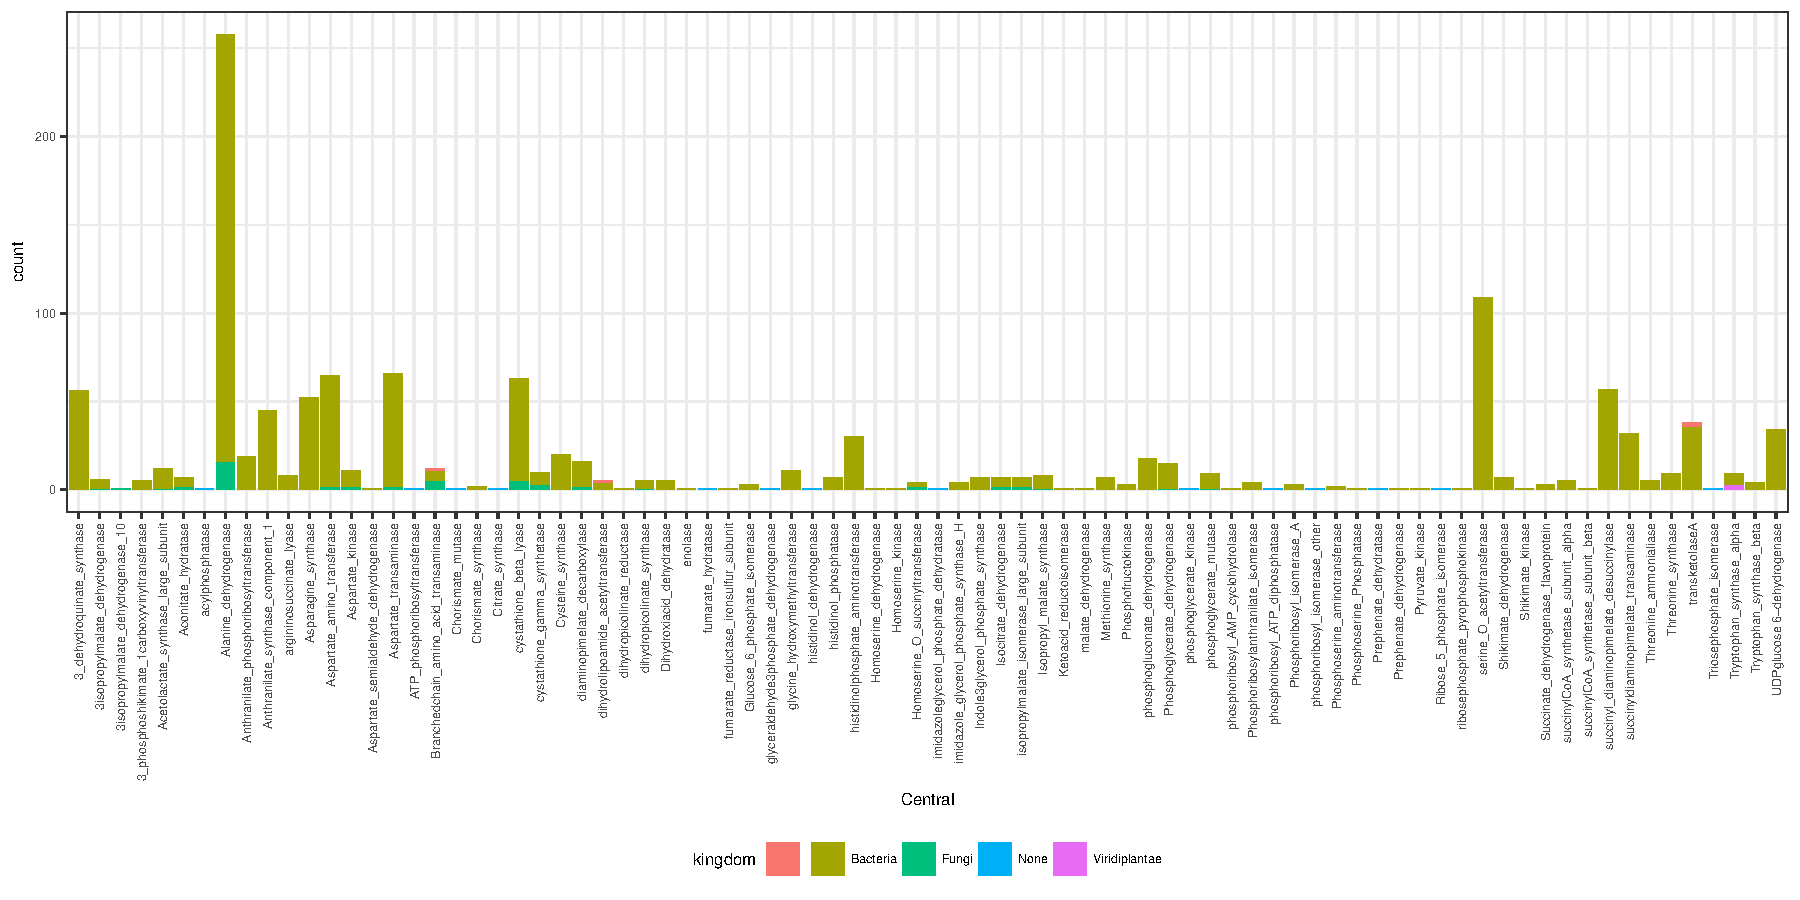
\includegraphics[angle = 0,scale = 0.6]{chapter3/ArchaeasRecruitmentsbyKingdom.pdf}
  \caption[Archaeas Recruitmens on central families coloured by kingdom]{\normalsize{Archaeas Recruitmens on central families coloured by kingdom}}
  \label{fig:ArchaeasRecruitmentsbyKingdom}
  \end{figure}
  
  Here is a reference to Recruitments after central pathways expansions
  colourd by Kingdom plot: \autoref{fig:ArchaeasRecruitmentsbyKingdom}.
  
  \clearpage 
  Recruitments after central pathways expansions colourd by taxonomy
  
  \begin{figure}[h!tbp]
  \centering
  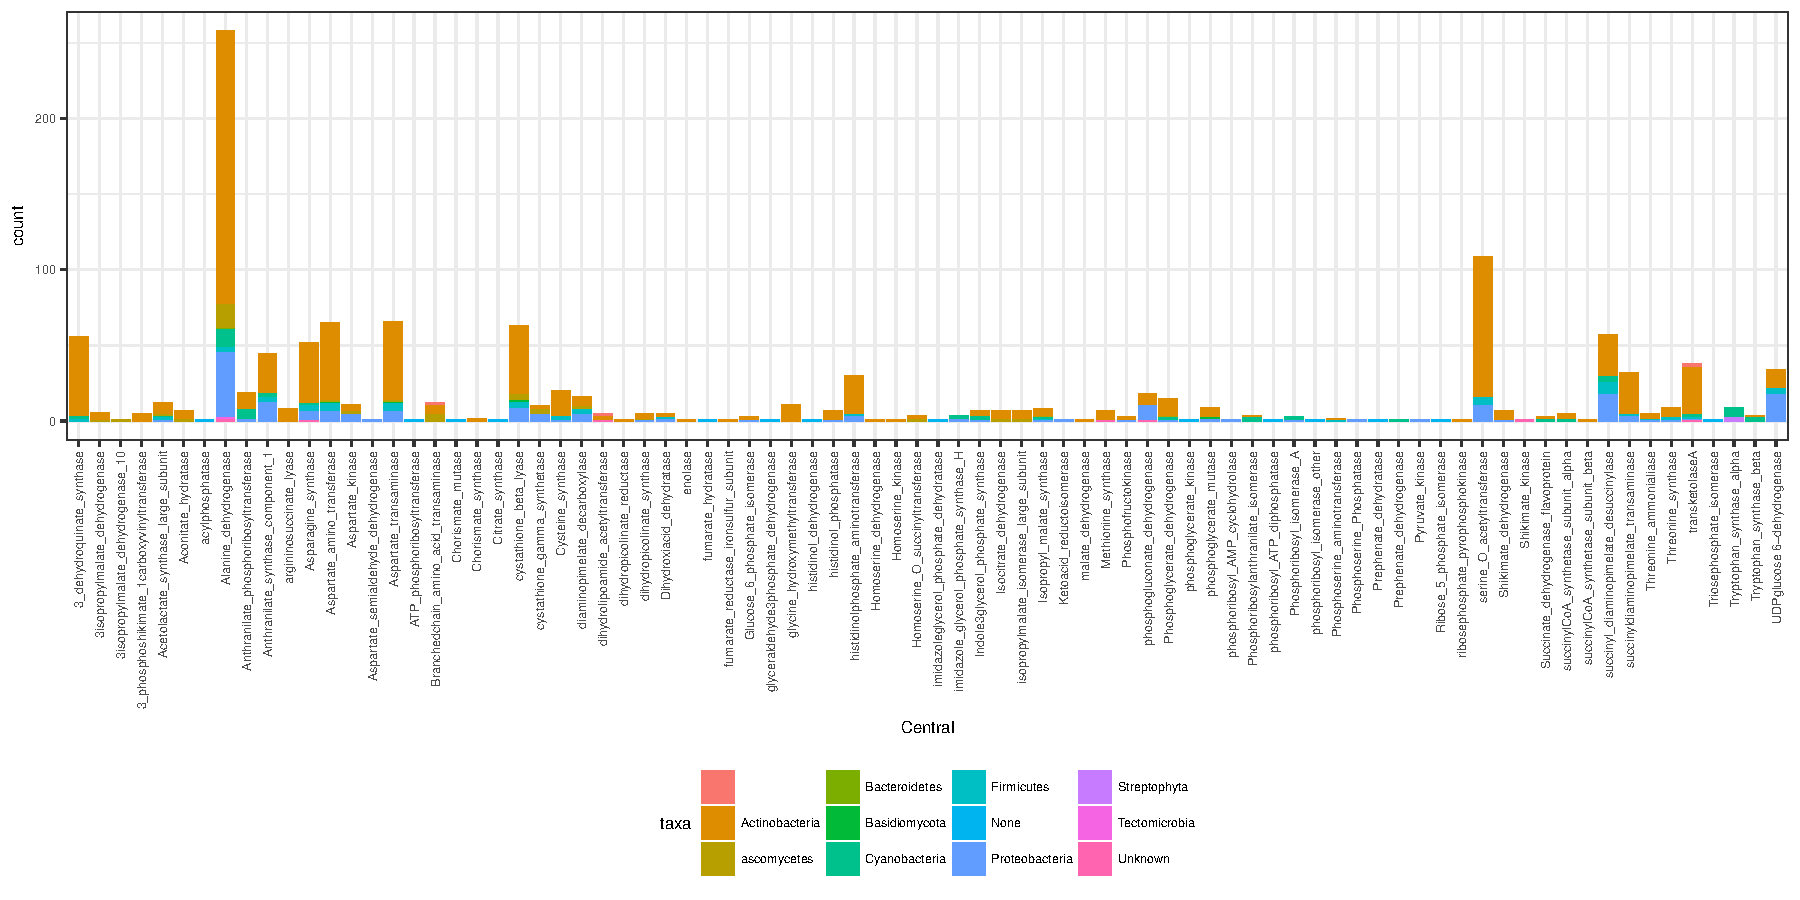
\includegraphics[angle = 0,scale = 0.5]{chapter3/ArchaeasRecruitmentsbyTaxa.pdf}
  \caption[Archaeas Recruitmens on central families coloured by taxonomy]{\normalsize{Archaeas Recruitmens on central families coloured by taxonomy}}
  \label{fig:ArchaeasRecruitmentsbyTaxa}
  \end{figure}
  
  Here is a reference to Recruitments after central pathways expansions
  colourd by taxa plot: \autoref{fig:ArchaeasRecruitmentsbyTaxa}.
  \clearpage 
  
  \section{Archaeas AntiSMASH}\label{archaeas-antismash}
  
  Taxonomical diversity on Archaeasbacteria Data
  
  \begin{figure}[h!tbp]
  \centering
  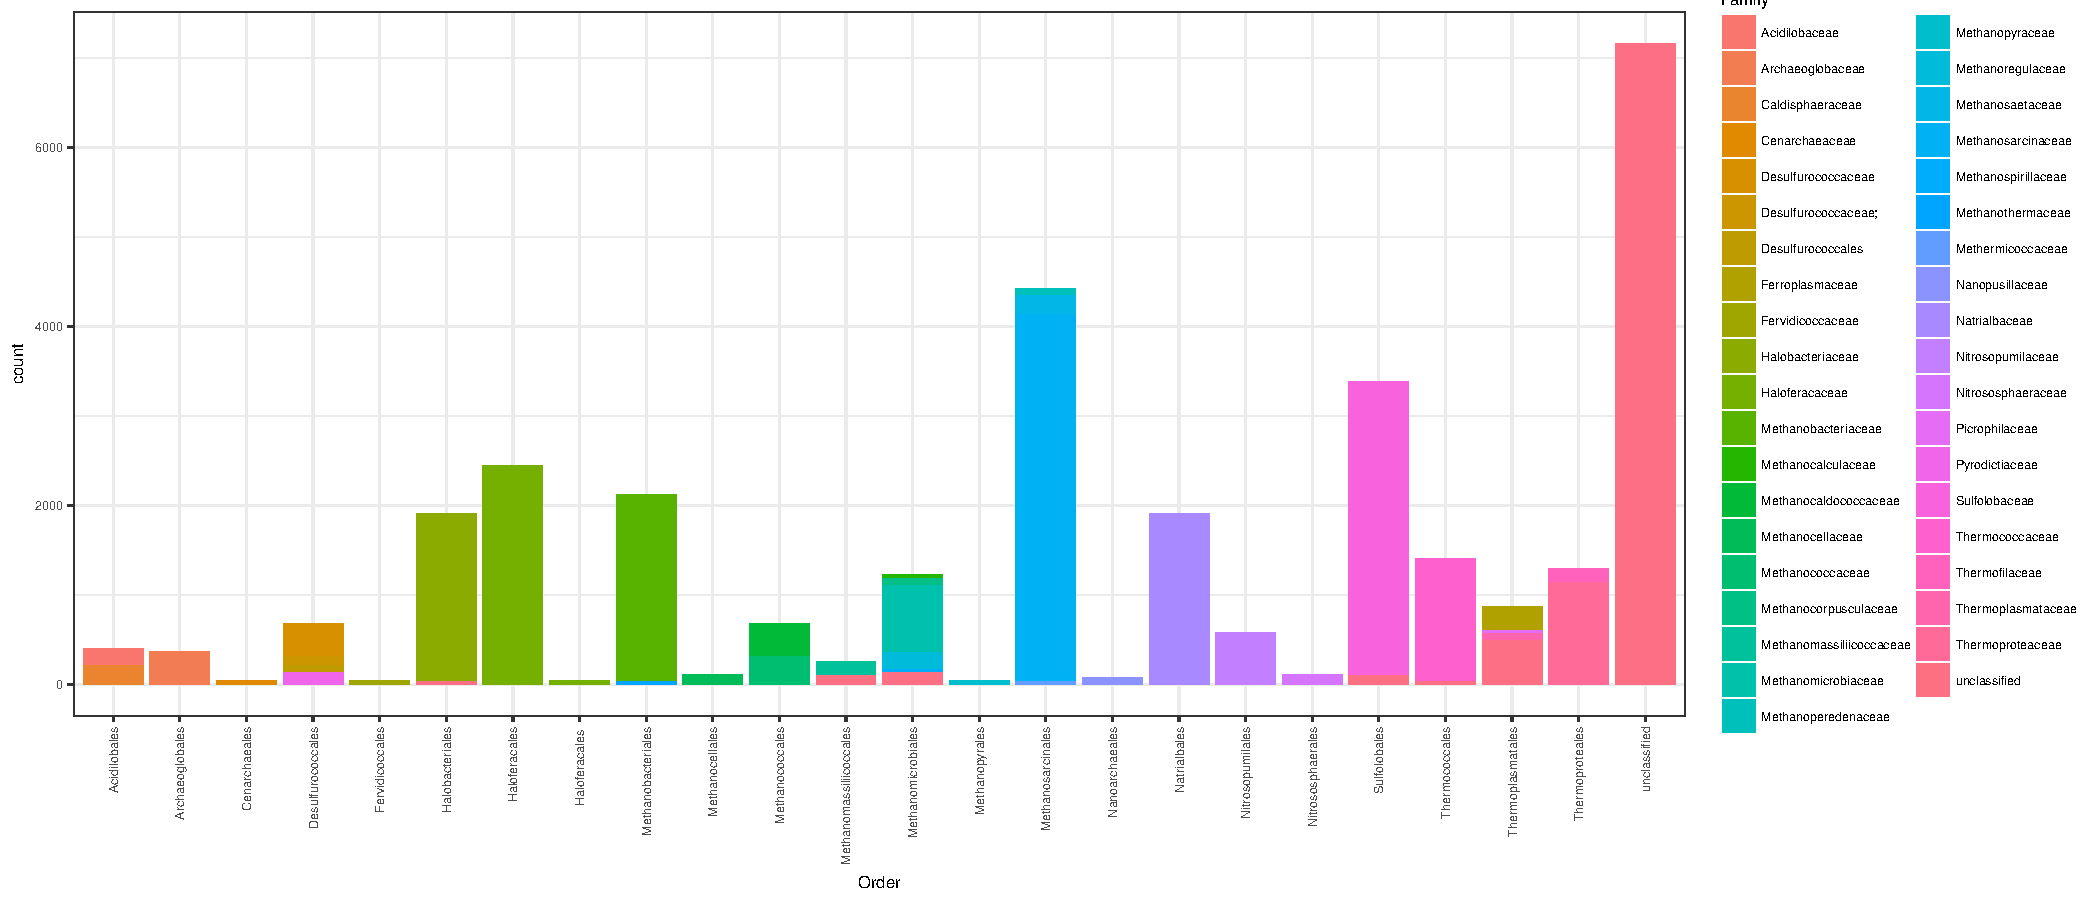
\includegraphics[angle = 0,scale = 0.6]{chapter3/ArchaeasDiversity.pdf}
  \caption[Archaeas Diversity]{\normalsize{Archaeas Diversity}}
  \label{fig:ArchaeasDiversity}
  \end{figure}
  
  Here is a reference to Recruitments after central pathways expansions
  colourd by taxa plot: \autoref{fig:ArchaeasDiversity}. \clearpage
  
  Smash diversity
  
  \begin{figure}[h!tbp]
  \centering
  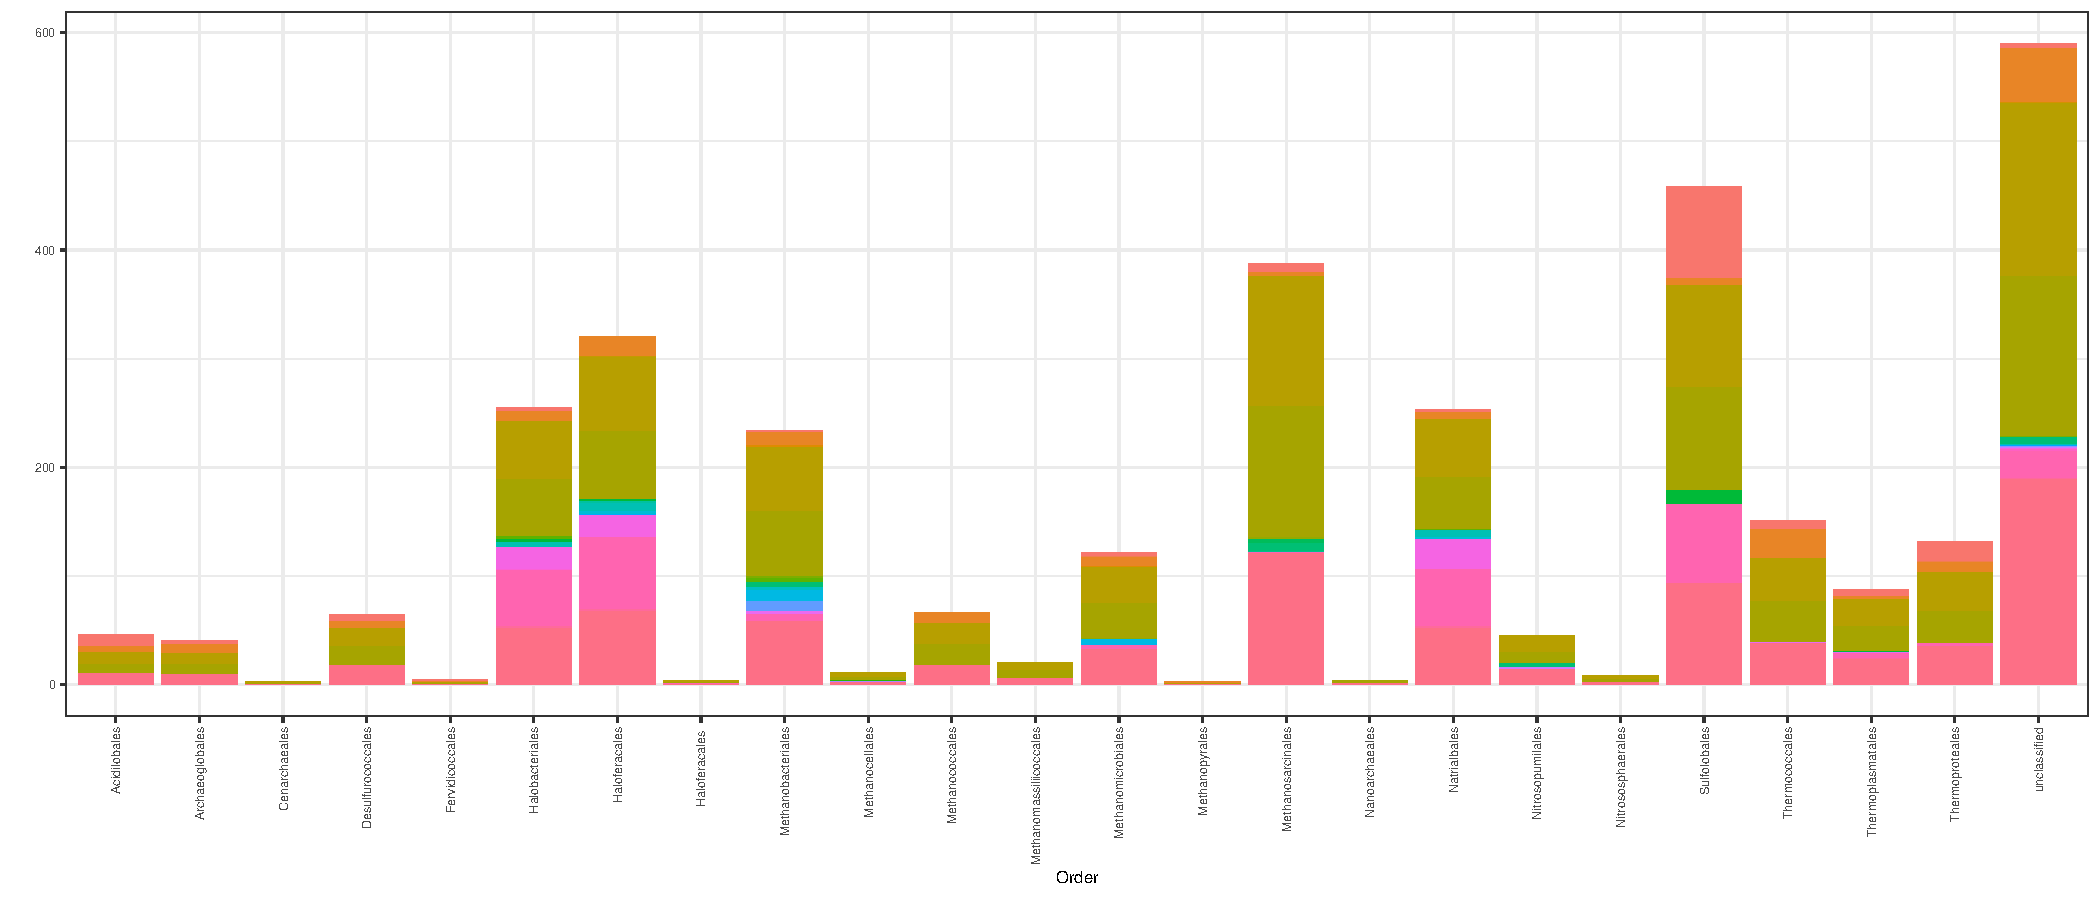
\includegraphics[angle = 0,scale = 0.5]{chapter3/ArchaeasSmash.pdf}
  \caption[Archaeas Smash Taxonomical Diversity]{\normalsize{Archaeas Smash Taxonomical Diversity}}
  \label{fig:ArchaeasSmash}
  \end{figure}
  
  Here is a reference to Recruitments after central pathways expansions
  colourd by taxa plot: \autoref{fig:ArchaeasSmash}. \clearpage
  
  \subsection{AntisSMASH vs Central
  Expansions}\label{antissmash-vs-central-expansions}
  
  Is it a correlation between pangenome grow and central pathways
  expansions?
  
  Total central pathway expansions by genome vs Total antismash cluster
  detected coloured by order
  
  \begin{figure}[h!tbp]
  \centering
  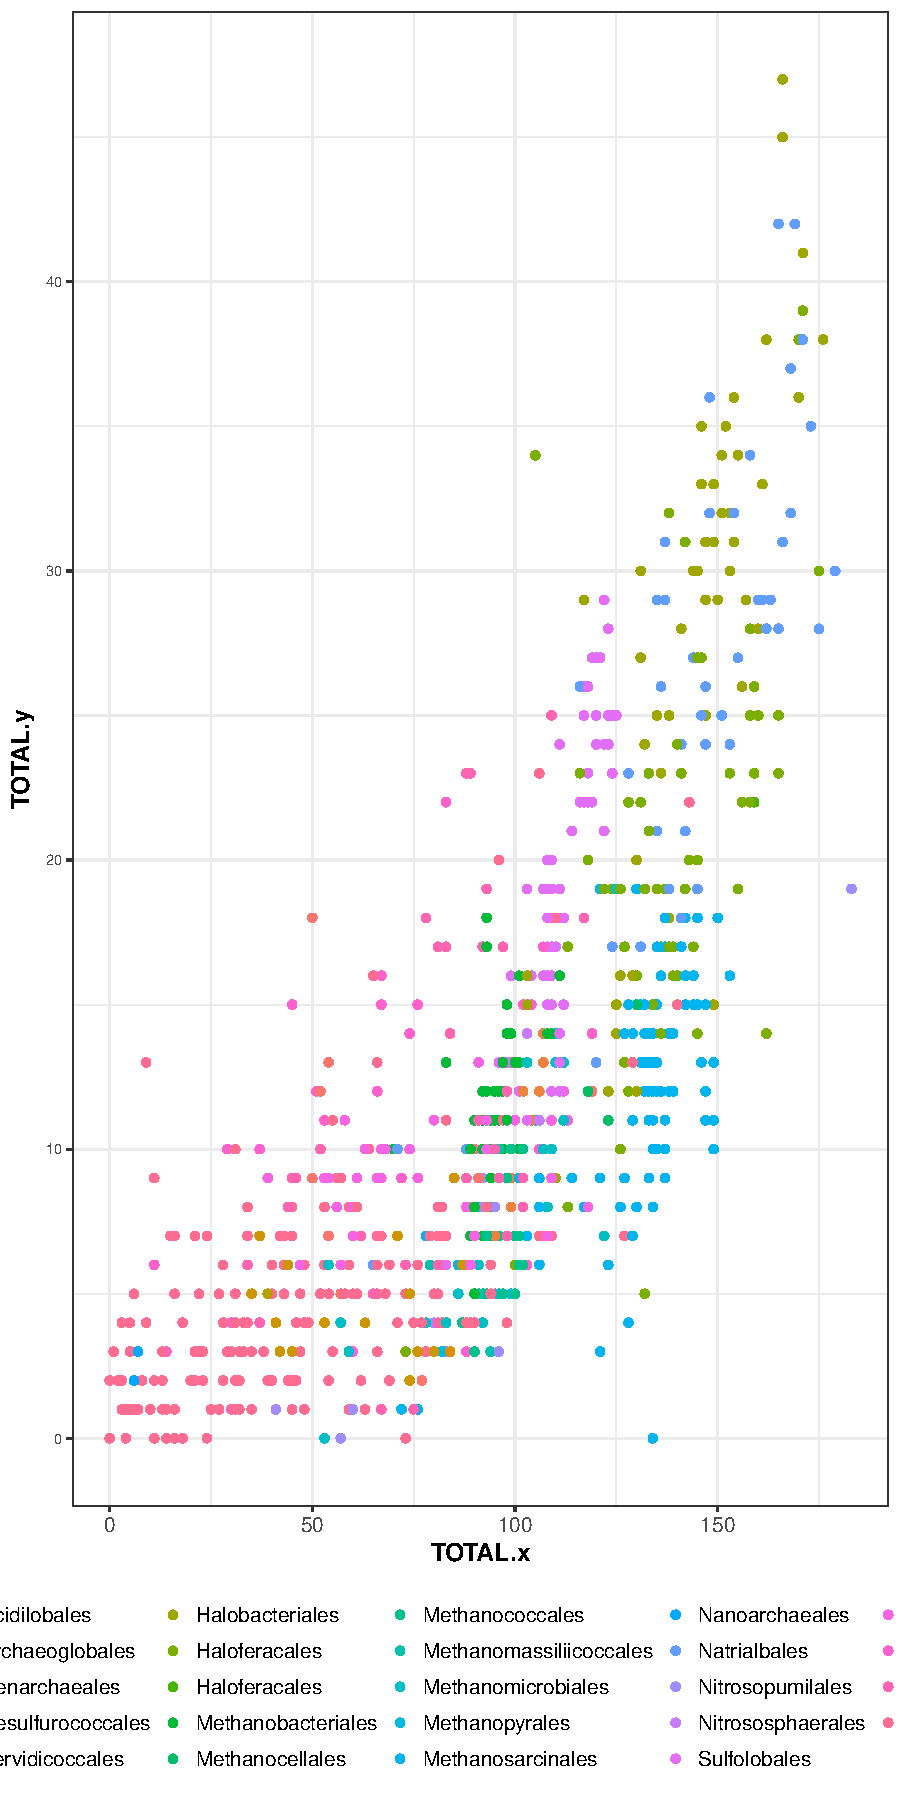
\includegraphics[angle = 0,scale = 0.5]{chapter3/ArchaeasSMASHvsExpansionsbyOrder.pdf}
  \caption[Correlation between Archaeas central pathway expansions and antismash Natural products detection]{\normalsize{Correlation between Archaeas central pathway expansions and antismash Natural products detection}}
  \label{fig:ArchaeasSMASHvsExpansionsbyOrder}
  \end{figure}
  
  Here is a reference to the expansions vs antismash NP's clusters plot:
  \autoref{fig:ArchaeasSMASHvsExpansionsbyOrder}. \clearpage 
  
  Total central pathway expansions by genome vs Total antismash cluster
  detected splitted by order
  
  \begin{figure}[h!tbp]
  \centering
  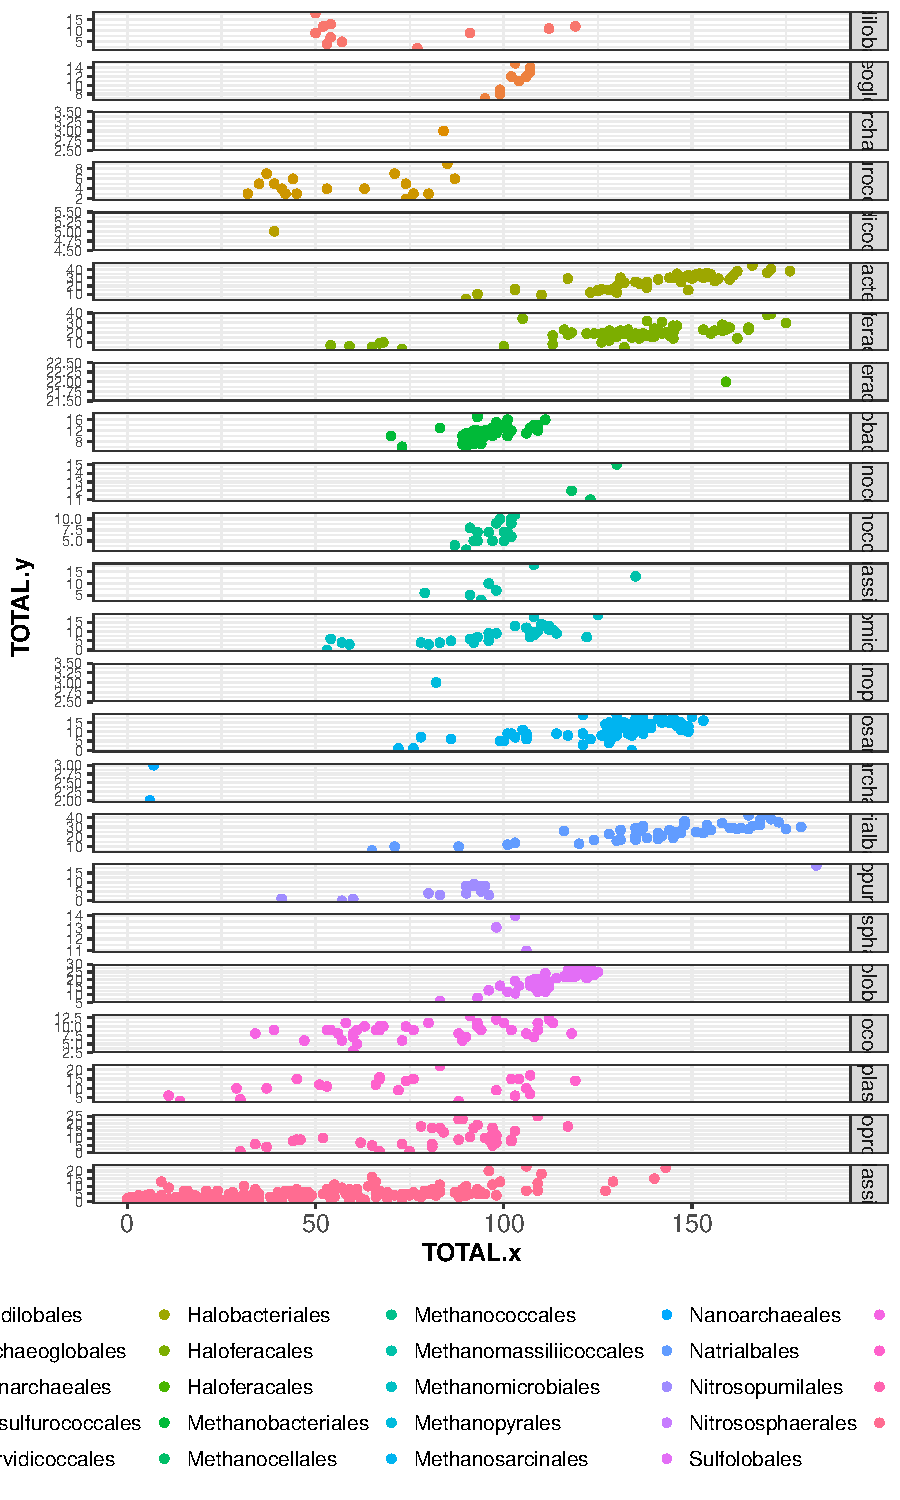
\includegraphics[angle = 0,scale = 0.5]{chapter3/ArchaeasSMASHvsExpansionsbyOrderGRID.pdf}
  \caption[Correlation between Archaeas central pathway expnasions and antismash Natural products detection]{\normalsize{Correlation between Archaeas central pathway expnasions and antismash Natural products detection}}
  \label{fig:ArchaeasSMASHvsExpansionsbyOrderGRID}
  \end{figure}
  
  Here is a reference to the expansions vs antismash NP's clusters
  splitted by order plot
  \autoref{fig:ArchaeasSMASHvsExpansionsbyOrderGRID}. \clearpage 
  
  AntisMAsh vs Expansions by taxonomic Family
  
  Natural products colured by family
  
  \begin{figure}[h!tbp]
  \centering
  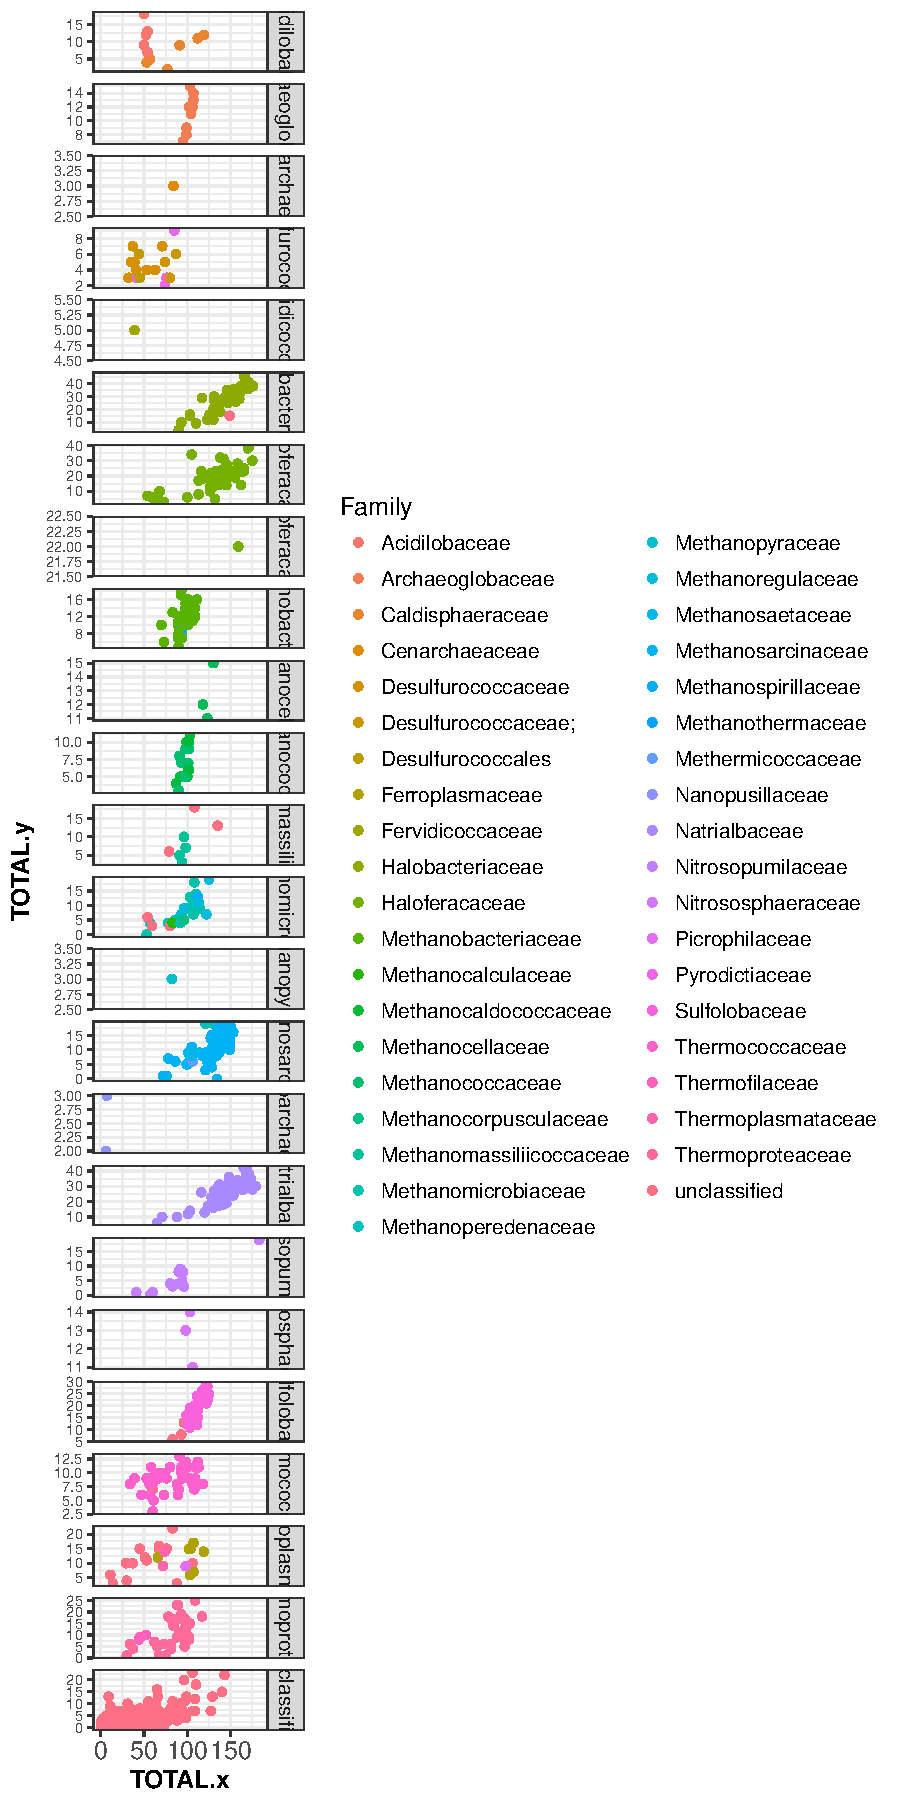
\includegraphics[angle = 0,scale = 0.6]{chapter3/Archaeasnpf.pdf}
  \caption[Archaeas Natural products by family]{\normalsize{Archaeas Natural products by family}}
  \label{fig:Archaeasnpf}
  \end{figure}
  
  Here is a reference to the Natural products colured by family plot
  \autoref{fig:Archaeasnpf}. \clearpage 
  
  \section{Selected trees from
  EvoMining}\label{selected-trees-from-evomining}
  
  Phosphoribosyl\_isomerase\_3 family\\
  Figure from EvoMining
  
  \begin{figure}[h!tbp]
  \centering
  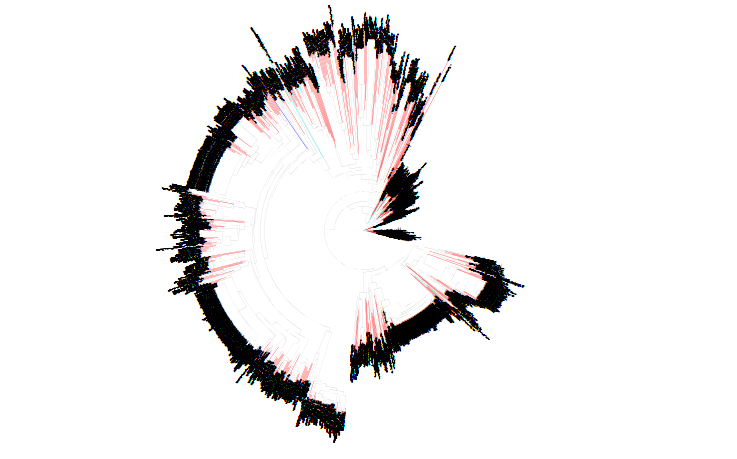
\includegraphics[angle = 180,scale = 0.25]{chapter3/tree41.png}
  \caption[Phosphoribosyl isomerase A EvoMiningtree]{\normalsize{Phosphoribosyl isomerase A EvoMiningtree}}
  \label{fig:Phosphoribosyl_isomerase_A_evo_tree}
  \end{figure}\begin{figure}[h!tbp]
  \centering
  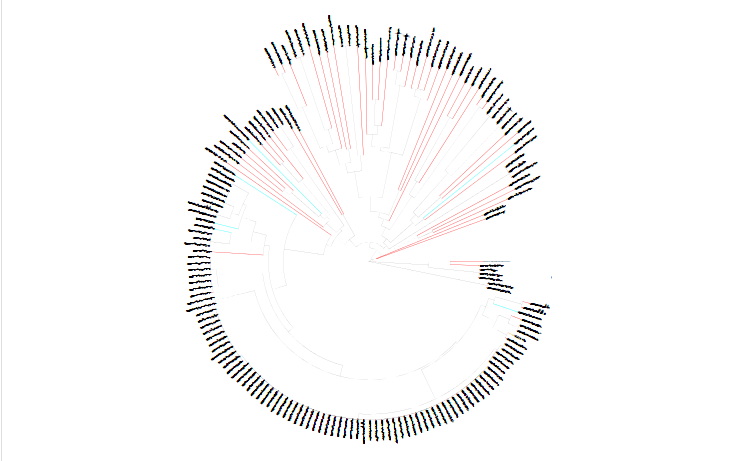
\includegraphics[angle = 180,scale = 0.25]{chapter3/tree42.png}
  \caption[Phosphoribosyl isomerase other EvoMiningtree]{\normalsize{Phosphoribosyl isomerase other EvoMiningtree}}
  \label{fig:Phosphoribosyl_isomerase_other_evo_tree}
  \end{figure}\begin{figure}[h!tbp]
  \centering
  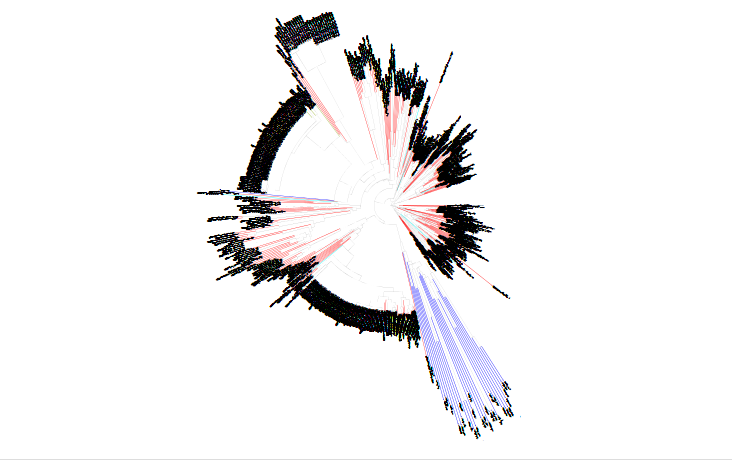
\includegraphics[angle = 180,scale = 0.25]{chapter3/tree65.png}
  \caption[Phosphoribosyl anthranilate isomerase EvoMiningtree]{\normalsize{Phosphoribosyl anthranilate isomerase EvoMiningtree}}
  \label{fig:Phosphoribosylanthranilate_isomerase_evo_tree}
  \end{figure}
  
  \clearpage 
  
  \hypertarget{section}{\section{}\label{section}}
  
  Other possible databases Archaeal signatures \emph{set of
  protein-encoding genes that function uniquely within the Archaea; most
  signature proteins have no recognizable bacterial or eukaryal homologs}
  {[}\protect\hyperlink{ref-grahamux5farchaealux5f2000}{117}{]} \#\#
  Footnotes and Endnotes
  
  You might want to footnote something.\footnote{footnote text} The
  footnote will be in a smaller font and placed appropriately. Endnotes
  work in much the same way. More information can be found about both on
  the CUS site or feel free to reach out to
  \href{mailto:data@reed.edu}{\nolinkurl{data@reed.edu}}.
  
  \section{Bibliographies}\label{bibliographies}
  
  Of course you will need to cite things, and you will probably accumulate
  an armful of sources. There are a variety of tools available for
  creating a bibliography database (stored with the .bib extension). In
  addition to BibTeX suggested below, you may want to consider using the
  free and easy-to-use tool called Zotero. The Reed librarians have
  created Zotero documentation at
  \url{http://libguides.reed.edu/citation/zotero}. In addition, a tutorial
  is available from Middlebury College at
  \url{http://sites.middlebury.edu/zoteromiddlebury/}.
  
  \emph{R Markdown} uses \emph{pandoc} (\url{http://pandoc.org/}) to build
  its bibliographies. One nice caveat of this is that you won't have to do
  a second compile to load in references as standard \LaTeX~requires. To
  cite references in your thesis (after creating your bibliography
  database), place the reference name inside square brackets and precede
  it by the ``at'' symbol. For example, here's a reference to a book about
  worrying: {[}\protect\hyperlink{ref-Molina1994}{140}{]}. This
  \texttt{Molina1994} entry appears in a file called \texttt{thesis.bib}
  in the \texttt{bib} folder. This bibliography database file was created
  by a program called BibTeX. You can call this file something else if you
  like (look at the YAML header in the main .Rmd file) and, by default, is
  to placed in the \texttt{bib} folder.
  
  For more information about BibTeX and bibliographies, see our CUS site
  (\url{http://web.reed.edu/cis/help/latex/index.html})\footnote{{[}\protect\hyperlink{ref-reedweb2007}{141}{]}}.
  There are three pages on this topic: \emph{bibtex} (which talks about
  using BibTeX, at \url{http://web.reed.edu/cis/help/latex/bibtex.html}),
  \emph{bibtexstyles} (about how to find and use the bibliography style
  that best suits your needs, at
  \url{http://web.reed.edu/cis/help/latex/bibtexstyles.html}) and
  \emph{bibman} (which covers how to make and maintain a bibliography by
  hand, without BibTeX, at
  \url{http://web.reed.edu/cis/help/latex/bibman.html}). The last page
  will not be useful unless you have only a few sources.
  
  If you look at the YAML header at the top of the main .Rmd file you can
  see that we can specify the style of the bibliography by referencing the
  appropriate csl file. You can download a variety of different style
  files at \url{https://www.zotero.org/styles}. Make sure to download the
  file into the csl folder.
  
  \paragraph{Tips for Bibliographies}\label{tips-for-bibliographies}
  
  \begin{itemize}
  \tightlist
  \item
    Like with thesis formatting, the sooner you start compiling your
    bibliography for something as large as thesis, the better. Typing in
    source after source is mind-numbing enough; do you really want to do
    it for hours on end in late April? Think of it as procrastination.
  \item
    The cite key (a citation's label) needs to be unique from the other
    entries.
  \item
    When you have more than one author or editor, you need to separate
    each author's name by the word ``and'' e.g.
    \texttt{Author\ =\ \{Noble,\ Sam\ and\ Youngberg,\ Jessica\},}.
  \item
    Bibliographies made using BibTeX (whether manually or using a manager)
    accept \LaTeX~markup, so you can italicize and add symbols as
    necessary.
  \item
    To force capitalization in an article title or where all lowercase is
    generally used, bracket the capital letter in curly braces.
  \item
    You can add a Reed Thesis citation\footnote{{[}\protect\hyperlink{ref-noble2002}{142}{]}}
    option. The best way to do this is to use the phdthesis type of
    citation, and use the optional ``type'' field to enter ``Reed thesis''
    or ``Undergraduate thesis.''
  \end{itemize}
  
  \section{Anything else?}\label{anything-else}
  
  If you'd like to see examples of other things in this template, please
  contact the Data @ Reed team (email
  \href{mailto:data@reed.edu}{\nolinkurl{data@reed.edu}}) with your
  suggestions. We love to see people using \emph{R Markdown} for their
  theses, and are happy to help.
  
  \hypertarget{refux5flabels}{\chapter{Actinobacteria EvoMining
  Results}\label{refux5flabels}}
  
  Actinobacteria is an ancient phylum \{Referencia de luis\}
  
  \section{Tables}\label{tables-1}
  
  \begin{longtable}[c]{@{}ccl@{}}
  \caption{Correlation of Inheritance Factors for Parents and Child
  \label{tab:inher}}\tabularnewline
  \toprule
  \begin{minipage}[b]{0.29\columnwidth}\centering\strut
  Factors
  \strut\end{minipage} &
  \begin{minipage}[b]{0.47\columnwidth}\centering\strut
  Correlation between Parents \& Child
  \strut\end{minipage} &
  \begin{minipage}[b]{0.16\columnwidth}\raggedright\strut
  \strut\end{minipage}\tabularnewline
  \midrule
  \endfirsthead
  \toprule
  \begin{minipage}[b]{0.29\columnwidth}\centering\strut
  Factors
  \strut\end{minipage} &
  \begin{minipage}[b]{0.47\columnwidth}\centering\strut
  Correlation between Parents \& Child
  \strut\end{minipage} &
  \begin{minipage}[b]{0.16\columnwidth}\raggedright\strut
  \strut\end{minipage}\tabularnewline
  \midrule
  \endhead
  \begin{minipage}[t]{0.29\columnwidth}\centering\strut
  GenomeDB
  \strut\end{minipage} &
  \begin{minipage}[t]{0.47\columnwidth}\centering\strut
  1245
  \strut\end{minipage} &
  \begin{minipage}[t]{0.16\columnwidth}\raggedright\strut
  \strut\end{minipage}\tabularnewline
  \begin{minipage}[t]{0.29\columnwidth}\centering\strut
  Families
  \strut\end{minipage} &
  \begin{minipage}[t]{0.47\columnwidth}\centering\strut
  65
  \strut\end{minipage} &
  \begin{minipage}[t]{0.16\columnwidth}\raggedright\strut
  \strut\end{minipage}\tabularnewline
  \bottomrule
  \end{longtable}
  
  \clearpage
  
  \subsection{Expansions BoxPlot by metabolic
  family}\label{expansions-boxplot-by-metabolic-family-1}
  
  \begin{Shaded}
  \begin{Highlighting}[]
  \KeywordTok{label}\NormalTok{(}\DataTypeTok{path =} \StringTok{"chapter4/expansion_plotActinos.pdf"}\NormalTok{, }\DataTypeTok{caption =} \StringTok{"Expansions Boxplot"}\NormalTok{,}\DataTypeTok{label =} \StringTok{"Actino_expansion_boxplot"}\NormalTok{, }\DataTypeTok{type =} \StringTok{"figure"}\NormalTok{)}
  \end{Highlighting}
  \end{Shaded}
  
  \begin{figure}[h!tbp]
  \centering
  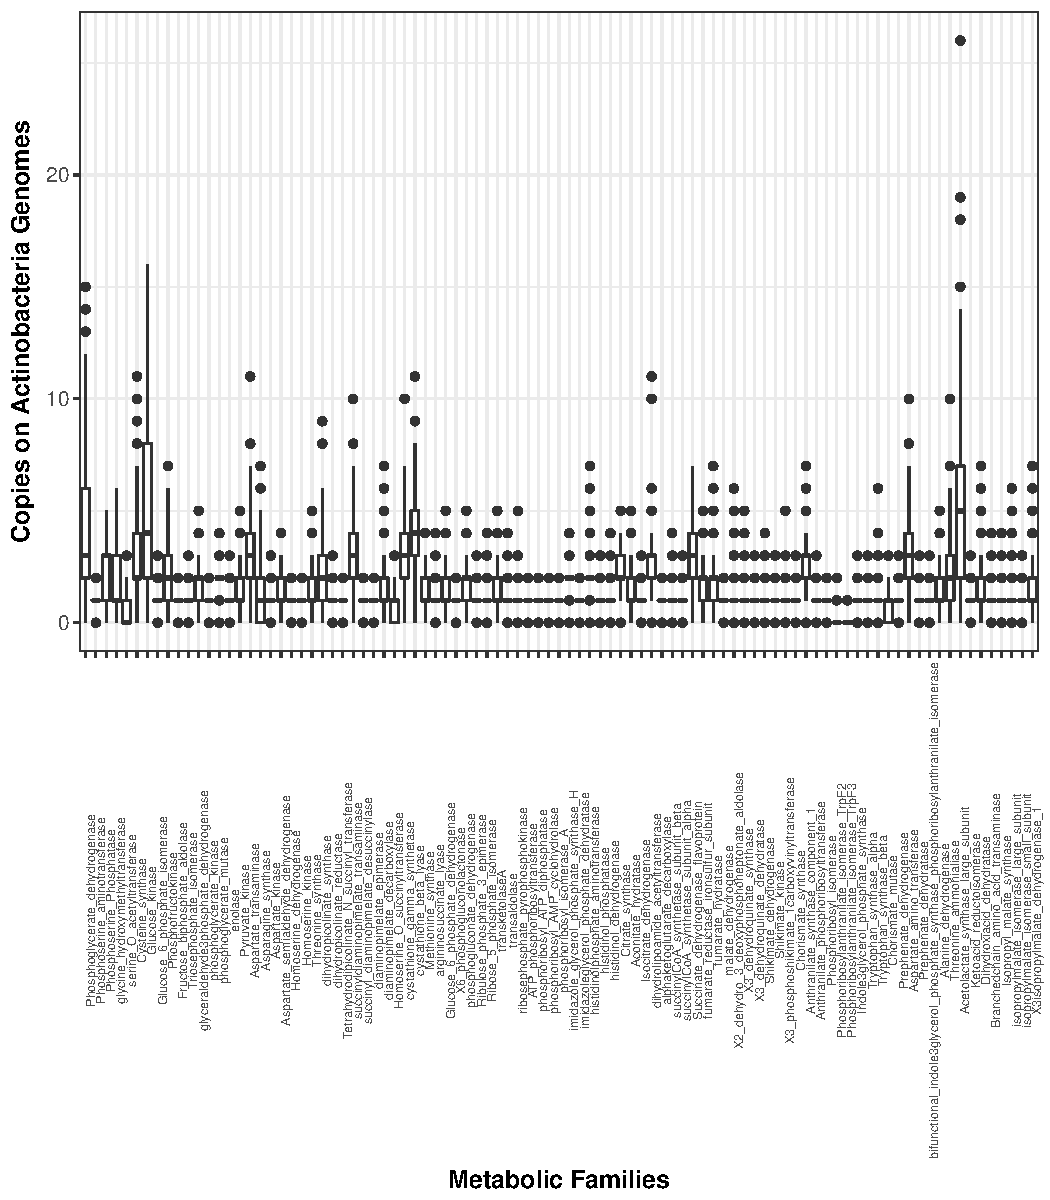
\includegraphics[angle = 0,scale = 1]{chapter4/expansion_plotActinos.pdf}
  \caption[Expansions Boxplot]{\normalsize{Expansions Boxplot}}
  \label{fig:Actino_expansion_boxplot}
  \end{figure}
  
  Here is a reference to the expansion boxplot:
  \autoref{fig:Actino_expansion_boxplot}.\\
  \clearpage 
  
  \section{Central pathway expansions}\label{central-pathway-expansions-1}
  
  Heat plot of central pathways expansions, Needs to be phylogenetically
  sorted.
  
  \begin{figure}[h!tbp]
  \centering
  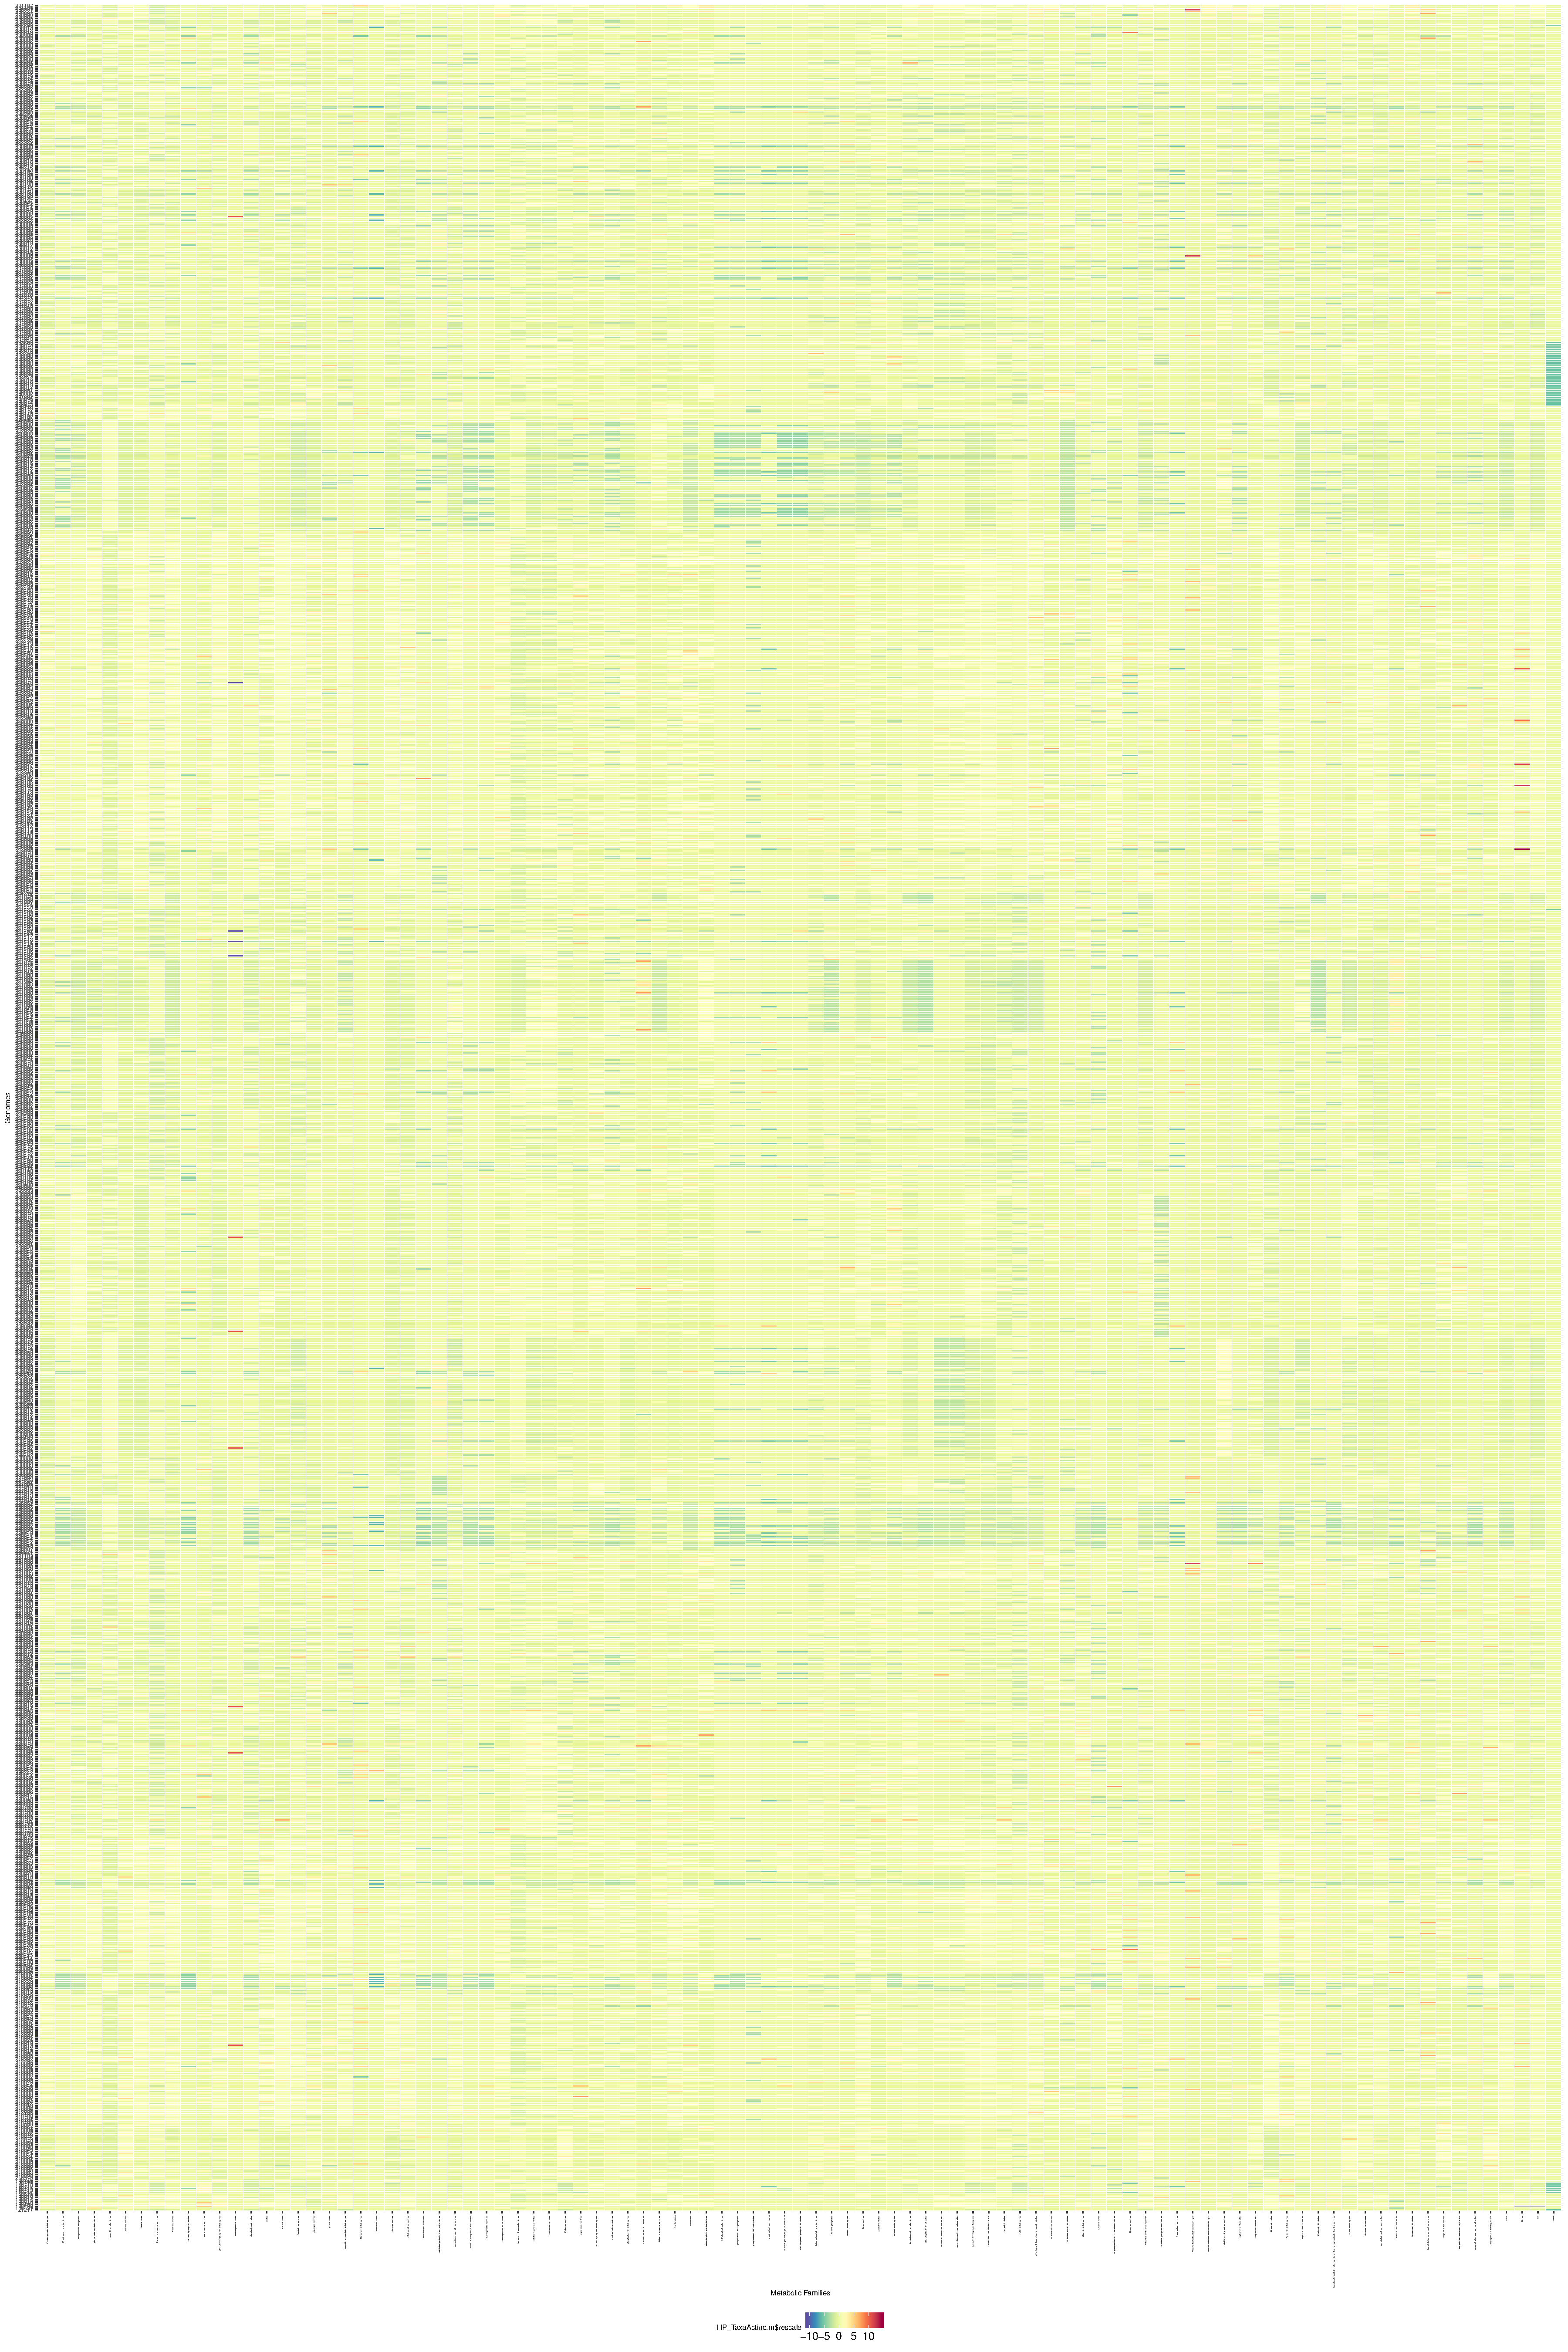
\includegraphics[angle = 0,scale = 0.7]{chapter4/HeatPlotActinos.pdf}
  \caption[Actinobacterial Heatplot]{\normalsize{Actinobacterial Heatplot}}
  \label{fig:ActinoPlot}
  \end{figure}
  
  Here is a reference to the HeatPlot: \autoref{fig:ActinoPlot}.
  \clearpage 
  
  PPP pahtway expansions restricted to \emph{Streptomycetaceae} family
  HeatPlot: \autoref{fig:ActinoPlot}.
  
  \begin{figure}[h!tbp]
  \centering
  
\includegraphics[angle = 0,scale = 0.7]{chapter4/HeatPlotStreptoPGA.pdf}
  \caption[Streptomyces Genomes expansions on PGA Aminoacids HeatPlot]{\normalsize{Streptomyces Genomes expansions on PGA Aminoacids HeatPlot}}
  \label{fig:StreptoPGAPlot}
  \end{figure}
  
  Here is a reference to the HeatPlot: \autoref{fig:StreptoPGAPlot}.
  \clearpage 
  
  \section{Genome Size correlations}\label{genome-size-correlations-1}
  
  \subsection{Correlation between genome size and AntiSMASH
  products}\label{correlation-between-genome-size-and-antismash-products-1}
  
  \begin{verbatim}
  Warning: Removed 1 rows containing missing values (geom_point).
  
  Warning: Removed 1 rows containing missing values (geom_point).
  \end{verbatim}
  
  Genome size vs Total antismash cluster coloured by order
  
  \begin{figure}[h!tbp]
  \centering
  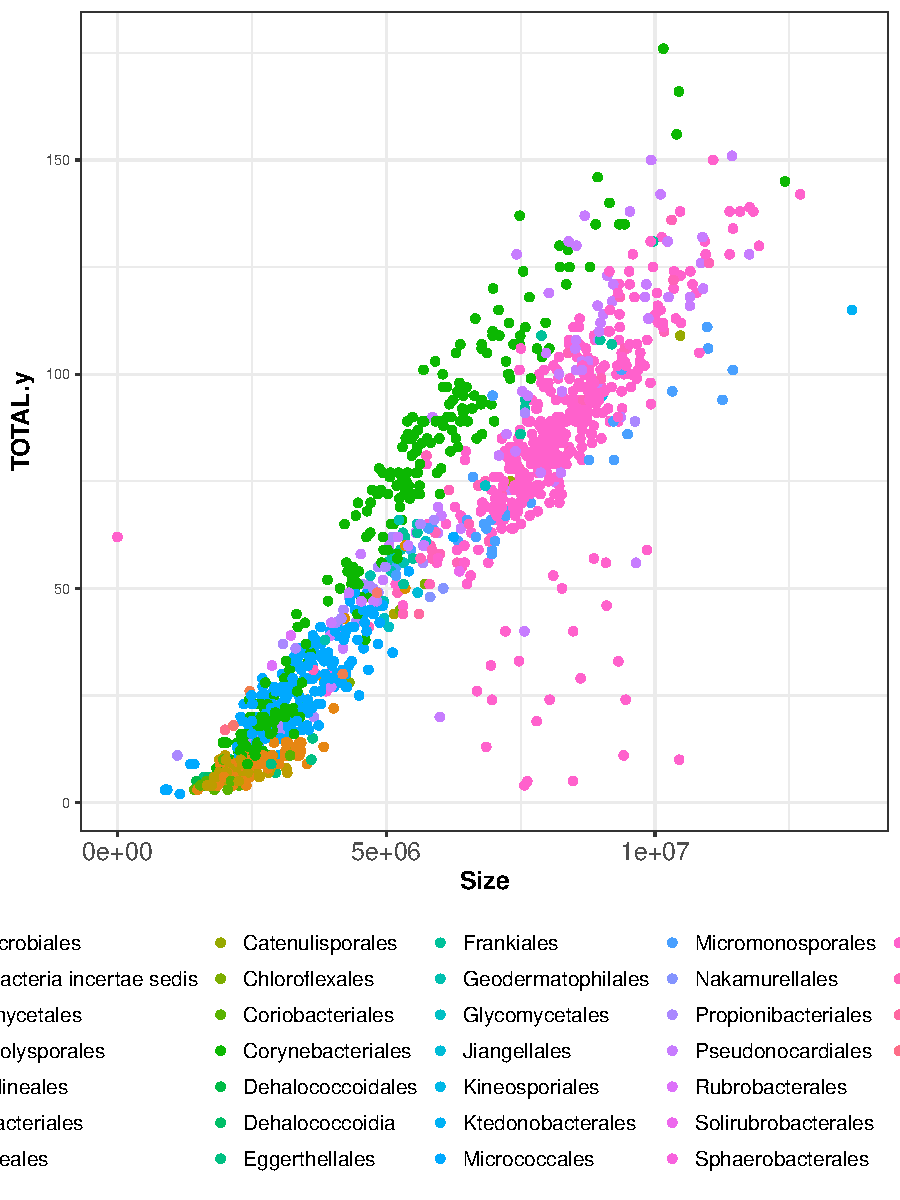
\includegraphics[angle = 0,scale = 0.6]{chapter4/ActinosSMASHvsSizebyOrder.pdf}
  \caption[Correlation between Actinos genome size and antismash Natural products detection colored by Order]{\normalsize{Correlation between Actinos genome size and antismash Natural products detection colored by Order}}
  \label{fig:ActinosSMASHvsSizebyOrder}
  \end{figure}
  
  Here is a reference to Genome size vs Total antismash cluster:
  \autoref{fig:ActinosSMASHvsSizebyOrder}. \clearpage
  
  Genome size vs Total antismash cluster detected splitted by order
  
  \begin{figure}[h!tbp]
  \centering
  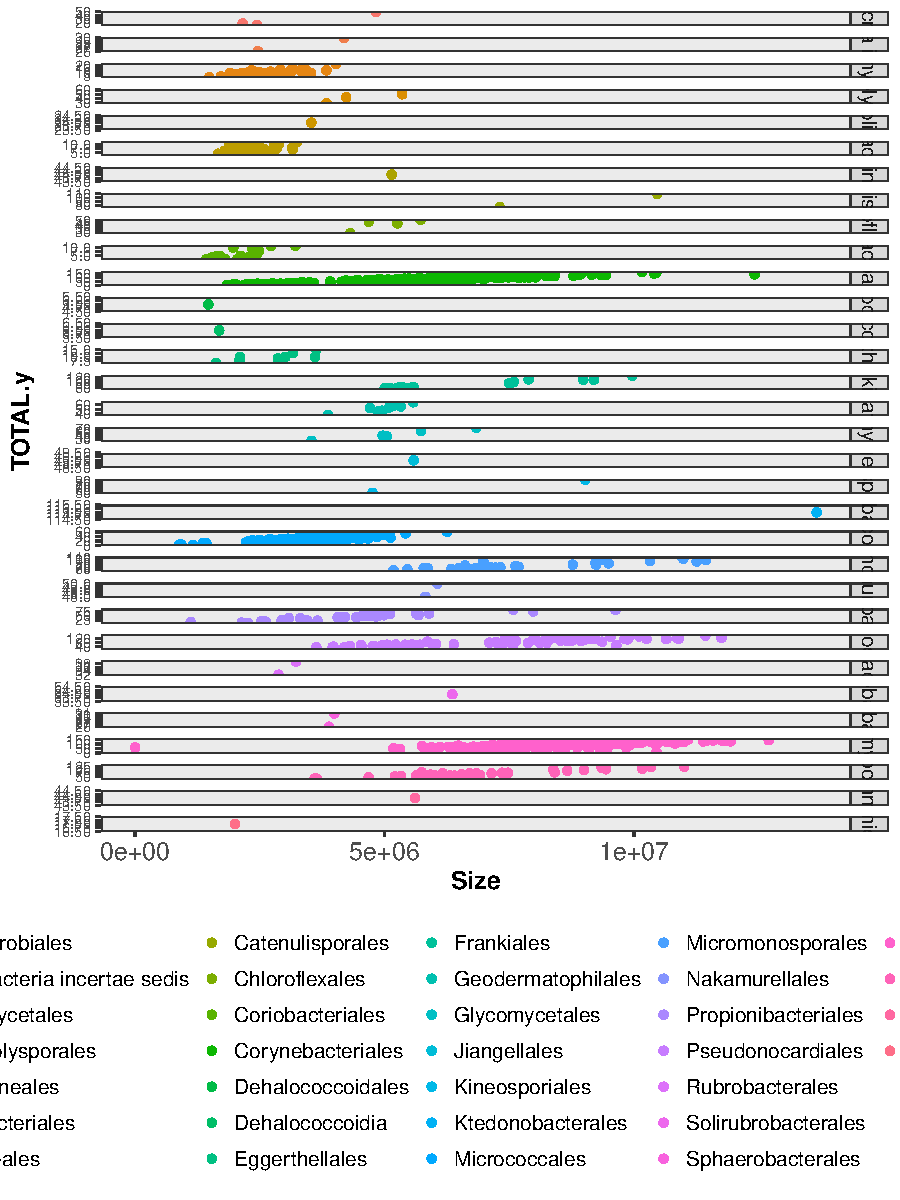
\includegraphics[angle = 0,scale = 0.6]{chapter4/ActinosSMASHvsSizeGridOrder.pdf}
  \caption[Correlation between Actinos genome size and antismash Natural products detection grided by Order]{\normalsize{Correlation between Actinos genome size and antismash Natural products detection grided by Order}}
  \label{fig:ActinosSMASHvsSizeGridOrder}
  \end{figure}
  
  Here is a reference to Correlation between genome size and antismash
  Natural products detection grided by Order plot:
  \autoref{fig:ActinosSMASHvsSizeGridOrder}. \clearpage 
  
  \subsection{Correlation between genome size and Central pathway
  expansions}\label{correlation-between-genome-size-and-central-pathway-expansions-1}
  
  \begin{verbatim}
  Warning: Removed 1 rows containing missing values (geom_point).
  
  Warning: Removed 1 rows containing missing values (geom_point).
  \end{verbatim}
  
  Genome size vs Total central pathway expansion coloured by order
  
  \begin{figure}[h!tbp]
  \centering
  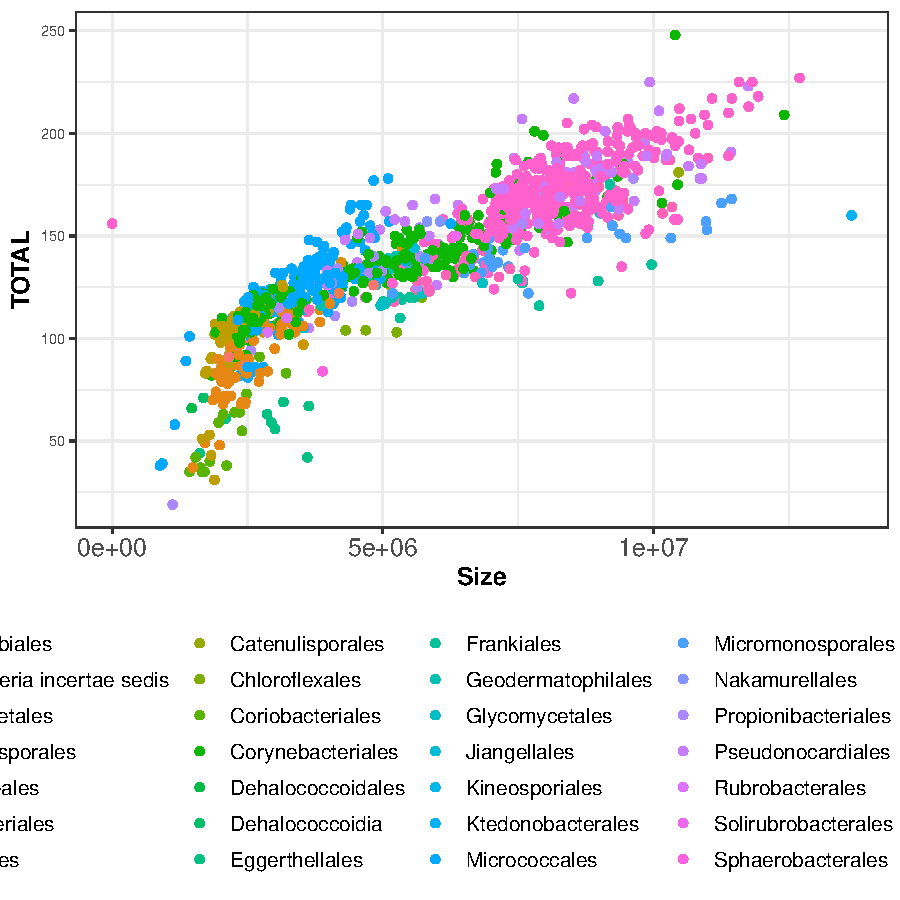
\includegraphics[angle = 0,scale = 1]{chapter4/ActinosSizevsExpansionsbyOrder.pdf}
  \caption[Correlation between Actinos genome size and central pathway expansions ]{\normalsize{Correlation between Actinos genome size and central pathway expansions }}
  \label{fig:ActinosSizevsExpansionsbyOrder}
  \end{figure}
  
  Here is a reference to the size vs Total central pathway expansion plot:
  \autoref{fig:ActinosSizevsExpansionsbyOrder}. \clearpage 
  
  Genome size vs Total central pathway expansion grided by order
  
  \begin{figure}[h!tbp]
  \centering
  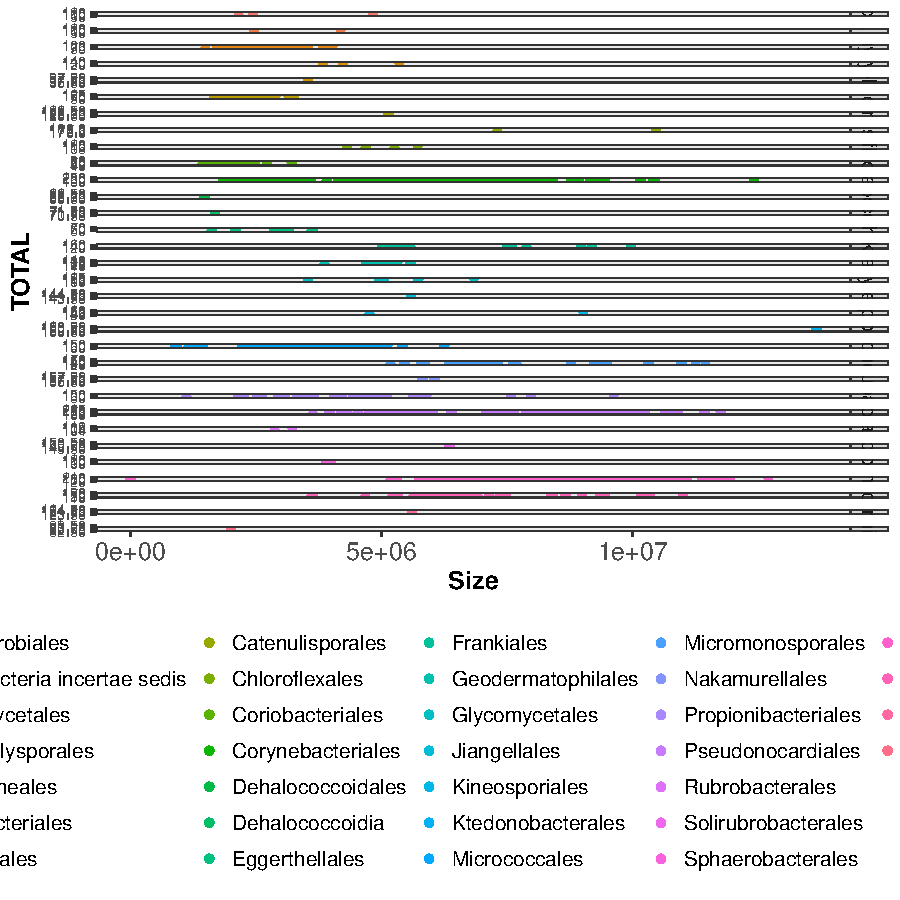
\includegraphics[angle = 0,scale = 1]{chapter4/ActinosSizevsExpansionsGridbyOrder.pdf}
  \caption[Correlation between Actinos genome size and central pathway expansions grided by order]{\normalsize{Correlation between Actinos genome size and central pathway expansions grided by order}}
  \label{fig:ActinosSizevsExpansionsGridbyOrder}
  \end{figure}
  
  Here is a reference to the Genome size vs Total central pathway
  expansion grided by order plot:
  \autoref{fig:ActinosSizevsExpansionsGridbyOrder}. \clearpage 
  
  Correlation between genome size and each of the central pathway
  families. Data are coloured by metabolic family instead of coloured by
  taxonomical order. This treatment allows to answer how differente
  metabolic families grows when genome size grow.\\
  Also I want to add form given by taxonomical order.
  
  \begin{verbatim}
  Warning: The shape palette can deal with a maximum of 6 discrete values
  because more than 6 becomes difficult to discriminate; you have
  32. Consider specifying shapes manually if you must have them.
  \end{verbatim}
  
  \begin{verbatim}
  Warning: Removed 103306 rows containing missing values (geom_point).
  \end{verbatim}
  
  \begin{verbatim}
  Warning: Removed 94 rows containing missing values (geom_point).
  \end{verbatim}
  
  Genome size vs Total central pathway expansion coloured by metabolic
  Family
  
  \begin{figure}[h!tbp]
  \centering
  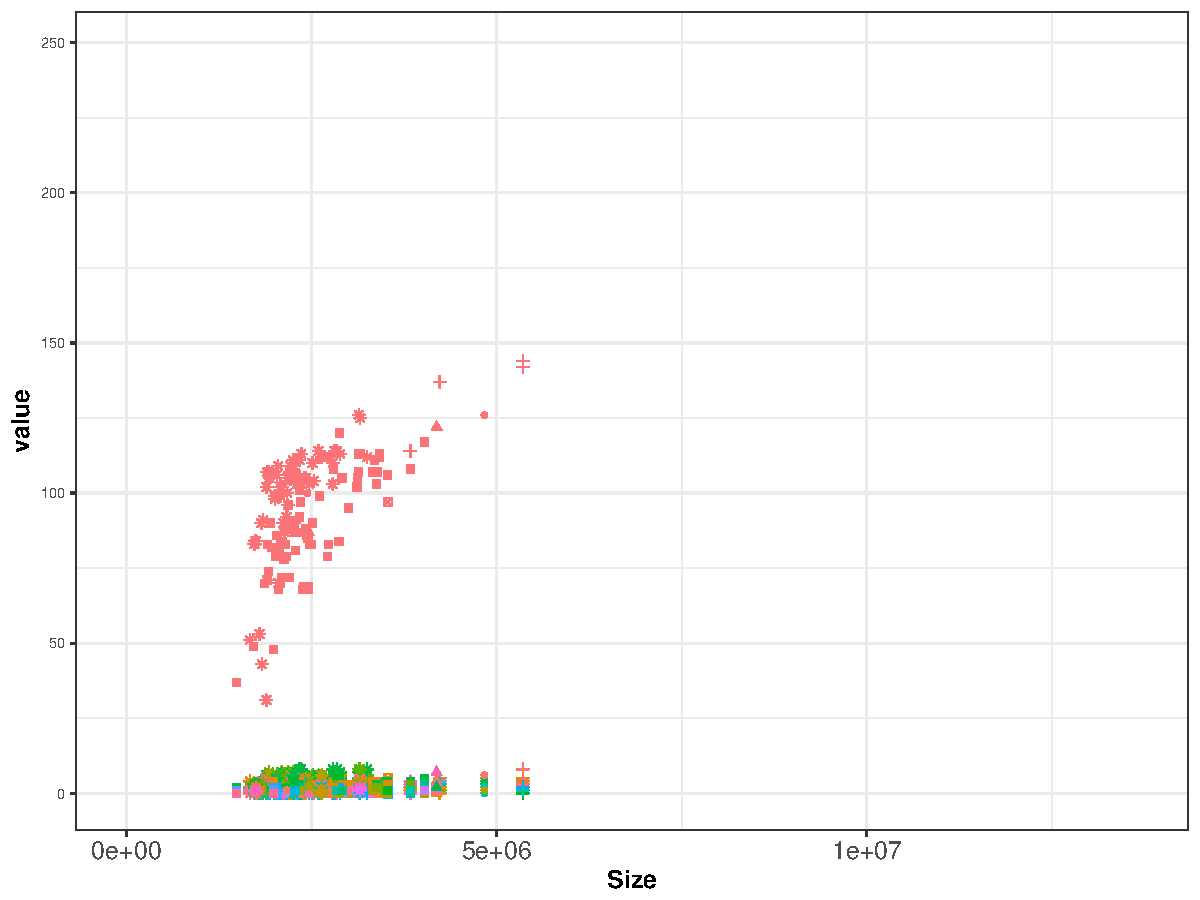
\includegraphics[angle = 0,scale = 0.6]{chapter4/ActinosSizevsExpansionsbyMetabolicFamily.pdf}
  \caption[Correlation between Actinos Genome size vs Total central pathway expansion coloured by metabolic Family]{\normalsize{Correlation between Actinos Genome size vs Total central pathway expansion coloured by metabolic Family}}
  \label{fig:ActinosSizevsExpansionsbyMetabolicFamily}
  \end{figure}
  
  Here is a reference to the Genome size vs Total central pathway
  expansion coloured by metabolic Family plot:
  \autoref{fig:ActinosSizevsExpansionsbyMetabolicFamily}. \clearpage 
  
  Future Work: Genome size vs Total central pathway expansion grided by
  metabolic Family For clarity I need to also grid and group by Metabolic
  Pathway
  
  Here is a reference to Genome size vs Total central pathway expansion
  grided by metabolic Family plot:
  \autoref{fig:ActinosExpansionsbyMetabolicFamilyGrid}. \clearpage 
  
  \section{Natural products}\label{natural-products-1}
  
  \subsection{Natural products recruitments from EvoMining
  heatplot}\label{natural-products-recruitments-from-evomining-heatplot-1}
  
  We can see natural products recruitment after central pathways
  expansions colored by their kingdom.\\
  Natural products recruited by metabolic family, colored by phylogenetic
  origin.
  
  Recruitments after central pathways expansions coloured by Kingdom
  
  \begin{figure}[h!tbp]
  \centering
  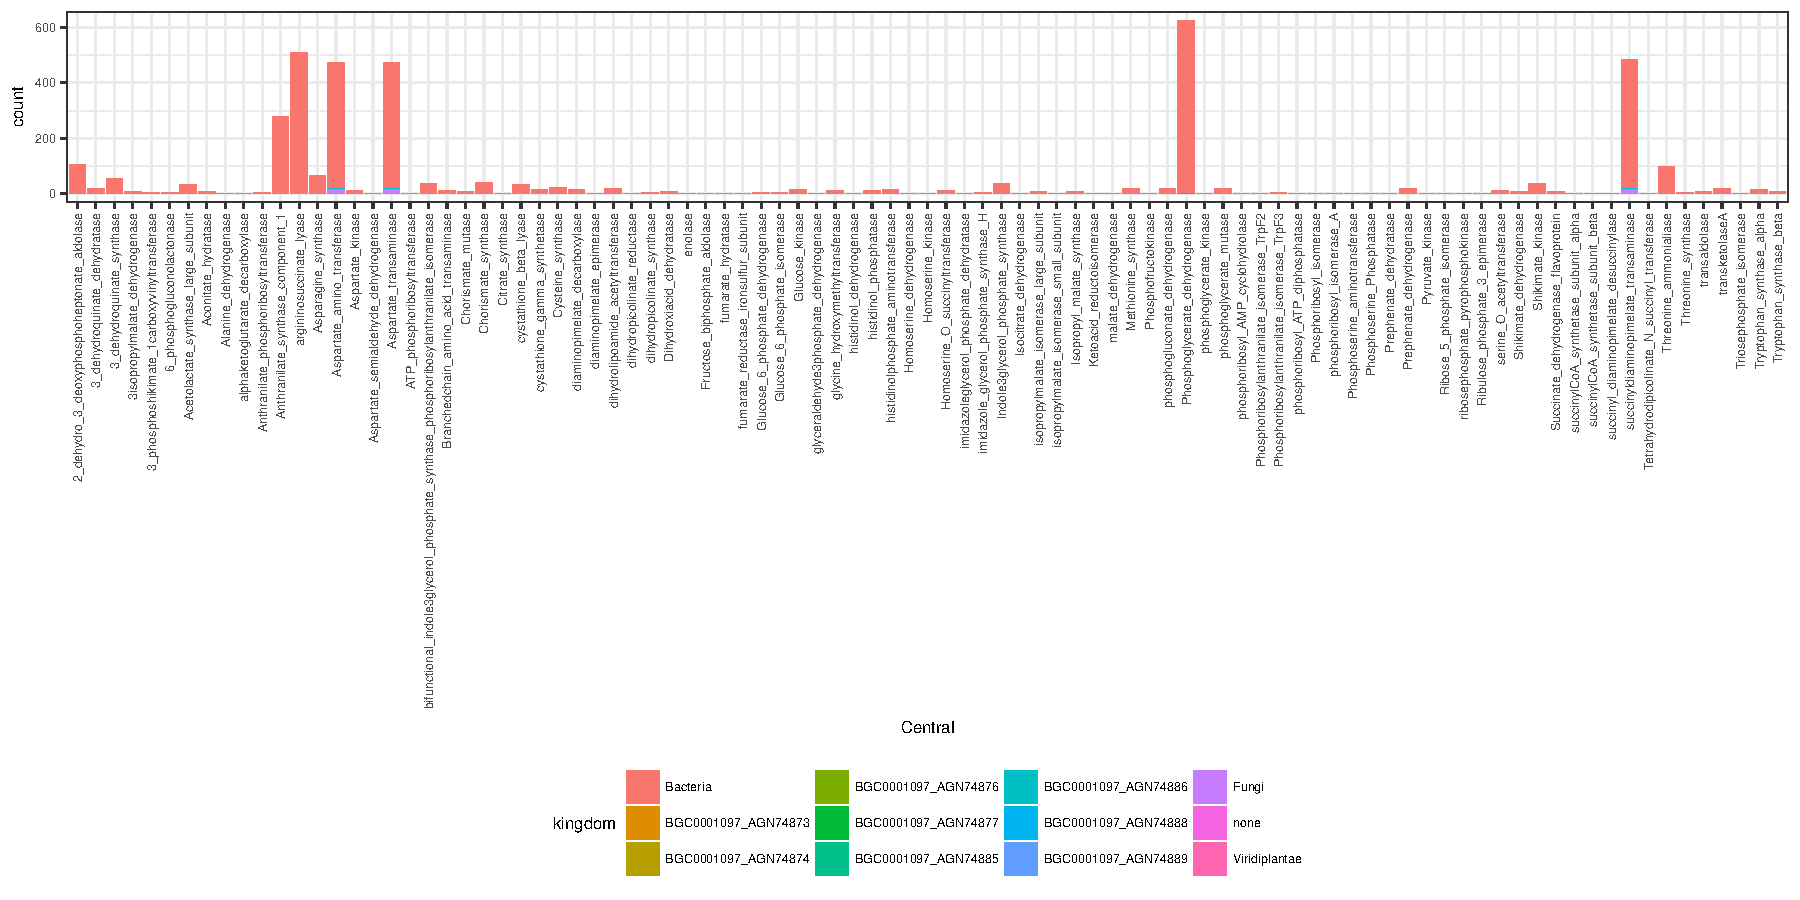
\includegraphics[angle = 0,scale = 0.6]{chapter4/ActinosRecruitmentsbyKingdom.pdf}
  \caption[Actinos Recruitmens on central families coloured by kingdom]{\normalsize{Actinos Recruitmens on central families coloured by kingdom}}
  \label{fig:ActinosRecruitmentsbyKingdom}
  \end{figure}
  
  Here is a reference to Recruitments after central pathways expansions
  colourd by Kingdom plot: \autoref{fig:ActinosRecruitmentsbyKingdom}.
  
  \clearpage 
  Recruitments after central pathways expansions colourd by taxonomy
  
  \begin{figure}[h!tbp]
  \centering
  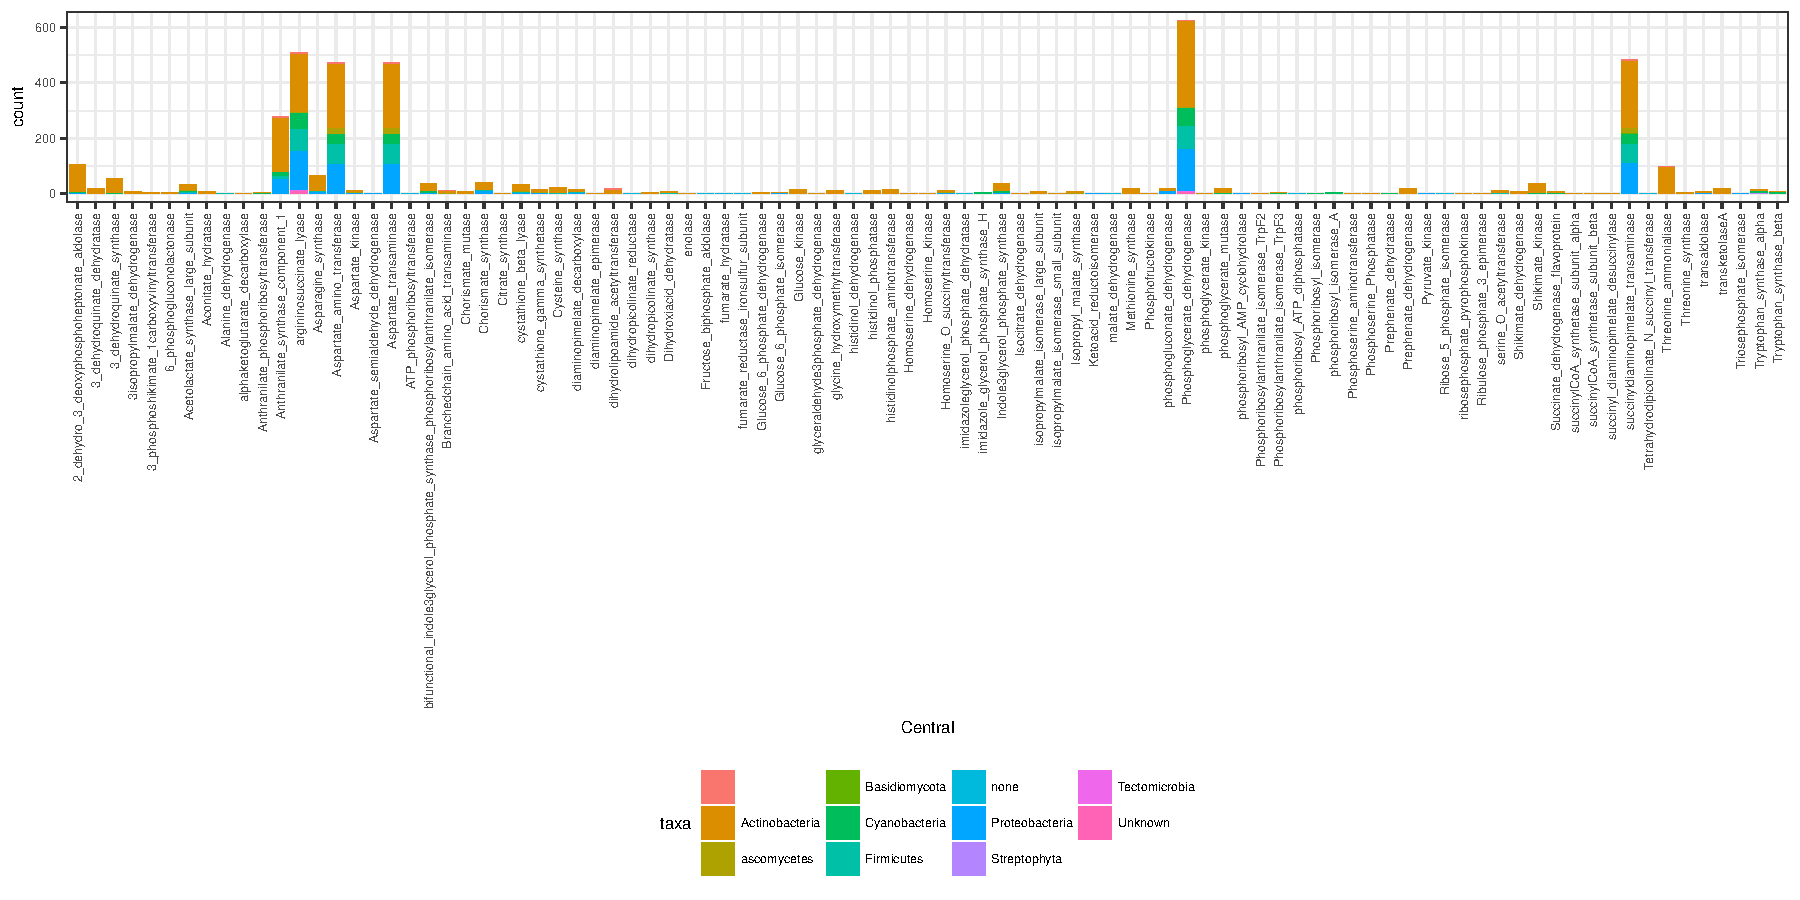
\includegraphics[angle = 0,scale = 0.5]{chapter4/ActinosRecruitmentsbyTaxa.pdf}
  \caption[Actinos Recruitmens on central families coloured by taxonomy]{\normalsize{Actinos Recruitmens on central families coloured by taxonomy}}
  \label{fig:ActinosRecruitmentsbyTaxa}
  \end{figure}
  
  Here is a reference to Recruitments after central pathways expansions
  colourd by taxa plot: \autoref{fig:ActinosRecruitmentsbyTaxa}.
  \clearpage 
  
  \section{Actinos AntiSMASH}\label{actinos-antismash}
  
  Taxonomical diversity on Actinosbacteria Data
  
  \begin{figure}[h!tbp]
  \centering
  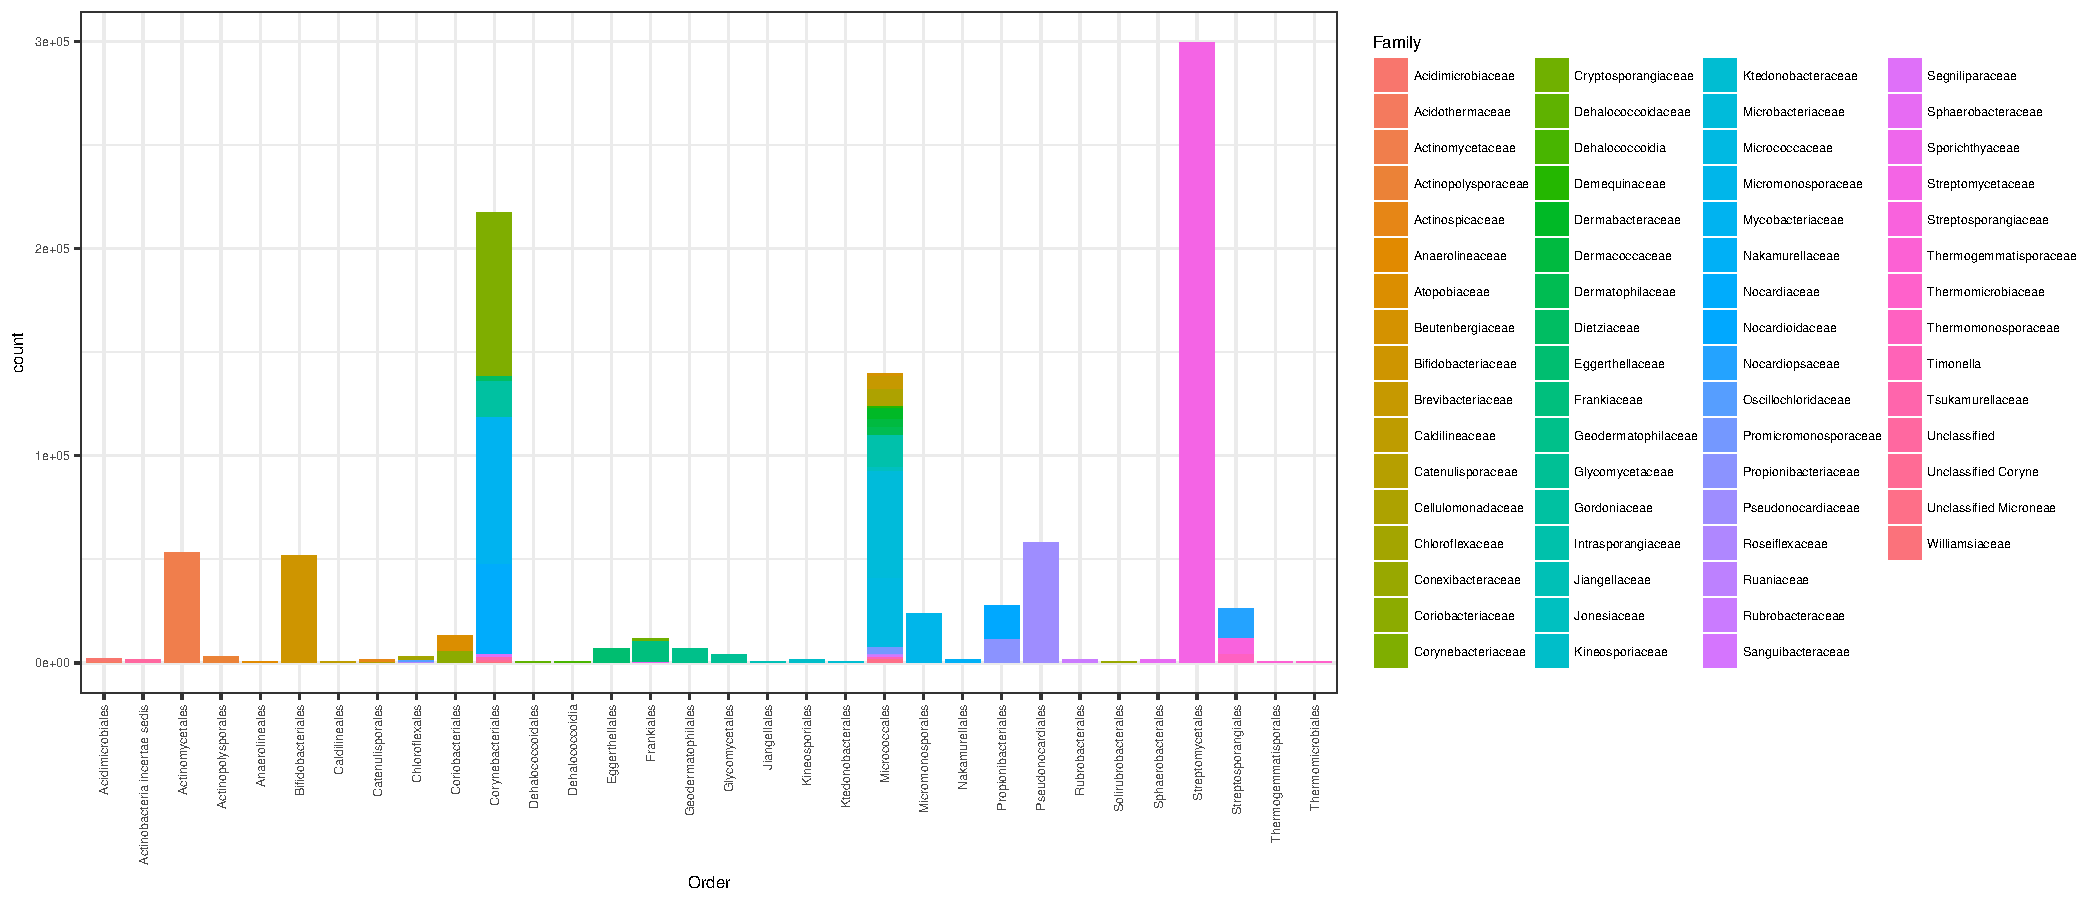
\includegraphics[angle = 0,scale = 0.6]{chapter4/ActinosDiversity.pdf}
  \caption[Actinos Diversity]{\normalsize{Actinos Diversity}}
  \label{fig:ActinosDiversity}
  \end{figure}
  
  Here is a reference to Recruitments after central pathways expansions
  colourd by taxa plot: \autoref{fig:ActinosDiversity}. \clearpage
  
  Smash diversity
  
  \begin{figure}[h!tbp]
  \centering
  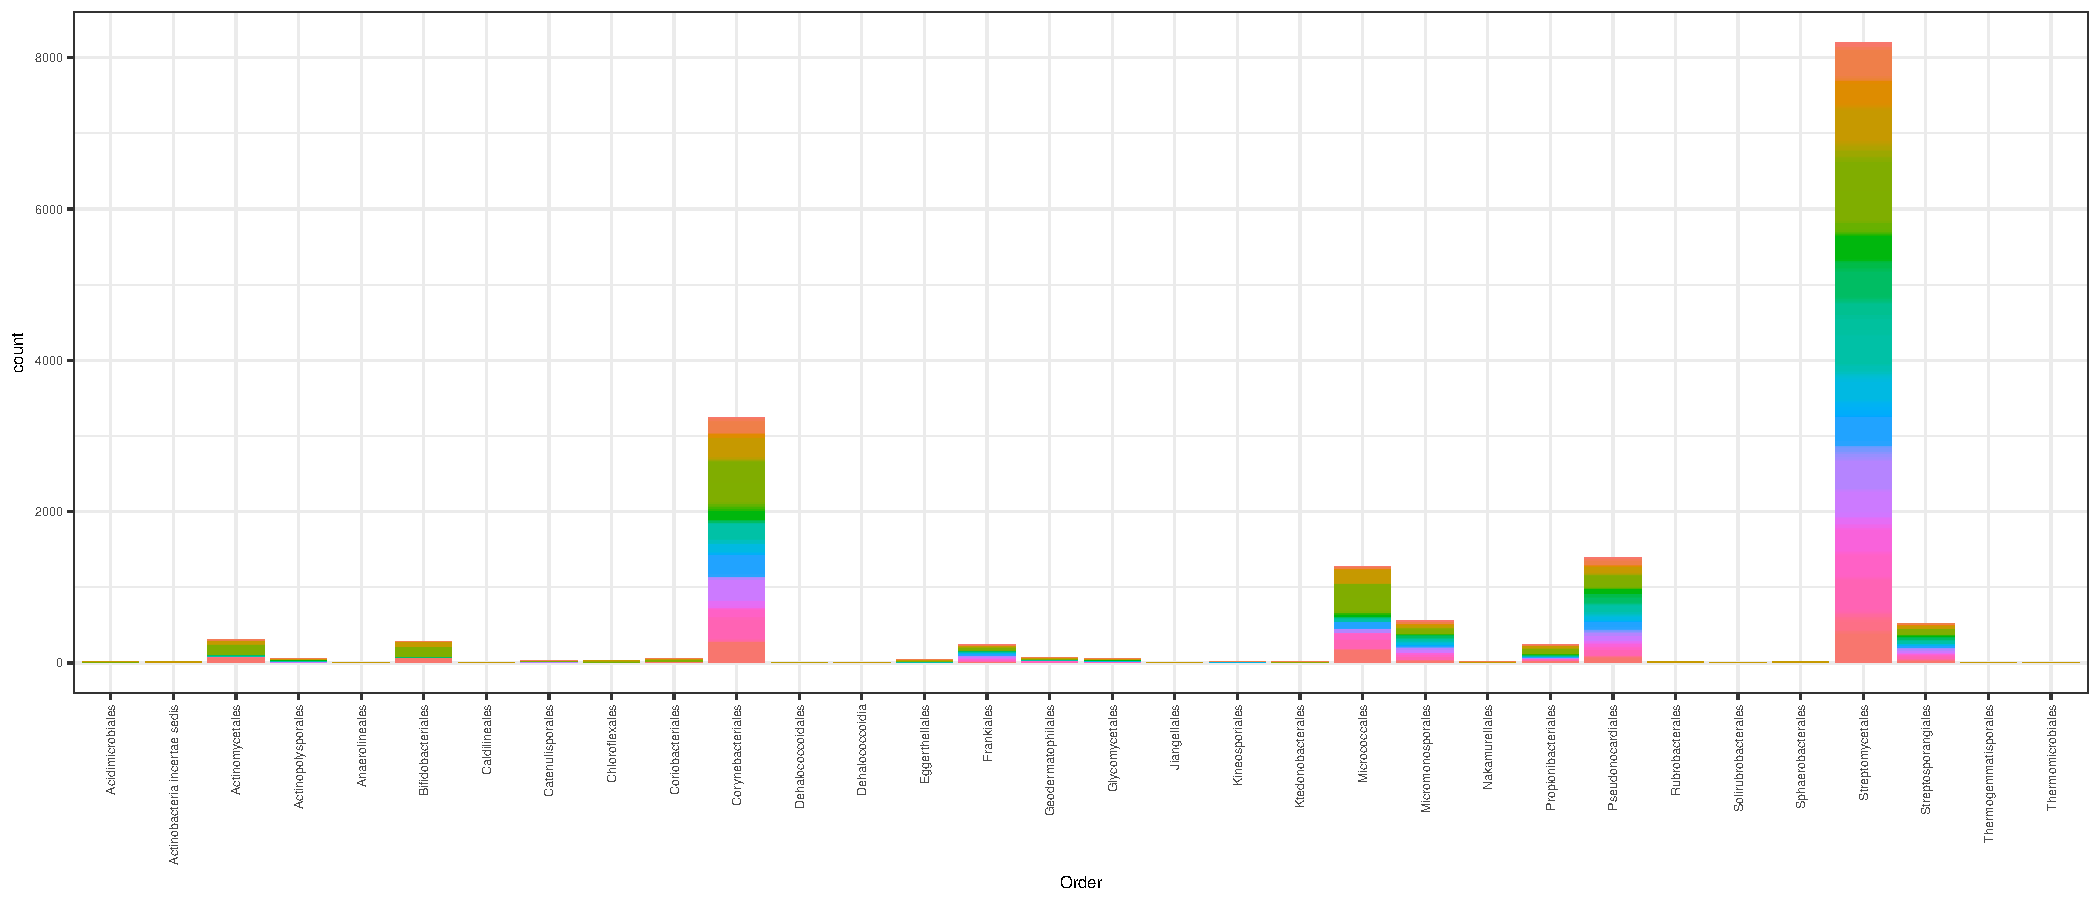
\includegraphics[angle = 0,scale = 0.5]{chapter4/ActinosSmash.pdf}
  \caption[Actinos Smash Taxonomical Diversity]{\normalsize{Actinos Smash Taxonomical Diversity}}
  \label{fig:ActinosSmash}
  \end{figure}
  
  Here is a reference to Recruitments after central pathways expansions
  colourd by taxa plot: \autoref{fig:ActinosSmash}. \clearpage
  
  \subsection{AntisSMASH vs Central
  Expansions}\label{antissmash-vs-central-expansions-1}
  
  Is it a correlation between pangenome grow and central pathways
  expansions?
  
  Total central pathway expansions by genome vs Total antismash cluster
  detected coloured by order
  
  \begin{figure}[h!tbp]
  \centering
  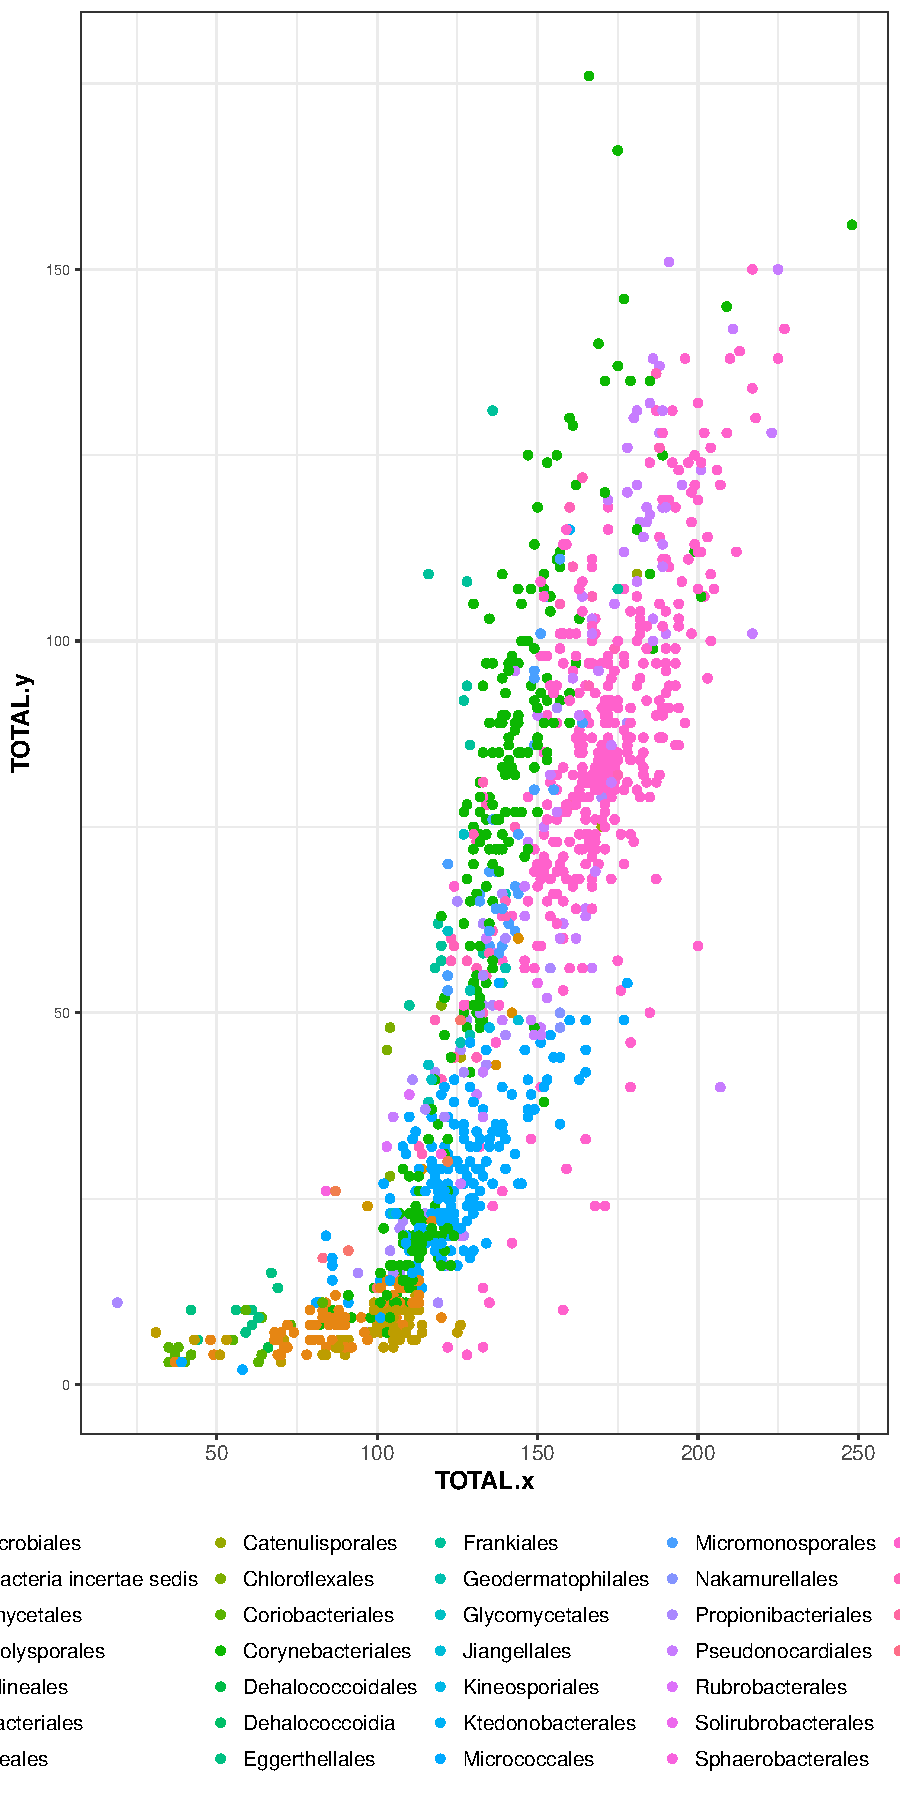
\includegraphics[angle = 0,scale = 0.5]{chapter4/ActinosSMASHvsExpansionsbyOrder.pdf}
  \caption[Correlation between Actinos central pathway expansions and antismash Natural products detection]{\normalsize{Correlation between Actinos central pathway expansions and antismash Natural products detection}}
  \label{fig:ActinosSMASHvsExpansionsbyOrder}
  \end{figure}
  
  Here is a reference to the expansions vs antismash NP's clusters plot:
  \autoref{fig:ActinosSMASHvsExpansionsbyOrder}. \clearpage 
  
  Total central pathway expansions by genome vs Total antismash cluster
  detected splitted by order
  
  \begin{figure}[h!tbp]
  \centering
  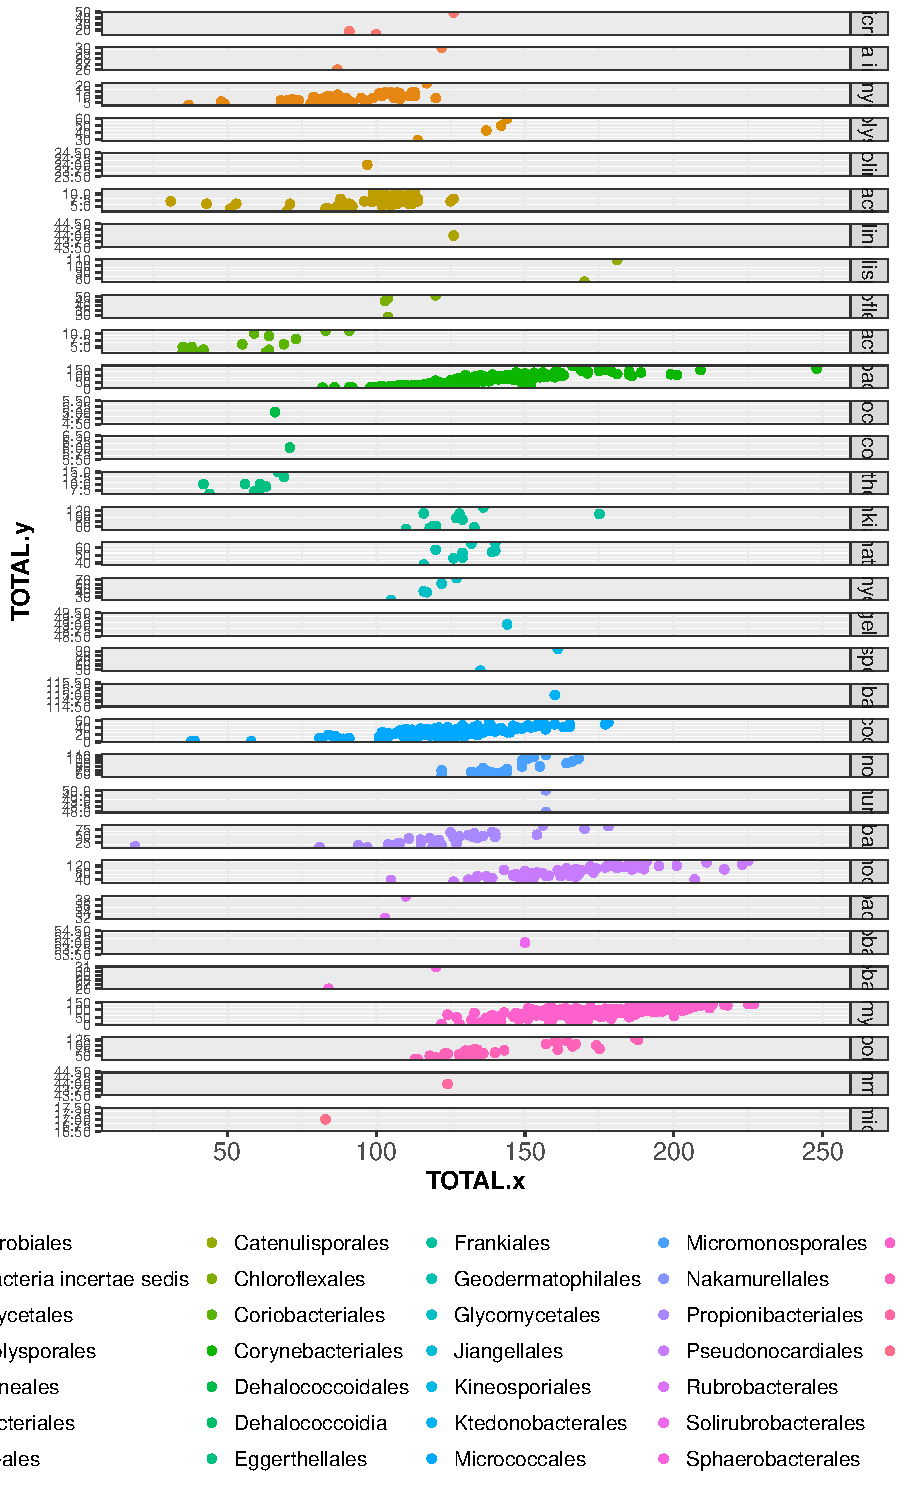
\includegraphics[angle = 0,scale = 0.5]{chapter4/ActinosSMASHvsExpansionsbyOrderGRID.pdf}
  \caption[Correlation between Actinos central pathway expnasions and antismash Natural products detection]{\normalsize{Correlation between Actinos central pathway expnasions and antismash Natural products detection}}
  \label{fig:ActinosSMASHvsExpansionsbyOrderGRID}
  \end{figure}
  
  Here is a reference to the expansions vs antismash NP's clusters
  splitted by order plot
  \autoref{fig:ActinosSMASHvsExpansionsbyOrderGRID}. \clearpage 
  
  AntisMAsh vs Expansions by taxonomic Family
  
  Natural products colured by family
  
  \begin{figure}[h!tbp]
  \centering
  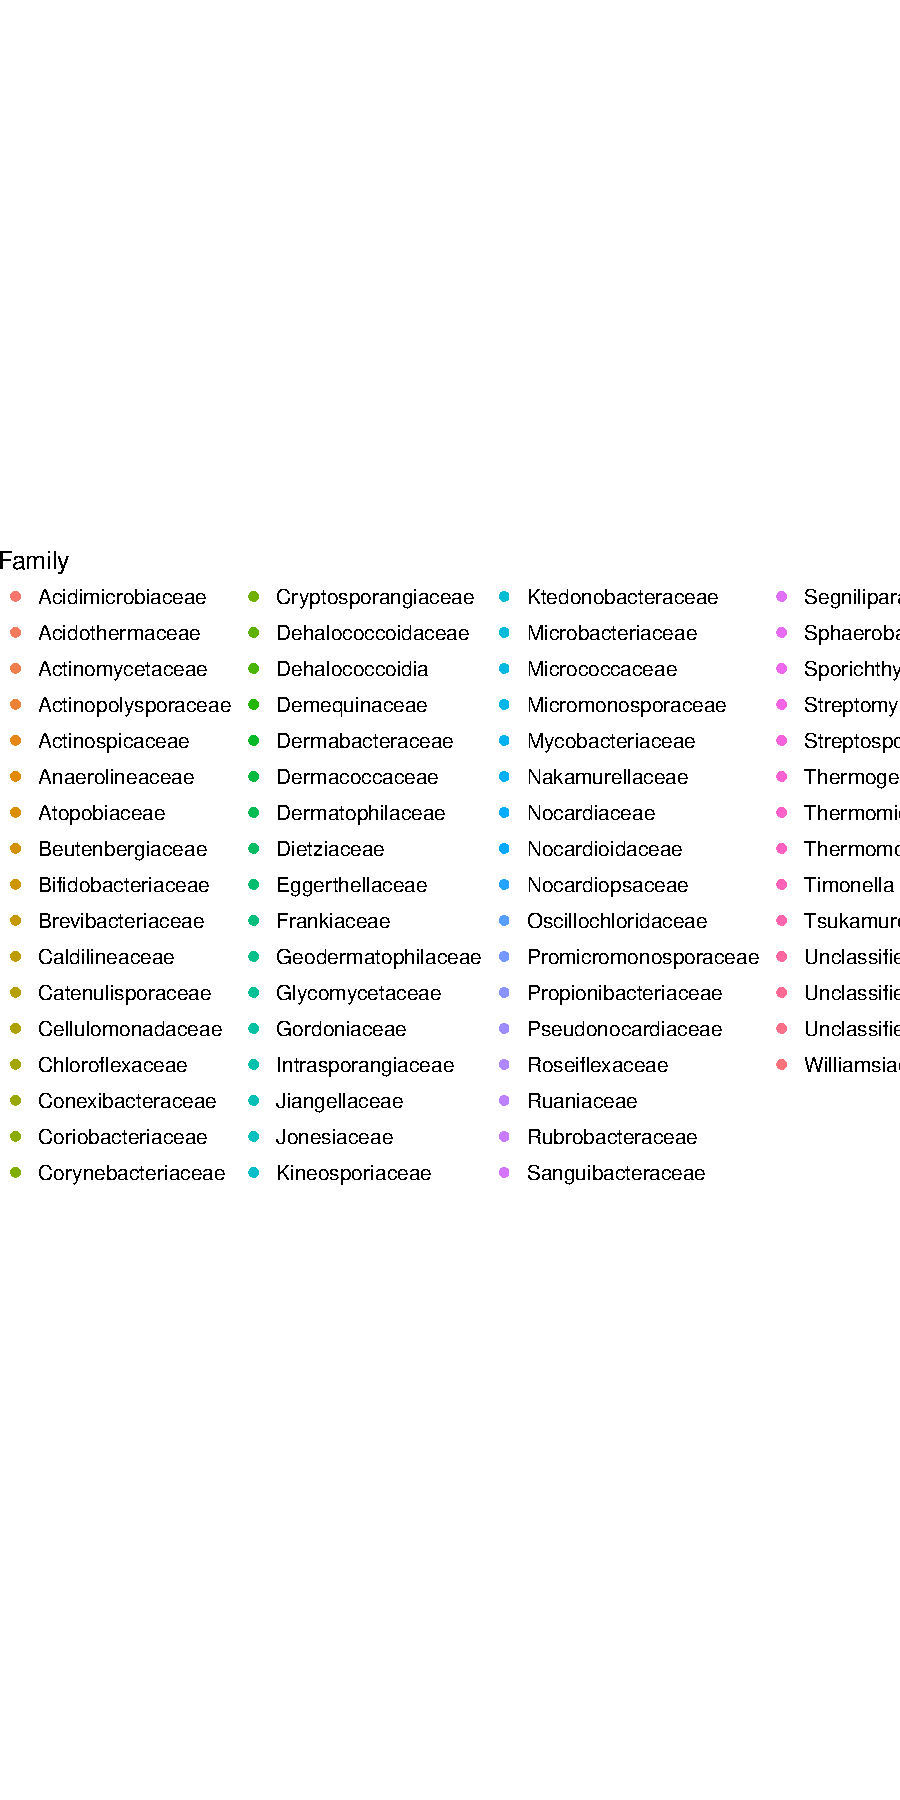
\includegraphics[angle = 0,scale = 0.6]{chapter4/Actinosnpf.pdf}
  \caption[Actinos Natural products by family]{\normalsize{Actinos Natural products by family}}
  \label{fig:Actinosnpf}
  \end{figure}
  
  Here is a reference to the Natural products colured by family plot
  \autoref{fig:Actinosnpf}. \clearpage 
  
  \section{Selected trees from
  EvoMining}\label{selected-trees-from-evomining-1}
  
  \begin{figure}[h!tbp]
  \centering
  \includegraphics[angle = 180,scale = 0.3]{chapter4/tree15.png}
  \caption[Enolase EvoMiningtree]{\normalsize{Enolase EvoMiningtree}}
  \label{fig:enolase_evo_tree}
  \end{figure}\begin{figure}[h!tbp]
  \centering
  \includegraphics[angle = 180,scale = 0.3]{chapter4/tree73.png}
  \caption[Phosphoribosyl isomerase EvoMiningtree]{\normalsize{Phosphoribosyl isomerase EvoMiningtree}}
  \label{fig:Phosphoribosyl_isomerase_evo_tree}
  \end{figure}\begin{figure}[h!tbp]
  \centering
  \includegraphics[angle = 180,scale = 0.3]{chapter4/tree47.png}
  \caption[Phosphoribosyl isomerase A EvoMiningtree]{\normalsize{Phosphoribosyl isomerase A EvoMiningtree}}
  \label{fig:Phosphoribosyl_isomerase_A_evo_tree}
  \end{figure}\begin{figure}[h!tbp]
  \centering
  \includegraphics[angle = 180,scale = 0.3]{chapter4/tree69.png}
  \caption[phosphoshikimate carboxyvinyltransferase EvoMiningtree]{\normalsize{phosphoshikimate carboxyvinyltransferase EvoMiningtree}}
  \label{fig:phosphoshikimate_c_evo_tree}
  \end{figure}
  
  \clearpage 
  
  \hypertarget{refux5flabels}{\chapter{Cyanobacteria EvoMining
  Results}\label{refux5flabels}}
  
  Cyanobacteria phylum \{Referencia\}\\
  Cyanobacteria is a photosynthetic phylum that inhabits a broad range of
  habitats. The broad adaptive potential is on part driven by gene-family
  enlargment {[}\protect\hyperlink{ref-larssonux5fgenomeux5f2011}{128}{]}
  by the analysis of 58 Cyanobacterial genomes concludes ancestor of
  cyanobacteria had a genome size of approx. 4.5 Mbp. Cyanobacteria
  produces natural products as pigments and toxins
  {[}\protect\hyperlink{ref-whittonux5fecologyux5f2012}{129}{]} Example of
  a PriA cluster
  toxins{[}\protect\hyperlink{ref-moustafaux5foriginux5f2009}{94}{]}
  
  Fossil record situates Cyanobacteria
  {[}\protect\hyperlink{ref-whittonux5fecologyux5f2012}{129}{]} Molecular
  record and metabolic propoerties at
  {[}\protect\hyperlink{ref-battistuzziux5fgenomicux5f2004}{132}{]}
  
  \section{Tables}\label{tables-2}
  
  \begin{longtable}[c]{@{}cc@{}}
  \caption{Families on Cyanobacteria \label{tab:inher}}\tabularnewline
  \toprule
  Factors & Correlation between Parents \& Child\tabularnewline
  \midrule
  \endfirsthead
  \toprule
  Factors & Correlation between Parents \& Child\tabularnewline
  \midrule
  \endhead
  GenomeDB & 1245\tabularnewline
  Families & 65\tabularnewline
  \bottomrule
  \end{longtable}
  
  \clearpage
  
  \subsection{Expansions BoxPlot by metabolic
  family}\label{expansions-boxplot-by-metabolic-family-2}
  
  \begin{Shaded}
  \begin{Highlighting}[]
  \KeywordTok{label}\NormalTok{(}\DataTypeTok{path =} \StringTok{"chapter5/expansion_plotCyanos.pdf"}\NormalTok{, }\DataTypeTok{caption =} \StringTok{"Expansions Boxplot"}\NormalTok{,}\DataTypeTok{label =} \StringTok{"Cyano_expansion_boxplot"}\NormalTok{, }\DataTypeTok{type =} \StringTok{"figure"}\NormalTok{)}
  \end{Highlighting}
  \end{Shaded}
  
  \begin{figure}[h!tbp]
  \centering
  \includegraphics[angle = 0,scale = 1]{chapter5/expansion_plotCyanos.pdf}
  \caption[Expansions Boxplot]{\normalsize{Expansions Boxplot}}
  \label{fig:Cyano_expansion_boxplot}
  \end{figure}
  
  Here is a reference to the expansion boxplot:
  \autoref{fig:Cyano_expansion_boxplot}.\\
  \clearpage 
  
  \section{Central pathway expansions}\label{central-pathway-expansions-2}
  
  Heat plot of central pathways expansions, Needs to be phylogenetically
  sorted.
  
  \begin{figure}[h!tbp]
  \centering
  \includegraphics[angle = 0,scale = 0.6]{chapter5/HeatPlot.pdf}
  \caption[Cyanobacterial Heatplot]{\normalsize{Cyanobacterial Heatplot}}
  \label{fig:CyanoPlot}
  \end{figure}
  
  Here is a reference to the HeatPlot: \autoref{fig:CyanoPlot}.
  \clearpage 
  
  \section{Genome Size correlations}\label{genome-size-correlations-2}
  
  \subsection{Correlation between genome size and AntiSMASH
  products}\label{correlation-between-genome-size-and-antismash-products-2}
  
  Genome size vs Total antismash cluster coloured by order
  
  \begin{figure}[h!tbp]
  \centering
  \includegraphics[angle = 0,scale = 0.6]{chapter5/SMASHvsSizebyOrder.pdf}
  \caption[Correlation between genome size and antismash Natural products detection colored by Order]{\normalsize{Correlation between genome size and antismash Natural products detection colored by Order}}
  \label{fig:SMASHvsSizebyOrder}
  \end{figure}
  
  Here is a reference to Genome size vs Total antismash cluster:
  \autoref{fig:SMASHvsSizebyOrder}. \clearpage
  
  Genome size vs Total antismash cluster detected splitted by order
  
  \begin{figure}[h!tbp]
  \centering
  \includegraphics[angle = 0,scale = 0.6]{chapter5/SMASHvsSizeGridOrder.pdf}
  \caption[Correlation between genome size and antismash Natural products detection grided by Order]{\normalsize{Correlation between genome size and antismash Natural products detection grided by Order}}
  \label{fig:SMASHvsSizeGridOrder}
  \end{figure}
  
  Here is a reference to Correlation between genome size and antismash
  Natural products detection grided by Order plot:
  \autoref{fig:SMASHvsSizeGridOrder}. \clearpage 
  
  \subsection{Correlation between genome size and Central pathway
  expansions}\label{correlation-between-genome-size-and-central-pathway-expansions-2}
  
  Genome size vs Total central pathway expansion coloured by order
  
  \begin{figure}[h!tbp]
  \centering
  \includegraphics[angle = 0,scale = 1]{chapter5/SizevsExpansionsbyOrder.pdf}
  \caption[Correlation between genome size and central pathway expansions ]{\normalsize{Correlation between genome size and central pathway expansions }}
  \label{fig:SizevsExpansionsbyOrder}
  \end{figure}
  
  Here is a reference to the size vs Total central pathway expansion plot:
  \autoref{fig:SizevsExpansionsbyOrder}. \clearpage 
  
  Genome size vs Total central pathway expansion grided by order
  
  \begin{figure}[h!tbp]
  \centering
  \includegraphics[angle = 0,scale = 1]{chapter5/SizevsExpansionsGridbyOrder.pdf}
  \caption[Correlation between genome size and central pathway expansions grided by order]{\normalsize{Correlation between genome size and central pathway expansions grided by order}}
  \label{fig:SizevsExpansionsGridbyOrder}
  \end{figure}
  
  Here is a reference to the Genome size vs Total central pathway
  expansion grided by order plot:
  \autoref{fig:SizevsExpansionsGridbyOrder}. \clearpage 
  
  Correlation between genome size and each of the central pathway
  families. Data are coloured by metabolic family instead of coloured by
  taxonomical order. This treatment allows to answer how differente
  metabolic families grows when genome size grow.\\
  Also I want to add form given by taxonomical order.
  
  \begin{verbatim}
  Warning: The shape palette can deal with a maximum of 6 discrete values
  because more than 6 becomes difficult to discriminate; you have
  10. Consider specifying shapes manually if you must have them.
  \end{verbatim}
  
  \begin{verbatim}
  Warning: Removed 20418 rows containing missing values (geom_point).
  \end{verbatim}
  
  Genome size vs Total central pathway expansion coloured by metabolic
  Family
  
  \begin{figure}[h!tbp]
  \centering
  \includegraphics[angle = 0,scale = 0.6]{chapter5/SizevsExpansionsbyMetabolicFamily.pdf}
  \caption[Correlation between Genome size vs Total central pathway expansion coloured by metabolic Family]{\normalsize{Correlation between Genome size vs Total central pathway expansion coloured by metabolic Family}}
  \label{fig:SizevsExpansionsbyMetabolicFamily}
  \end{figure}
  
  Here is a reference to the Genome size vs Total central pathway
  expansion coloured by metabolic Family plot:
  \autoref{fig:SizevsExpansionsbyMetabolicFamily}. \clearpage 
  
  Future Work: Genome size vs Total central pathway expansion grided by
  metabolic Family For clarity I need to also grid and group by Metabolic
  Pathway
  
  Here is a reference to Genome size vs Total central pathway expansion
  grided by metabolic Family plot:
  \autoref{fig:ExpansionsbyMetabolicFamilyGrid}. \clearpage 
  
  \section{Natural products}\label{natural-products-2}
  
  \subsection{Natural products recruitments from EvoMining
  heatplot}\label{natural-products-recruitments-from-evomining-heatplot-2}
  
  We can see natural products recruitment after central pathways
  expansions colored by their kingdom.\\
  Natural products recruited by metabolic family, colored by phylogenetic
  origin.
  
  Recruitments after central pathways expansions coloured by Kingdom
  
  \begin{figure}[h!tbp]
  \centering
  \includegraphics[angle = 0,scale = 0.6]{chapter5/RecruitmentsbyKingdom.pdf}
  \caption[Recruitmens on central families coloured by kingdom]{\normalsize{Recruitmens on central families coloured by kingdom}}
  \label{fig:RecruitmentsbyKingdom}
  \end{figure}
  
  Here is a reference to Recruitments after central pathways expansions
  colourd by Kingdom plot: \autoref{fig:RecruitmentsbyKingdom}.
  
  \clearpage 
  Recruitments after central pathways expansions colourd by taxonomy
  
  \begin{figure}[h!tbp]
  \centering
  \includegraphics[angle = 0,scale = 0.5]{chapter5/RecruitmentsbyTaxa.pdf}
  \caption[Recruitmens on central families coloured by taxonomy]{\normalsize{Recruitmens on central families coloured by taxonomy}}
  \label{fig:RecruitmentsbyTaxa}
  \end{figure}
  
  Here is a reference to Recruitments after central pathways expansions
  colourd by taxa plot: \autoref{fig:RecruitmentsbyTaxa}. \clearpage 
  
  \section{Cyanobacterias AntiSMASH}\label{cyanobacterias-antismash}
  
  Taxonomical diversity on Cyanobacteria Data
  
  \begin{figure}[h!tbp]
  \centering
  \includegraphics[angle = 0,scale = 0.6]{chapter5/Diversity.pdf}
  \caption[Diversity]{\normalsize{Diversity}}
  \label{fig:Diversity}
  \end{figure}
  
  Here is a reference to Recruitments after central pathways expansions
  colourd by taxa plot: \autoref{fig:Diversity}. \clearpage
  
  Smash diversity
  
  \begin{figure}[h!tbp]
  \centering
  \includegraphics[angle = 0,scale = 0.5]{chapter5/Smash.pdf}
  \caption[Smash]{\normalsize{Smash}}
  \label{fig:Smash Taxonomical Diversity}
  \end{figure}
  
  Here is a reference to Recruitments after central pathways expansions
  colourd by taxa plot: \autoref{fig:Smash}. \clearpage
  
  \subsection{AntisSMASH vs Central
  Expansions}\label{antissmash-vs-central-expansions-2}
  
  Is it a correlation between pangenome grow and central pathways
  expansions?
  
  Total central pathway expansions by genome vs Total antismash cluster
  detected coloured by order
  
  \begin{figure}[h!tbp]
  \centering
  \includegraphics[angle = 0,scale = 0.5]{chapter5/SMASHvsExpansionsbyOrder.pdf}
  \caption[Correlation between central pathway axpnasions and antismash Natural products detection]{\normalsize{Correlation between central pathway axpnasions and antismash Natural products detection}}
  \label{fig:SMASHvsExpansionsbyOrder}
  \end{figure}
  
  Here is a reference to the expansions vs antismash NP's clusters plot:
  \autoref{fig:SMASHvsExpansionsbyOrder}. \clearpage 
  
  Total central pathway expansions by genome vs Total antismash cluster
  detected splitted by order
  
  \begin{figure}[h!tbp]
  \centering
  \includegraphics[angle = 0,scale = 0.5]{chapter5/SMASHvsExpansionsbyOrderGRID.pdf}
  \caption[Correlation between central pathway axpnasions and antismash Natural products detection]{\normalsize{Correlation between central pathway axpnasions and antismash Natural products detection}}
  \label{fig:SMASHvsExpansionsbyOrderGRID}
  \end{figure}
  
  Here is a reference to the expansions vs antismash NP's clusters
  splitted by order plot \autoref{fig:SSMASHvsExpansionsbyOrderGRID}.
  \clearpage 
  
  AntisMAsh vs Expansions by taxonomic Family
  
  Natural products colured by family
  
  \begin{figure}[h!tbp]
  \centering
  \includegraphics[angle = 0,scale = 0.6]{chapter5/npf.pdf}
  \caption[Natural products by family]{\normalsize{Natural products by family}}
  \label{fig:npf}
  \end{figure}
  
  Here is a reference to the Natural products colured by family plot
  \autoref{fig:npf}. \clearpage 
  
  \section{Selected trees from
  EvoMining}\label{selected-trees-from-evomining-2}
  
  Phosphoribosyl\_isomerase\_3 family\\
  Figure from EvoMining
  
  \begin{figure}[h!tbp]
  \centering
  \includegraphics[angle = 180,scale = 0.25]{chapter5/tree64.png}
  \caption[Phosphoribosyl isomerase EvoMiningtree]{\normalsize{Phosphoribosyl isomerase EvoMiningtree}}
  \label{fig:Phosphoribosyl_isomerase_evo_tree}
  \end{figure}\begin{figure}[h!tbp]
  \centering
  \includegraphics[angle = 180,scale = 0.25]{chapter5/tree1.png}
  \caption[Phosphoglycerate dehydrogenase EvoMiningtree]{\normalsize{Phosphoglycerate dehydrogenase EvoMiningtree}}
  \label{fig:Phosphoglycerate_dehydrogenase_evo_tree}
  \end{figure}\begin{figure}[h!tbp]
  \centering
  \includegraphics[angle = 180,scale = 0.25]{chapter5/tree2.png}
  \caption[Phosphoserine aminotransferase EvoMiningtree]{\normalsize{Phosphoserine aminotransferase EvoMiningtree}}
  \label{fig:Phosphoserine_aminotransferase_evo_tree}
  \end{figure}\begin{figure}[h!tbp]
  \centering
  \includegraphics[angle = 180,scale = 0.25]{chapter5/tree10.png}
  \caption[Triosephosphate isomerase EvoMiningtree]{\normalsize{Triosephosphate isomerase EvoMiningtree}}
  \label{fig:Triosephosphate_isomerase_evo_tree}
  \end{figure}\begin{figure}[h!tbp]
  \centering
  \includegraphics[angle = 180,scale = 0.25]{chapter5/tree11.png}
  \caption[glyceraldehyde3phosphate dehydrogenase EvoMiningtree]{\normalsize{glyceraldehyde3phosphate dehydrogenase EvoMiningtree}}
  \label{fig:glyceraldehyde3phosphate_dehydrogenase_evo_tree}
  \end{figure}\begin{figure}[h!tbp]
  \centering
  \includegraphics[angle = 180,scale = 0.25]{chapter5/tree12.png}
  \caption[phosphoglycerate kinase EvoMiningtree]{\normalsize{phosphoglycerate kinase EvoMiningtree}}
  \label{fig:phosphoglycerate_kinase_evo_tree}
  \end{figure}\begin{figure}[h!tbp]
  \centering
  \includegraphics[angle = 180,scale = 0.25]{chapter5/tree13.png}
  \caption[phosphoglycerate mutaseEvoMiningtree]{\normalsize{phosphoglycerate mutaseEvoMiningtree}}
  \label{fig:phosphoglycerate_mutase_evo_tree}
  \end{figure}\begin{figure}[h!tbp]
  \centering
  \includegraphics[angle = 180,scale = 0.25]{chapter5/tree14.png}
  \caption[enolase EvoMiningtree]{\normalsize{enolase EvoMiningtree}}
  \label{fig:enolase_evo_tree}
  \end{figure}\begin{figure}[h!tbp]
  \centering
  \includegraphics[angle = 180,scale = 0.25]{chapter5/tree15.png}
  \caption[Pyruvate kinase EvoMiningtree]{\normalsize{Pyruvate kinase EvoMiningtree}}
  \label{fig:Pyruvate_kinase_evo_tree}
  \end{figure}\begin{figure}[h!tbp]
  \centering
  \includegraphics[angle = 180,scale = 0.25]{chapter5/tree16.png}
  \caption[Aspartate transaminase EvoMiningtree]{\normalsize{Aspartate transaminase EvoMiningtree}}
  \label{fig:Aspartate_transaminase_evo_tree}
  \end{figure}\begin{figure}[h!tbp]
  \centering
  \includegraphics[angle = 180,scale = 0.25]{chapter5/tree17.png}
  \caption[Asparagine synthase EvoMiningtree]{\normalsize{Asparagine synthase EvoMiningtree}}
  \label{fig:Asparagine_synthase_evo_tree}
  \end{figure}\begin{figure}[h!tbp]
  \centering
  \includegraphics[angle = 180,scale = 0.25]{chapter5/tree18.png}
  \caption[Aspartate kinase EvoMiningtree]{\normalsize{Aspartate kinase EvoMiningtree}}
  \label{fig:Aspartate_kinase_evo_tree}
  \end{figure}\begin{figure}[h!tbp]
  \centering
  \includegraphics[angle = 180,scale = 0.25]{chapter5/tree19.png}
  \caption[Aspartate semialdehyde dehydrogenase EvoMiningtree]{\normalsize{Aspartate semialdehyde dehydrogenase EvoMiningtree}}
  \label{fig:Aspartate_semialdehyde_dehydrogenase_evo_tree}
  \end{figure}\begin{figure}[h!tbp]
  \centering
  \includegraphics[angle = 180,scale = 0.25]{chapter5/tree20.png}
  \caption[Homoserine dehydrogenase EvoMiningtree]{\normalsize{Homoserine dehydrogenase EvoMiningtree}}
  \label{fig:Homoserine_dehydrogenase_evo_tree}
  \end{figure}
  
  \clearpage 
  
  \chapter*{Conclusion}\label{conclusion}
  \addcontentsline{toc}{chapter}{Conclusion}
  
  \setcounter{chapter}{4} \setcounter{section}{0}
  
  Idea de Rosario -ver dell cluster de saxitoxin cuantos pasos se
  necesitron para llegar ahi.\\
  -A donde se iria el resultado de abrir el GMP\\
  -Otra vez, que Actinos tienen FolE
  
  If we don't want Conclusion to have a chapter number next to it, we can
  add the \texttt{\{.unnumbered\}} attribute. This has an unintended
  consequence of the sections being labeled as 3.6 for example though
  instead of 4.1. The \LaTeX~commands immediately following the Conclusion
  declaration get things back on track.
  
  \subsubsection{More info}\label{more-info}
  
  And here's some other random info: the first paragraph after a chapter
  title or section head \emph{shouldn't be} indented, because indents are
  to tell the reader that you're starting a new paragraph. Since that's
  obvious after a chapter or section title, proper typesetting doesn't add
  an indent there.
  
  \appendix
  
  \chapter{The First Appendix}\label{the-first-appendix}
  
  This first appendix includes all of the R chunks of code that were
  hidden throughout the document (using the \texttt{include\ =\ FALSE}
  chunk tag) to help with readibility and/or setup.
  
  \subsubsection{In the main Rmd file:}\label{in-the-main-rmd-file}
  
  \begin{Shaded}
  \begin{Highlighting}[]
  \CommentTok{# This chunk ensures that the reedtemplates package is}
  \CommentTok{# installed and loaded. This reedtemplates package includes}
  \CommentTok{# the template files for the thesis and also two functions}
  \CommentTok{# used for labeling and referencing}
  \NormalTok{if(!}\KeywordTok{require}\NormalTok{(devtools))}
    \KeywordTok{install.packages}\NormalTok{(}\StringTok{"devtools"}\NormalTok{, }\DataTypeTok{repos =} \StringTok{"http://cran.rstudio.com"}\NormalTok{)}
  \NormalTok{if(!}\KeywordTok{require}\NormalTok{(reedtemplates))\{}
    \KeywordTok{library}\NormalTok{(devtools)}
    \NormalTok{devtools::}\KeywordTok{install_github}\NormalTok{(}\StringTok{"ismayc/reedtemplates"}\NormalTok{)}
  \NormalTok{\}}
  \KeywordTok{library}\NormalTok{(reedtemplates)}
  \end{Highlighting}
  \end{Shaded}
  
  \subsubsection{\texorpdfstring{In
  \protect\hyperlink{refux5flabels}{}:}{In :}}\label{in}
  
  \begin{Shaded}
  \begin{Highlighting}[]
  \CommentTok{# This chunk ensures that the reedtemplates package is}
  \CommentTok{# installed and loaded. This reedtemplates package includes}
  \CommentTok{# the template files for the thesis and also two functions}
  \CommentTok{# used for labeling and referencing}
  \NormalTok{if(!}\KeywordTok{require}\NormalTok{(devtools))}
    \KeywordTok{install.packages}\NormalTok{(}\StringTok{"devtools"}\NormalTok{, }\DataTypeTok{repos =} \StringTok{"http://cran.rstudio.com"}\NormalTok{)}
  \NormalTok{if(!}\KeywordTok{require}\NormalTok{(plyr))}
      \KeywordTok{install.packages}\NormalTok{(}\StringTok{"plyr"}\NormalTok{, }\DataTypeTok{repos =} \StringTok{"http://cran.rstudio.com"}\NormalTok{)}
  \NormalTok{if(!}\KeywordTok{require}\NormalTok{(dplyr))}
      \KeywordTok{install.packages}\NormalTok{(}\StringTok{"dplyr"}\NormalTok{, }\DataTypeTok{repos =} \StringTok{"http://cran.rstudio.com"}\NormalTok{)}
  \NormalTok{if(!}\KeywordTok{require}\NormalTok{(ggplot2))}
      \KeywordTok{install.packages}\NormalTok{(}\StringTok{"ggplot2"}\NormalTok{, }\DataTypeTok{repos =} \StringTok{"http://cran.rstudio.com"}\NormalTok{)}
  \NormalTok{if(!}\KeywordTok{require}\NormalTok{(reedtemplates))\{}
    \KeywordTok{library}\NormalTok{(devtools)}
    \NormalTok{devtools::}\KeywordTok{install_github}\NormalTok{(}\StringTok{"ismayc/reedtemplates"}\NormalTok{)}
    \NormalTok{\}}
  \KeywordTok{library}\NormalTok{(reedtemplates)}
  \NormalTok{flights <-}\StringTok{ }\KeywordTok{read.csv}\NormalTok{(}\StringTok{"data/flights.csv"}\NormalTok{)}
  \end{Highlighting}
  \end{Shaded}
  
  \chapter{The Second Appendix, Open source code on this
  document}\label{the-second-appendix-open-source-code-on-this-document}
  
  \section{R markdown}\label{r-markdown}
  
  Thanks to Rmakdown Thesis\\
  Apendix one Useful docker commands\\
  -Create a new repository\\
  \texttt{docker\ build\ .\ -t\ evomining}\\
  \texttt{docker\ push\ nselemevomining}
  
  \section{Docker}\label{docker}
  
  Restart docker and free all ports\\
  \texttt{sudo\ service\ docker\ restart}
  
  liast containers\\
  \texttt{docker\ ps\ -a}
  
  ssh or bash into a running docker container\\
  \texttt{sudo\ docker\ exec\ -i\ -t\ romantic\_brahmagupta\ /bin/bash}
  \texttt{docker\ exec\ -it\ \textless{}mycontainer\textgreater{}\ bash}
  
  Stop all containers\\
  \texttt{docker\ rm\ \$(docker\ ps\ -a\ -q)}
  
  Remove stopped containers\\
  \texttt{docker\ rm\ \$(docker\ ps\ -q\ -f\ status=exited)}
  
  Remove all images\\
  \texttt{docker\ rmi\ \$(docker\ images\ -q)}
  
  uninstall docker from ubuntu (Fresh start)\\
  \texttt{sudo\ apt-get\ purge\ docker-engine}\\
  \texttt{sudo\ apt-get\ autoremove\ -\/-purge\ docker-engine}\\
  \texttt{rm\ -rf\ /var/lib/docker} \# This deletes all images,
  containers, and volumes
  
  Run Evomining container using nselem/newevomining image\\
  \texttt{docker\ run\ -i\ -t\ -v\ /home/nelly/GIT/EvoMining/:/var/www/html/EvoMining/exchange\ -p\ 80:80\ nselem/newevomining\ /bin/bash}
  
  Start evomining inside this container\\
  \texttt{perl\ startevomining}
  
  Vizualice a tree\\
  \texttt{http://10.10.100.234/EvoMining/cgi-bin/color\_tree.pl?9\&\&/var/www/html/EvoMining/exchange/CyanosBBH\_MiBIG\_DB.faa\_CYANOS}
  file 9.new must be on folder volume CyanosBBH\_MiBIG\_DB.faa\_CYANOS
  
  Find a perl module\\
  \texttt{perl\ -MList::Util\ -e\textquotesingle{}print\ \$\_\ .\ "\ =\textgreater{}\ "\ .\ \$INC\{\$\_\}\ .\ "\textbackslash{}n"\ for\ keys\ \%INC\textquotesingle{}}
  EvoMining notes\\
  Gblocks only runs inside folder /var/www/html/EvoMining
  
  \section{Git}\label{git}
  
  \texttt{git\ add\ -\/-all}\\
  \texttt{git\ commit\ -m\ "Some\ message"}\\
  \texttt{git\ push\ -u\ origin\ master}\\
  \texttt{git\ clone}
  
  \section{Connect GitHub and
  DockerHub}\label{connect-github-and-dockerhub}
  
  automated builds The Dockerfile is available to anyone with access to
  your Docker Hub repository. Your repository is kept up-to-date with code
  changes automatically.
  
  \section{Additional resources}\label{additional-resources}
  
  \begin{itemize}
  \item
    \emph{Markdown} Cheatsheet -
    \url{https://github.com/adam-p/markdown-here/wiki/Markdown-Cheatsheet}
  \item
    \emph{R Markdown} Reference Guide -
    \url{https://www.rstudio.com/wp-content/uploads/2015/03/rmarkdown-reference.pdf}
  \item
    Introduction to \texttt{dplyr} -
    \url{https://cran.rstudio.com/web/packages/dplyr/vignettes/introduction.html}
  \item
    \texttt{ggplot2} Documentation -
    \url{http://docs.ggplot2.org/current/}
  \end{itemize}
  
  \backmatter
  
  \chapter{References}\label{references}
  
  \noindent
  
  \setlength{\parindent}{-0.20in} \setlength{\leftskip}{0.20in}
  \setlength{\parskip}{8pt}
  
  \hypertarget{refs}{}
  \hypertarget{ref-angel2000}{}
  1. Angel E. Interactive computer graphics : A top-down approach with
  openGL. Boston, MA: Addison Wesley Longman; 2000.
  
  \hypertarget{ref-angel2001}{}
  2. Angel E. Batch-file computer graphics : A bottom-up approach with
  quickTime. Boston, MA: Wesley Addison Longman; 2001.
  
  \hypertarget{ref-angel2002a}{}
  3. Angel E. Test second book by angel. Boston, MA: Wesley Addison
  Longman; 2001.
  
  \hypertarget{ref-khersonskyux5fenzymeux5f2010}{}
  4. Khersonsky O, Tawfik DS. Enzyme promiscuity: A mechanistic and
  evolutionary perspective. Annual Review of Biochemistry. 2010;79:
  471--505.
  doi:\href{https://doi.org/10.1146/annurev-biochem-030409-143718}{10.1146/annurev-biochem-030409-143718}
  
  \hypertarget{ref-copleyux5fenzymesux5f2003}{}
  5. Copley SD. Enzymes with extra talents: Moonlighting functions and
  catalytic promiscuity. Current Opinion in Chemical Biology. 2003;7:
  265--272.
  doi:\href{https://doi.org/10.1016/S1367-5931(03)00032-2}{10.1016/S1367-5931(03)00032-2}
  
  \hypertarget{ref-hultux5fenzymeux5f2007}{}
  6. Hult K, Berglund P. Enzyme promiscuity: Mechanism and applications.
  Trends in Biotechnology. 2007;25: 231--238.
  doi:\href{https://doi.org/10.1016/j.tibtech.2007.03.002}{10.1016/j.tibtech.2007.03.002}
  
  \hypertarget{ref-obrienux5fcatalyticux5f1999}{}
  7. O'Brien PJ, Herschlag D. Catalytic promiscuity and the evolution of
  new enzymatic activities. Chemistry \& Biology. 1999;6: R91--R105.
  doi:\href{https://doi.org/10.1016/S1074-5521(99)80033-7}{10.1016/S1074-5521(99)80033-7}
  
  \hypertarget{ref-baronagomezux5foccurrenceux5f2003}{}
  8. Barona Gómez F, Hodgson DA. Occurrence of a putative ancient like
  isomerase involved in histidine and tryptophan biosynthesis. EMBO
  reports. 2003;4: 296--300.
  doi:\href{https://doi.org/10.1038/sj.embor.embor771}{10.1038/sj.embor.embor771}
  
  \hypertarget{ref-rissoux5fphenotypicux5f2014}{}
  9. Risso VA, Gavira JA, Gaucher EA, Sanchez Ruiz JM. Phenotypic
  comparisons of consensus variants versus laboratory resurrections of
  precambrian proteins. Proteins: Structure, Function, and Bioinformatics.
  2014;82: 887--896.
  doi:\href{https://doi.org/10.1002/prot.24575}{10.1002/prot.24575}
  
  \hypertarget{ref-kumariux5fpreparationux5f2007}{}
  10. Kumari V, Shah S, Gupta MN. Preparation of Biodiesel by
  Lipase-Catalyzed Transesterification of High Free Fatty Acid Containing
  Oil from Madhuca indica. Energy \& Fuels. 2007;21: 368--372.
  doi:\href{https://doi.org/10.1021/ef0602168}{10.1021/ef0602168}
  
  \hypertarget{ref-liux5fcomputationalux5f2004}{}
  11. Li C, Henry CS, Jankowski MD, Ionita JA, Hatzimanikatis V, Broadbelt
  LJ. Computational discovery of biochemical routes to specialty
  chemicals. Chemical Engineering Science. 2004;59: 5051--5060.
  doi:\href{https://doi.org/10.1016/j.ces.2004.09.021}{10.1016/j.ces.2004.09.021}
  
  \hypertarget{ref-glasnerux5fevolutionux5f2006}{}
  12. Glasner ME, Gerlt JA, Babbitt PC. Evolution of enzyme superfamilies.
  Current Opinion in Chemical Biology. 2006;10: 492--497.
  doi:\href{https://doi.org/10.1016/j.cbpa.2006.08.012}{10.1016/j.cbpa.2006.08.012}
  
  \hypertarget{ref-baierux5fevolutionux5f2016}{}
  13. Baier F, Copp JN, Tokuriki N. Evolution of Enzyme Superfamilies:
  Comprehensive Exploration of Sequence--Function Relationships.
  Biochemistry. 2016;55: 6375--6388.
  doi:\href{https://doi.org/10.1021/acs.biochem.6b00723}{10.1021/acs.biochem.6b00723}
  
  \hypertarget{ref-bloomux5fneutralux5f2007}{}
  14. Bloom JD, Romero PA, Lu Z, Arnold FH. Neutral genetic drift can
  alter promiscuous protein functions, potentially aiding functional
  evolution. Biology Direct. 2007;2: 17.
  doi:\href{https://doi.org/10.1186/1745-6150-2-17}{10.1186/1745-6150-2-17}
  
  \hypertarget{ref-nathux5fquantitativeux5f2008}{}
  15. Nath A, Atkins WM. A Quantitative Index of Substrate Promiscuity.
  Biochemistry. 2008;47: 157--166.
  doi:\href{https://doi.org/10.1021/bi701448p}{10.1021/bi701448p}
  
  \hypertarget{ref-zouux5fevolutionux5f2015}{}
  16. Zou T, Risso VA, Gavira JA, Sanchez-Ruiz JM, Ozkan SB. Evolution of
  Conformational Dynamics Determines the Conversion of a Promiscuous
  Generalist into a Specialist Enzyme. Molecular Biology and Evolution.
  2015;32: 132--143.
  doi:\href{https://doi.org/10.1093/molbev/msu281}{10.1093/molbev/msu281}
  
  \hypertarget{ref-firnux5fdarwinianux5f2009}{}
  17. Firn RD, Jones CG. A Darwinian view of metabolism: Molecular
  properties determine fitness. Journal of Experimental Botany. 2009;60:
  719--726.
  doi:\href{https://doi.org/10.1093/jxb/erp002}{10.1093/jxb/erp002}
  
  \hypertarget{ref-jiaux5fmultifunctionalux5f2013}{}
  18. Jia B, Cheong G-W, Zhang S. Multifunctional enzymes in archaea:
  Promiscuity and moonlight. Extremophiles. 2013;17: 193--203.
  doi:\href{https://doi.org/10.1007/s00792-012-0509-1}{10.1007/s00792-012-0509-1}
  
  \hypertarget{ref-aharoniux5fevolvabilityux5f2005}{}
  19. Aharoni A, Gaidukov L, Khersonsky O, Gould SM, Roodveldt C, Tawfik
  DS. The 'evolvability' of promiscuous protein functions. Nature
  Genetics. 2005;37: 73--76.
  doi:\href{https://doi.org/10.1038/ng1482}{10.1038/ng1482}
  
  \hypertarget{ref-jensenux5fenzymeux5f1976}{}
  20. Jensen. Enzyme Recruitment in Evolution of New Function. Annual
  Review of Microbiology. 1976;30: 409--425.
  doi:\href{https://doi.org/10.1146/annurev.mi.30.100176.002205}{10.1146/annurev.mi.30.100176.002205}
  
  \hypertarget{ref-pandyaux5fenzymeux5f2014}{}
  21. Pandya C, Farelli JD, Dunaway-Mariano D, Allen KN. Enzyme
  Promiscuity: Engine of Evolutionary Innovation. Journal of Biological
  Chemistry. 2014;289: 30229--30236.
  doi:\href{https://doi.org/10.1074/jbc.R114.572990}{10.1074/jbc.R114.572990}
  
  \hypertarget{ref-deanux5fmechanisticux5f2007}{}
  22. Dean AM, Thornton JW. Mechanistic approaches to the study of
  evolution. Nature reviews Genetics. 2007;8: 675--688.
  doi:\href{https://doi.org/10.1038/nrg2160}{10.1038/nrg2160}
  
  \hypertarget{ref-nobeliux5fproteinux5f2009}{}
  23. Nobeli I, Favia AD, Thornton JM. Protein promiscuity and its
  implications for biotechnology. Nature Biotechnology. 2009;27: 157--167.
  doi:\href{https://doi.org/10.1038/nbt1519}{10.1038/nbt1519}
  
  \hypertarget{ref-hopkinsux5fdrugux5f2009}{}
  24. Hopkins AL. Drug discovery: Predicting promiscuity. Nature.
  2009;462: 167--168.
  doi:\href{https://doi.org/10.1038/462167a}{10.1038/462167a}
  
  \hypertarget{ref-nathux5fquantifyingux5f2010}{}
  25. Nath A, Zientek MA, Burke BJ, Jiang Y, Atkins WM. Quantifying and
  Predicting the Promiscuity and Isoform Specificity of Small-Molecule
  Cytochrome P450 Inhibitors. Drug Metabolism and Disposition. 2010;38:
  2195--2203.
  doi:\href{https://doi.org/10.1124/dmd.110.034645}{10.1124/dmd.110.034645}
  
  \hypertarget{ref-vonux5feichbornux5fpromiscuous:ux5f2011}{}
  26. Eichborn J von, Murgueitio MS, Dunkel M, Koerner S, Bourne PE,
  Preissner R. PROMISCUOUS: A database for network-based
  drug-repositioning. Nucleic Acids Research. 2011;39: D1060--D1066.
  doi:\href{https://doi.org/10.1093/nar/gkq1037}{10.1093/nar/gkq1037}
  
  \hypertarget{ref-zhangux5fmultidimensionalux5f2012}{}
  27. Zhang W, Dourado DFAR, Fernandes PA, Ramos MJ, Mannervik B.
  Multidimensional epistasis and fitness landscapes in enzyme evolution.
  Biochemical Journal. 2012;445: 39--46.
  doi:\href{https://doi.org/10.1042/BJ20120136}{10.1042/BJ20120136}
  
  \hypertarget{ref-sanchez-ruizux5fpromiscuityux5f2012}{}
  28. Sanchez-Ruiz JM. On promiscuity, changing environments and the
  possibility of replaying the molecular tape of life. Biochemical
  Journal. 2012;445: e1--e3.
  doi:\href{https://doi.org/10.1042/BJ20120806}{10.1042/BJ20120806}
  
  \hypertarget{ref-martinez-nunezux5flifestyleux5f2015}{}
  29. Martínez-Núñez MA, Rodríguez-Vázquez K, Pérez-Rueda E. The lifestyle
  of prokaryotic organisms influences the repertoire of promiscuous
  enzymes. Proteins: Structure, Function, and Bioinformatics. 2015;83:
  1625--1631.
  doi:\href{https://doi.org/10.1002/prot.24847}{10.1002/prot.24847}
  
  \hypertarget{ref-patrickux5fmulticopyux5f2007}{}
  30. Patrick WM, Quandt EM, Swartzlander DB, Matsumura I. Multicopy
  Suppression Underpins Metabolic Evolvability. Molecular Biology and
  Evolution. 2007;24: 2716--2722.
  doi:\href{https://doi.org/10.1093/molbev/msm204}{10.1093/molbev/msm204}
  
  \hypertarget{ref-notebaartux5fnetwork-levelux5f2014}{}
  31. Notebaart RA, Szappanos B, Kintses B, Pál F, Györkei Á, Bogos B, et
  al. Network-level architecture and the evolutionary potential of
  underground metabolism. Proceedings of the National Academy of Sciences.
  2014;111: 11762--11767.
  doi:\href{https://doi.org/10.1073/pnas.1406102111}{10.1073/pnas.1406102111}
  
  \hypertarget{ref-linsterux5fmetaboliteux5f2013}{}
  32. Linster CL, Van Schaftingen E, Hanson AD. Metabolite damage and its
  repair or pre-emption. Nature Chemical Biology. 2013;9: 72--80.
  doi:\href{https://doi.org/10.1038/nchembio.1141}{10.1038/nchembio.1141}
  
  \hypertarget{ref-khanalux5fdifferentialux5f2015}{}
  33. Khanal A, Yu McLoughlin S, Kershner JP, Copley SD. Differential
  Effects of a Mutation on the Normal and Promiscuous Activities of
  Orthologs: Implications for Natural and Directed Evolution. Molecular
  Biology and Evolution. 2015;32: 100--108.
  doi:\href{https://doi.org/10.1093/molbev/msu271}{10.1093/molbev/msu271}
  
  \hypertarget{ref-maux5funconventionalux5f2013}{}
  34. Ma H-M, Zhou Q, Tang Y-M, Zhang Z, Chen Y-S, He H-Y, et al.
  Unconventional Origin and Hybrid System for Construction of
  Pyrrolopyrrole Moiety in Kosinostatin Biosynthesis. Chemistry \&
  Biology. 2013;20: 796--805.
  doi:\href{https://doi.org/10.1016/j.chembiol.2013.04.013}{10.1016/j.chembiol.2013.04.013}
  
  \hypertarget{ref-adamsux5fpromiscuousux5f2014}{}
  35. Adams NE, Thiaville JJ, Proestos J, Juárez-Vázquez AL, McCoy AJ,
  Barona-Gómez F, et al. Promiscuous and Adaptable Enzymes Fill ``Holes''
  in the Tetrahydrofolate Pathway in Chlamydia Species. mBio. 2014;5.
  doi:\href{https://doi.org/10.1128/mBio.01378-14}{10.1128/mBio.01378-14}
  
  \hypertarget{ref-soskineux5fmutationalux5f2010}{}
  36. Soskine M, Tawfik DS. Mutational effects and the evolution of new
  protein functions. Nature Reviews Genetics. 2010;11: 572--582.
  doi:\href{https://doi.org/10.1038/nrg2808}{10.1038/nrg2808}
  
  \hypertarget{ref-halachevux5fcalculatingux5f2011}{}
  37. Halachev MR, Loman NJ, Pallen MJ. Calculating Orthologs in Bacteria
  and Archaea: A Divide and Conquer Approach. PLOS ONE. 2011;6: e28388.
  doi:\href{https://doi.org/10.1371/journal.pone.0028388}{10.1371/journal.pone.0028388}
  
  \hypertarget{ref-kislyukux5fgenomicux5f2011}{}
  38. Kislyuk AO, Haegeman B, Bergman NH, Weitz JS. Genomic fluidity: An
  integrative view of gene diversity within microbial populations. BMC
  Genomics. 2011;12: 32.
  doi:\href{https://doi.org/10.1186/1471-2164-12-32}{10.1186/1471-2164-12-32}
  
  \hypertarget{ref-pearsonux5fprehistoricux5f2012}{}
  39. Pearson H. Prehistoric proteins: Raising the dead. Nature News.
  2012;483: 390.
  doi:\href{https://doi.org/10.1038/483390a}{10.1038/483390a}
  
  \hypertarget{ref-hughesux5fevolutionux5f1994}{}
  40. Hughes AL. The Evolution of Functionally Novel Proteins after Gene
  Duplication. Proceedings of the Royal Society of London B: Biological
  Sciences. 1994;256: 119--124.
  doi:\href{https://doi.org/10.1098/rspb.1994.0058}{10.1098/rspb.1994.0058}
  
  \hypertarget{ref-treangenux5fhorizontalux5f2011}{}
  41. Treangen TJ, Rocha EPC. Horizontal Transfer, Not Duplication, Drives
  the Expansion of Protein Families in Prokaryotes. PLOS Genetics. 2011;7:
  e1001284.
  doi:\href{https://doi.org/10.1371/journal.pgen.1001284}{10.1371/journal.pgen.1001284}
  
  \hypertarget{ref-overbeekux5fuseux5f1999}{}
  42. Overbeek R, Fonstein M, D'Souza M, Pusch GD, Maltsev N. The use of
  gene clusters to infer functional coupling. Proceedings of the National
  Academy of Sciences. 1999;96: 2896--2901.
  doi:\href{https://doi.org/10.1073/pnas.96.6.2896}{10.1073/pnas.96.6.2896}
  
  \hypertarget{ref-zhaoux5fpredictionux5f2014}{}
  43. Zhao S, Sakai A, Zhang X, Vetting MW, Kumar R, Hillerich B, et al.
  Prediction and characterization of enzymatic activities guided by
  sequence similarity and genome neighborhood networks. eLife. 2014;3:
  e03275.
  doi:\href{https://doi.org/10.7554/eLife.03275}{10.7554/eLife.03275}
  
  \hypertarget{ref-zhaoux5fdiscoveryux5f2013}{}
  44. Zhao S, Kumar R, Sakai A, Vetting MW, Wood BM, Brown S, et al.
  Discovery of new enzymes and metabolic pathways by using structure and
  genome context. Nature. 2013;502: 698--702.
  doi:\href{https://doi.org/10.1038/nature12576}{10.1038/nature12576}
  
  \hypertarget{ref-verdel-arandaux5fmolecularux5f2015}{}
  45. Verdel-Aranda K, López-Cortina ST, Hodgson DA, Barona-Gómez F.
  Molecular annotation of ketol-acid reductoisomerases from Streptomyces
  reveals a novel amino acid biosynthesis interlock mediated by enzyme
  promiscuity. Microbial Biotechnology. 2015;8: 239--252.
  doi:\href{https://doi.org/10.1111/1751-7915.12175}{10.1111/1751-7915.12175}
  
  \hypertarget{ref-szklarczykux5fstringux5f2015}{}
  46. Szklarczyk D, Franceschini A, Wyder S, Forslund K, Heller D,
  Huerta-Cepas J, et al. STRING v10: Protein--protein interaction
  networks, integrated over the tree of life. Nucleic Acids Research.
  2015;43: D447--D452.
  doi:\href{https://doi.org/10.1093/nar/gku1003}{10.1093/nar/gku1003}
  
  \hypertarget{ref-snelux5fstring:ux5f2000}{}
  47. Snel B, Lehmann G, Bork P, Huynen MA. STRING: A web-server to
  retrieve and display the repeatedly occurring neighbourhood of a gene.
  Nucleic Acids Research. 2000;28: 3442--3444. Available:
  \url{http://www.ncbi.nlm.nih.gov/pmc/articles/PMC110752/}
  
  \hypertarget{ref-azizux5frastux5f2008}{}
  48. Aziz RK, Bartels D, Best AA, DeJongh M, Disz T, Edwards RA, et al.
  The RAST Server: Rapid Annotations using Subsystems Technology. BMC
  Genomics. 2008;9: 75.
  doi:\href{https://doi.org/10.1186/1471-2164-9-75}{10.1186/1471-2164-9-75}
  
  \hypertarget{ref-overbeekux5fseedux5f2014}{}
  49. Overbeek R, Olson R, Pusch GD, Olsen GJ, Davis JJ, Disz T, et al.
  The SEED and the Rapid Annotation of microbial genomes using Subsystems
  Technology (RAST). Nucleic Acids Research. 2014;42: D206--D214.
  doi:\href{https://doi.org/10.1093/nar/gkt1226}{10.1093/nar/gkt1226}
  
  \hypertarget{ref-medemaux5fcomputationalux5f2015}{}
  50. Medema MH, Fischbach MA. Computational approaches to natural product
  discovery. Nature Chemical Biology. 2015;11: 639--648.
  doi:\href{https://doi.org/10.1038/nchembio.1884}{10.1038/nchembio.1884}
  
  \hypertarget{ref-noda-garciaux5fevolutionux5f2013}{}
  51. Noda-García L, Camacho-Zarco AR, Medina-Ruíz S, Gaytán P,
  Carrillo-Tripp M, Fülöp V, et al. Evolution of Substrate Specificity in
  a Recipient's Enzyme Following Horizontal Gene Transfer. Molecular
  Biology and Evolution. 2013;30: 2024--2034.
  doi:\href{https://doi.org/10.1093/molbev/mst115}{10.1093/molbev/mst115}
  
  \hypertarget{ref-carbonellux5fmolecularux5f2010}{}
  52. Carbonell P, Faulon J-L. Molecular signatures-based prediction of
  enzyme promiscuity. Bioinformatics. 2010;26: 2012--2019.
  doi:\href{https://doi.org/10.1093/bioinformatics/btq317}{10.1093/bioinformatics/btq317}
  
  \hypertarget{ref-chengux5fglobalux5f2012}{}
  53. Cheng X-Y, Huang W-J, Hu S-C, Zhang H-L, Wang H, Zhang J-X, et al. A
  Global Characterization and Identification of Multifunctional Enzymes.
  PLoS ONE. 2012;7.
  doi:\href{https://doi.org/10.1371/journal.pone.0038979}{10.1371/journal.pone.0038979}
  
  \hypertarget{ref-nagaoux5fpredictionux5f2014}{}
  54. Nagao C, Nagano N, Mizuguchi K. Prediction of Detailed Enzyme
  Functions and Identification of Specificity Determining Residues by
  Random Forests. PLOS ONE. 2014;9: e84623.
  doi:\href{https://doi.org/10.1371/journal.pone.0084623}{10.1371/journal.pone.0084623}
  
  \hypertarget{ref-noda-garciaux5finsightsux5f2015}{}
  55. Noda-García L, Juárez-Vázquez AL, Ávila-Arcos MC, Verduzco-Castro
  EA, Montero-Morán G, Gaytán P, et al. Insights into the evolution of
  enzyme substrate promiscuity after the discovery of \(\beta\alpha_8\)
  isomerase evolutionary intermediates from a diverse metagenome. BMC
  Evolutionary Biology. 2015;15.
  doi:\href{https://doi.org/10.1186/s12862-015-0378-1}{10.1186/s12862-015-0378-1}
  
  \hypertarget{ref-garcia-seisdedosux5fprobingux5f2012}{}
  56. Garcia-Seisdedos H, Ibarra-Molero B, Sanchez-Ruiz JM. Probing the
  Mutational Interplay between Primary and Promiscuous Protein Functions:
  A Computational-Experimental Approach. PLOS Computational Biology.
  2012;8: e1002558.
  doi:\href{https://doi.org/10.1371/journal.pcbi.1002558}{10.1371/journal.pcbi.1002558}
  
  \hypertarget{ref-nesvizhskiiux5fanalysisux5f2007}{}
  57. Nesvizhskii AI, Vitek O, Aebersold R. Analysis and validation of
  proteomic data generated by tandem mass spectrometry. Nature Methods.
  2007;4: 787--797.
  doi:\href{https://doi.org/10.1038/nmeth1088}{10.1038/nmeth1088}
  
  \hypertarget{ref-campbellux5fbiophysicalux5f2012}{}
  58. Campbell I. Biophysical Techniques - Paperback - Iain D. Campbell -
  Oxford University Press {[}Internet{]}. 2012. Available:
  \url{https://global.oup.com/ushe/product/biophysical-techniques-9780199642144?cc=mx\&lang=en\&}
  
  \hypertarget{ref-yangux5fmolecularux5f2013}{}
  59. Yang JY, Sanchez LM, Rath CM, Liu X, Boudreau PD, Bruns N, et al.
  Molecular Networking as a Dereplication Strategy. Journal of Natural
  Products. 2013;76: 1686--1699.
  doi:\href{https://doi.org/10.1021/np400413s}{10.1021/np400413s}
  
  \hypertarget{ref-kocherux5fmassux5f2007}{}
  60. Köcher T, Superti-Furga G. Mass spectrometry--based functional
  proteomics: From molecular machines to protein networks. Nature Methods.
  2007;4: 807--815.
  doi:\href{https://doi.org/10.1038/nmeth1093}{10.1038/nmeth1093}
  
  \hypertarget{ref-jamesux5fconformationalux5f2003}{}
  61. James LC, Tawfik DS. Conformational diversity and protein evolution
  -- a 60-year-old hypothesis revisited. Trends in Biochemical Sciences.
  2003;28: 361--368.
  doi:\href{https://doi.org/10.1016/S0968-0004(03)00135-X}{10.1016/S0968-0004(03)00135-X}
  
  \hypertarget{ref-parisiux5fconformationalux5f2015}{}
  62. Parisi G, Zea DJ, Monzon AM, Marino-Buslje C. Conformational
  diversity and the emergence of sequence signatures during evolution.
  Current Opinion in Structural Biology. 2015;32: 58--65.
  doi:\href{https://doi.org/10.1016/j.sbi.2015.02.005}{10.1016/j.sbi.2015.02.005}
  
  \hypertarget{ref-javierux5fzeaux5fproteinux5f2013}{}
  63. Javier Zea D, Miguel Monzon A, Fornasari MS, Marino-Buslje C, Parisi
  G. Protein Conformational Diversity Correlates with Evolutionary Rate.
  Molecular Biology and Evolution. 2013;30: 1500--1503.
  doi:\href{https://doi.org/10.1093/molbev/mst065}{10.1093/molbev/mst065}
  
  \hypertarget{ref-gatti-lafranconiux5fflexibilityux5f2013}{}
  64. Gatti-Lafranconi P, Hollfelder F. Flexibility and Reactivity in
  Promiscuous Enzymes. ChemBioChem. 2013;14: 285--292.
  doi:\href{https://doi.org/10.1002/cbic.201200628}{10.1002/cbic.201200628}
  
  \hypertarget{ref-cruz-moralesux5fphylogenomicux5f2016}{}
  65. Cruz-Morales P, Kopp JF, Martínez-Guerrero C, Yáñez-Guerra LA,
  Selem-Mojica N, Ramos-Aboites H, et al. Phylogenomic Analysis of Natural
  Products Biosynthetic Gene Clusters Allows Discovery of Arseno-Organic
  Metabolites in Model Streptomycetes. Genome Biology and Evolution.
  2016;8: 1906--1916.
  doi:\href{https://doi.org/10.1093/gbe/evw125}{10.1093/gbe/evw125}
  
  \hypertarget{ref-liux5forthomclux5f2003}{}
  66. Li L, Stoeckert CJ, Roos DS. OrthoMCL: Identification of Ortholog
  Groups for Eukaryotic Genomes. Genome Research. 2003;13: 2178--2189.
  doi:\href{https://doi.org/10.1101/gr.1224503}{10.1101/gr.1224503}
  
  \hypertarget{ref-waterhouseux5forthodbux5f2013}{}
  67. Waterhouse RM, Tegenfeldt F, Li J, Zdobnov EM, Kriventseva EV.
  OrthoDB: A hierarchical catalog of animal, fungal and bacterial
  orthologs. Nucleic Acids Research. 2013;41: D358--D365.
  doi:\href{https://doi.org/10.1093/nar/gks1116}{10.1093/nar/gks1116}
  
  \hypertarget{ref-gaoux5fphylogeneticux5f2012}{}
  68. Gao B, Gupta RS. Phylogenetic Framework and Molecular Signatures for
  the Main Clades of the Phylum Actinobacteria. Microbiology and Molecular
  Biology Reviews : MMBR. 2012;76: 66--112.
  doi:\href{https://doi.org/10.1128/MMBR.05011-11}{10.1128/MMBR.05011-11}
  
  \hypertarget{ref-senux5fphylogenyux5f2014}{}
  69. Sen A, Daubin V, Abrouk D, Gifford I, Berry AM, Normand P. Phylogeny
  of the class Actinobacteria revisited in the light of complete genomes.
  The orders ``Frankiales'' and Micrococcales should be split into
  coherent entities: Proposal of Frankiales ord. nov., Geodermatophilales
  ord. nov., Acidothermales ord. nov. and Nakamurellales ord. nov.
  International Journal of Systematic and Evolutionary Microbiology.
  2014;64: 3821--3832.
  doi:\href{https://doi.org/10.1099/ijs.0.063966-0}{10.1099/ijs.0.063966-0}
  
  \hypertarget{ref-zhouux5fgenomeux5f2012}{}
  70. Zhou Z, Gu J, Li Y-Q, Wang Y. Genome plasticity and systems
  evolution in Streptomyces. BMC Bioinformatics. 2012;13: S8.
  doi:\href{https://doi.org/10.1186/1471-2105-13-S10-S8}{10.1186/1471-2105-13-S10-S8}
  
  \hypertarget{ref-kimux5fcomparativeux5f2015}{}
  71. Kim J-N, Kim Y, Jeong Y, Roe J-H, Kim B-G, Cho B-K. Comparative
  Genomics Reveals the Core and Accessory Genomes of Streptomyces Species.
  Journal of Microbiology and Biotechnology. 2015;25: 1599--1605.
  doi:\href{https://doi.org/10.4014/jmb.1504.04008}{10.4014/jmb.1504.04008}
  
  \hypertarget{ref-namux5fnetworkux5f2012}{}
  72. Nam H, Lewis NE, Lerman JA, Lee D-H, Chang RL, Kim D, et al. Network
  Context and Selection in the Evolution to Enzyme Specificity. Science.
  2012;337: 1101--1104.
  doi:\href{https://doi.org/10.1126/science.1216861}{10.1126/science.1216861}
  
  \hypertarget{ref-copleyux5fevolutionaryux5f2015}{}
  73. Copley SD. An Evolutionary Biochemist's Perspective on Promiscuity.
  Trends in biochemical sciences. 2015;40: 72--78.
  doi:\href{https://doi.org/10.1016/j.tibs.2014.12.004}{10.1016/j.tibs.2014.12.004}
  
  \hypertarget{ref-gerltux5fdivergentux5f2001}{}
  74. Divergent Evolution of Enzymatic Function: Mechanistically Diverse
  Superfamilies and Functionally Distinct Suprafamilies. Annual Review of
  Biochemistry. 2001;70: 209--246.
  doi:\href{https://doi.org/10.1146/annurev.biochem.70.1.209}{10.1146/annurev.biochem.70.1.209}
  
  \hypertarget{ref-huangux5fenzymeux5f2012}{}
  75. Huang R, Hippauf F, Rohrbeck D, Haustein M, Wenke K, Feike J, et al.
  Enzyme functional evolution through improved catalysis of ancestrally
  nonpreferred substrates. Proceedings of the National Academy of
  Sciences. 2012;109: 2966--2971.
  doi:\href{https://doi.org/10.1073/pnas.1019605109}{10.1073/pnas.1019605109}
  
  \hypertarget{ref-fondiux5fevolutionux5f2009}{}
  76. Fondi M, Emiliani G, Liò P, Gribaldo S, Fani R. The evolution of
  histidine biosynthesis in archaea: Insights into the his genes structure
  and organization in LUCA. Journal of Molecular Evolution. 2009;69:
  512--526.
  doi:\href{https://doi.org/10.1007/s00239-009-9286-6}{10.1007/s00239-009-9286-6}
  
  \hypertarget{ref-merinoux5fevolutionux5f2008}{}
  77. Merino E, Jensen RA, Yanofsky C. Evolution of bacterial trp operons
  and their regulation. Current opinion in microbiology. 2008;11: 78--86.
  doi:\href{https://doi.org/10.1016/j.mib.2008.02.005}{10.1016/j.mib.2008.02.005}
  
  \hypertarget{ref-verduzco-castroux5fco-occurrenceux5f2016}{}
  78. Verduzco-Castro EA, Michalska K, Endres M, Juárez-Vazquez AL,
  Noda-García L, Chang C, et al. Co-occurrence of analogous enzymes
  determines evolution of a novel \(\beta\alpha_8\)-isomerase sub-family
  after non-conserved mutations in flexible loop. Biochemical Journal.
  2016;473: 1141--1152.
  doi:\href{https://doi.org/10.1042/BJ20151271}{10.1042/BJ20151271}
  
  \hypertarget{ref-nodaux5festudioux5f2012}{}
  79. Noda-Garcia L. Estudio de la evolución molecular de la función
  enzimática susando como modelo una enzima con características
  ancestrales. PhD thesis, Langebio, CINVESTAV. 2012.
  
  \hypertarget{ref-petrenkoux5fmolecularux5f2001}{}
  80. Petrenko R, Meller J. Molecular Dynamics. eLS. John Wiley \& Sons,
  Ltd; 2001. Available:
  \url{http://onlinelibrary.wiley.com/doi/10.1002/9780470015902.a0003048.pub2/abstract}
  
  \hypertarget{ref-kukolux5fmolecularux5f2008}{}
  81. Molecular Modeling of Proteins Andreas Kukol Springer
  {[}Internet{]}. Available:
  \url{http://www.springer.com/us/book/9781588298645}
  
  \hypertarget{ref-sikosekux5fbiophysicsux5f2014}{}
  82. Sikosek T, Chan HS. Biophysics of protein evolution and evolutionary
  protein biophysics. Journal of The Royal Society Interface. 2014;11:
  20140419.
  doi:\href{https://doi.org/10.1098/rsif.2014.0419}{10.1098/rsif.2014.0419}
  
  \hypertarget{ref-baiux5freplicaux5f2006}{}
  83. Zhou R. Replica Exchange Molecular Dynamics Method for Protein
  Folding Simulation. In: Bai Y, Nussinov R, editors. Protein Folding
  Protocols. Humana Press; 2006. pp. 205--223. Available:
  \url{http://dx.doi.org/10.1385/1-59745-189-4\%3A205}
  
  \hypertarget{ref-bisswangerux5fgeneralux5f2011}{}
  84. Bisswanger H. General Aspects of Enzyme Analysis. Practical
  Enzymology. Wiley-VCH Verlag GmbH \& Co. KGaA; 2011. pp. 5--91.
  Available:
  \url{http://onlinelibrary.wiley.com/doi/10.1002/9783527659227.ch2/summary}
  
  \hypertarget{ref-hommelux5fphosphoribosylux5f1995}{}
  85. Hommel U, Eberhard M, Kirschner K. Phosphoribosyl Anthranilate
  Isomerase Catalyzes a Reversible Amadori Reaction. Biochemistry.
  1995;34: 5429--5439.
  doi:\href{https://doi.org/10.1021/bi00016a014}{10.1021/bi00016a014}
  
  \hypertarget{ref-scheerux5fbrendaux5f2011}{}
  86. Scheer M, Grote A, Chang A, Schomburg I, Munaretto C, Rother M, et
  al. BRENDA, the enzyme information system in 2011. Nucleic Acids
  Research. 2011;39: D670--D676.
  doi:\href{https://doi.org/10.1093/nar/gkq1089}{10.1093/nar/gkq1089}
  
  \hypertarget{ref-vanux5fderux5fspoelux5fgromacsux5f2005}{}
  87. Van Der Spoel D, Lindahl E, Hess B, Groenhof G, Mark AE, Berendsen
  HJC. GROMACS: Fast, flexible, and free. Journal of Computational
  Chemistry. 2005;26: 1701--1718.
  doi:\href{https://doi.org/10.1002/jcc.20291}{10.1002/jcc.20291}
  
  \hypertarget{ref-odokonyeroux5flossux5f2014}{}
  88. Odokonyero D, Sakai A, Patskovsky Y, Malashkevich VN, Fedorov AA,
  Bonanno JB, et al. Loss of quaternary structure is associated with rapid
  sequence divergence in the OSBS family. Proceedings of the National
  Academy of Sciences of the United States of America. 2014;111:
  8535--8540.
  doi:\href{https://doi.org/10.1073/pnas.1318703111}{10.1073/pnas.1318703111}
  
  \hypertarget{ref-osbournux5fgeneux5f2010}{}
  89. Osbourn A. Gene Clusters for Secondary Metabolic Pathways: An
  Emerging Theme in Plant Biology. Plant Physiology. 2010;154: 531--535.
  doi:\href{https://doi.org/10.1104/pp.110.161315}{10.1104/pp.110.161315}
  
  \hypertarget{ref-makarovaux5fcomparativeux5f1999}{}
  90. Makarova KS, Aravind L, Galperin MY, Grishin NV, Tatusov RL, Wolf
  YI, et al. Comparative Genomics of the Archaea (Euryarchaeota):
  Evolution of Conserved Protein Families, the Stable Core, and the
  Variable Shell. Genome Research. 1999;9: 608--628.
  doi:\href{https://doi.org/10.1101/gr.9.7.608}{10.1101/gr.9.7.608}
  
  \hypertarget{ref-harveyux5fre-emergenceux5f2015}{}
  91. Harvey AL, Edrada-Ebel R, Quinn RJ. The re-emergence of natural
  products for drug discovery in the genomics era. Nature Reviews Drug
  Discovery. 2015;14: 111--129.
  doi:\href{https://doi.org/10.1038/nrd4510}{10.1038/nrd4510}
  
  \hypertarget{ref-benedictux5fgenome-scaleux5f2012}{}
  92. Benedict MN, Gonnerman MC, Metcalf WW, Price ND. Genome-Scale
  Metabolic Reconstruction and Hypothesis Testing in the Methanogenic
  Archaeon Methanosarcina acetivorans C2A. Journal of Bacteriology.
  2012;194: 855--865.
  doi:\href{https://doi.org/10.1128/JB.06040-11}{10.1128/JB.06040-11}
  
  \hypertarget{ref-seitzux5fgenomicux5f2016}{}
  93. Seitz KW, Lazar CS, Hinrichs K-U, Teske AP, Baker BJ. Genomic
  reconstruction of a novel, deeply branched sediment archaeal phylum with
  pathways for acetogenesis and sulfur reduction. The ISME Journal.
  2016;10: 1696--1705.
  doi:\href{https://doi.org/10.1038/ismej.2015.233}{10.1038/ismej.2015.233}
  
  \hypertarget{ref-moustafaux5foriginux5f2009}{}
  94. Moustafa A, Loram JE, Hackett JD, Anderson DM, Plumley FG,
  Bhattacharya D. Origin of Saxitoxin Biosynthetic Genes in Cyanobacteria.
  PLOS ONE. 2009;4: e5758.
  doi:\href{https://doi.org/10.1371/journal.pone.0005758}{10.1371/journal.pone.0005758}
  
  \hypertarget{ref-medemaux5fcomputationalux5f2016}{}
  95. Medema MH, Osbourn A. Computational genomic identification and
  functional reconstitution of plant natural product biosynthetic
  pathways. Natural Product Reports. 2016;33: 951--962.
  doi:\href{https://doi.org/10.1039/c6np00035e}{10.1039/c6np00035e}
  
  \hypertarget{ref-medemaux5fminimumux5f2015}{}
  96. Medema MH, Kottmann R, Yilmaz P, Cummings M, Biggins JB, Blin K, et
  al. Minimum Information about a Biosynthetic Gene cluster. Nature
  Chemical Biology. 2015;11: 625--631.
  doi:\href{https://doi.org/10.1038/nchembio.1890}{10.1038/nchembio.1890}
  
  \hypertarget{ref-iqbalux5fnaturalux5f2016}{}
  97. Iqbal HA, Low-Beinart L, Obiajulu JU, Brady SF. Natural Product
  Discovery through Improved Functional Metagenomics in Streptomyces.
  Journal of the American Chemical Society. 2016;138: 9341--9344.
  doi:\href{https://doi.org/10.1021/jacs.6b02921}{10.1021/jacs.6b02921}
  
  \hypertarget{ref-ulasux5fgenome-scaleux5f2012}{}
  98. Ulas T, Riemer SA, Zaparty M, Siebers B, Schomburg D. Genome-Scale
  Reconstruction and Analysis of the Metabolic Network in the
  Hyperthermophilic Archaeon Sulfolobus Solfataricus. PLoS ONE. 2012;7.
  doi:\href{https://doi.org/10.1371/journal.pone.0043401}{10.1371/journal.pone.0043401}
  
  \hypertarget{ref-charlesworthux5funtappedux5f2015}{}
  99. Charlesworth JC, Burns BP. Untapped Resources: Biotechnological
  Potential of Peptides and Secondary Metabolites in Archaea. Archaea.
  2015;2015: e282035.
  doi:\href{https://doi.org/10.1155/2015/282035}{10.1155/2015/282035}
  
  \hypertarget{ref-computationalux5fpan-genomicsux5fconsortiumux5fcomputationalux5f2016}{}
  100. Computational Pan-Genomics Consortium. Computational pan-genomics:
  Status, promises and challenges. Briefings in Bioinformatics. 2016;
  doi:\href{https://doi.org/10.1093/bib/bbw089}{10.1093/bib/bbw089}
  
  \hypertarget{ref-chanux5fremodellingux5f2015}{}
  101. Chan C, Jayasekera S, Kao B, Páramo M, Grotthuss M von, Ranz JM.
  Remodelling of a homeobox gene cluster by multiple independent gene
  reunions in Drosophila. Nature Communications. 2015;6: 6509.
  doi:\href{https://doi.org/10.1038/ncomms7509}{10.1038/ncomms7509}
  
  \hypertarget{ref-rinkeux5finsightsux5f2013}{}
  102. Rinke C, Schwientek P, Sczyrba A, Ivanova NN, Anderson IJ, Cheng
  J-F, et al. Insights into the phylogeny and coding potential of
  microbial dark matter. Nature. 2013;499: 431--437.
  doi:\href{https://doi.org/10.1038/nature12352}{10.1038/nature12352}
  
  \hypertarget{ref-castelleux5fgenomicux5f2015}{}
  103. Castelle CJ, Wrighton KC, Thomas BC, Hug LA, Brown CT, Wilkins MJ,
  et al. Genomic Expansion of Domain Archaea Highlights Roles for
  Organisms from New Phyla in Anaerobic Carbon Cycling. Current Biology.
  2015;25: 690--701.
  doi:\href{https://doi.org/10.1016/j.cub.2015.01.014}{10.1016/j.cub.2015.01.014}
  
  \hypertarget{ref-spangux5fcomplexux5f2015}{}
  104. Spang A, Saw JH, Jørgensen SL, Zaremba-Niedzwiedzka K, Martijn J,
  Lind AE, et al. Complex archaea that bridge the gap between prokaryotes
  and eukaryotes. Nature. 2015;521: 173--179.
  doi:\href{https://doi.org/10.1038/nature14447}{10.1038/nature14447}
  
  \hypertarget{ref-kooninux5farchaealux5f2015}{}
  105. Koonin EV. Archaeal ancestors of eukaryotes: Not so elusive any
  more. BMC Biology. 2015;13.
  doi:\href{https://doi.org/10.1186/s12915-015-0194-5}{10.1186/s12915-015-0194-5}
  
  \hypertarget{ref-chaudhariux5fbpga-ux5f2016}{}
  106. Chaudhari NM, Gupta VK, Dutta C. BPGA- an ultra-fast pan-genome
  analysis pipeline. Scientific Reports. 2016;6: 24373.
  doi:\href{https://doi.org/10.1038/srep24373}{10.1038/srep24373}
  
  \hypertarget{ref-glassux5fessentialux5f2006}{}
  107. Glass JI, Assad-Garcia N, Alperovich N, Yooseph S, Lewis MR, Maruf
  M, et al. Essential genes of a minimal bacterium. Proceedings of the
  National Academy of Sciences of the United States of America. 2006;103:
  425--430.
  doi:\href{https://doi.org/10.1073/pnas.0510013103}{10.1073/pnas.0510013103}
  
  \hypertarget{ref-narechaniaux5frandomux5f2012}{}
  108. Narechania A, Baker RH, Sit R, Kolokotronis S-O, DeSalle R, Planet
  PJ. Random Addition Concatenation Analysis: A Novel Approach to the
  Exploration of Phylogenomic Signal Reveals Strong Agreement between Core
  and Shell Genomic Partitions in the Cyanobacteria. Genome Biology and
  Evolution. 2012;4: 30--43.
  doi:\href{https://doi.org/10.1093/gbe/evr121}{10.1093/gbe/evr121}
  
  \hypertarget{ref-stamatakisux5fraxmlux5f2014}{}
  109. Stamatakis A. RAxML version 8: A tool for phylogenetic analysis and
  post-analysis of large phylogenies. Bioinformatics. 2014;30: 1312--1313.
  doi:\href{https://doi.org/10.1093/bioinformatics/btu033}{10.1093/bioinformatics/btu033}
  
  \hypertarget{ref-phylosequx5fpowerfulux5f2016}{}
  110. Powerful tree graphics with ggplot2 {[}Internet{]}. Available:
  \url{http://joey711.github.io/phyloseq/plot_tree-examples.html}
  
  \hypertarget{ref-zachariaux5fexploringux5f2017}{}
  111. Zacharia VM, Traxler MF. Exploring new horizons. eLife. 2017;6:
  e23624.
  doi:\href{https://doi.org/10.7554/eLife.23624}{10.7554/eLife.23624}
  
  \hypertarget{ref-woeseux5funiversalux5f1998}{}
  112. Woese C. The universal ancestor. Proceedings of the National
  Academy of Sciences. 1998;95: 6854--6859. Available:
  \url{http://www.pnas.org/content/95/12/6854}
  
  \hypertarget{ref-woeseux5fareux5f1981}{}
  113. Woese CR, Gupta R. Are archaebacteria merely derived
  ``prokaryotes''? Nature. 1981;289: 95--96.
  doi:\href{https://doi.org/10.1038/289095a0}{10.1038/289095a0}
  
  \hypertarget{ref-woeseux5ftowardsux5f1990}{}
  114. Woese CR, Kandler O, Wheelis ML. Towards a natural system of
  organisms: Proposal for the domains Archaea, Bacteria, and Eucarya.
  Proceedings of the National Academy of Sciences of the United States of
  America. 1990;87: 4576--4579.
  
  \hypertarget{ref-woeseux5fphylogeneticux5f1977}{}
  115. Woese CR, Fox GE. Phylogenetic structure of the prokaryotic domain:
  The primary kingdoms. Proceedings of the National Academy of Sciences of
  the United States of America. 1977;74: 5088--5090. Available:
  \url{http://www.ncbi.nlm.nih.gov/pmc/articles/PMC432104/}
  
  \hypertarget{ref-woeseux5fthereux5f1994}{}
  116. Woese CR. There must be a prokaryote somewhere: Microbiology's
  search for itself. Microbiological Reviews. 1994;58: 1--9. Available:
  \url{http://mmbr.asm.org/content/58/1/1}
  
  \hypertarget{ref-grahamux5farchaealux5f2000}{}
  117. Graham DE, Overbeek R, Olsen GJ, Woese CR. An archaeal genomic
  signature. Proceedings of the National Academy of Sciences. 2000;97:
  3304--3308.
  doi:\href{https://doi.org/10.1073/pnas.97.7.3304}{10.1073/pnas.97.7.3304}
  
  \hypertarget{ref-howlandux5fsurprisingux5f2000}{}
  118. Howland JL. The surprising archaea: Discovering another domain of
  life. New York: Oxford University; 2000.
  
  \hypertarget{ref-xuux5fcomputationalux5f2008}{}
  119. Xu Y, Gogarten JP. Computational Methods for Understanding
  Bacterial and Archaeal Genomes. World Scientific; 2008.
  
  \hypertarget{ref-garrettux5farchaeaux5f2008}{}
  120. Garrett RA, Klenk H-P. Archaea: Evolution, Physiology, and
  Molecular Biology. John Wiley \& Sons; 2008.
  
  \hypertarget{ref-kooninux5fcomparisonux5f1997}{}
  121. Koonin EV, Mushegian AR, Galperin MY, Walker DR. Comparison of
  archaeal and bacterial genomes: Computer analysis of protein sequences
  predicts novel functions and suggests a chimeric origin for the archaea.
  Molecular Microbiology. 1997;25: 619--637.
  doi:\href{https://doi.org/10.1046/j.1365-2958.1997.4821861.x}{10.1046/j.1365-2958.1997.4821861.x}
  
  \hypertarget{ref-kooninux5fgenomicsux5f2008}{}
  122. Koonin EV, Wolf YI. Genomics of bacteria and archaea: The emerging
  dynamic view of the prokaryotic world. Nucleic Acids Research. 2008;36:
  6688--6719.
  doi:\href{https://doi.org/10.1093/nar/gkn668}{10.1093/nar/gkn668}
  
  \hypertarget{ref-kooninux5fturbulentux5f2015}{}
  123. Koonin EV. The Turbulent Network Dynamics of Microbial Evolution
  and the Statistical Tree of Life. Journal of Molecular Evolution.
  2015;80: 244--250.
  doi:\href{https://doi.org/10.1007/s00239-015-9679-7}{10.1007/s00239-015-9679-7}
  
  \hypertarget{ref-landux5finsightsux5f2015}{}
  124. Land M, Hauser L, Jun S-R, Nookaew I, Leuze MR, Ahn T-H, et al.
  Insights from 20~years of bacterial genome sequencing. Functional \&
  Integrative Genomics. 2015;15: 141--161.
  doi:\href{https://doi.org/10.1007/s10142-015-0433-4}{10.1007/s10142-015-0433-4}
  
  \hypertarget{ref-nishidaux5fevolutionux5f2012}{}
  125. Nishida H. Evolution of genome base composition and genome size in
  bacteria. Frontiers in Microbiology. 2012;3.
  doi:\href{https://doi.org/10.3389/fmicb.2012.00420}{10.3389/fmicb.2012.00420}
  
  \hypertarget{ref-coyleux5fmysteriesux5f2016}{}
  126. Coyle M, Hu J, Gartner Z. Mysteries in a Minimal Genome. ACS
  Central Science. 2016;2: 274--277.
  doi:\href{https://doi.org/10.1021/acscentsci.6b00110}{10.1021/acscentsci.6b00110}
  
  \hypertarget{ref-omearaux5fcranux5f2016}{}
  127. O'Meara B. CRAN Task View: Phylogenetics, Especially Comparative
  Methods. 2016; Available:
  \url{https://CRAN.R-project.org/view=Phylogenetics}
  
  \hypertarget{ref-larssonux5fgenomeux5f2011}{}
  128. Larsson J, Nylander JA, Bergman B. Genome fluctuations in
  cyanobacteria reflect evolutionary, developmental and adaptive traits.
  BMC Evolutionary Biology. 2011;11: 187.
  doi:\href{https://doi.org/10.1186/1471-2148-11-187}{10.1186/1471-2148-11-187}
  
  \hypertarget{ref-whittonux5fecologyux5f2012}{}
  129. Whitton BA. Ecology of Cyanobacteria II: Their Diversity in Space
  and Time. Springer Science \& Business Media; 2012.
  
  \hypertarget{ref-cohenux5fbiosynthesisux5f2004}{}
  130. Cohen GN. The biosynthesis of histidine and its regulation.
  Microbial Biochemistry. Springer Netherlands; 2004. pp. 225--230.
  Available:
  \url{http://link.springer.com/chapter/10.1007/978-1-4020-2237-1_29}
  
  \hypertarget{ref-plachux5flong-termux5f2016}{}
  131. Plach MG, Reisinger B, Sterner R, Merkl R. Long-Term Persistence of
  Bi-functionality Contributes to the Robustness of Microbial Life through
  Exaptation. PLOS Genetics. 2016;12: e1005836.
  doi:\href{https://doi.org/10.1371/journal.pgen.1005836}{10.1371/journal.pgen.1005836}
  
  \hypertarget{ref-battistuzziux5fgenomicux5f2004}{}
  132. Battistuzzi FU, Feijao A, Hedges SB. A genomic timescale of
  prokaryote evolution: Insights into the origin of methanogenesis,
  phototrophy, and the colonization of land. BMC Evolutionary Biology.
  2004;4: 44.
  doi:\href{https://doi.org/10.1186/1471-2148-4-44}{10.1186/1471-2148-4-44}
  
  \hypertarget{ref-lapierreux5festimatingux5f2009}{}
  133. Lapierre P, Gogarten JP. Estimating the size of the bacterial
  pan-genome. Trends in Genetics. 2009;25: 107--110.
  doi:\href{https://doi.org/10.1016/j.tig.2008.12.004}{10.1016/j.tig.2008.12.004}
  
  \hypertarget{ref-vetrovskyux5fvariabilityux5f2013}{}
  134. Větrovský T, Baldrian P. The Variability of the 16S rRNA Gene in
  Bacterial Genomes and Its Consequences for Bacterial Community Analyses.
  PLoS ONE. 2013;8.
  doi:\href{https://doi.org/10.1371/journal.pone.0057923}{10.1371/journal.pone.0057923}
  
  \hypertarget{ref-brettinux5frasttk:ux5f2015}{}
  135. Brettin T, Davis JJ, Disz T, Edwards RA, Gerdes S, Olsen GJ, et al.
  RASTtk: A modular and extensible implementation of the RAST algorithm
  for building custom annotation pipelines and annotating batches of
  genomes. Scientific Reports. 2015;5: 8365.
  doi:\href{https://doi.org/10.1038/srep08365}{10.1038/srep08365}
  
  \hypertarget{ref-chesterismayux5fupdatedux5f2016}{}
  136. chesterismay. Updated R Markdown thesis template {[}Internet{]}.
  Chester's R blog. 2016. Available:
  \url{https://chesterismay.wordpress.com/2016/09/01/updated-r-markdown-thesis-template/}
  
  \hypertarget{ref-barona-gomezux5fwhatux5f2012}{}
  137. Barona-Gómez F, Cruz-Morales P, Noda-García L. What can
  genome-scale metabolic network reconstructions do for prokaryotic
  systematics? Antonie van Leeuwenhoek. 2012;101: 35--43.
  doi:\href{https://doi.org/10.1007/s10482-011-9655-1}{10.1007/s10482-011-9655-1}
  
  \hypertarget{ref-weberux5fantismashux5f2015}{}
  138. Weber T, Blin K, Duddela S, Krug D, Kim HU, Bruccoleri R, et al.
  antiSMASH 3.0---a comprehensive resource for the genome mining of
  biosynthetic gene clusters. Nucleic Acids Research. 2015;43: W237--W243.
  doi:\href{https://doi.org/10.1093/nar/gkv437}{10.1093/nar/gkv437}
  
  \hypertarget{ref-medemaux5fantismash:ux5f2011}{}
  139. Medema MH, Blin K, Cimermancic P, Jager V de, Zakrzewski P,
  Fischbach MA, et al. antiSMASH: Rapid identification, annotation and
  analysis of secondary metabolite biosynthesis gene clusters in bacterial
  and fungal genome sequences. Nucleic Acids Research. 2011;39:
  W339--W346.
  doi:\href{https://doi.org/10.1093/nar/gkr466}{10.1093/nar/gkr466}
  
  \hypertarget{ref-Molina1994}{}
  140. Molina ST, Borkovec TD. The Penn State worry questionnaire:
  Psychometric properties and associated characteristics. In: Davey GCL,
  Tallis F, editors. Worrying: Perspectives on theory, assessment and
  treatment. New York: Wiley; 1994. pp. 265--283.
  
  \hypertarget{ref-reedweb2007}{}
  141. Reed~College. LaTeX your document {[}Internet{]}. 2007. Available:
  \url{http://web.reed.edu/cis/help/LaTeX/index.html}
  
  \hypertarget{ref-noble2002}{}
  142. Noble SG. Turning images into simple line-art. Undergraduate
  thesis, Reed College. 2002.


  % Index?

\end{document}

